\documentclass[ignorenonframetext,]{beamer}
\setbeamertemplate{caption}[numbered]
\setbeamertemplate{caption label separator}{: }
\setbeamercolor{caption name}{fg=normal text.fg}
\beamertemplatenavigationsymbolsempty
\usepackage{lmodern}
\usepackage{amssymb,amsmath}
\usepackage{ifxetex,ifluatex}
\usepackage{fixltx2e} % provides \textsubscript
\ifnum 0\ifxetex 1\fi\ifluatex 1\fi=0 % if pdftex
\usepackage[T1]{fontenc}
\usepackage[utf8]{inputenc}
\else % if luatex or xelatex
\ifxetex
\usepackage{mathspec}
\else
\usepackage{fontspec}
\fi
\defaultfontfeatures{Ligatures=TeX,Scale=MatchLowercase}
\fi
\usetheme{CambridgeUS}
\usecolortheme{beaver}
% use upquote if available, for straight quotes in verbatim environments
\IfFileExists{upquote.sty}{\usepackage{upquote}}{}
% use microtype if available
\IfFileExists{microtype.sty}{%
\usepackage{microtype}
\UseMicrotypeSet[protrusion]{basicmath} % disable protrusion for tt fonts
}{}
\newif\ifbibliography
\usepackage{color}
\usepackage{fancyvrb}
\newcommand{\VerbBar}{|}
\newcommand{\VERB}{\Verb[commandchars=\\\{\}]}
\DefineVerbatimEnvironment{Highlighting}{Verbatim}{commandchars=\\\{\}}
% Add ',fontsize=\small' for more characters per line
\newenvironment{Shaded}{}{}
\newcommand{\KeywordTok}[1]{\textcolor[rgb]{0.00,0.44,0.13}{\textbf{{#1}}}}
\newcommand{\DataTypeTok}[1]{\textcolor[rgb]{0.56,0.13,0.00}{{#1}}}
\newcommand{\DecValTok}[1]{\textcolor[rgb]{0.25,0.63,0.44}{{#1}}}
\newcommand{\BaseNTok}[1]{\textcolor[rgb]{0.25,0.63,0.44}{{#1}}}
\newcommand{\FloatTok}[1]{\textcolor[rgb]{0.25,0.63,0.44}{{#1}}}
\newcommand{\ConstantTok}[1]{\textcolor[rgb]{0.53,0.00,0.00}{{#1}}}
\newcommand{\CharTok}[1]{\textcolor[rgb]{0.25,0.44,0.63}{{#1}}}
\newcommand{\SpecialCharTok}[1]{\textcolor[rgb]{0.25,0.44,0.63}{{#1}}}
\newcommand{\StringTok}[1]{\textcolor[rgb]{0.25,0.44,0.63}{{#1}}}
\newcommand{\VerbatimStringTok}[1]{\textcolor[rgb]{0.25,0.44,0.63}{{#1}}}
\newcommand{\SpecialStringTok}[1]{\textcolor[rgb]{0.73,0.40,0.53}{{#1}}}
\newcommand{\ImportTok}[1]{{#1}}
\newcommand{\CommentTok}[1]{\textcolor[rgb]{0.38,0.63,0.69}{\textit{{#1}}}}
\newcommand{\DocumentationTok}[1]{\textcolor[rgb]{0.73,0.13,0.13}{\textit{{#1}}}}
\newcommand{\AnnotationTok}[1]{\textcolor[rgb]{0.38,0.63,0.69}{\textbf{\textit{{#1}}}}}
\newcommand{\CommentVarTok}[1]{\textcolor[rgb]{0.38,0.63,0.69}{\textbf{\textit{{#1}}}}}
\newcommand{\OtherTok}[1]{\textcolor[rgb]{0.00,0.44,0.13}{{#1}}}
\newcommand{\FunctionTok}[1]{\textcolor[rgb]{0.02,0.16,0.49}{{#1}}}
\newcommand{\VariableTok}[1]{\textcolor[rgb]{0.10,0.09,0.49}{{#1}}}
\newcommand{\ControlFlowTok}[1]{\textcolor[rgb]{0.00,0.44,0.13}{\textbf{{#1}}}}
\newcommand{\OperatorTok}[1]{\textcolor[rgb]{0.40,0.40,0.40}{{#1}}}
\newcommand{\BuiltInTok}[1]{{#1}}
\newcommand{\ExtensionTok}[1]{{#1}}
\newcommand{\PreprocessorTok}[1]{\textcolor[rgb]{0.74,0.48,0.00}{{#1}}}
\newcommand{\AttributeTok}[1]{\textcolor[rgb]{0.49,0.56,0.16}{{#1}}}
\newcommand{\RegionMarkerTok}[1]{{#1}}
\newcommand{\InformationTok}[1]{\textcolor[rgb]{0.38,0.63,0.69}{\textbf{\textit{{#1}}}}}
\newcommand{\WarningTok}[1]{\textcolor[rgb]{0.38,0.63,0.69}{\textbf{\textit{{#1}}}}}
\newcommand{\AlertTok}[1]{\textcolor[rgb]{1.00,0.00,0.00}{\textbf{{#1}}}}
\newcommand{\ErrorTok}[1]{\textcolor[rgb]{1.00,0.00,0.00}{\textbf{{#1}}}}
\newcommand{\NormalTok}[1]{{#1}}
\usepackage{longtable,booktabs}
\usepackage{caption}
% These lines are needed to make table captions work with longtable:
\makeatletter
\def\fnum@table{\tablename~\thetable}
\makeatother
\usepackage{graphicx,grffile}
\makeatletter
\def\maxwidth{\ifdim\Gin@nat@width>\linewidth\linewidth\else\Gin@nat@width\fi}
\def\maxheight{\ifdim\Gin@nat@height>\textheight0.8\textheight\else\Gin@nat@height\fi}
\makeatother
% Scale images if necessary, so that they will not overflow the page
% margins by default, and it is still possible to overwrite the defaults
% using explicit options in \includegraphics[width, height, ...]{}
\setkeys{Gin}{width=\maxwidth,height=\maxheight,keepaspectratio}

% Prevent slide breaks in the middle of a paragraph:
\widowpenalties 1 10000
\raggedbottom

\AtBeginPart{
\let\insertpartnumber\relax
\let\partname\relax
\frame{\partpage}
}
\AtBeginSection{
\ifbibliography
\else
\let\insertsectionnumber\relax
\let\sectionname\relax
\frame{\sectionpage}
\fi
}
\AtBeginSubsection{
\let\insertsubsectionnumber\relax
\let\subsectionname\relax
\frame{\subsectionpage}
}

\usepackage[normalem]{ulem}
% avoid problems with \sout in headers with hyperref:
\pdfstringdefDisableCommands{\renewcommand{\sout}{}}
\setlength{\parindent}{0pt}
\setlength{\parskip}{6pt plus 2pt minus 1pt}
\setlength{\emergencystretch}{3em}  % prevent overfull lines
\providecommand{\tightlist}{%
\setlength{\itemsep}{0pt}\setlength{\parskip}{0pt}}
\setcounter{secnumdepth}{0}

\title{R für die Sozialwissenschaften - Teil 1}
\author{Jan-Philipp Kolb}
\date{04 August, 2017}

\begin{document}
\frame{\titlepage}

\begin{frame}{Einführung und Motivation}

\end{frame}

\begin{frame}{Pluspunkte von R}

\begin{itemize}
\tightlist
\item
  Als Weg kreativ zu sein \ldots{}
\item
  \href{http://www.sr.bham.ac.uk/~ajrs/R/r-gallery.html}{Graphiken},
  Graphiken, Graphiken
\item
  In Kombination mit anderen Programmen nutzbar
\item
  Zur Verbindung von Datenstrukturen
\item
  Zum Automatisieren
\item
  Um die Intelligenz anderer Leute zu nutzen ;-)
\item
  \ldots{}
\end{itemize}

\end{frame}

\begin{frame}{Gründe}

\begin{itemize}
\tightlist
\item
  R ist \href{https://www.r-project.org/}{frei verfügbar}. Es kann
  umsonst \href{http://www.inside-r.org/why-use-r}{runtergeladen}
  werden.
\item
  R ist eine Skriptsprache /
  \href{http://blog.revolutionanalytics.com/popularity/}{Popularität von
  R}
\end{itemize}

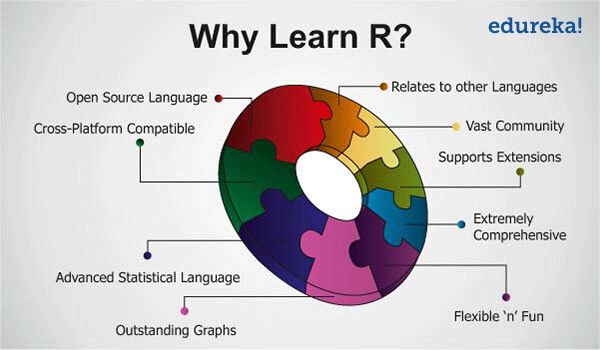
\includegraphics{./tex2pdf.956/364f0e44020784f8f6fab163de30b05c0ebf3d95.png}

\end{frame}

\begin{frame}{\href{http://blog.revolutionanalytics.com/2017/06/r-community.html}{Ein
Hauptgrund - die Community}}


\includegraphics{./tex2pdf.956/415849dd5b649c98c5239b741c3eeed83870e473.png}

\end{frame}

\begin{frame}{Möglichkeiten auf dem neuesten Stand zu sein}

\begin{itemize}
\tightlist
\item
  \href{https://rweekly.org/}{rweekly}
\end{itemize}

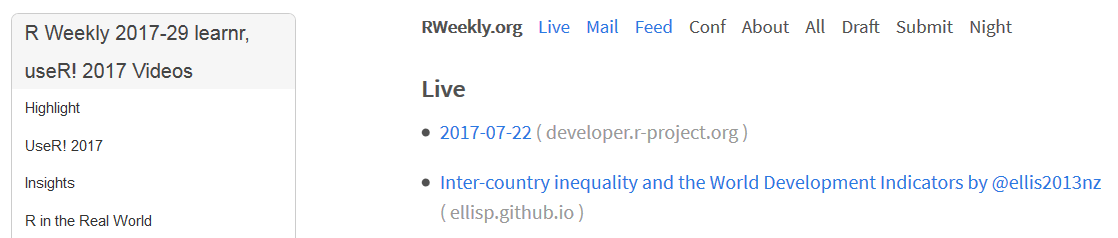
\includegraphics{./tex2pdf.956/d55db1fd3fe6749394b00af902ed3e5b81e8f49e.png}

\begin{itemize}
\tightlist
\item
  \href{https://www.r-bloggers.com/}{r-bloggers}
\end{itemize}


\includegraphics{./tex2pdf.956/76b89ea071e6ca673619294a009d8946ed81de59.png}

\end{frame}

\begin{frame}{\href{http://stats.idre.ucla.edu/r/seminars/intro/}{Modularer
Aufbau}}

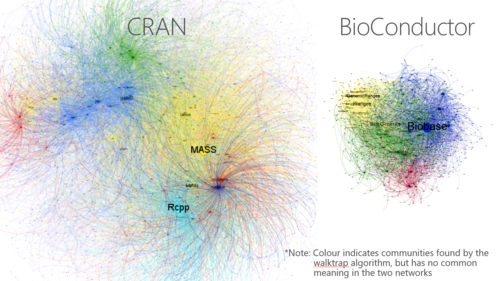
\includegraphics{./tex2pdf.956/52aa3feffd0fea76fab89e494b422bd484e53778.png}

\end{frame}

\begin{frame}{\href{https://gallery.shinyapps.io/cran-gauge/}{Viel
genutzte Pakete}}

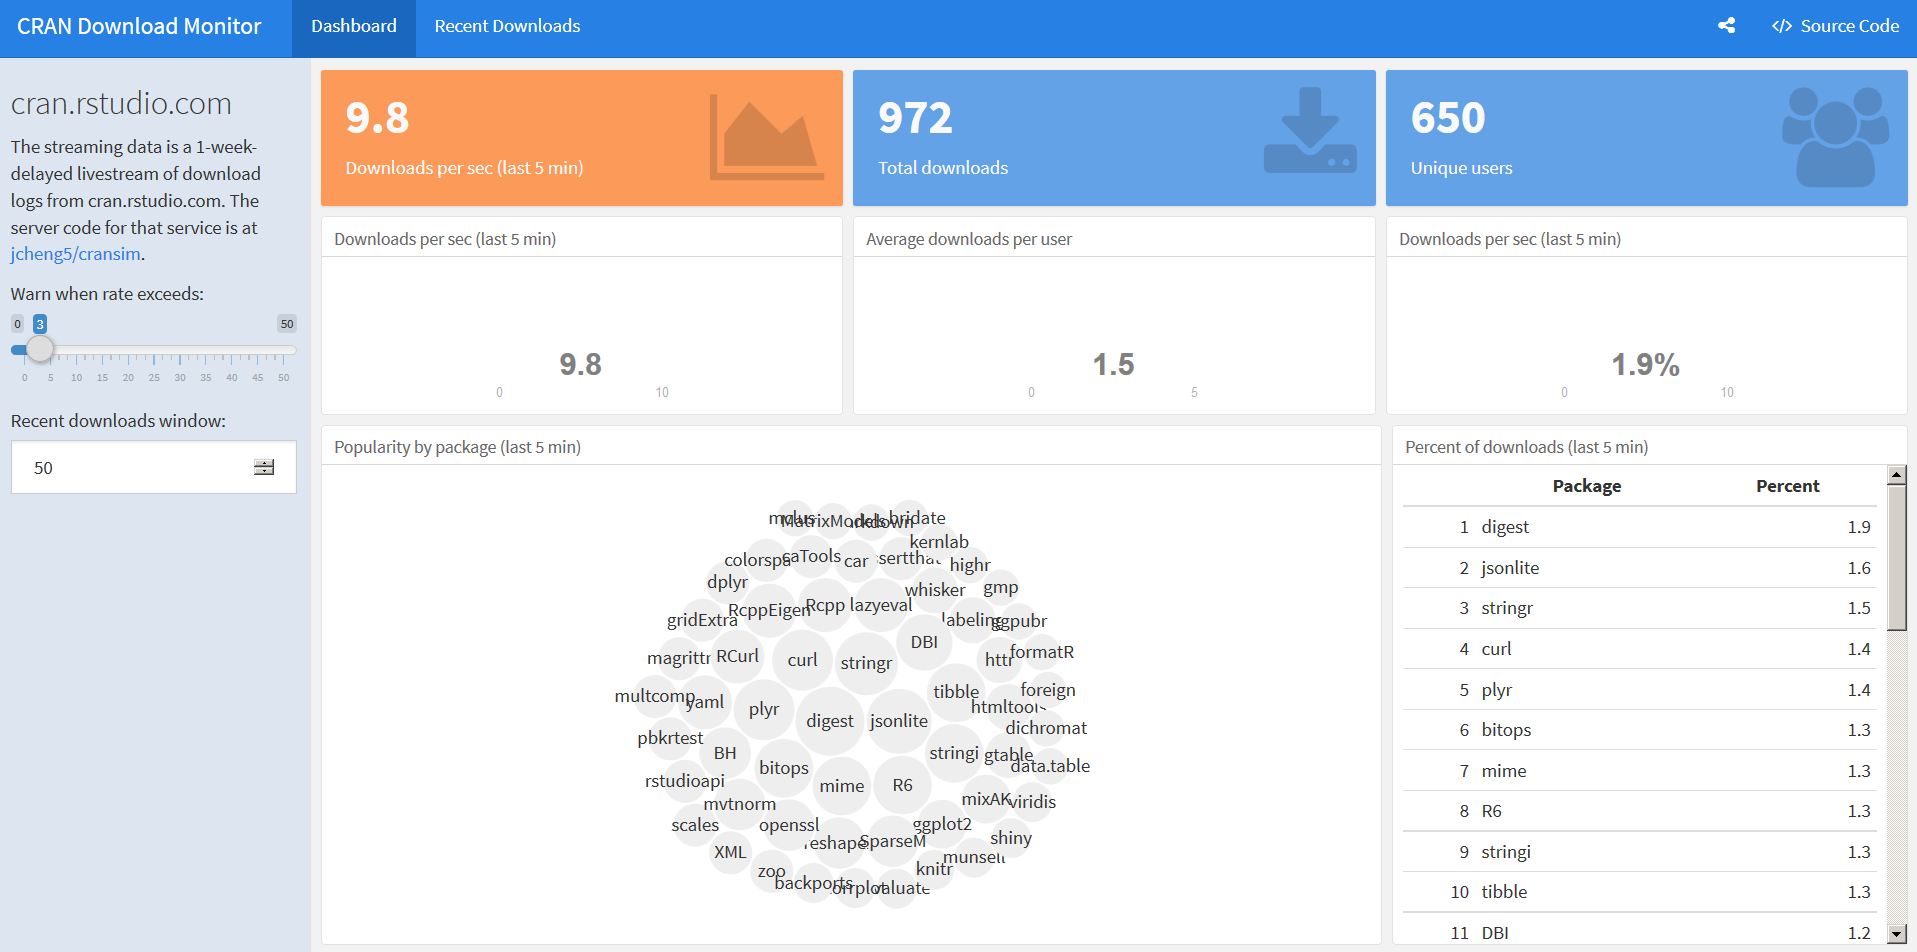
\includegraphics{./tex2pdf.956/a853199d8c52109309acb7b49e363481b04e7192.png}

\end{frame}

\begin{frame}{Organisation des Kurses}

\begin{itemize}
\tightlist
\item
  Unterlagen sind komplett auf Github hinterlegt, damit man den Kurs
  gleich mitverfolgen kann (mehr dazu gleich)
\item
  Es werden viele verschiedene kleine Beispieldatensätze verwendet um
  spezifische Dinge zu zeigen
\item
  Alle Funktionen in R sind mit diesen kleinen Beispielen hinterlegt
\item
  An geeigneten Stellen verwende ich auch größere
  (sozialwissenschaftliche) Datensätze
\end{itemize}

\end{frame}

\begin{frame}{Dem Kurs folgen}

\begin{itemize}
\tightlist
\item
  \url{http://japhilko.github.io/Rinter/}
\end{itemize}

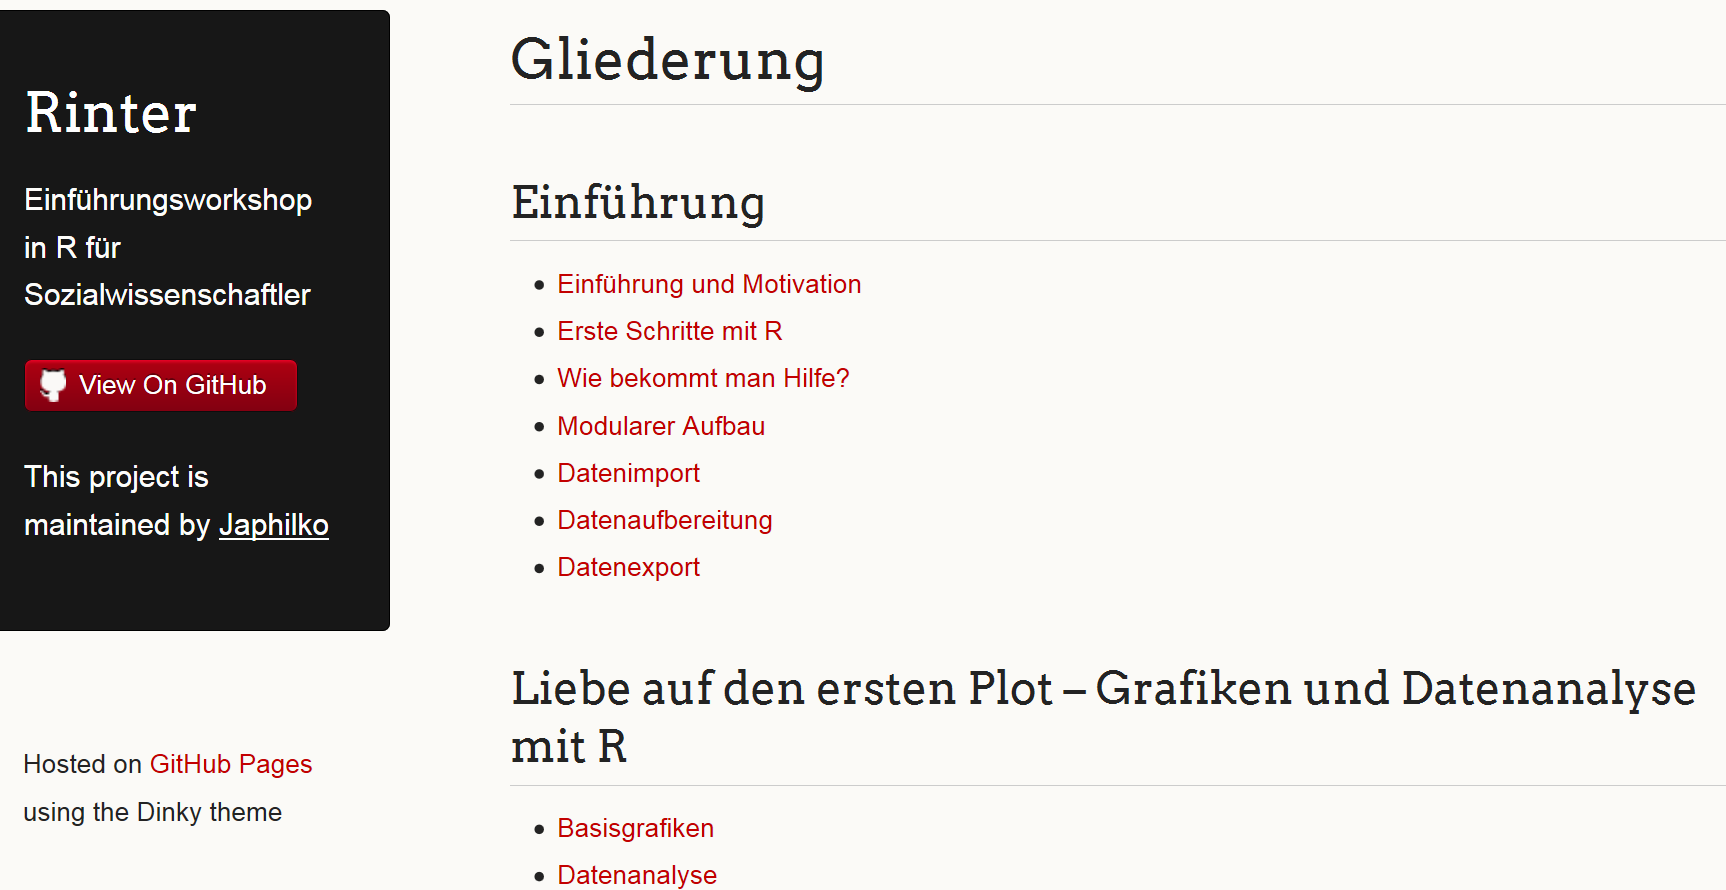
\includegraphics{./tex2pdf.956/e5396dc35519dd7e8a956d83df6bf7985683ee7e.png}

\end{frame}

\begin{frame}{Das Wiki zum Kurs}

\begin{itemize}
\tightlist
\item
  \url{https://github.com/Japhilko/Rinter/wiki}
\end{itemize}

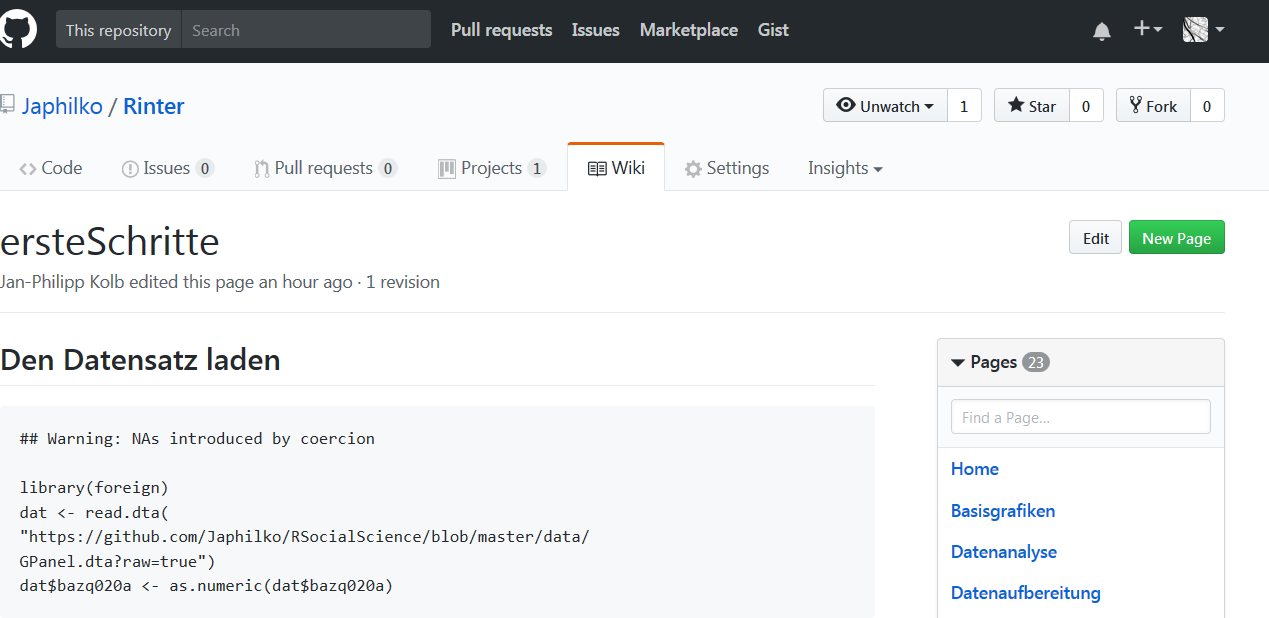
\includegraphics{./tex2pdf.956/80526e6c59606398920d3ee118ec6748029b05d2.png}

\end{frame}

\begin{frame}{Komplette Foliensätze}

Die kompletten Foliensätze kann man hier herunterladen:

\url{https://github.com/Japhilko/Rinter/blob/master/pdf_slides/R_intern.pdf}

\end{frame}

\begin{frame}{Der R-code}

\begin{itemize}
\tightlist
\item
  Den R-code kann man direkt in die R-Konsole kopieren und ausführen.
\item
  Begleitend zu den Folien wird meistens auch jeweils ein R-File
  angeboten.
\item
  Der R-code befindet sich in folgendem Ordner:
\end{itemize}

\url{https://github.com/Japhilko/RInter/tree/master/code}

\end{frame}

\begin{frame}[fragile]{Daten herunterladen}

\begin{itemize}
\item
  Vereinzelt sind auch Datensätze vorhanden.
\item
  \texttt{.csv} Dateien können direkt von R eingelesen werden (wie das
  geht, werde ich noch zeigen).
\item
  Wenn die \texttt{.csv} Dateien heruntergeladen werden sollen - den Raw
  Button verwenden.
\item
  Alle anderen Dateien (bspw. \texttt{.RData}) auch mittels Raw Button
  herunterladen.
\end{itemize}

\end{frame}

\begin{frame}{Ausdrucken}

\begin{itemize}
\item
  Zum Ausdrucken eignen sich die pdf-Dateien am besten.
\item
  Diese können mit dem Raw Button heruntergeladen werden.
\end{itemize}

\begin{block}{Raw Button bei Github}

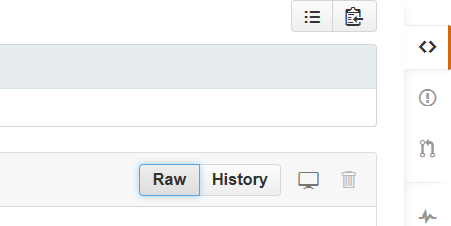
\includegraphics{./tex2pdf.956/f21c789340eb93fc24ffedb3e3f88df872b9bb2c.png}

\end{block}

\end{frame}

\begin{frame}{Basis R \ldots{}}

\begin{itemize}
\tightlist
\item
  Wenn man nur R herunterlädt und installiert, sieht das so aus:
\item
  So habe ich bis 2012 mit R gearbeitet.
\end{itemize}

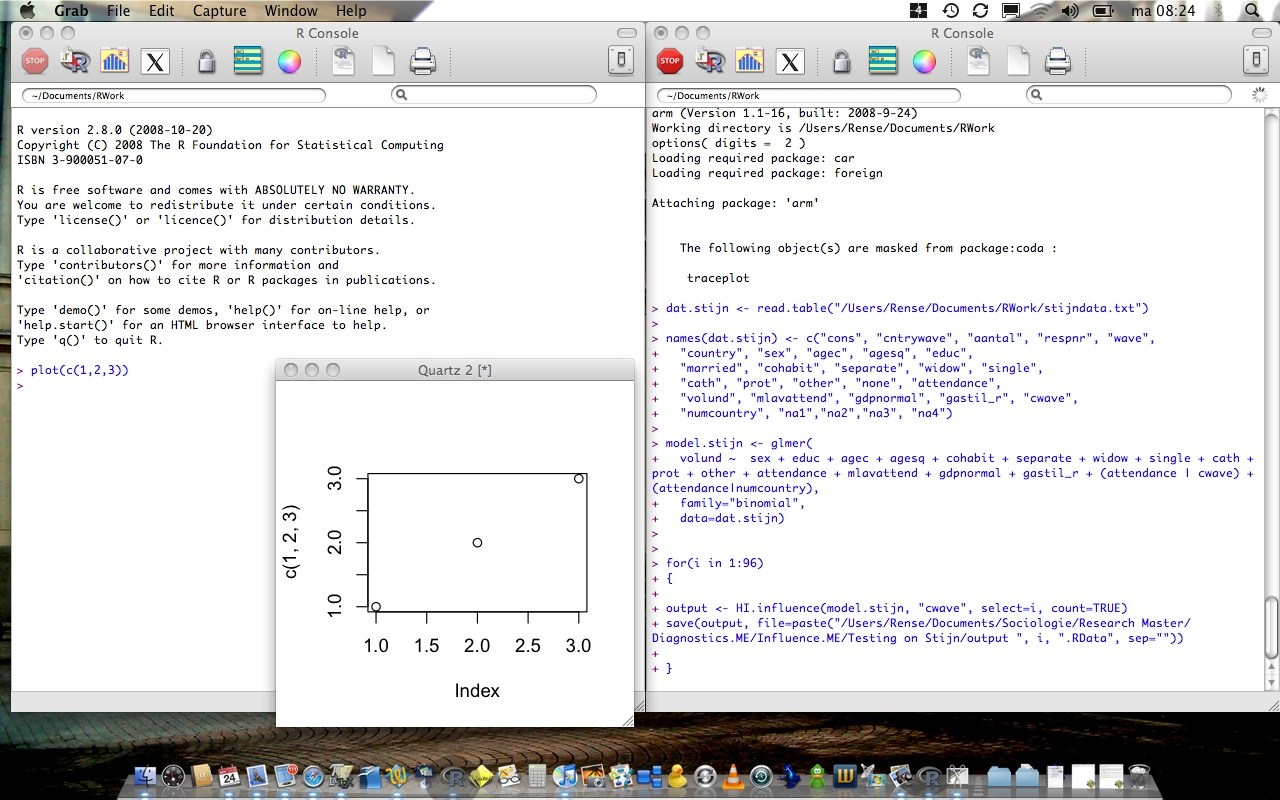
\includegraphics{./tex2pdf.956/2c652796da602b9efe1dca344441c9ada66f4fde.jpg}

\end{frame}

\begin{frame}{\ldots{} und Rstudio}

\begin{itemize}
\tightlist
\item
  Rstudio bietet Heute sehr viel Unterstützung:
\item
  und macht einige Themen dieses Workshops erst möglich
\end{itemize}

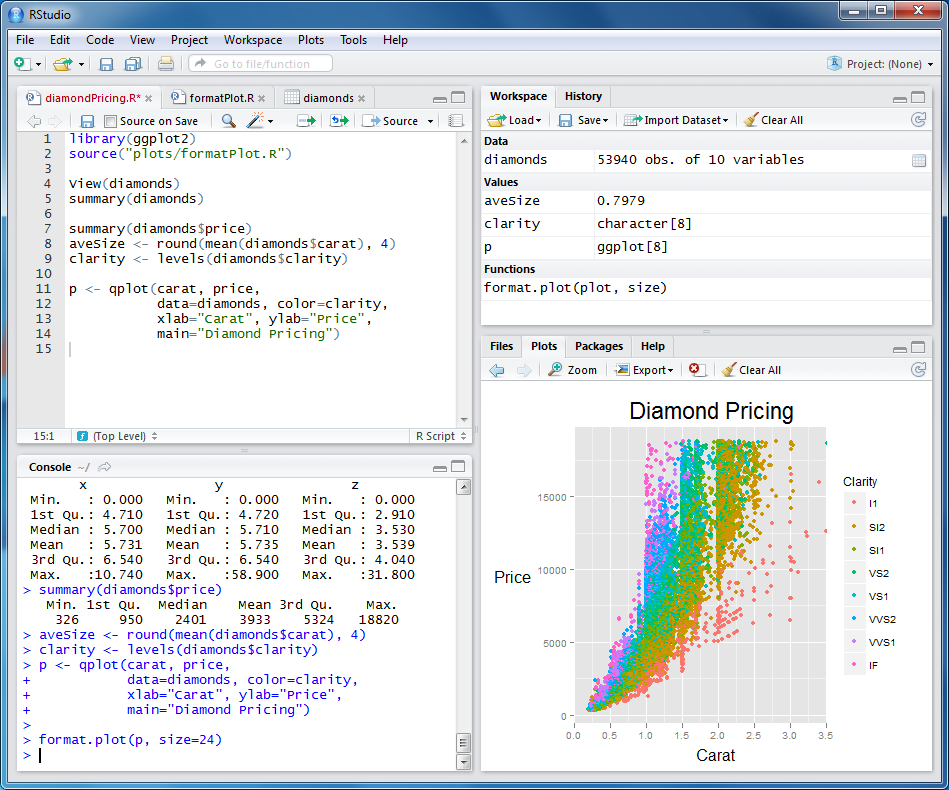
\includegraphics{./tex2pdf.956/692f3658d35df168276cf46e3e083f908a5cc105.png}

\end{frame}

\begin{frame}[fragile]{Aufgabe - Vorbereitung}

\begin{itemize}
\tightlist
\item
  Prüfen Sie, ob eine Version von R auf Rechner installiert ist.
\item
  Falls dies nicht der Fall ist, laden Sie \href{r-project.org}{R}
  runter und installieren Sie R.
\item
  Prüfen Sie, ob Rstudio installiert ist.
\item
  Falls nicht - \href{http://www.rstudio.com/}{Installieren} sie
  Rstudio.
\item
  Laden Sie die R-Skripte von meinem GitHub-Account
\item
  Erstellen Sie ein erstes Script und finden Sie das Datum mit dem
  Befehl \texttt{date()} und die R-version mit \texttt{sessionInfo()}
  heraus.
\end{itemize}

\begin{Shaded}
\begin{Highlighting}[]
\KeywordTok{date}\NormalTok{()}
\end{Highlighting}
\end{Shaded}

\begin{verbatim}
## [1] "Sun Jul 23 12:13:07 2017"
\end{verbatim}

\begin{Shaded}
\begin{Highlighting}[]
\KeywordTok{sessionInfo}\NormalTok{()}
\end{Highlighting}
\end{Shaded}

\begin{verbatim}
## R version 3.3.3 (2017-03-06)
## Platform: x86_64-w64-mingw32/x64 (64-bit)
## Running under: Windows 7 x64 (build 7601) Service Pack 1
## 
## locale:
## [1] LC_COLLATE=German_Germany.1252  LC_CTYPE=German_Germany.1252   
## [3] LC_MONETARY=German_Germany.1252 LC_NUMERIC=C                   
## [5] LC_TIME=German_Germany.1252    
## 
## attached base packages:
## [1] tools     grid      stats     graphics  grDevices utils     datasets 
## [8] methods   base     
## 
## other attached packages:
##  [1] sp_1.2-3           leaflet_1.0.1      magrittr_1.5      
##  [4] sjPlot_2.3.1       gridExtra_2.2.1    MASS_7.3-45       
##  [7] faraway_1.0.7      HSAUR_1.3-7        survey_3.31-5     
## [10] survival_2.39-5    visreg_2.3-0       DAAG_1.22         
## [13] ggmap_2.7          RColorBrewer_1.1-2 lattice_0.20-34   
## [16] beanplot_1.2       vioplot_0.2        sm_2.2-5.4        
## [19] mlmRev_1.0-6       lme4_1.1-13        Matrix_1.2-8      
## [22] knitr_1.15.20      car_2.1-4          forcats_0.2.0     
## [25] dplyr_0.5.0        purrr_0.2.2        tidyr_0.6.2       
## [28] tibble_1.3.0       ggplot2_2.2.1      tidyverse_1.1.1   
## [31] foreign_0.8-67     haven_1.0.0        readr_0.2.2       
## 
## loaded via a namespace (and not attached):
##  [1] nlme_3.1-128        bitops_1.0-6        pbkrtest_0.4-6     
##  [4] lubridate_1.5.6     httr_1.2.1          rprojroot_1.2      
##  [7] backports_1.0.5     R6_2.1.2            DT_0.2             
## [10] DBI_0.4-1           lazyeval_0.2.0      mgcv_1.8-17        
## [13] colorspace_1.2-6    nnet_7.3-12         mnormt_1.5-4       
## [16] rvest_0.3.2         quantreg_5.26       SparseM_1.7        
## [19] xml2_1.0.0          sandwich_2.3-4      effects_3.1-2      
## [22] scales_0.4.1        lmtest_0.9-34       mvtnorm_1.0-5      
## [25] psych_1.7.5         blme_1.0-4          stringr_1.2.0      
## [28] digest_0.6.12       minqa_1.2.4         rmarkdown_1.6      
## [31] stringdist_0.9.4.1  jpeg_0.1-8          htmltools_0.3.6    
## [34] maps_3.1.1          htmlwidgets_0.8     readxl_0.1.1       
## [37] shiny_1.0.3         zoo_1.7-13          jsonlite_1.4       
## [40] modeltools_0.2-21   geosphere_1.5-5     Rcpp_0.12.10       
## [43] munsell_0.4.3       abind_1.4-5         proto_1.0.0        
## [46] multcomp_1.4-6      stringi_1.1.1       yaml_2.1.14        
## [49] merTools_0.3.0      plyr_1.8.4          parallel_3.3.3     
## [52] sjmisc_2.4.0        splines_3.3.3       sjstats_0.10.0     
## [55] mapproj_1.2-4       hms_0.3             rjson_0.2.15       
## [58] codetools_0.2-15    stats4_3.3.3        reshape2_1.4.2     
## [61] evaluate_0.10       latticeExtra_0.6-28 modelr_0.0.0.9000  
## [64] httpuv_1.3.3        png_0.1-7           nloptr_1.0.4       
## [67] RgoogleMaps_1.4.1   MatrixModels_0.4-1  gtable_0.2.0       
## [70] assertthat_0.1      coin_1.1-2          mime_0.5           
## [73] xtable_1.8-2        broom_0.4.2         coda_0.19-1        
## [76] arm_1.9-3           TH.data_1.0-7
\end{verbatim}

\end{frame}

\begin{frame}{Erste Schritte mit R}

\end{frame}

\begin{frame}[fragile]{R ist eine Objekt-orientierte Sprache}

Vektoren und Zuweisungen

\begin{itemize}
\tightlist
\item
  R ist eine Objekt-orientierte Sprache
\item
  \texttt{\textless{}-} ist der Zuweisungsoperator (Shortcut: ``Alt'' +
  ``-'')
\end{itemize}

\begin{Shaded}
\begin{Highlighting}[]
\NormalTok{b <-}\StringTok{ }\KeywordTok{c}\NormalTok{(}\DecValTok{1}\NormalTok{,}\DecValTok{2}\NormalTok{) }\CommentTok{# erzeugt ein Objekt mit den Zahlen 1 und 2}
\end{Highlighting}
\end{Shaded}

\begin{itemize}
\tightlist
\item
  Eine Funktion kann auf dieses Objekt angewendet werden:
\end{itemize}

\begin{Shaded}
\begin{Highlighting}[]
\KeywordTok{mean}\NormalTok{(b) }\CommentTok{# berechnet den Mittelwert}
\end{Highlighting}
\end{Shaded}

\begin{verbatim}
## [1] 1.5
\end{verbatim}

Mit den folgenden Funktionen können wir etwas über die Eigenschaften des
Objekts lernen:

\begin{Shaded}
\begin{Highlighting}[]
\KeywordTok{length}\NormalTok{(b) }\CommentTok{# b hat die Länge 2}
\end{Highlighting}
\end{Shaded}

\begin{verbatim}
## [1] 2
\end{verbatim}

\end{frame}

\begin{frame}[fragile]{Objektstruktur - Datentypen}

\begin{Shaded}
\begin{Highlighting}[]
\KeywordTok{str}\NormalTok{(b) }\CommentTok{# b ist ein numerischer Vektor}
\end{Highlighting}
\end{Shaded}

\begin{verbatim}
##  num [1:2] 1 2
\end{verbatim}

\begin{itemize}
\tightlist
\item
  mehr zu den
  \href{http://www.statmethods.net/management/typeconversion.html}{möglichen
  Datentypen} später
\end{itemize}

\end{frame}

\begin{frame}{Funktionen im base-Paket}

\begin{longtable}[]{@{}lll@{}}
\toprule
Funktion & Bedeutung & Beispiel\tabularnewline
\midrule
\endhead
length() & Länge & length(b)\tabularnewline
max() & Maximum & max(b)\tabularnewline
min() & Minimum & min(b)\tabularnewline
sd() & Standardabweichung & sd(b)\tabularnewline
var() & Varianz & var(b)\tabularnewline
mean() & Mittelwert & mean(b)\tabularnewline
median() & Median & median(b)\tabularnewline
\bottomrule
\end{longtable}

Diese Funktionen brauchen nur ein Argument.

\end{frame}

\begin{frame}{Funktionen mit mehr Argumenten}

Andere Funktionen brauchen mehr:

\begin{longtable}[]{@{}lll@{}}
\toprule
Argument & Bedeutung & Beispiel\tabularnewline
\midrule
\endhead
quantile() & 90 \% Quantile & quantile(b,.9)\tabularnewline
sample() & Stichprobe ziehen & sample(b,1)\tabularnewline
\bottomrule
\end{longtable}

\end{frame}

\begin{frame}[fragile]{Beispiel - Funktionen mit einem Argument}

\begin{Shaded}
\begin{Highlighting}[]
\KeywordTok{max}\NormalTok{(b)}
\end{Highlighting}
\end{Shaded}

\begin{verbatim}
## [1] 2
\end{verbatim}

\begin{Shaded}
\begin{Highlighting}[]
\KeywordTok{min}\NormalTok{(b)}
\end{Highlighting}
\end{Shaded}

\begin{verbatim}
## [1] 1
\end{verbatim}

\begin{Shaded}
\begin{Highlighting}[]
\KeywordTok{sd}\NormalTok{(b)}
\end{Highlighting}
\end{Shaded}

\begin{verbatim}
## [1] 0.7071068
\end{verbatim}

\begin{Shaded}
\begin{Highlighting}[]
\KeywordTok{var}\NormalTok{(b)}
\end{Highlighting}
\end{Shaded}

\begin{verbatim}
## [1] 0.5
\end{verbatim}

\end{frame}

\begin{frame}[fragile]{Funktionen mit einem Argument}

\begin{Shaded}
\begin{Highlighting}[]
\KeywordTok{mean}\NormalTok{(b)}
\end{Highlighting}
\end{Shaded}

\begin{verbatim}
## [1] 1.5
\end{verbatim}

\begin{Shaded}
\begin{Highlighting}[]
\KeywordTok{median}\NormalTok{(b)}
\end{Highlighting}
\end{Shaded}

\begin{verbatim}
## [1] 1.5
\end{verbatim}

\end{frame}

\begin{frame}[fragile]{Funktionen mit mehr Argumenten}

\begin{Shaded}
\begin{Highlighting}[]
\KeywordTok{quantile}\NormalTok{(b,.}\DecValTok{9}\NormalTok{)}
\end{Highlighting}
\end{Shaded}

\begin{verbatim}
## 90% 
## 1.9
\end{verbatim}

\begin{Shaded}
\begin{Highlighting}[]
\KeywordTok{sample}\NormalTok{(b,}\DecValTok{1}\NormalTok{) }
\end{Highlighting}
\end{Shaded}

\begin{verbatim}
## [1] 2
\end{verbatim}

\end{frame}

\begin{frame}{\href{http://cran.r-project.org/doc/manuals/R-intro.html}{Übersicht
Befehle}}

\url{http://cran.r-project.org/doc/manuals/R-intro.html}

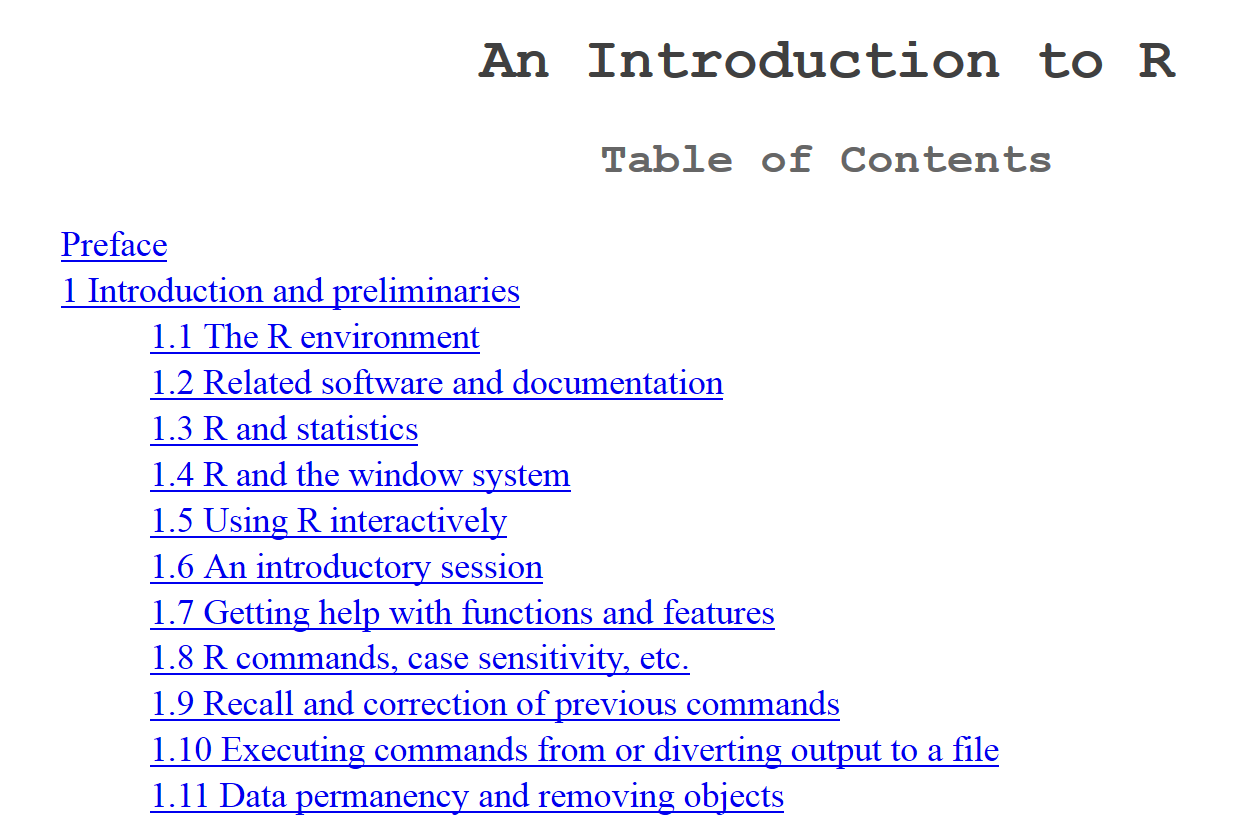
\includegraphics{./tex2pdf.956/5d240a600e94270437008ff177d88aceaa547418.png}

\end{frame}

\begin{frame}{Aufgabe - Zuweisungen und Funktionen}

Erzeugt einen Vektor b mit den Zahlen von 1 bis 5 und berechnet\ldots{}

\begin{enumerate}
\def\labelenumi{\arabic{enumi}.}
\item
  den Mittelwert
\item
  die Varianz
\item
  die Standardabweichung
\item
  die quadratische Wurzel aus dem Mittelwert
\end{enumerate}

\end{frame}

\begin{frame}[fragile]{Verschiedene Datentypen}

\begin{longtable}[]{@{}lll@{}}
\toprule
Datentyp & Beschreibung & Beispiel\tabularnewline
\midrule
\endhead
numeric & ganze und reele Zahlen & \texttt{5,\ 3.462}\tabularnewline
logical & logische Werte & \texttt{FALSE,\ TRUE}\tabularnewline
character & Buchstaben und Zeichenfolgen &
\texttt{"Hallo"}\tabularnewline
\bottomrule
\end{longtable}

Quelle:
\href{https://www.uni-trier.de/fileadmin/fb4/prof/VWL/FIN/Oekonometrie/PC-UEbung/Einfuehrung_in_R.pdf}{R.
Münnich und M. Knobelspieß} (2007): Einführung in das statistische
Programmpaket R

\end{frame}

\begin{frame}[fragile]{Verschiedene Datentypen}

\begin{Shaded}
\begin{Highlighting}[]
\NormalTok{b <-}\StringTok{ }\KeywordTok{c}\NormalTok{(}\DecValTok{1}\NormalTok{,}\DecValTok{2}\NormalTok{) }\CommentTok{# numeric}
\NormalTok{log <-}\StringTok{ }\KeywordTok{c}\NormalTok{(T,F) }\CommentTok{# logical}
\NormalTok{char <-}\KeywordTok{c}\NormalTok{(}\StringTok{"A"}\NormalTok{,}\StringTok{"b"}\NormalTok{) }\CommentTok{# character}
\NormalTok{fac <-}\StringTok{ }\KeywordTok{as.factor}\NormalTok{(}\KeywordTok{c}\NormalTok{(}\DecValTok{1}\NormalTok{,}\DecValTok{2}\NormalTok{)) }\CommentTok{# factor}
\end{Highlighting}
\end{Shaded}

Mit \texttt{str()} bekommt man den Objekttyp.

\begin{Shaded}
\begin{Highlighting}[]
\KeywordTok{str}\NormalTok{(fac)}
\end{Highlighting}
\end{Shaded}

\begin{verbatim}
##  Factor w/ 2 levels "1","2": 1 2
\end{verbatim}

\end{frame}

\begin{frame}[fragile]{Indizieren eines Vektors:}

\begin{Shaded}
\begin{Highlighting}[]
\NormalTok{A1 <-}\StringTok{ }\KeywordTok{c}\NormalTok{(}\DecValTok{1}\NormalTok{,}\DecValTok{2}\NormalTok{,}\DecValTok{3}\NormalTok{,}\DecValTok{4}\NormalTok{)}
\NormalTok{A1}
\end{Highlighting}
\end{Shaded}

\begin{verbatim}
## [1] 1 2 3 4
\end{verbatim}

\begin{Shaded}
\begin{Highlighting}[]
\NormalTok{A1[}\DecValTok{1}\NormalTok{]}
\end{Highlighting}
\end{Shaded}

\begin{verbatim}
## [1] 1
\end{verbatim}

\begin{Shaded}
\begin{Highlighting}[]
\NormalTok{A1[}\DecValTok{4}\NormalTok{]}
\end{Highlighting}
\end{Shaded}

\begin{verbatim}
## [1] 4
\end{verbatim}

\begin{Shaded}
\begin{Highlighting}[]
\NormalTok{A1[}\DecValTok{1}\NormalTok{:}\DecValTok{3}\NormalTok{]}
\end{Highlighting}
\end{Shaded}

\begin{verbatim}
## [1] 1 2 3
\end{verbatim}

\begin{Shaded}
\begin{Highlighting}[]
\NormalTok{A1[-}\DecValTok{4}\NormalTok{]}
\end{Highlighting}
\end{Shaded}

\begin{verbatim}
## [1] 1 2 3
\end{verbatim}

\end{frame}

\begin{frame}[fragile]{Logische Operatoren}

\begin{Shaded}
\begin{Highlighting}[]
\CommentTok{# Ist 1 größer als 2?}
\DecValTok{1}\NormalTok{>}\DecValTok{2}
\end{Highlighting}
\end{Shaded}

\begin{verbatim}
## [1] FALSE
\end{verbatim}

\begin{Shaded}
\begin{Highlighting}[]
\DecValTok{1}\NormalTok{<}\DecValTok{2}
\end{Highlighting}
\end{Shaded}

\begin{verbatim}
## [1] TRUE
\end{verbatim}

\begin{Shaded}
\begin{Highlighting}[]
\DecValTok{1}\NormalTok{==}\DecValTok{2}
\end{Highlighting}
\end{Shaded}

\begin{verbatim}
## [1] FALSE
\end{verbatim}

\end{frame}

\begin{frame}[fragile]{Sequenzen}

\begin{Shaded}
\begin{Highlighting}[]
\CommentTok{# Sequenz von 1 bis 10}
\DecValTok{1}\NormalTok{:}\DecValTok{10}
\end{Highlighting}
\end{Shaded}

\begin{verbatim}
##  [1]  1  2  3  4  5  6  7  8  9 10
\end{verbatim}

\begin{Shaded}
\begin{Highlighting}[]
\CommentTok{# das gleiche Ergebnis}
\KeywordTok{seq}\NormalTok{(}\DecValTok{1}\NormalTok{,}\DecValTok{10}\NormalTok{)}
\end{Highlighting}
\end{Shaded}

\begin{verbatim}
##  [1]  1  2  3  4  5  6  7  8  9 10
\end{verbatim}

\end{frame}

\begin{frame}[fragile]{Weitere Sequenzen}

\begin{Shaded}
\begin{Highlighting}[]
\KeywordTok{seq}\NormalTok{(-}\DecValTok{2}\NormalTok{,}\DecValTok{8}\NormalTok{,}\DataTypeTok{by=}\FloatTok{1.5}\NormalTok{)}
\end{Highlighting}
\end{Shaded}

\begin{verbatim}
## [1] -2.0 -0.5  1.0  2.5  4.0  5.5  7.0
\end{verbatim}

\begin{Shaded}
\begin{Highlighting}[]
\NormalTok{a <-}\KeywordTok{seq}\NormalTok{(}\DecValTok{3}\NormalTok{,}\DecValTok{12}\NormalTok{,}\DataTypeTok{length=}\DecValTok{12}\NormalTok{)}
\NormalTok{a}
\end{Highlighting}
\end{Shaded}

\begin{verbatim}
##  [1]  3.000000  3.818182  4.636364  5.454545  6.272727  7.090909  7.909091
##  [8]  8.727273  9.545455 10.363636 11.181818 12.000000
\end{verbatim}

\begin{Shaded}
\begin{Highlighting}[]
\NormalTok{b <-}\StringTok{ }\KeywordTok{seq}\NormalTok{(}\DataTypeTok{to=}\DecValTok{5}\NormalTok{,}\DataTypeTok{length=}\DecValTok{12}\NormalTok{,}\DataTypeTok{by=}\FloatTok{0.2}\NormalTok{)}
\NormalTok{b}
\end{Highlighting}
\end{Shaded}

\begin{verbatim}
##  [1] 2.8 3.0 3.2 3.4 3.6 3.8 4.0 4.2 4.4 4.6 4.8 5.0
\end{verbatim}

\end{frame}

\begin{frame}[fragile]{Reihenfolge von Argumenten}

\begin{Shaded}
\begin{Highlighting}[]
\DecValTok{1}\NormalTok{:}\DecValTok{10}
\end{Highlighting}
\end{Shaded}

\begin{verbatim}
##  [1]  1  2  3  4  5  6  7  8  9 10
\end{verbatim}

\begin{Shaded}
\begin{Highlighting}[]
\KeywordTok{seq}\NormalTok{(}\DecValTok{1}\NormalTok{,}\DecValTok{10}\NormalTok{,}\DecValTok{1}\NormalTok{)}
\end{Highlighting}
\end{Shaded}

\begin{verbatim}
##  [1]  1  2  3  4  5  6  7  8  9 10
\end{verbatim}

\begin{Shaded}
\begin{Highlighting}[]
\KeywordTok{seq}\NormalTok{(}\DataTypeTok{length=}\DecValTok{10}\NormalTok{,}\DataTypeTok{from=}\DecValTok{1}\NormalTok{,}\DataTypeTok{by=}\DecValTok{1}\NormalTok{)}
\end{Highlighting}
\end{Shaded}

\begin{verbatim}
##  [1]  1  2  3  4  5  6  7  8  9 10
\end{verbatim}

\end{frame}

\begin{frame}[fragile]{Wiederholungen}

\begin{Shaded}
\begin{Highlighting}[]
\CommentTok{# wiederhole 1 10 mal}
\KeywordTok{rep}\NormalTok{(}\DecValTok{1}\NormalTok{,}\DecValTok{10}\NormalTok{)}
\end{Highlighting}
\end{Shaded}

\begin{verbatim}
##  [1] 1 1 1 1 1 1 1 1 1 1
\end{verbatim}

\begin{Shaded}
\begin{Highlighting}[]
\KeywordTok{rep}\NormalTok{(}\StringTok{"A"}\NormalTok{,}\DecValTok{10}\NormalTok{)}
\end{Highlighting}
\end{Shaded}

\begin{verbatim}
##  [1] "A" "A" "A" "A" "A" "A" "A" "A" "A" "A"
\end{verbatim}

\end{frame}

\begin{frame}[fragile]{Die Funktion paste}

\begin{Shaded}
\begin{Highlighting}[]
\NormalTok{?paste}
\end{Highlighting}
\end{Shaded}

\begin{Shaded}
\begin{Highlighting}[]
\KeywordTok{paste}\NormalTok{(}\DecValTok{1}\NormalTok{:}\DecValTok{4}\NormalTok{)}
\end{Highlighting}
\end{Shaded}

\begin{verbatim}
## [1] "1" "2" "3" "4"
\end{verbatim}

\begin{Shaded}
\begin{Highlighting}[]
\KeywordTok{paste}\NormalTok{(}\StringTok{"A"}\NormalTok{, }\DecValTok{1}\NormalTok{:}\DecValTok{6}\NormalTok{, }\DataTypeTok{sep =} \StringTok{""}\NormalTok{)}
\end{Highlighting}
\end{Shaded}

\begin{verbatim}
## [1] "A1" "A2" "A3" "A4" "A5" "A6"
\end{verbatim}

\begin{itemize}
\tightlist
\item
  Ein weiteres Beispiel:
\end{itemize}

\begin{Shaded}
\begin{Highlighting}[]
\KeywordTok{paste0}\NormalTok{(}\StringTok{"A"}\NormalTok{, }\DecValTok{1}\NormalTok{:}\DecValTok{6}\NormalTok{)}
\end{Highlighting}
\end{Shaded}

\begin{verbatim}
## [1] "A1" "A2" "A3" "A4" "A5" "A6"
\end{verbatim}

\end{frame}

\begin{frame}{Wie bekommt man Hilfe?}

\end{frame}

\begin{frame}[fragile]{Wie bekommt man Hilfe?}

\begin{itemize}
\tightlist
\item
  \href{http://itfeature.com/tag/how-to-get-help-in-r}{Um generell Hilfe
  zu bekommen:}
\end{itemize}

\begin{Shaded}
\begin{Highlighting}[]
\KeywordTok{help.start}\NormalTok{()}
\end{Highlighting}
\end{Shaded}

\begin{itemize}
\tightlist
\item
  \href{https://www.r-project.org/help.html}{Online Dokumentation für
  die meisten Funktionen:}
\end{itemize}

\begin{Shaded}
\begin{Highlighting}[]
\KeywordTok{help}\NormalTok{(name)}
\end{Highlighting}
\end{Shaded}

\begin{itemize}
\tightlist
\item
  Nutze ? um Hilfe zu bekommen.
\end{itemize}

\begin{Shaded}
\begin{Highlighting}[]
\NormalTok{?mean}
\end{Highlighting}
\end{Shaded}

\begin{itemize}
\tightlist
\item
  example(lm) gibt ein Beispiel für die lineare Regression
\end{itemize}

\begin{Shaded}
\begin{Highlighting}[]
\KeywordTok{example}\NormalTok{(lm)}
\end{Highlighting}
\end{Shaded}

\end{frame}

\begin{frame}[fragile]{Vignetten}

\begin{itemize}
\tightlist
\item
  Dokumente zur Veranschaulichung und Erläuterung von Funktionen im
  Paket
\end{itemize}

\begin{Shaded}
\begin{Highlighting}[]
\KeywordTok{browseVignettes}\NormalTok{()}
\end{Highlighting}
\end{Shaded}

\end{frame}

\begin{frame}[fragile]{Demos}

\begin{itemize}
\tightlist
\item
  zu manchem Paketen gibt es Demonstrationen, wie der Code zu verwenden
  ist
\end{itemize}

\begin{Shaded}
\begin{Highlighting}[]
\KeywordTok{demo}\NormalTok{()}
\KeywordTok{demo}\NormalTok{(nlm)}
\end{Highlighting}
\end{Shaded}

\end{frame}

\begin{frame}[fragile]{Die Funktion \texttt{apropos}}

\begin{itemize}
\tightlist
\item
  sucht alles, was mit dem eingegebenen String in Verbindung steht
\end{itemize}

\begin{Shaded}
\begin{Highlighting}[]
\KeywordTok{apropos}\NormalTok{(}\StringTok{"lm"}\NormalTok{)}
\end{Highlighting}
\end{Shaded}

\begin{verbatim}
##  [1] ".__C__anova.glm"      ".__C__anova.glm.null" ".__C__diagonalMatrix"
##  [4] ".__C__generalMatrix"  ".__C__glm"            ".__C__glm.null"      
##  [7] ".__C__glmerMod"       ".__C__lm"             ".__C__lMatrix"       
## [10] ".__C__lmerMod"        ".__C__lmList4"        ".__C__mlm"           
## [13] ".__C__nlmerMod"       ".__C__optionalMethod" ".__T__colMeans:base" 
## [16] ".__T__getL:lme4"      ".colMeans"            ".lm.fit"             
## [19] "colMeans"             "colMeans"             "confint.lm"          
## [22] "contr.helmert"        "contr.Helmert"        "cv.lm"               
## [25] "CVlm"                 "dummy.coef.lm"        "getAllMethods"       
## [28] "glm"                  "glm.control"          "glm.fit"             
## [31] "glmer"                "glmer.nb"             "glmerControl"        
## [34] "glmerLaplaceHandle"   "glmFamily"            "glmResp"             
## [37] "isGLMM"               "isLMM"                "isNLMM"              
## [40] "KalmanForecast"       "KalmanLike"           "KalmanRun"           
## [43] "KalmanSmooth"         "kappa.lm"             "lm"                  
## [46] "lm.fit"               "lm.influence"         "lm.wfit"             
## [49] "lmap"                 "lmap_at"              "lmap_if"             
## [52] "lmdiags"              "lmer"                 "lmerControl"         
## [55] "lmerResp"             "lmList"               "lmResp"              
## [58] "marginalModelPlot"    "marginalModelPlots"   "mkGlmerDevfun"       
## [61] "mkLmerDevfun"         "model.matrix.lm"      "nlm"                 
## [64] "nlmer"                "nlmerControl"         "nlminb"              
## [67] "optimizeGlmer"        "optimizeLmer"         "panel.lmline"        
## [70] "predict.glm"          "predict.lm"           "prepanel.lmline"     
## [73] "residuals.glm"        "residuals.lm"         "summary.glm"         
## [76] "summary.lm"           "svyglm"               "updateGlmerDevfun"
\end{verbatim}

\begin{itemize}
\tightlist
\item
  man kann das auch in Verbindung mit regulären Ausdrücken verwenden
\end{itemize}

\begin{Shaded}
\begin{Highlighting}[]
\NormalTok{?}\StringTok{"regular expression"}
\end{Highlighting}
\end{Shaded}

\begin{Shaded}
\begin{Highlighting}[]
\KeywordTok{help.search}\NormalTok{(}\StringTok{"^glm"}\NormalTok{)}
\end{Highlighting}
\end{Shaded}

\end{frame}

\begin{frame}[fragile]{\href{http://search.r-project.org/cgi-bin/namazu.cgi?query=glm\&max=20\&result=normal\&sort=score\&idxname=functions\&idxname=vignettes\&idxname=views}{Suchmaschine
für die R-Seite}}

\begin{Shaded}
\begin{Highlighting}[]
\KeywordTok{RSiteSearch}\NormalTok{(}\StringTok{"glm"}\NormalTok{)}
\end{Highlighting}
\end{Shaded}

\end{frame}

\begin{frame}[fragile]{Nutzung Suchmaschinen}

\begin{itemize}
\tightlist
\item
  Ich nutze meistens google
\item
  Tippe:
\end{itemize}

\begin{verbatim}
R-project + Was ich schon immer wissen wollte
\end{verbatim}

\begin{itemize}
\tightlist
\item
  Das funktioniert natürlich mit jeder Suchmaschine!
\end{itemize}

\end{frame}

\begin{frame}{\href{http://stackoverflow.com/}{Stackoverflow}}

\begin{itemize}
\tightlist
\item
  Für Fragen zum Programmieren
\item
  \href{https://stackoverflow.com/tags/r/info}{Ist nicht auf R
  fokussiert, es gibt aber viele Diskussionen zu R}
\item
  Sehr detailierte Diskussionen
\end{itemize}

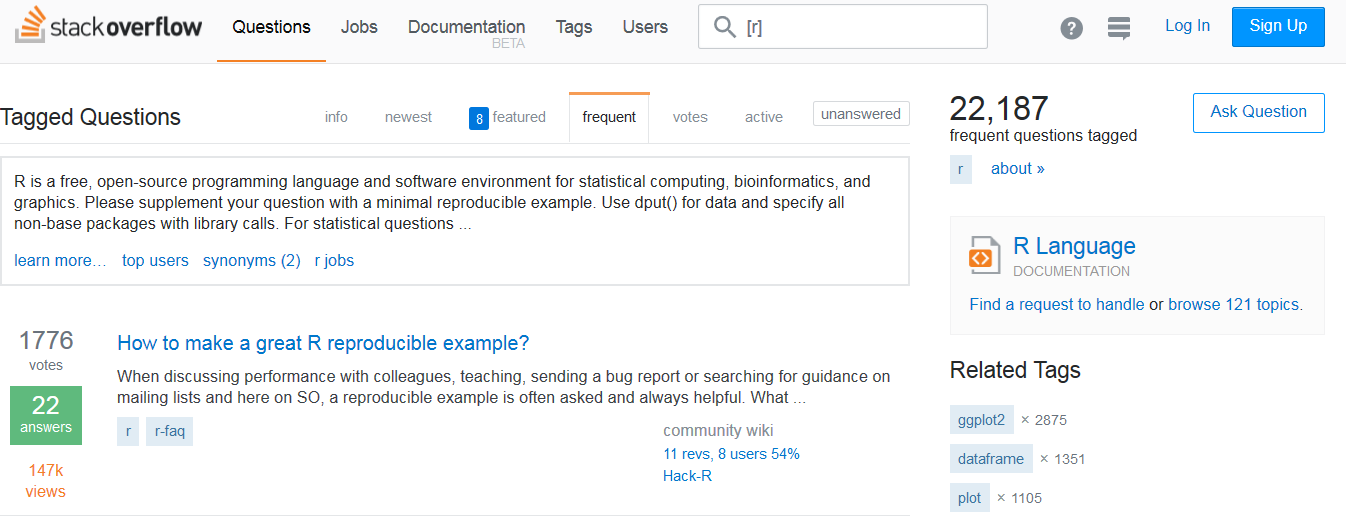
\includegraphics{./tex2pdf.956/b355b991b8b67437045666b49510802f4d9ef989.png}

\end{frame}

\begin{frame}{\href{http://www.statmethods.net/interface/help.html}{Quick
R}}

\begin{block}{Quick R}

\begin{itemize}
\tightlist
\item
  Eine Seite mit Beispielen und Hilfe zu einem Thema
\item
  Beispiel: \href{http://www.statmethods.net/interface/help.html}{Quick
  R - Getting Help}
\end{itemize}

\end{block}

\begin{block}{Weitere Links}

\begin{itemize}
\item
  \href{https://www.r-project.org/help.html}{Übersicht - Hilfe bekommen
  in R}
\item
  \href{http://rprogramming.net/}{Eine Liste mit HowTo`s}
\item
  \href{https://www.personality-project.org/r/r.commands.html}{Eine
  Liste der wichtigsten R-Befehle}
\end{itemize}

\end{block}

\end{frame}

\begin{frame}{Ein Schummelzettel - Cheatsheet}

\url{https://www.rstudio.com/resources/cheatsheets/}

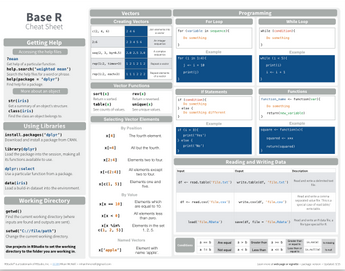
\includegraphics{./tex2pdf.956/7d1907fc7cfa03bf0f3e2ee3123fcb07ca60f41c.png}

\end{frame}

\begin{frame}{Modularer Aufbau}

\end{frame}

\begin{frame}{\href{https://stats.idre.ucla.edu/r/seminars/intro/}{Wo
sind die Funktionen enthalten}}

\begin{itemize}
\tightlist
\item
  Viele Funktionen sind im Basis-R enthalten
\item
  Viele spezifische Funktionen sind in zusätzlichen Bibliotheken
  integriert
\item
  R kann modular erweitert werden durch sog. packages bzw. libraries
\item
  Auf CRAN werden die wichtigsten packages gehostet (im Moment 11020)
\item
  Mehr Pakete (v.a. Biostatistik, Medizin) finden sich z.B. bei
  \href{www.bioconductor.org}{bioconductor}
\end{itemize}

\end{frame}

\begin{frame}{Übersicht R-Pakete}

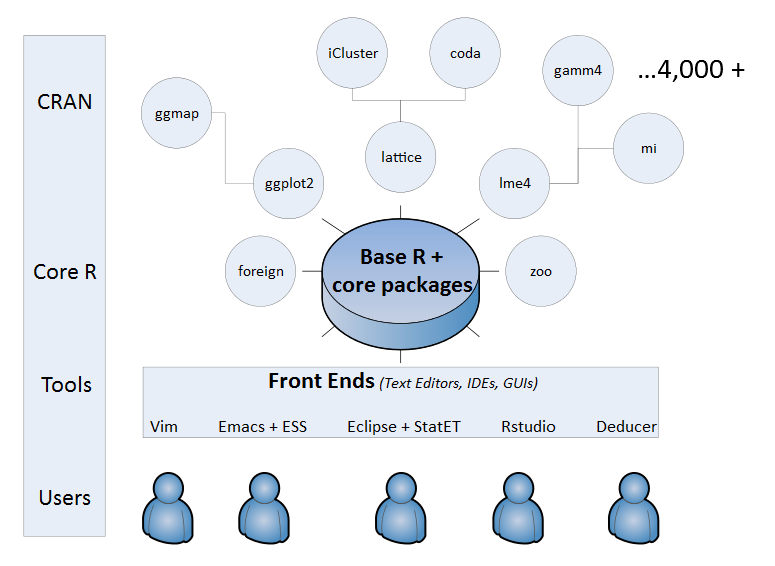
\includegraphics{./tex2pdf.956/6246b503fa80f41683217b14cc9372e5ef61a781.png}

\end{frame}

\begin{frame}[fragile]{Installation}

\begin{Shaded}
\begin{Highlighting}[]
\KeywordTok{install.packages}\NormalTok{(}\StringTok{"lme4"}\NormalTok{)}

\KeywordTok{library}\NormalTok{(lme4)}
\end{Highlighting}
\end{Shaded}

\end{frame}

\begin{frame}{Installation von Paketen mit RStudio}

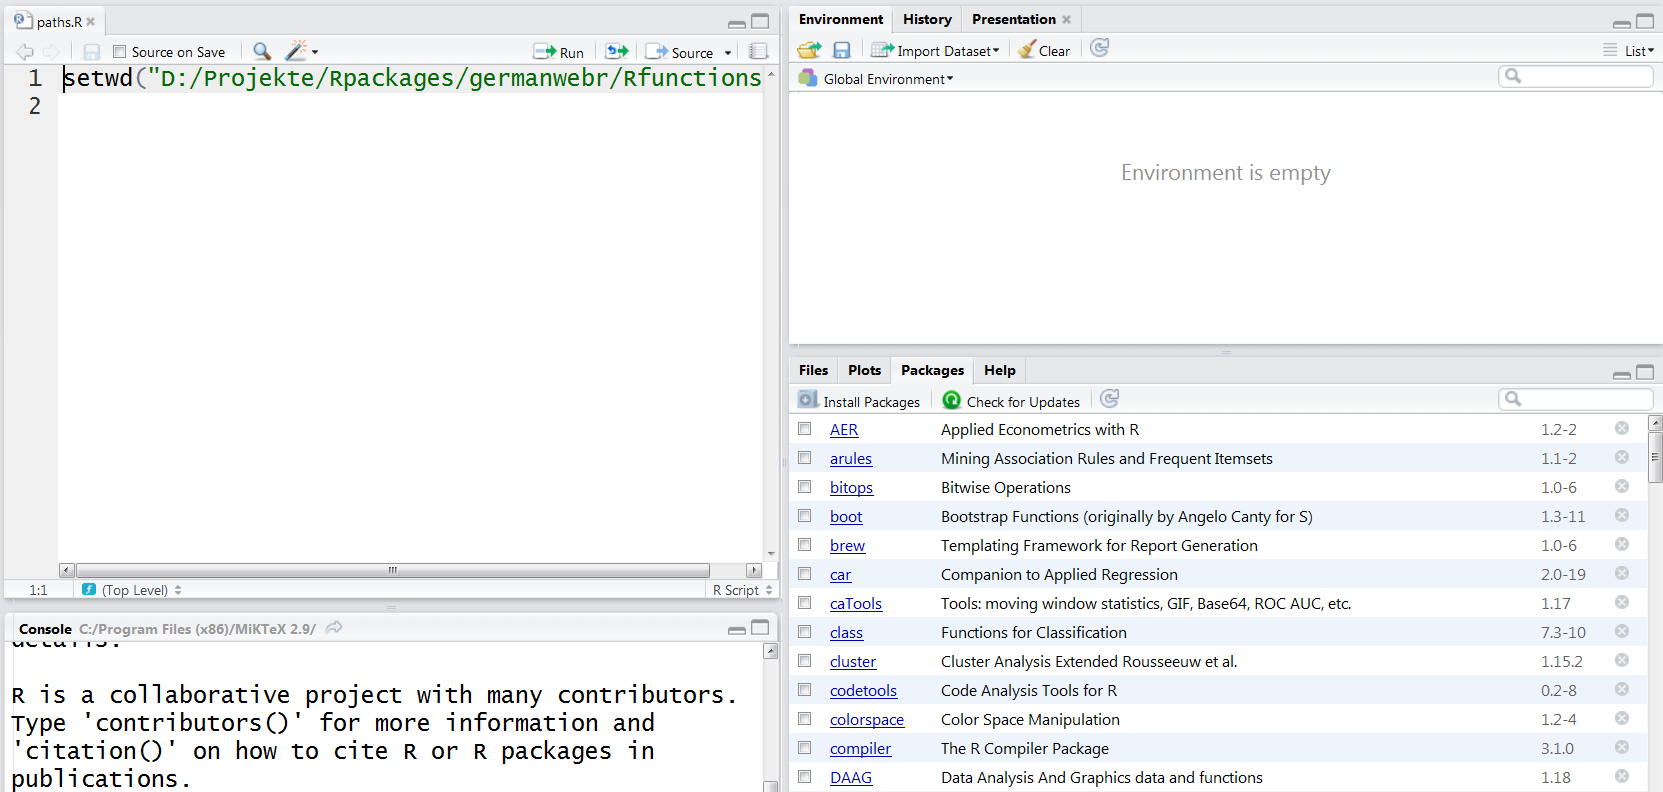
\includegraphics{./tex2pdf.956/c6c143900ad8bf587abcf5f17c830e0628827a25.png}

\end{frame}

\begin{frame}{Vorhandene Pakete und Installation}

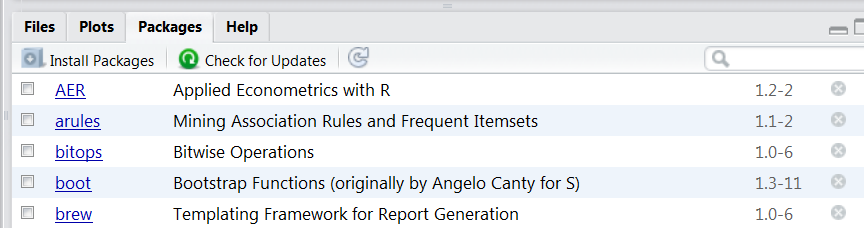
\includegraphics{./tex2pdf.956/0af3f1dcb1917a9b105b8ccb6be1cf1a459287cd.png}

\end{frame}

\begin{frame}[fragile]{Übersicht viele nützliche Pakete:}

\begin{itemize}
\tightlist
\item
  Luhmann -
  \href{http://www.beltz.de/fileadmin/beltz/downloads/OnlinematerialienPVU/28090_Luhmann/Verwendete\%20Pakete.pdf}{Tabelle
  mit vielen nützlichen Paketen}
\end{itemize}

\begin{block}{Weitere interessante Pakete:}

\begin{itemize}
\item
  Paket für den Import/Export -
  \href{http://cran.r-project.org/web/packages/foreign/foreign.pdf}{foreign}
\item
  \href{http://iase-web.org/documents/papers/icots8/ICOTS8_4J1_TILLE.pdf}{Pakete
  für Survey Sampling}
\item
  \texttt{xtable} Paket für die Integration von Latex und R
  (\href{http://cran.r-project.org/web/packages/xtable/vignettes/xtableGallery.pdf}{xtable
  Galerie})
\item
  \href{http://cran.r-project.org/web/packages/dummies/dummies.pdf}{Paket
  zur Erzeugung von Dummies}
\item
  \href{http://cran.r-project.org/web/packages/mvtnorm/index.html}{Multivariate
  Normalverteilung}
\item
  \href{http://www.r-bloggers.com/tag/maptools/}{Paket für Karten}
\end{itemize}

\end{block}

\end{frame}

\begin{frame}[fragile]{Pakete installieren}

\begin{block}{Pakete von CRAN Server installieren}

\begin{Shaded}
\begin{Highlighting}[]
\KeywordTok{install.packages}\NormalTok{(}\StringTok{"lme4"}\NormalTok{)}
\end{Highlighting}
\end{Shaded}

\end{block}

\begin{block}{Pakete von Bioconductor Server installieren}

\begin{Shaded}
\begin{Highlighting}[]
\KeywordTok{source}\NormalTok{(}\StringTok{"https://bioconductor.org/biocLite.R"}\NormalTok{)}
\KeywordTok{biocLite}\NormalTok{(}\KeywordTok{c}\NormalTok{(}\StringTok{"GenomicFeatures"}\NormalTok{, }\StringTok{"AnnotationDbi"}\NormalTok{))}
\end{Highlighting}
\end{Shaded}

\end{block}

\begin{block}{Pakete von Github installieren}

\begin{Shaded}
\begin{Highlighting}[]
\KeywordTok{install.packages}\NormalTok{(}\StringTok{"devtools"}\NormalTok{)}
\KeywordTok{library}\NormalTok{(devtools)}

\KeywordTok{install_github}\NormalTok{(}\StringTok{"hadley/ggplot2"}\NormalTok{)}
\end{Highlighting}
\end{Shaded}

\end{block}

\end{frame}

\begin{frame}{Wie bekomme ich einen Überblick}

\begin{itemize}
\item
  \href{https://mran.microsoft.com/packages/}{Pakete entdecken, die
  neulich auf CRAN hochgeladen wurden}
\item
  \href{https://gallery.shinyapps.io/cran-gauge/}{Pakete nachschauen,
  die in letzter Zeit von CRAN heruntergeladen wurden}
\item
  \href{https://support.rstudio.com/hc/en-us/articles/201057987-Quick-list-of-useful-R-packages}{Eine
  Quick-list nützlicher Pakete} auf der Support Seite von Rstudio
\item
  Computerworld hat die
  \href{http://www.computerworld.com/article/2921176/business-intelligence/great-r-packages-for-data-import-wrangling-visualization.html}{besten
  Pakete für Datenbearbeitung und Analyse} aufgelistet
\item
  Auf R-Bloggers gibt es eine Liste mit den
  \href{https://www.r-bloggers.com/the-50-most-used-r-packages/}{50
  meist genutzten Pakete}
\end{itemize}

\end{frame}

\begin{frame}[fragile]{CRAN Task Views}

\begin{itemize}
\item
  Zu einigen Themen sind nützliche Pakete/Funktionen in einer Übersicht
  zusammengestellt.
\item
  Zur Zeit gibt es 35 \href{https://cran.r-project.org/web/views/}{Task
  Views}
\item
  \href{https://mran.microsoft.com/rpackages/}{Alle Pakete eines Task
  Views können mit folgendem Befehl installiert werden:}
\end{itemize}

\begin{block}{Pakete von CRAN Task View installieren}

\begin{Shaded}
\begin{Highlighting}[]
\KeywordTok{install.packages}\NormalTok{(}\StringTok{"ctv"}\NormalTok{)}
\KeywordTok{library}\NormalTok{(}\StringTok{"ctv"}\NormalTok{)}
\KeywordTok{install.views}\NormalTok{(}\StringTok{"Bayesian"}\NormalTok{)}
\end{Highlighting}
\end{Shaded}

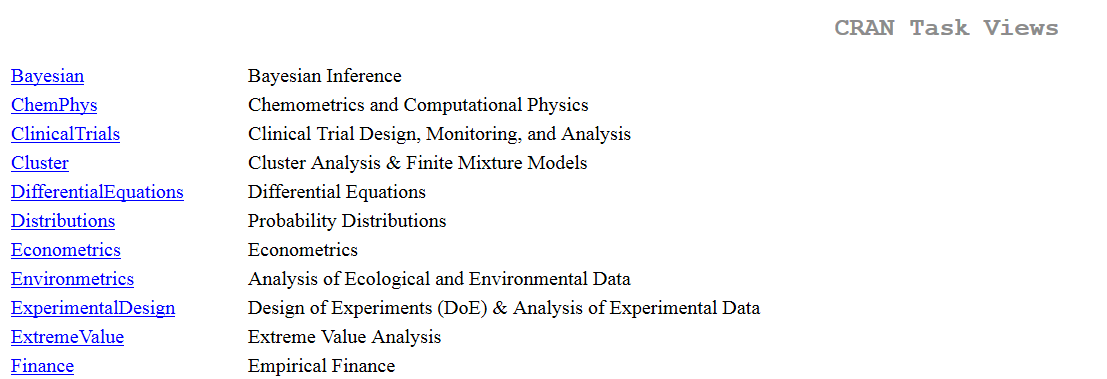
\includegraphics{./tex2pdf.956/add042645f04b28284c1b44301a5173fdf315965.png}

\end{block}

\end{frame}

\begin{frame}{Aufgabe - Zusatzpakete}

Gehen Sie auf \url{https://cran.r-project.org/} und suchen Sie in dem
Bereich, wo die Pakete vorgestellt werden, nach Paketen,\ldots{}

\begin{itemize}
\tightlist
\item
  die für die deskriptive Datenanalyse geeignet sind.
\item
  um Regressionen zu berechnen
\item
  um fremde Datensätze einzulesen (z.B. SPSS-Daten)
\item
  um mit großen Datenmengen umzugehen
\end{itemize}

\end{frame}

\begin{frame}{Datenimport}

\end{frame}

\begin{frame}{Datenimport}


\includegraphics{./tex2pdf.956/c6299486de2fc9d0f47deb7c7690d9756466e12d.png}

\end{frame}

\begin{frame}{Dateiformate in R}

\begin{itemize}
\tightlist
\item
  Von R werden quelloffene, nicht-proprietäre Formate bevorzugt
\item
  Es können aber auch Formate von anderen Statistik Software Paketen
  eingelesen werden
\item
  R-user speichern Objekte gerne in sog. Workspaces ab
\item
  Auch hier jedoch gilt: (fast) alles andere ist möglich
\end{itemize}

\end{frame}

\begin{frame}[fragile]{Formate - base package}

R unterstützt von Haus aus schon einige wichtige Formate:

\begin{itemize}
\tightlist
\item
  CSV (Comma Separated Values): \texttt{read.csv()}
\item
  FWF (Fixed With Format): \texttt{read.fwf()}
\item
  Tab-getrennte Werte: \texttt{read.delim()}
\end{itemize}

\end{frame}

\begin{frame}{Datenimport leicht gemacht mit Rstudio}

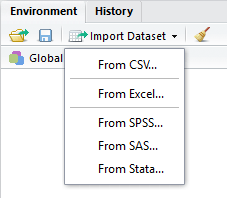
\includegraphics{./tex2pdf.956/746110b01ddf611ed8c07e15bb34f1ec7c4720f7.png}

\end{frame}

\begin{frame}[fragile]{Der Arbeitsspeicher}

So findet man heraus, in welchem Verzeichnis man sich gerade befindet

\begin{Shaded}
\begin{Highlighting}[]
\KeywordTok{getwd}\NormalTok{()}
\end{Highlighting}
\end{Shaded}

Und ändert dann den Pfad mit setwd()

\begin{Shaded}
\begin{Highlighting}[]
\KeywordTok{setwd}\NormalTok{(}\StringTok{"C:/"}\NormalTok{)}
\end{Highlighting}
\end{Shaded}

Man erzeugt ein Objekt in dem man den Pfad abspeichert:

\begin{Shaded}
\begin{Highlighting}[]
\NormalTok{main.path <-}\StringTok{ "C:/"} \CommentTok{# Beispiel für Windows}
\NormalTok{main.path <-}\StringTok{ "/users/Name/"} \CommentTok{# Beispiel für Mac}
\NormalTok{main.path <-}\StringTok{ "/home/user/"} \CommentTok{# Beispiel für Linux}
\end{Highlighting}
\end{Shaded}

Bei Windows ist es wichtig Slashs anstelle von Backslashs zu verwenden.

\end{frame}

\begin{frame}{Alternative - Arbeitsspeicher}

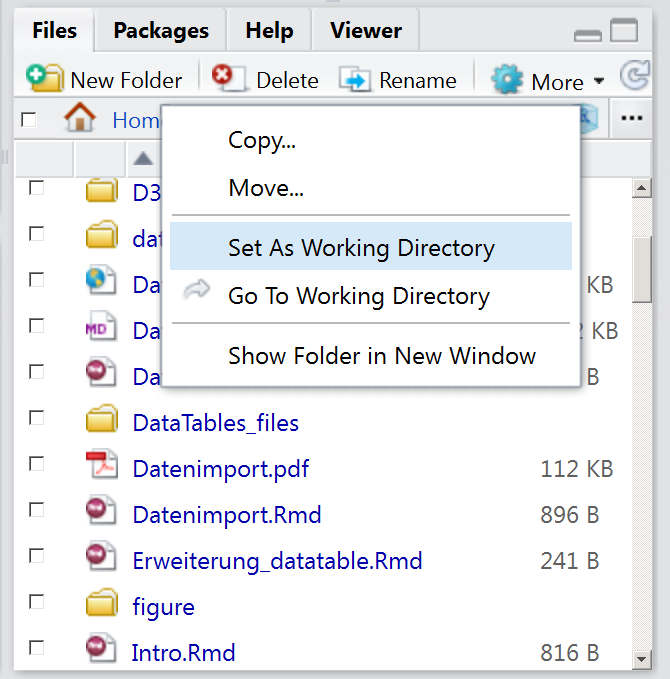
\includegraphics{./tex2pdf.956/f4ebbc3c67143aca8b1f90ded80bc3bfc7e2d639.png}

\end{frame}

\begin{frame}[fragile]{Import von Excel-Daten}

\begin{itemize}
\tightlist
\item
  \texttt{library(foreign)} ist für den Import von fremden Datenformaten
  nötig
\item
  Wenn Excel-Daten vorliegen - als .csv abspeichern
\item
  Dann kann \texttt{read.csv()} genutzt werden um die Daten einzulesen.
\item
  Bei Deutschen Daten kann es sein, dass man \texttt{read.csv2()} wegen
  der Komma-Separierung braucht.
\end{itemize}

\begin{Shaded}
\begin{Highlighting}[]
\KeywordTok{library}\NormalTok{(foreign)}
\NormalTok{?read.csv}
\NormalTok{?read.csv2}
\end{Highlighting}
\end{Shaded}

\end{frame}

\begin{frame}[fragile]{CSV Dateien einlesen}

Zunächst muss das Arbeitsverzeichnis gesetzt werden, in dem sich die
Daten befinden:

\begin{Shaded}
\begin{Highlighting}[]
\NormalTok{Dat <-}\StringTok{ }\KeywordTok{read.csv}\NormalTok{(}\StringTok{"schuldaten_export.csv"}\NormalTok{)}
\end{Highlighting}
\end{Shaded}

Wenn es sich um Deutsche Daten handelt:

\begin{Shaded}
\begin{Highlighting}[]
\NormalTok{Dat <-}\StringTok{ }\KeywordTok{read.csv2}\NormalTok{(}\StringTok{"schuldaten_export.csv"}\NormalTok{)}
\end{Highlighting}
\end{Shaded}

\end{frame}

\begin{frame}{CSV aus dem Web einladen}

\begin{itemize}
\tightlist
\item
  Datensatz:
\end{itemize}

\url{https://data.montgomerycountymd.gov/api/views/6rqk-pdub/rows.csv?accessType=DOWNLOAD}

\begin{itemize}
\tightlist
\item
  \href{https://support.rstudio.com/hc/en-us/articles/218611977-Importing-Data-with-RStudio}{Datenimport
  mit Rstudio}
\end{itemize}

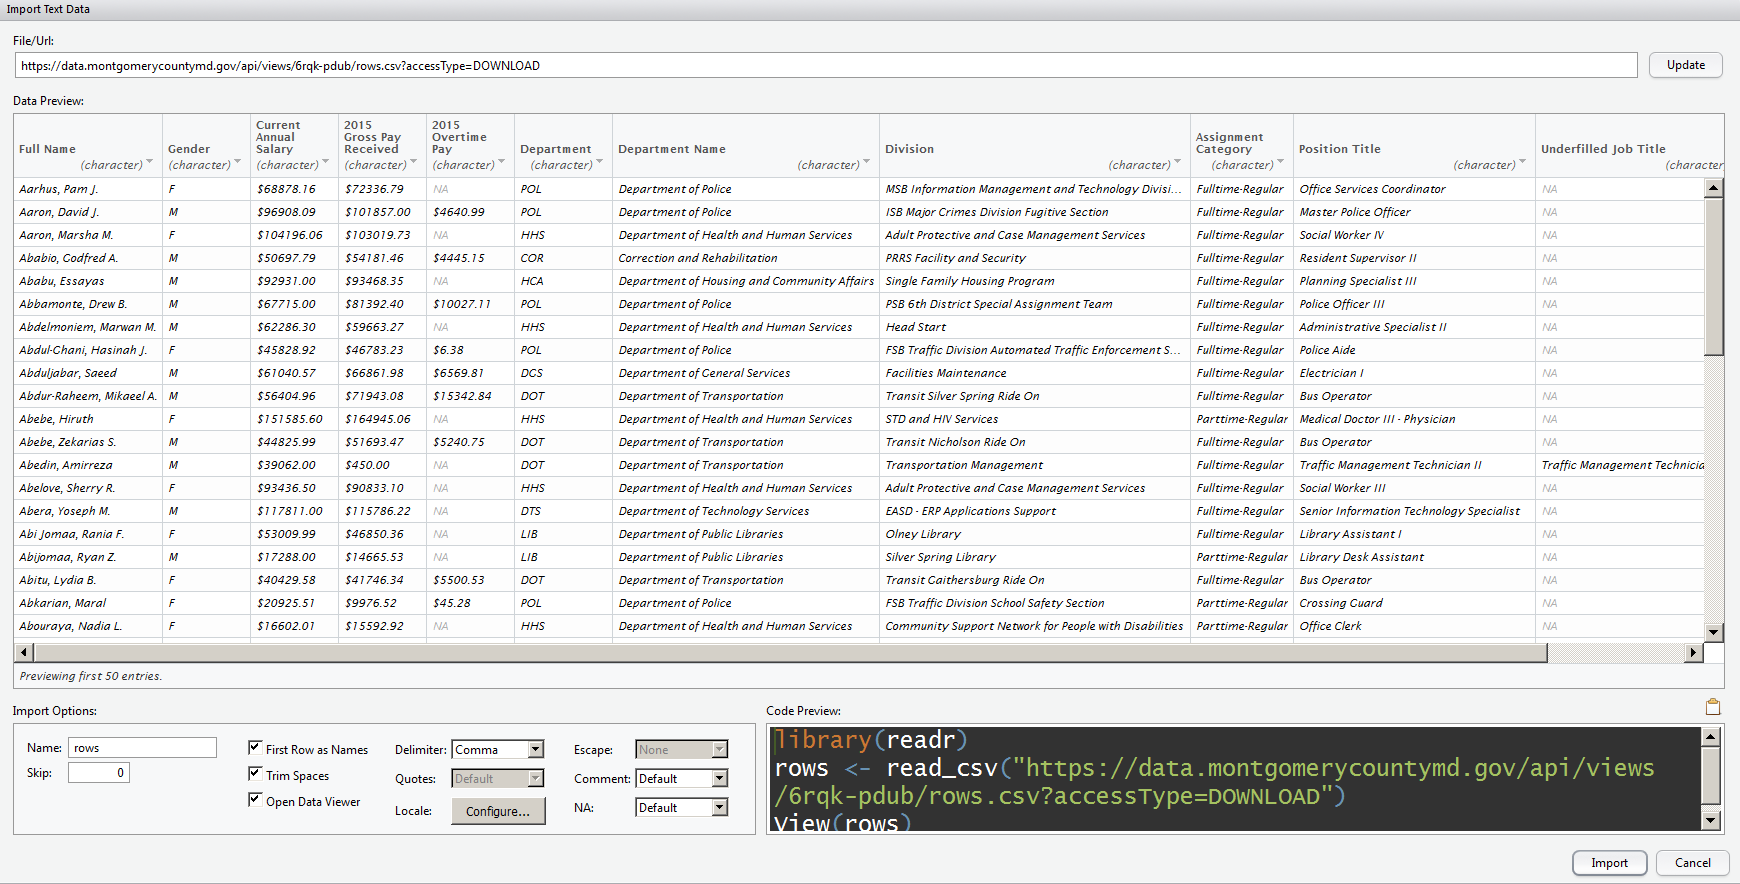
\includegraphics{./tex2pdf.956/74bec32bd4334be5ae8e5422ac2c166dd8414ddb.png}

\end{frame}

\begin{frame}[fragile]{Das Paket \texttt{readr}}

\begin{block}{Das Paket
\href{https://blog.rstudio.org/2015/10/28/readr-0-2-0/}{\texttt{readr}
(Rstudio Blogg)}}

\begin{Shaded}
\begin{Highlighting}[]
\KeywordTok{install.packages}\NormalTok{(}\StringTok{"readr"}\NormalTok{)}
\end{Highlighting}
\end{Shaded}

\begin{Shaded}
\begin{Highlighting}[]
\KeywordTok{library}\NormalTok{(readr)}
\end{Highlighting}
\end{Shaded}

\end{block}

\end{frame}

\begin{frame}[fragile]{Import von Excel-Daten}

\begin{itemize}
\tightlist
\item
  \texttt{library(readr)} ist für den Import von fremden Datenformaten
  hilfreich
\item
  Wenn Excel-Daten vorliegen - als .csv abspeichern
\end{itemize}

\begin{block}{Beispiel Weltkulturerbestätten}

\begin{Shaded}
\begin{Highlighting}[]
\NormalTok{url<-}\StringTok{"https://raw.githubusercontent.com/Japhilko/GeoData/master/2015/data/whcSites.csv"}

\NormalTok{whcSites <-}\StringTok{ }\KeywordTok{read.csv}\NormalTok{(url) }
\end{Highlighting}
\end{Shaded}

\end{block}

\end{frame}

\begin{frame}{Der Beispieldatensatz}

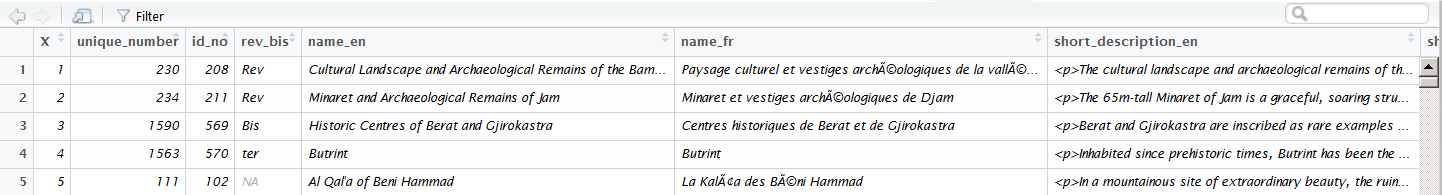
\includegraphics{./tex2pdf.956/2660e2345e9e67c6183dba09dc92fe1b26a231dc.png}

\end{frame}

\begin{frame}[fragile]{Das Paket \texttt{haven}}

\begin{quote}
Import and Export `SPSS', `Stata' and `SAS' Files
\end{quote}

\begin{Shaded}
\begin{Highlighting}[]
\KeywordTok{install.packages}\NormalTok{(}\StringTok{"haven"}\NormalTok{)}
\end{Highlighting}
\end{Shaded}

\begin{Shaded}
\begin{Highlighting}[]
\KeywordTok{library}\NormalTok{(haven)}
\end{Highlighting}
\end{Shaded}

\begin{itemize}
\tightlist
\item
  \href{https://blog.rstudio.org/2016/10/04/haven-1-0-0/}{Das R-Paket
  \texttt{haven} auf dem Rstudio Blogg}
\end{itemize}

\end{frame}

\begin{frame}[fragile]{SPSS Dateien einlesen}

\begin{itemize}
\tightlist
\item
  Zunächst muss wieder der Pfad zum Arbeitsverzeichnis angeben werden.
\item
  SPSS-Dateien können auch direkt aus dem Internet geladen werden:
\end{itemize}

\begin{Shaded}
\begin{Highlighting}[]
\KeywordTok{library}\NormalTok{(haven)}
\NormalTok{mtcars <-}\StringTok{ }\KeywordTok{read_sav}\NormalTok{(}
\StringTok{"https://github.com/Japhilko/RInterfaces/raw/master/}
\StringTok{data/mtcars.sav"}\NormalTok{)}
\end{Highlighting}
\end{Shaded}

\end{frame}

\begin{frame}[fragile]{\texttt{foreign} kann ebenfalls zum Import
genutzt werden}

\begin{Shaded}
\begin{Highlighting}[]
\KeywordTok{library}\NormalTok{(foreign)}
\NormalTok{link<-}\StringTok{ "http://www.statistik.at/web_de/static/}
\StringTok{mz_2013_sds_-_datensatz_080469.sav"}

\NormalTok{?read.spss}
\NormalTok{Dat <-}\StringTok{ }\KeywordTok{read.spss}\NormalTok{(link,}\DataTypeTok{to.data.frame=}\NormalTok{T)}
\end{Highlighting}
\end{Shaded}

\end{frame}

\begin{frame}[fragile]{stata Dateien einlesen}

\begin{Shaded}
\begin{Highlighting}[]
\KeywordTok{library}\NormalTok{(haven)}
\NormalTok{oecd <-}\StringTok{ }\KeywordTok{read_dta}\NormalTok{(}\StringTok{"https://github.com/Japhilko/IntroR/}
\StringTok{                 raw/master/2017/data/oecd.dta"}\NormalTok{)}
\end{Highlighting}
\end{Shaded}

\begin{itemize}
\tightlist
\item
  Einführung in Import mit R
  (\href{http://is-r.tumblr.com/post/37181850668/reading-writing-stata-dta-files-with-foreign}{is.R})
\end{itemize}

\end{frame}

\begin{frame}[fragile]{Das Paket \texttt{readstata13}}

\begin{block}{\emph{Import `Stata' Data Files}}

\begin{Shaded}
\begin{Highlighting}[]
\CommentTok{# install.packages("readstata13")}
\end{Highlighting}
\end{Shaded}

\begin{Shaded}
\begin{Highlighting}[]
\KeywordTok{library}\NormalTok{(readstata13)}
\NormalTok{?read.dta13}
\end{Highlighting}
\end{Shaded}

\end{block}

\end{frame}

\begin{frame}[fragile]{\href{https://cran.r-project.org/web/packages/rio/vignettes/rio.html}{Das
Paket \texttt{rio}}}

\begin{Shaded}
\begin{Highlighting}[]
\KeywordTok{install.packages}\NormalTok{(}\StringTok{"rio"}\NormalTok{)}
\end{Highlighting}
\end{Shaded}

\begin{Shaded}
\begin{Highlighting}[]
\KeywordTok{library}\NormalTok{(}\StringTok{"rio"}\NormalTok{)}
\NormalTok{x <-}\StringTok{ }\KeywordTok{import}\NormalTok{(}\StringTok{"mtcars.csv"}\NormalTok{)}
\NormalTok{y <-}\StringTok{ }\KeywordTok{import}\NormalTok{(}\StringTok{"mtcars.rds"}\NormalTok{)}
\NormalTok{z <-}\StringTok{ }\KeywordTok{import}\NormalTok{(}\StringTok{"mtcars.dta"}\NormalTok{)}
\end{Highlighting}
\end{Shaded}

\begin{itemize}
\tightlist
\item
  \href{https://cran.r-project.org/web/packages/rio/README.html}{rio: A
  Swiss-Army Knife for Data I/O}
\end{itemize}

\end{frame}

\begin{frame}[fragile]{\href{https://cran.r-project.org/web/packages/Rcmdr/index.html}{Weitere
Alternative Rcmdr}}

\begin{Shaded}
\begin{Highlighting}[]
\KeywordTok{install.packages}\NormalTok{(}\StringTok{"Rcmdr"}\NormalTok{)}
\end{Highlighting}
\end{Shaded}

\begin{itemize}
\tightlist
\item
  \href{http://www.rcommander.com/}{Funktioniert auch mit Rstudio}
\end{itemize}

\begin{Shaded}
\begin{Highlighting}[]
\KeywordTok{library}\NormalTok{(Rcmdr)}
\end{Highlighting}
\end{Shaded}

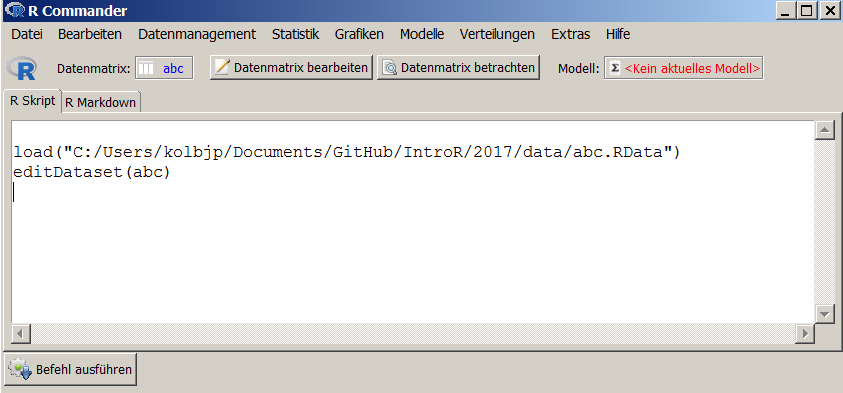
\includegraphics{./tex2pdf.956/7fc6300bc58e78aaaf7433492aaeaa8d1319075c.png}

\end{frame}

\begin{frame}{Die Gesis Panel Daten}


\includegraphics{./tex2pdf.956/5e78f32f301eb9cbc23cee28d482621ebc199870.jpg}

\begin{itemize}
\item
  \href{http://www.gesis.org/gesis-panel/data/gesis-panel-campus-file/}{Gesis
  Panel Campus File}
\item
  \href{https://dbk.gesis.org/dbksearch/SDesc2.asp?ll=10\&notabs=\&af=\&nf=\&search=gesis\%20panel\&search2=\&db=D\&no=5665}{Codebuch
  für die Gesis Panel Daten im DBK}
\end{itemize}

\end{frame}

\begin{frame}[fragile]{Gesis Panel Daten einlesen}

\begin{Shaded}
\begin{Highlighting}[]
\KeywordTok{library}\NormalTok{(readstata13)}
\NormalTok{dat <-}\StringTok{ }\KeywordTok{read.dta13}\NormalTok{(}\StringTok{"ZA5666_v1-0-0_Stata14.dta"}\NormalTok{)}
\NormalTok{attdat <-}\StringTok{ }\KeywordTok{attributes}\NormalTok{(dat)}
\NormalTok{varlabs <-}\StringTok{ }\KeywordTok{data.frame}\NormalTok{(}\KeywordTok{colnames}\NormalTok{(dat),attdat$var.labels)}
\NormalTok{attdat$var.labels}
\end{Highlighting}
\end{Shaded}

\begin{verbatim}
##  [1] "Personen ID - Campus File"                    
##  [2] "Studiennummer des Archivs"                    
##  [3] "Versionskennung und -datum des Archivs"       
##  [4] "doi"                                          
##  [5] "Zufriedenheit Leben in Wohnort"               
##  [6] "Zufriedenheit Leben in Deutschland"           
##  [7] "Zufriedenheit Leben allgemein"                
##  [8] "Vertrauen: Allgemeines Vertrauen"             
##  [9] "Vertrauen: Kein Verlass"                      
## [10] "Vertrauen: Vorsichtig sein bei Fremden"       
## [11] "Lebensstandard junge Generation"              
## [12] "Freizeit Häufigkeit: Bücher lesen"            
## [13] "Freizeit Häufigkeit: Zeitschriften lesen"     
## [14] "Freizeit Häufigkeit: Zeitung lesen"           
## [15] "Freizeit Häufigkeit: Musik hören"             
## [16] "Freizeit Häufigkeit: Fernsehen"               
## [17] "Freizeit Häufigkeit: Computer"                
## [18] "Freizeit Häufigkeit: Spazieren gehen, Wandern"
## [19] "Freizeit Häufigkeit: Sport"                   
## [20] "Private Internetnutzung"
\end{verbatim}

\end{frame}

\begin{frame}{Gesis Panel - Variablen Labels}

\begin{longtable}[]{@{}ll@{}}
\toprule
colnames.dat. & attdat.var.labels\tabularnewline
\midrule
\endhead
z000001z & Personen ID - Campus File\tabularnewline
z000002z & Studiennummer des Archivs\tabularnewline
z000003z & Versionskennung und -datum des Archivs\tabularnewline
z000005z & doi\tabularnewline
a11c019a & Zufriedenheit Leben in Wohnort\tabularnewline
a11c020a & Zufriedenheit Leben in Deutschland\tabularnewline
\bottomrule
\end{longtable}

\end{frame}

\begin{frame}[fragile]{Aufgabe}

\begin{itemize}
\tightlist
\item
  Gehen Sie auf meine Github Seite
\end{itemize}

\url{https://github.com/Japhilko/RSocialScience/tree/master/data}

\begin{itemize}
\tightlist
\item
  Importieren Sie den Datensatz \texttt{GPanel.dta}
\end{itemize}

\end{frame}

\begin{frame}{Datenaufbereitung}

\end{frame}

\begin{frame}[fragile]{Data Frames}

\begin{block}{Beispieldaten einlesen:}

\begin{Shaded}
\begin{Highlighting}[]
\KeywordTok{library}\NormalTok{(foreign)}
\NormalTok{dat<-}\KeywordTok{read.dta}\NormalTok{(}\StringTok{"https://github.com/Japhilko/RSocialScience/}
\StringTok{              raw/master/data/GPanel.dta"}\NormalTok{)}
\end{Highlighting}
\end{Shaded}

\begin{itemize}
\tightlist
\item
  Auf dem Github Verzeichnis liegt eine verkleinerte Version des Campus
  Files.
\item
  Alle Operationen sollten aber auch mit dem größeren Datensatz
  funktionieren
\end{itemize}

\end{block}

\end{frame}

\begin{frame}{Übersicht mittels Rstudio}

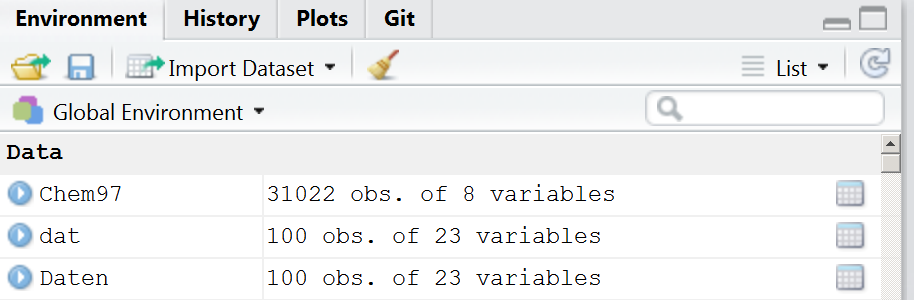
\includegraphics{./tex2pdf.956/46e5b1121194c894f424f27d4be84216d8efec9e.png}

\end{frame}

\begin{frame}{\href{https://support.rstudio.com/hc/en-us/articles/205175388-Using-the-Data-Viewer}{Den
Datensatz anschauen}}

\begin{block}{Die Daten filtern}

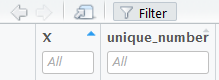
\includegraphics{./tex2pdf.956/ede672ed41a6acc2a56fb75762d0f0d2d7529ef2.png}

\end{block}

\end{frame}

\begin{frame}{Daten filtern}

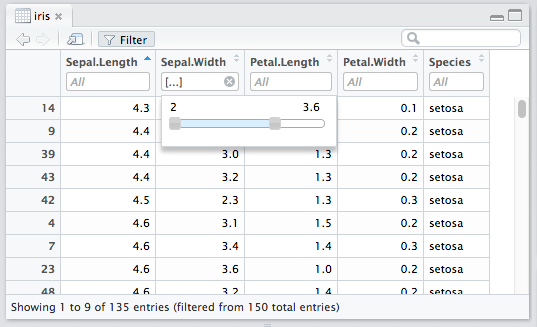
\includegraphics{./tex2pdf.956/35dc4a58b2ab7a9ea8377ea6129b7c5fc8d08014.png}

\end{frame}

\begin{frame}[fragile]{Struktur des Datensatzes}

\begin{block}{Der Datentyp}

\begin{Shaded}
\begin{Highlighting}[]
\KeywordTok{typeof}\NormalTok{(dat)}
\end{Highlighting}
\end{Shaded}

\begin{verbatim}
## [1] "list"
\end{verbatim}

\end{block}

\begin{block}{\href{https://stats.stackexchange.com/questions/11551/is-there-a-good-browser-viewer-to-see-an-r-dataset-rda-file}{Die
Funktion \texttt{glimpse} im Paket \texttt{dplyr}}}

\begin{Shaded}
\begin{Highlighting}[]
\KeywordTok{library}\NormalTok{(dplyr)}
\KeywordTok{glimpse}\NormalTok{(dat)}
\end{Highlighting}
\end{Shaded}

\begin{verbatim}
## Observations: 100
## Variables: 23
## $ a11c019a <fctr> Eher zufrieden, Sehr zufrieden, Eher zufrieden, Eher...
## $ a11c020a <fctr> Weder zufrieden noch unzufrieden, Eher unzufrieden, ...
## $ a11c021a <fctr> Sehr zufrieden, Eher unzufrieden, Eher unzufrieden, ...
## $ a11c022a <fctr> Stimme eher nicht zu, Stimme eher nicht zu, Stimme e...
## $ a11c023a <fctr> Stimme eher zu, Stimme eher zu, Stimme eher nicht zu...
## $ a11c024a <fctr> Stimme eher zu, Stimme voll und ganz zu, Stimme eher...
## $ a11c025a <fctr> Eher niedrigeren Lebensstandard, Eher niedrigeren Le...
## $ a11c026a <fctr> Seltener, Mehrmals die Woche, Täglich, Täglich, Tägl...
## $ a11c027a <fctr> Mehrmals die Woche, Mindestens einmal im Monat, Mehr...
## $ a11c028a <fctr> Täglich, Täglich, Nie, Täglich, Täglich, Täglich, Tä...
## $ a11c029a <fctr> Täglich, Täglich, Täglich, Täglich, Täglich, Nie, Tä...
## $ a11c030a <fctr> Täglich, Täglich, Mehrmals die Woche, Mehrmals die W...
## $ a11c031a <fctr> Seltener, Mindestens einmal im Monat, Täglich, Mehrm...
## $ a11c032a <fctr> Täglich, Mehrmals im Monat, Mehrmals die Woche, Selt...
## $ a11c033a <fctr> Täglich, Seltener, Mehrmals im Monat, Mehrmals die W...
## $ a11c034a <fctr> Ja, nutzt Internet für private Zwecke, Ja, nutzt Int...
## $ bazq020a <chr> "-33", "30", "35", "-33", "23", "15", "15", "15-20", ...
## $ a11d054a <fctr> Männlich, Männlich, Männlich, Männlich, Männlich, We...
## $ a11d056z <fctr> 45 bis unter 50 Jahre, 50 bis unter 55 Jahre, 20 bis...
## $ a11d092a <fctr> Angestellte(r), Missing by filter, Missing by filter...
## $ a11c100a <fctr> 5 .., 6 .., 6 .., 4 .., 6 .., 7 Sehr wichtig, 7 Sehr...
## $ a11c111a <fctr> Missing by design, Missing by design, Missing by des...
## $ a11c109a <fctr> Missing by design, Missing by design, Missing by des...
\end{verbatim}

\end{block}

\end{frame}

\begin{frame}[fragile]{In Dataframe übertragen}

Die Vektoren (von \texttt{dat}) zu einem data.frame verbinden:

\begin{Shaded}
\begin{Highlighting}[]
\NormalTok{Daten <-}\StringTok{ }\KeywordTok{data.frame}\NormalTok{(dat)}
\end{Highlighting}
\end{Shaded}

Anzahl der Zeilen/Spalten herausfinden

\begin{Shaded}
\begin{Highlighting}[]
\KeywordTok{nrow}\NormalTok{(Daten) }\CommentTok{# Zeilen}
\end{Highlighting}
\end{Shaded}

\begin{verbatim}
## [1] 100
\end{verbatim}

\begin{Shaded}
\begin{Highlighting}[]
\KeywordTok{ncol}\NormalTok{(Daten) }\CommentTok{# Spalten}
\end{Highlighting}
\end{Shaded}

\begin{verbatim}
## [1] 23
\end{verbatim}

\end{frame}

\begin{frame}[fragile]{Die Daten in der Console anschauen}

\begin{block}{Die ersten Zeilen anschauen}

\begin{Shaded}
\begin{Highlighting}[]
\KeywordTok{head}\NormalTok{(Daten)}
\end{Highlighting}
\end{Shaded}

\end{block}

\begin{block}{Die letzten Zeilen anschauen}

\begin{Shaded}
\begin{Highlighting}[]
\KeywordTok{tail}\NormalTok{(Daten)}
\end{Highlighting}
\end{Shaded}

\end{block}

\end{frame}

\begin{frame}[fragile]{Indizieren}

Indizieren eines dataframe:

\begin{Shaded}
\begin{Highlighting}[]
\NormalTok{Daten[}\DecValTok{1}\NormalTok{,}\DecValTok{1}\NormalTok{]}
\end{Highlighting}
\end{Shaded}

\begin{verbatim}
## [1] Eher zufrieden
## 7 Levels: Item nonresponse Sehr zufrieden ... Weiß nicht
\end{verbatim}

\begin{Shaded}
\begin{Highlighting}[]
\NormalTok{Daten[}\DecValTok{2}\NormalTok{,]}
\end{Highlighting}
\end{Shaded}

\begin{verbatim}
##         a11c019a         a11c020a         a11c021a             a11c022a
## 2 Sehr zufrieden Eher unzufrieden Eher unzufrieden Stimme eher nicht zu
##         a11c023a                a11c024a                        a11c025a
## 2 Stimme eher zu Stimme voll und ganz zu Eher niedrigeren Lebensstandard
##             a11c026a                   a11c027a a11c028a a11c029a a11c030a
## 2 Mehrmals die Woche Mindestens einmal im Monat  Täglich  Täglich  Täglich
##                     a11c031a          a11c032a a11c033a
## 2 Mindestens einmal im Monat Mehrmals im Monat Seltener
##                                a11c034a bazq020a a11d054a
## 2 Ja, nutzt Internet für private Zwecke       30 Männlich
##                a11d056z          a11d092a a11c100a          a11c111a
## 2 50 bis unter 55 Jahre Missing by filter     6 .. Missing by design
##            a11c109a
## 2 Missing by design
\end{verbatim}

\begin{Shaded}
\begin{Highlighting}[]
\NormalTok{Daten[,}\DecValTok{1}\NormalTok{]}
\end{Highlighting}
\end{Shaded}

\begin{verbatim}
##   [1] Eher zufrieden                   Sehr zufrieden                  
##   [3] Eher zufrieden                   Eher zufrieden                  
##   [5] Eher zufrieden                   Sehr zufrieden                  
##   [7] Eher zufrieden                   Eher zufrieden                  
##   [9] Sehr zufrieden                   Sehr zufrieden                  
##  [11] Eher zufrieden                   Sehr zufrieden                  
##  [13] Eher zufrieden                   Sehr zufrieden                  
##  [15] Sehr zufrieden                   Sehr zufrieden                  
##  [17] Weder zufrieden noch unzufrieden Eher zufrieden                  
##  [19] Sehr zufrieden                   Eher zufrieden                  
##  [21] Sehr zufrieden                   Sehr zufrieden                  
##  [23] Sehr zufrieden                   Sehr zufrieden                  
##  [25] Sehr zufrieden                   Weder zufrieden noch unzufrieden
##  [27] Eher unzufrieden                 Weder zufrieden noch unzufrieden
##  [29] Sehr zufrieden                   Eher zufrieden                  
##  [31] Sehr zufrieden                   Weder zufrieden noch unzufrieden
##  [33] Eher zufrieden                   Eher zufrieden                  
##  [35] Sehr zufrieden                   Eher zufrieden                  
##  [37] Eher zufrieden                   Sehr zufrieden                  
##  [39] Eher zufrieden                   Eher zufrieden                  
##  [41] Sehr zufrieden                   Sehr zufrieden                  
##  [43] Eher zufrieden                   Sehr zufrieden                  
##  [45] Sehr zufrieden                   Eher zufrieden                  
##  [47] Sehr zufrieden                   Eher zufrieden                  
##  [49] Sehr zufrieden                   Sehr zufrieden                  
##  [51] Eher zufrieden                   Weder zufrieden noch unzufrieden
##  [53] Eher zufrieden                   Eher zufrieden                  
##  [55] Sehr zufrieden                   Eher zufrieden                  
##  [57] Sehr zufrieden                   Sehr zufrieden                  
##  [59] Weder zufrieden noch unzufrieden Sehr zufrieden                  
##  [61] Sehr zufrieden                   Sehr unzufrieden                
##  [63] Sehr zufrieden                   Sehr zufrieden                  
##  [65] Eher zufrieden                   Eher zufrieden                  
##  [67] Sehr zufrieden                   Weder zufrieden noch unzufrieden
##  [69] Sehr zufrieden                   Eher zufrieden                  
##  [71] Eher zufrieden                   Sehr zufrieden                  
##  [73] Eher zufrieden                   Eher zufrieden                  
##  [75] Eher zufrieden                   Weder zufrieden noch unzufrieden
##  [77] Eher zufrieden                   Sehr zufrieden                  
##  [79] Sehr zufrieden                   Sehr zufrieden                  
##  [81] Eher zufrieden                   Eher zufrieden                  
##  [83] Sehr zufrieden                   Weder zufrieden noch unzufrieden
##  [85] Eher zufrieden                   Sehr zufrieden                  
##  [87] Sehr zufrieden                   Eher zufrieden                  
##  [89] Eher zufrieden                   Eher zufrieden                  
##  [91] Sehr zufrieden                   Eher zufrieden                  
##  [93] Eher zufrieden                   Sehr zufrieden                  
##  [95] Eher unzufrieden                 Sehr zufrieden                  
##  [97] Eher zufrieden                   Eher zufrieden                  
##  [99] Sehr zufrieden                   Eher unzufrieden                
## 7 Levels: Item nonresponse Sehr zufrieden ... Weiß nicht
\end{verbatim}

\begin{verbatim}
## [1] Eher zufrieden Sehr zufrieden Eher zufrieden Eher zufrieden
## [5] Eher zufrieden Sehr zufrieden
## 7 Levels: Item nonresponse Sehr zufrieden ... Weiß nicht
\end{verbatim}

\begin{Shaded}
\begin{Highlighting}[]
\NormalTok{Daten[,}\DecValTok{1}\NormalTok{:}\DecValTok{2}\NormalTok{]}
\end{Highlighting}
\end{Shaded}

\begin{verbatim}
##                             a11c019a                         a11c020a
## 1                     Eher zufrieden Weder zufrieden noch unzufrieden
## 2                     Sehr zufrieden                 Eher unzufrieden
## 3                     Eher zufrieden                   Sehr zufrieden
## 4                     Eher zufrieden                   Sehr zufrieden
## 5                     Eher zufrieden                   Eher zufrieden
## 6                     Sehr zufrieden                   Eher zufrieden
## 7                     Eher zufrieden                   Eher zufrieden
## 8                     Eher zufrieden                   Eher zufrieden
## 9                     Sehr zufrieden                   Eher zufrieden
## 10                    Sehr zufrieden                   Sehr zufrieden
## 11                    Eher zufrieden                   Eher zufrieden
## 12                    Sehr zufrieden                   Eher zufrieden
## 13                    Eher zufrieden Weder zufrieden noch unzufrieden
## 14                    Sehr zufrieden                   Sehr zufrieden
## 15                    Sehr zufrieden                   Sehr zufrieden
## 16                    Sehr zufrieden                   Sehr zufrieden
## 17  Weder zufrieden noch unzufrieden                 Eher unzufrieden
## 18                    Eher zufrieden                   Sehr zufrieden
## 19                    Sehr zufrieden                   Sehr zufrieden
## 20                    Eher zufrieden                   Eher zufrieden
## 21                    Sehr zufrieden                   Sehr zufrieden
## 22                    Sehr zufrieden                   Sehr zufrieden
## 23                    Sehr zufrieden                   Eher zufrieden
## 24                    Sehr zufrieden                   Sehr zufrieden
## 25                    Sehr zufrieden                   Sehr zufrieden
## 26  Weder zufrieden noch unzufrieden                   Eher zufrieden
## 27                  Eher unzufrieden                   Eher zufrieden
## 28  Weder zufrieden noch unzufrieden Weder zufrieden noch unzufrieden
## 29                    Sehr zufrieden                   Sehr zufrieden
## 30                    Eher zufrieden Weder zufrieden noch unzufrieden
## 31                    Sehr zufrieden                   Eher zufrieden
## 32  Weder zufrieden noch unzufrieden                   Eher zufrieden
## 33                    Eher zufrieden                   Sehr zufrieden
## 34                    Eher zufrieden                   Sehr zufrieden
## 35                    Sehr zufrieden                   Eher zufrieden
## 36                    Eher zufrieden                   Eher zufrieden
## 37                    Eher zufrieden                   Eher zufrieden
## 38                    Sehr zufrieden                   Eher zufrieden
## 39                    Eher zufrieden                   Eher zufrieden
## 40                    Eher zufrieden                   Sehr zufrieden
## 41                    Sehr zufrieden                   Eher zufrieden
## 42                    Sehr zufrieden                   Eher zufrieden
## 43                    Eher zufrieden                 Eher unzufrieden
## 44                    Sehr zufrieden                   Eher zufrieden
## 45                    Sehr zufrieden                   Sehr zufrieden
## 46                    Eher zufrieden                   Sehr zufrieden
## 47                    Sehr zufrieden                   Eher zufrieden
## 48                    Eher zufrieden                   Eher zufrieden
## 49                    Sehr zufrieden                   Sehr zufrieden
## 50                    Sehr zufrieden                   Eher zufrieden
## 51                    Eher zufrieden                   Eher zufrieden
## 52  Weder zufrieden noch unzufrieden                   Eher zufrieden
## 53                    Eher zufrieden                   Eher zufrieden
## 54                    Eher zufrieden                   Eher zufrieden
## 55                    Sehr zufrieden                   Sehr zufrieden
## 56                    Eher zufrieden                   Eher zufrieden
## 57                    Sehr zufrieden                   Eher zufrieden
## 58                    Sehr zufrieden                   Sehr zufrieden
## 59  Weder zufrieden noch unzufrieden                   Eher zufrieden
## 60                    Sehr zufrieden                   Eher zufrieden
## 61                    Sehr zufrieden                   Eher zufrieden
## 62                  Sehr unzufrieden                 Sehr unzufrieden
## 63                    Sehr zufrieden                   Eher zufrieden
## 64                    Sehr zufrieden                   Sehr zufrieden
## 65                    Eher zufrieden                   Eher zufrieden
## 66                    Eher zufrieden                   Eher zufrieden
## 67                    Sehr zufrieden                   Eher zufrieden
## 68  Weder zufrieden noch unzufrieden                 Sehr unzufrieden
## 69                    Sehr zufrieden                   Sehr zufrieden
## 70                    Eher zufrieden                 Eher unzufrieden
## 71                    Eher zufrieden                   Eher zufrieden
## 72                    Sehr zufrieden                   Sehr zufrieden
## 73                    Eher zufrieden                 Sehr unzufrieden
## 74                    Eher zufrieden                   Eher zufrieden
## 75                    Eher zufrieden                   Sehr zufrieden
## 76  Weder zufrieden noch unzufrieden                   Sehr zufrieden
## 77                    Eher zufrieden Weder zufrieden noch unzufrieden
## 78                    Sehr zufrieden                   Eher zufrieden
## 79                    Sehr zufrieden                   Sehr zufrieden
## 80                    Sehr zufrieden                   Sehr zufrieden
## 81                    Eher zufrieden Weder zufrieden noch unzufrieden
## 82                    Eher zufrieden                   Eher zufrieden
## 83                    Sehr zufrieden                   Sehr zufrieden
## 84  Weder zufrieden noch unzufrieden Weder zufrieden noch unzufrieden
## 85                    Eher zufrieden Weder zufrieden noch unzufrieden
## 86                    Sehr zufrieden                   Eher zufrieden
## 87                    Sehr zufrieden                   Eher zufrieden
## 88                    Eher zufrieden                   Eher zufrieden
## 89                    Eher zufrieden                   Eher zufrieden
## 90                    Eher zufrieden                   Eher zufrieden
## 91                    Sehr zufrieden                   Sehr zufrieden
## 92                    Eher zufrieden                   Eher zufrieden
## 93                    Eher zufrieden                   Sehr zufrieden
## 94                    Sehr zufrieden                   Sehr zufrieden
## 95                  Eher unzufrieden                   Eher zufrieden
## 96                    Sehr zufrieden                   Eher zufrieden
## 97                    Eher zufrieden                   Eher zufrieden
## 98                    Eher zufrieden                   Sehr zufrieden
## 99                    Sehr zufrieden                   Eher zufrieden
## 100                 Eher unzufrieden                   Sehr zufrieden
\end{verbatim}

\end{frame}

\begin{frame}[fragile]{Operatoren um Subset für Datensatz zu bekommen}

Diese Operatoren eignen sich gut um Datensätze einzuschränken

\begin{Shaded}
\begin{Highlighting}[]
\NormalTok{Dauer <-}\StringTok{ }\KeywordTok{as.numeric}\NormalTok{(Daten$bazq020a)}
\end{Highlighting}
\end{Shaded}

\begin{verbatim}
## Warning: NAs durch Umwandlung erzeugt
\end{verbatim}

\begin{Shaded}
\begin{Highlighting}[]
\KeywordTok{head}\NormalTok{(Daten[Dauer>}\DecValTok{20}\NormalTok{,])}
\end{Highlighting}
\end{Shaded}

\begin{verbatim}
##          a11c019a         a11c020a         a11c021a             a11c022a
## 2  Sehr zufrieden Eher unzufrieden Eher unzufrieden Stimme eher nicht zu
## 3  Eher zufrieden   Sehr zufrieden Eher unzufrieden Stimme eher nicht zu
## 5  Eher zufrieden   Eher zufrieden   Eher zufrieden       Stimme eher zu
## NA           <NA>             <NA>             <NA>                 <NA>
## 9  Sehr zufrieden   Eher zufrieden   Sehr zufrieden       Stimme eher zu
## 15 Sehr zufrieden   Sehr zufrieden   Sehr zufrieden       Stimme eher zu
##                a11c023a                a11c024a
## 2        Stimme eher zu Stimme voll und ganz zu
## 3  Stimme eher nicht zu          Stimme eher zu
## 5        Stimme eher zu          Stimme eher zu
## NA                 <NA>                    <NA>
## 9  Stimme eher nicht zu Stimme voll und ganz zu
## 15 Stimme eher nicht zu    Stimme eher nicht zu
##                           a11c025a           a11c026a
## 2  Eher niedrigeren Lebensstandard Mehrmals die Woche
## 3         Denselben Lebensstandard            Täglich
## 5         Denselben Lebensstandard            Täglich
## NA                            <NA>               <NA>
## 9         Denselben Lebensstandard                Nie
## 15        Denselben Lebensstandard                Nie
##                      a11c027a a11c028a          a11c029a
## 2  Mindestens einmal im Monat  Täglich           Täglich
## 3           Mehrmals im Monat      Nie           Täglich
## 5          Mehrmals die Woche  Täglich           Täglich
## NA                       <NA>     <NA>              <NA>
## 9                    Seltener  Täglich Mehrmals im Monat
## 15                    Täglich  Täglich           Täglich
##              a11c030a                   a11c031a           a11c032a
## 2             Täglich Mindestens einmal im Monat  Mehrmals im Monat
## 3  Mehrmals die Woche                    Täglich Mehrmals die Woche
## 5             Täglich         Mehrmals die Woche Mehrmals die Woche
## NA               <NA>                       <NA>               <NA>
## 9             Täglich                    Täglich           Seltener
## 15            Täglich                    Täglich  Mehrmals im Monat
##                      a11c033a                              a11c034a
## 2                    Seltener Ja, nutzt Internet für private Zwecke
## 3           Mehrmals im Monat Ja, nutzt Internet für private Zwecke
## 5  Mindestens einmal im Monat Ja, nutzt Internet für private Zwecke
## NA                       <NA>                                  <NA>
## 9           Mehrmals im Monat Ja, nutzt Internet für private Zwecke
## 15          Mehrmals im Monat Ja, nutzt Internet für private Zwecke
##    bazq020a a11d054a              a11d056z          a11d092a
## 2        30 Männlich 50 bis unter 55 Jahre Missing by filter
## 3        35 Männlich 20 bis unter 25 Jahre Missing by filter
## 5        23 Männlich 65 bis unter 70 Jahre Missing by filter
## NA     <NA>     <NA>                  <NA>              <NA>
## 9        25 Männlich 50 bis unter 55 Jahre    Angestellte(r)
## 15       25 Männlich 45 bis unter 50 Jahre    Angestellte(r)
##          a11c100a          a11c111a          a11c109a
## 2            6 .. Missing by design Missing by design
## 3            6 .. Missing by design Missing by design
## 5            6 .. Missing by design Missing by design
## NA           <NA>              <NA>              <NA>
## 9            5 .. Missing by design Missing by design
## 15 7 Sehr wichtig Missing by design Missing by design
\end{verbatim}

\end{frame}

\begin{frame}[fragile]{Einschränken mit dem Paket \texttt{tidyverse}}

\begin{itemize}
\tightlist
\item
  einfacher geht es mit dem Paket \texttt{tidyverse}
\end{itemize}

\begin{Shaded}
\begin{Highlighting}[]
\KeywordTok{library}\NormalTok{(tidyverse)}
\KeywordTok{filter}\NormalTok{(Daten, Dauer>}\DecValTok{20}\NormalTok{)}
\end{Highlighting}
\end{Shaded}

\begin{verbatim}
##                            a11c019a                         a11c020a
## 1                    Sehr zufrieden                 Eher unzufrieden
## 2                    Eher zufrieden                   Sehr zufrieden
## 3                    Eher zufrieden                   Eher zufrieden
## 4                    Sehr zufrieden                   Eher zufrieden
## 5                    Sehr zufrieden                   Sehr zufrieden
## 6                    Eher zufrieden                   Sehr zufrieden
## 7                    Sehr zufrieden                   Sehr zufrieden
## 8                    Sehr zufrieden                   Sehr zufrieden
## 9                    Eher zufrieden                   Eher zufrieden
## 10                   Sehr zufrieden                   Eher zufrieden
## 11                   Eher zufrieden                   Eher zufrieden
## 12                   Sehr zufrieden                   Sehr zufrieden
## 13                   Sehr zufrieden                   Eher zufrieden
## 14                   Sehr zufrieden                   Sehr zufrieden
## 15                   Eher zufrieden                   Eher zufrieden
## 16 Weder zufrieden noch unzufrieden                   Sehr zufrieden
## 17                   Sehr zufrieden                   Sehr zufrieden
## 18                   Eher zufrieden Weder zufrieden noch unzufrieden
## 19                 Eher unzufrieden                   Eher zufrieden
##            a11c021a                a11c022a                  a11c023a
## 1  Eher unzufrieden    Stimme eher nicht zu            Stimme eher zu
## 2  Eher unzufrieden    Stimme eher nicht zu      Stimme eher nicht zu
## 3    Eher zufrieden          Stimme eher zu            Stimme eher zu
## 4    Sehr zufrieden          Stimme eher zu      Stimme eher nicht zu
## 5    Sehr zufrieden          Stimme eher zu      Stimme eher nicht zu
## 6  Eher unzufrieden          Stimme eher zu      Stimme eher nicht zu
## 7    Sehr zufrieden    Stimme eher nicht zu      Stimme eher nicht zu
## 8    Sehr zufrieden          Stimme eher zu      Stimme eher nicht zu
## 9    Eher zufrieden    Stimme eher nicht zu      Stimme eher nicht zu
## 10   Sehr zufrieden          Stimme eher zu      Stimme eher nicht zu
## 11   Sehr zufrieden    Stimme eher nicht zu Stimme überhaupt nicht zu
## 12   Sehr zufrieden    Stimme eher nicht zu      Stimme eher nicht zu
## 13   Sehr zufrieden Stimme voll und ganz zu      Stimme eher nicht zu
## 14   Sehr zufrieden          Stimme eher zu      Stimme eher nicht zu
## 15   Eher zufrieden          Stimme eher zu      Stimme eher nicht zu
## 16   Eher zufrieden          Stimme eher zu Stimme überhaupt nicht zu
## 17   Eher zufrieden          Stimme eher zu      Stimme eher nicht zu
## 18   Eher zufrieden    Stimme eher nicht zu            Stimme eher zu
## 19   Eher zufrieden    Stimme eher nicht zu   Stimme voll und ganz zu
##                   a11c024a                        a11c025a
## 1  Stimme voll und ganz zu Eher niedrigeren Lebensstandard
## 2           Stimme eher zu        Denselben Lebensstandard
## 3           Stimme eher zu        Denselben Lebensstandard
## 4  Stimme voll und ganz zu        Denselben Lebensstandard
## 5     Stimme eher nicht zu        Denselben Lebensstandard
## 6           Stimme eher zu Eher niedrigeren Lebensstandard
## 7  Stimme voll und ganz zu Eher niedrigeren Lebensstandard
## 8           Stimme eher zu Eher niedrigeren Lebensstandard
## 9           Stimme eher zu Eher niedrigeren Lebensstandard
## 10          Stimme eher zu     Eher höheren Lebensstandard
## 11 Stimme voll und ganz zu Eher niedrigeren Lebensstandard
## 12 Stimme voll und ganz zu Eher niedrigeren Lebensstandard
## 13          Stimme eher zu     Eher höheren Lebensstandard
## 14          Stimme eher zu Eher niedrigeren Lebensstandard
## 15          Stimme eher zu     Eher höheren Lebensstandard
## 16          Stimme eher zu        Denselben Lebensstandard
## 17 Stimme voll und ganz zu     Eher höheren Lebensstandard
## 18          Stimme eher zu Eher niedrigeren Lebensstandard
## 19          Stimme eher zu        Denselben Lebensstandard
##                      a11c026a                   a11c027a
## 1          Mehrmals die Woche Mindestens einmal im Monat
## 2                     Täglich          Mehrmals im Monat
## 3                     Täglich         Mehrmals die Woche
## 4                         Nie                   Seltener
## 5                         Nie                    Täglich
## 6          Mehrmals die Woche         Mehrmals die Woche
## 7                     Täglich                   Seltener
## 8                         Nie                   Seltener
## 9                    Seltener                        Nie
## 10                   Seltener          Mehrmals im Monat
## 11          Mehrmals im Monat Mindestens einmal im Monat
## 12 Mindestens einmal im Monat                        Nie
## 13          Mehrmals im Monat          Mehrmals im Monat
## 14                   Seltener         Mehrmals die Woche
## 15 Mindestens einmal im Monat                        Nie
## 16                   Seltener          Mehrmals im Monat
## 17         Mehrmals die Woche                    Täglich
## 18                   Seltener                    Täglich
## 19                        Nie         Mehrmals die Woche
##              a11c028a           a11c029a           a11c030a
## 1             Täglich            Täglich            Täglich
## 2                 Nie            Täglich Mehrmals die Woche
## 3             Täglich            Täglich            Täglich
## 4             Täglich  Mehrmals im Monat            Täglich
## 5             Täglich            Täglich            Täglich
## 6  Mehrmals die Woche            Täglich  Mehrmals im Monat
## 7            Seltener            Täglich            Täglich
## 8             Täglich            Täglich            Täglich
## 9            Seltener            Täglich            Täglich
## 10                Nie Mehrmals die Woche            Täglich
## 11            Täglich Mehrmals die Woche            Täglich
## 12            Täglich            Täglich            Täglich
## 13            Täglich            Täglich            Täglich
## 14            Täglich            Täglich            Täglich
## 15  Mehrmals im Monat            Täglich Mehrmals die Woche
## 16  Mehrmals im Monat Mehrmals die Woche Mehrmals die Woche
## 17            Täglich Mehrmals die Woche            Täglich
## 18            Täglich Mehrmals die Woche            Täglich
## 19 Mehrmals die Woche            Täglich            Täglich
##                      a11c031a                   a11c032a
## 1  Mindestens einmal im Monat          Mehrmals im Monat
## 2                     Täglich         Mehrmals die Woche
## 3          Mehrmals die Woche         Mehrmals die Woche
## 4                     Täglich                   Seltener
## 5                     Täglich          Mehrmals im Monat
## 6                         Nie                    Täglich
## 7          Mehrmals die Woche                    Täglich
## 8          Mehrmals die Woche          Mehrmals im Monat
## 9          Mehrmals die Woche         Mehrmals die Woche
## 10         Mehrmals die Woche                   Seltener
## 11                        Nie                    Täglich
## 12                    Täglich                    Täglich
## 13                    Täglich         Mehrmals die Woche
## 14                        Nie          Mehrmals im Monat
## 15                    Täglich Mindestens einmal im Monat
## 16         Mehrmals die Woche Mindestens einmal im Monat
## 17         Mehrmals die Woche         Mehrmals die Woche
## 18         Mehrmals die Woche          Mehrmals im Monat
## 19                        Nie         Mehrmals die Woche
##                      a11c033a
## 1                    Seltener
## 2           Mehrmals im Monat
## 3  Mindestens einmal im Monat
## 4           Mehrmals im Monat
## 5           Mehrmals im Monat
## 6          Mehrmals die Woche
## 7          Mehrmals die Woche
## 8                    Seltener
## 9                    Seltener
## 10                    Täglich
## 11         Mehrmals die Woche
## 12         Mehrmals die Woche
## 13          Mehrmals im Monat
## 14         Mehrmals die Woche
## 15          Mehrmals im Monat
## 16          Mehrmals im Monat
## 17                   Seltener
## 18                   Seltener
## 19                    Täglich
##                                         a11c034a bazq020a a11d054a
## 1          Ja, nutzt Internet für private Zwecke       30 Männlich
## 2          Ja, nutzt Internet für private Zwecke       35 Männlich
## 3          Ja, nutzt Internet für private Zwecke       23 Männlich
## 4          Ja, nutzt Internet für private Zwecke       25 Männlich
## 5          Ja, nutzt Internet für private Zwecke       25 Männlich
## 6  Nein, nutzt Internet nicht für private Zwecke       25 Männlich
## 7  Nein, nutzt Internet nicht für private Zwecke       35 Weiblich
## 8          Ja, nutzt Internet für private Zwecke       25 Männlich
## 9          Ja, nutzt Internet für private Zwecke       25 Weiblich
## 10         Ja, nutzt Internet für private Zwecke       22 Männlich
## 11 Nein, nutzt Internet nicht für private Zwecke       25 Weiblich
## 12         Ja, nutzt Internet für private Zwecke       30 Weiblich
## 13         Ja, nutzt Internet für private Zwecke       21 Männlich
## 14 Nein, nutzt Internet nicht für private Zwecke       45 Weiblich
## 15         Ja, nutzt Internet für private Zwecke       25 Weiblich
## 16         Ja, nutzt Internet für private Zwecke       25 Männlich
## 17         Ja, nutzt Internet für private Zwecke       30 Weiblich
## 18         Ja, nutzt Internet für private Zwecke       30 Männlich
## 19 Nein, nutzt Internet nicht für private Zwecke       30 Weiblich
##                 a11d056z          a11d092a               a11c100a
## 1  50 bis unter 55 Jahre Missing by filter                   6 ..
## 2  20 bis unter 25 Jahre Missing by filter                   6 ..
## 3  65 bis unter 70 Jahre Missing by filter                   6 ..
## 4  50 bis unter 55 Jahre    Angestellte(r)                   5 ..
## 5  45 bis unter 50 Jahre    Angestellte(r)         7 Sehr wichtig
## 6  50 bis unter 55 Jahre      Arbeiter/-in 1 Vollkommen unwichtig
## 7  65 bis unter 70 Jahre Missing by filter                   5 ..
## 8  60 bis unter 63 Jahre    Angestellte(r)         7 Sehr wichtig
## 9  45 bis unter 50 Jahre    Angestellte(r)                   5 ..
## 10 30 bis unter 35 Jahre Missing by filter                   5 ..
## 11 65 bis unter 70 Jahre Missing by filter         7 Sehr wichtig
## 12 50 bis unter 55 Jahre    Angestellte(r)         7 Sehr wichtig
## 13 65 bis unter 70 Jahre Missing by filter                   6 ..
## 14    70 Jahre und Älter Missing by filter         7 Sehr wichtig
## 15 40 bis unter 45 Jahre    Angestellte(r)                   4 ..
## 16 45 bis unter 50 Jahre   Selbstständiger         7 Sehr wichtig
## 17 50 bis unter 55 Jahre    Angestellte(r)         7 Sehr wichtig
## 18 65 bis unter 70 Jahre Missing by filter                   5 ..
## 19 60 bis unter 63 Jahre Missing by filter                   6 ..
##             a11c111a          a11c109a
## 1  Missing by design Missing by design
## 2  Missing by design Missing by design
## 3  Missing by design Missing by design
## 4  Missing by design Missing by design
## 5  Missing by design Missing by design
## 6  Missing by design Missing by design
## 7  Missing by design Missing by design
## 8  Missing by design Missing by design
## 9  Missing by design Missing by design
## 10 Missing by design Missing by design
## 11 Missing by design Missing by design
## 12 Missing by design Missing by design
## 13 Missing by design Missing by design
## 14 Missing by design Missing by design
## 15 Missing by design Missing by design
## 16 Missing by design Missing by design
## 17 Missing by design Missing by design
## 18 Missing by design Missing by design
## 19 Missing by design Missing by design
\end{verbatim}

\end{frame}

\begin{frame}[fragile]{Datensätze einschränken}

\begin{Shaded}
\begin{Highlighting}[]
\NormalTok{SEX <-}\StringTok{ }\NormalTok{Daten$a11d054a}

\NormalTok{Daten[SEX==}\StringTok{"Männlich"}\NormalTok{,]}
\end{Highlighting}
\end{Shaded}

\begin{verbatim}
##                            a11c019a                         a11c020a
## 1                    Eher zufrieden Weder zufrieden noch unzufrieden
## 2                    Sehr zufrieden                 Eher unzufrieden
## 3                    Eher zufrieden                   Sehr zufrieden
## 4                    Eher zufrieden                   Sehr zufrieden
## 5                    Eher zufrieden                   Eher zufrieden
## 7                    Eher zufrieden                   Eher zufrieden
## 9                    Sehr zufrieden                   Eher zufrieden
## 12                   Sehr zufrieden                   Eher zufrieden
## 15                   Sehr zufrieden                   Sehr zufrieden
## 16                   Sehr zufrieden                   Sehr zufrieden
## 17 Weder zufrieden noch unzufrieden                 Eher unzufrieden
## 18                   Eher zufrieden                   Sehr zufrieden
## 20                   Eher zufrieden                   Eher zufrieden
## 21                   Sehr zufrieden                   Sehr zufrieden
## 22                   Sehr zufrieden                   Sehr zufrieden
## 23                   Sehr zufrieden                   Eher zufrieden
## 24                   Sehr zufrieden                   Sehr zufrieden
## 26 Weder zufrieden noch unzufrieden                   Eher zufrieden
## 29                   Sehr zufrieden                   Sehr zufrieden
## 30                   Eher zufrieden Weder zufrieden noch unzufrieden
## 34                   Eher zufrieden                   Sehr zufrieden
## 38                   Sehr zufrieden                   Eher zufrieden
## 39                   Eher zufrieden                   Eher zufrieden
## 41                   Sehr zufrieden                   Eher zufrieden
## 42                   Sehr zufrieden                   Eher zufrieden
## 45                   Sehr zufrieden                   Sehr zufrieden
## 48                   Eher zufrieden                   Eher zufrieden
## 49                   Sehr zufrieden                   Sehr zufrieden
## 55                   Sehr zufrieden                   Sehr zufrieden
## 61                   Sehr zufrieden                   Eher zufrieden
## 63                   Sehr zufrieden                   Eher zufrieden
## 66                   Eher zufrieden                   Eher zufrieden
## 70                   Eher zufrieden                 Eher unzufrieden
## 75                   Eher zufrieden                   Sehr zufrieden
## 76 Weder zufrieden noch unzufrieden                   Sehr zufrieden
## 77                   Eher zufrieden Weder zufrieden noch unzufrieden
## 81                   Eher zufrieden Weder zufrieden noch unzufrieden
## 82                   Eher zufrieden                   Eher zufrieden
## 88                   Eher zufrieden                   Eher zufrieden
## 89                   Eher zufrieden                   Eher zufrieden
## 90                   Eher zufrieden                   Eher zufrieden
## 94                   Sehr zufrieden                   Sehr zufrieden
## 98                   Eher zufrieden                   Sehr zufrieden
##                            a11c021a                  a11c022a
## 1                    Sehr zufrieden      Stimme eher nicht zu
## 2                  Eher unzufrieden      Stimme eher nicht zu
## 3                  Eher unzufrieden      Stimme eher nicht zu
## 4                    Eher zufrieden      Stimme eher nicht zu
## 5                    Eher zufrieden            Stimme eher zu
## 7                    Eher zufrieden      Stimme eher nicht zu
## 9                    Sehr zufrieden            Stimme eher zu
## 12                   Eher zufrieden            Stimme eher zu
## 15                   Sehr zufrieden            Stimme eher zu
## 16                   Eher zufrieden      Stimme eher nicht zu
## 17                 Eher unzufrieden      Stimme eher nicht zu
## 18                 Eher unzufrieden            Stimme eher zu
## 20                   Eher zufrieden      Stimme eher nicht zu
## 21                   Sehr zufrieden      Stimme eher nicht zu
## 22                   Sehr zufrieden   Stimme voll und ganz zu
## 23                   Sehr zufrieden      Stimme eher nicht zu
## 24                   Sehr zufrieden      Stimme eher nicht zu
## 26                   Eher zufrieden      Stimme eher nicht zu
## 29                   Sehr zufrieden            Stimme eher zu
## 30                 Sehr unzufrieden Stimme überhaupt nicht zu
## 34                   Eher zufrieden      Stimme eher nicht zu
## 38                   Sehr zufrieden            Stimme eher zu
## 39 Weder zufrieden noch unzufrieden            Stimme eher zu
## 41                   Sehr zufrieden            Stimme eher zu
## 42                   Eher zufrieden            Stimme eher zu
## 45                   Sehr zufrieden            Stimme eher zu
## 48                 Eher unzufrieden            Stimme eher zu
## 49                   Eher zufrieden            Stimme eher zu
## 55                   Eher zufrieden            Stimme eher zu
## 61                   Sehr zufrieden            Stimme eher zu
## 63                   Sehr zufrieden   Stimme voll und ganz zu
## 66                   Sehr zufrieden            Stimme eher zu
## 70 Weder zufrieden noch unzufrieden   Stimme voll und ganz zu
## 75                   Eher zufrieden      Stimme eher nicht zu
## 76                   Eher zufrieden            Stimme eher zu
## 77                   Eher zufrieden            Stimme eher zu
## 81                   Eher zufrieden      Stimme eher nicht zu
## 82                   Sehr zufrieden   Stimme voll und ganz zu
## 88                   Sehr zufrieden            Stimme eher zu
## 89 Weder zufrieden noch unzufrieden            Stimme eher zu
## 90                   Sehr zufrieden            Stimme eher zu
## 94                   Sehr zufrieden   Stimme voll und ganz zu
## 98                   Eher zufrieden            Stimme eher zu
##                     a11c023a                a11c024a
## 1             Stimme eher zu          Stimme eher zu
## 2             Stimme eher zu Stimme voll und ganz zu
## 3       Stimme eher nicht zu          Stimme eher zu
## 4             Stimme eher zu    Stimme eher nicht zu
## 5             Stimme eher zu          Stimme eher zu
## 7             Stimme eher zu          Stimme eher zu
## 9       Stimme eher nicht zu Stimme voll und ganz zu
## 12      Stimme eher nicht zu    Stimme eher nicht zu
## 15      Stimme eher nicht zu    Stimme eher nicht zu
## 16   Stimme voll und ganz zu          Stimme eher zu
## 17            Stimme eher zu Stimme voll und ganz zu
## 18      Stimme eher nicht zu          Stimme eher zu
## 20      Stimme eher nicht zu Stimme voll und ganz zu
## 21   Stimme voll und ganz zu Stimme voll und ganz zu
## 22 Stimme überhaupt nicht zu Stimme voll und ganz zu
## 23            Stimme eher zu          Stimme eher zu
## 24            Stimme eher zu Stimme voll und ganz zu
## 26      Stimme eher nicht zu Stimme voll und ganz zu
## 29      Stimme eher nicht zu          Stimme eher zu
## 30   Stimme voll und ganz zu Stimme voll und ganz zu
## 34 Stimme überhaupt nicht zu          Stimme eher zu
## 38      Stimme eher nicht zu          Stimme eher zu
## 39      Stimme eher nicht zu          Stimme eher zu
## 41      Stimme eher nicht zu          Stimme eher zu
## 42            Stimme eher zu          Stimme eher zu
## 45      Stimme eher nicht zu          Stimme eher zu
## 48      Stimme eher nicht zu Stimme voll und ganz zu
## 49 Stimme überhaupt nicht zu Stimme voll und ganz zu
## 55            Stimme eher zu              Weiß nicht
## 61      Stimme eher nicht zu          Stimme eher zu
## 63      Stimme eher nicht zu          Stimme eher zu
## 66      Stimme eher nicht zu    Stimme eher nicht zu
## 70      Stimme eher nicht zu          Stimme eher zu
## 75      Stimme eher nicht zu Stimme voll und ganz zu
## 76 Stimme überhaupt nicht zu          Stimme eher zu
## 77            Stimme eher zu Stimme voll und ganz zu
## 81            Stimme eher zu          Stimme eher zu
## 82      Stimme eher nicht zu          Stimme eher zu
## 88      Stimme eher nicht zu Stimme voll und ganz zu
## 89      Stimme eher nicht zu Stimme voll und ganz zu
## 90      Stimme eher nicht zu Stimme voll und ganz zu
## 94   Stimme voll und ganz zu    Stimme eher nicht zu
## 98      Stimme eher nicht zu          Stimme eher zu
##                           a11c025a                   a11c026a
## 1  Eher niedrigeren Lebensstandard                   Seltener
## 2  Eher niedrigeren Lebensstandard         Mehrmals die Woche
## 3         Denselben Lebensstandard                    Täglich
## 4  Eher niedrigeren Lebensstandard                    Täglich
## 5         Denselben Lebensstandard                    Täglich
## 7  Eher niedrigeren Lebensstandard Mindestens einmal im Monat
## 9         Denselben Lebensstandard                        Nie
## 12 Eher niedrigeren Lebensstandard         Mehrmals die Woche
## 15        Denselben Lebensstandard                        Nie
## 16 Eher niedrigeren Lebensstandard                        Nie
## 17 Eher niedrigeren Lebensstandard                        Nie
## 18 Eher niedrigeren Lebensstandard         Mehrmals die Woche
## 20     Eher höheren Lebensstandard                        Nie
## 21 Eher niedrigeren Lebensstandard                        Nie
## 22     Eher höheren Lebensstandard                   Seltener
## 23 Eher niedrigeren Lebensstandard                   Seltener
## 24 Eher niedrigeren Lebensstandard                        Nie
## 26     Eher höheren Lebensstandard                   Seltener
## 29 Eher niedrigeren Lebensstandard                        Nie
## 30     Eher höheren Lebensstandard                    Täglich
## 34        Denselben Lebensstandard         Mehrmals die Woche
## 38 Eher niedrigeren Lebensstandard                    Täglich
## 39     Eher höheren Lebensstandard                   Seltener
## 41     Eher höheren Lebensstandard                   Seltener
## 42 Eher niedrigeren Lebensstandard                        Nie
## 45                      Weiß nicht          Mehrmals im Monat
## 48        Denselben Lebensstandard                   Seltener
## 49        Denselben Lebensstandard Mindestens einmal im Monat
## 55        Denselben Lebensstandard                    Täglich
## 61 Eher niedrigeren Lebensstandard                   Seltener
## 63     Eher höheren Lebensstandard          Mehrmals im Monat
## 66        Denselben Lebensstandard                   Seltener
## 70     Eher höheren Lebensstandard         Mehrmals die Woche
## 75        Denselben Lebensstandard                   Seltener
## 76        Denselben Lebensstandard                   Seltener
## 77        Denselben Lebensstandard                        Nie
## 81 Eher niedrigeren Lebensstandard                   Seltener
## 82 Eher niedrigeren Lebensstandard                   Seltener
## 88 Eher niedrigeren Lebensstandard                        Nie
## 89                      Weiß nicht                   Seltener
## 90 Eher niedrigeren Lebensstandard          Mehrmals im Monat
## 94 Eher niedrigeren Lebensstandard                   Seltener
## 98        Denselben Lebensstandard          Mehrmals im Monat
##                      a11c027a                   a11c028a
## 1          Mehrmals die Woche                    Täglich
## 2  Mindestens einmal im Monat                    Täglich
## 3           Mehrmals im Monat                        Nie
## 4                     Täglich                    Täglich
## 5          Mehrmals die Woche                    Täglich
## 7                     Täglich                    Täglich
## 9                    Seltener                    Täglich
## 12          Mehrmals im Monat         Mehrmals die Woche
## 15                    Täglich                    Täglich
## 16                    Täglich                   Seltener
## 17                   Seltener                   Seltener
## 18         Mehrmals die Woche         Mehrmals die Woche
## 20          Mehrmals im Monat         Mehrmals die Woche
## 21                        Nie                        Nie
## 22         Mehrmals die Woche Mindestens einmal im Monat
## 23          Mehrmals im Monat          Mehrmals im Monat
## 24         Mehrmals die Woche          Mehrmals im Monat
## 26                   Seltener                        Nie
## 29                   Seltener                    Täglich
## 30                        Nie                        Nie
## 34                   Seltener                   Seltener
## 38         Mehrmals die Woche                   Seltener
## 39 Mindestens einmal im Monat                    Täglich
## 41          Mehrmals im Monat                        Nie
## 42                        Nie         Mehrmals die Woche
## 45          Mehrmals im Monat                    Täglich
## 48         Mehrmals die Woche                   Seltener
## 49 Mindestens einmal im Monat                    Täglich
## 55                    Täglich                    Täglich
## 61          Mehrmals im Monat                    Täglich
## 63          Mehrmals im Monat                    Täglich
## 66                   Seltener          Mehrmals im Monat
## 70          Mehrmals im Monat                    Täglich
## 75          Mehrmals im Monat         Mehrmals die Woche
## 76          Mehrmals im Monat          Mehrmals im Monat
## 77                   Seltener         Mehrmals die Woche
## 81                    Täglich                    Täglich
## 82         Mehrmals die Woche         Mehrmals die Woche
## 88                        Nie                        Nie
## 89                   Seltener                   Seltener
## 90         Mehrmals die Woche                    Täglich
## 94                   Seltener         Mehrmals die Woche
## 98         Mehrmals die Woche         Mehrmals die Woche
##              a11c029a           a11c030a                   a11c031a
## 1             Täglich            Täglich                   Seltener
## 2             Täglich            Täglich Mindestens einmal im Monat
## 3             Täglich Mehrmals die Woche                    Täglich
## 4             Täglich Mehrmals die Woche         Mehrmals die Woche
## 5             Täglich            Täglich         Mehrmals die Woche
## 7             Täglich            Täglich                    Täglich
## 9   Mehrmals im Monat            Täglich                    Täglich
## 12            Täglich            Täglich         Mehrmals die Woche
## 15            Täglich            Täglich                    Täglich
## 16            Täglich            Täglich                    Täglich
## 17           Seltener  Mehrmals im Monat         Mehrmals die Woche
## 18            Täglich  Mehrmals im Monat                        Nie
## 20            Täglich            Täglich                    Täglich
## 21            Täglich            Täglich                    Täglich
## 22            Täglich  Mehrmals im Monat                    Täglich
## 23 Mehrmals die Woche  Mehrmals im Monat         Mehrmals die Woche
## 24            Täglich            Täglich                    Täglich
## 26            Täglich            Täglich                   Seltener
## 29            Täglich            Täglich         Mehrmals die Woche
## 30            Täglich            Täglich                   Seltener
## 34 Mehrmals die Woche Mehrmals die Woche                    Täglich
## 38            Täglich            Täglich                    Täglich
## 39            Täglich            Täglich                        Nie
## 41 Mehrmals die Woche            Täglich         Mehrmals die Woche
## 42 Mehrmals die Woche            Täglich         Mehrmals die Woche
## 45 Mehrmals die Woche Mehrmals die Woche                    Täglich
## 48           Seltener            Täglich                        Nie
## 49            Täglich Mehrmals die Woche         Mehrmals die Woche
## 55            Täglich            Täglich                    Täglich
## 61            Täglich Mehrmals die Woche                    Täglich
## 63            Täglich            Täglich                    Täglich
## 66            Täglich Mehrmals die Woche                    Täglich
## 70           Seltener Mehrmals die Woche                    Täglich
## 75            Täglich            Täglich                    Täglich
## 76 Mehrmals die Woche Mehrmals die Woche         Mehrmals die Woche
## 77 Mehrmals die Woche            Täglich         Mehrmals die Woche
## 81 Mehrmals die Woche            Täglich         Mehrmals die Woche
## 82            Täglich            Täglich                    Täglich
## 88            Täglich            Täglich                    Täglich
## 89            Täglich            Täglich                    Täglich
## 90            Täglich            Täglich                    Täglich
## 94 Mehrmals die Woche  Mehrmals im Monat                    Täglich
## 98 Mehrmals die Woche Mehrmals die Woche         Mehrmals die Woche
##                      a11c032a                   a11c033a
## 1                     Täglich                    Täglich
## 2           Mehrmals im Monat                   Seltener
## 3          Mehrmals die Woche          Mehrmals im Monat
## 4                    Seltener         Mehrmals die Woche
## 5          Mehrmals die Woche Mindestens einmal im Monat
## 7          Mehrmals die Woche          Mehrmals im Monat
## 9                    Seltener          Mehrmals im Monat
## 12         Mehrmals die Woche         Mehrmals die Woche
## 15          Mehrmals im Monat          Mehrmals im Monat
## 16                        Nie                        Nie
## 17          Mehrmals im Monat                        Nie
## 18                    Täglich         Mehrmals die Woche
## 20                    Täglich          Mehrmals im Monat
## 21                   Seltener         Mehrmals die Woche
## 22 Mindestens einmal im Monat          Mehrmals im Monat
## 23 Mindestens einmal im Monat                    Täglich
## 24         Mehrmals die Woche                        Nie
## 26 Mindestens einmal im Monat          Mehrmals im Monat
## 29          Mehrmals im Monat                   Seltener
## 30                    Täglich                   Seltener
## 34         Mehrmals die Woche         Mehrmals die Woche
## 38          Mehrmals im Monat         Mehrmals die Woche
## 39                   Seltener                        Nie
## 41                   Seltener                    Täglich
## 42          Mehrmals im Monat                        Nie
## 45          Mehrmals im Monat                        Nie
## 48         Mehrmals die Woche                   Seltener
## 49         Mehrmals die Woche         Mehrmals die Woche
## 55                    Täglich         Mehrmals die Woche
## 61          Mehrmals im Monat          Mehrmals im Monat
## 63         Mehrmals die Woche          Mehrmals im Monat
## 66         Mehrmals die Woche                    Täglich
## 70                    Täglich          Mehrmals im Monat
## 75          Mehrmals im Monat          Mehrmals im Monat
## 76 Mindestens einmal im Monat          Mehrmals im Monat
## 77                    Täglich                   Seltener
## 81          Mehrmals im Monat                   Seltener
## 82          Mehrmals im Monat                   Seltener
## 88         Mehrmals die Woche                    Täglich
## 89         Mehrmals die Woche                    Täglich
## 90                   Seltener         Mehrmals die Woche
## 94                    Täglich                    Täglich
## 98 Mindestens einmal im Monat          Mehrmals im Monat
##                                         a11c034a bazq020a a11d054a
## 1          Ja, nutzt Internet für private Zwecke      -33 Männlich
## 2          Ja, nutzt Internet für private Zwecke       30 Männlich
## 3          Ja, nutzt Internet für private Zwecke       35 Männlich
## 4          Ja, nutzt Internet für private Zwecke      -33 Männlich
## 5          Ja, nutzt Internet für private Zwecke       23 Männlich
## 7          Ja, nutzt Internet für private Zwecke       15 Männlich
## 9          Ja, nutzt Internet für private Zwecke       25 Männlich
## 12         Ja, nutzt Internet für private Zwecke       18 Männlich
## 15         Ja, nutzt Internet für private Zwecke       25 Männlich
## 16         Ja, nutzt Internet für private Zwecke       15 Männlich
## 17         Ja, nutzt Internet für private Zwecke       15 Männlich
## 18 Nein, nutzt Internet nicht für private Zwecke       25 Männlich
## 20         Ja, nutzt Internet für private Zwecke       20 Männlich
## 21         Ja, nutzt Internet für private Zwecke       15 Männlich
## 22         Ja, nutzt Internet für private Zwecke       15 Männlich
## 23         Ja, nutzt Internet für private Zwecke       15 Männlich
## 24         Ja, nutzt Internet für private Zwecke      -33 Männlich
## 26         Ja, nutzt Internet für private Zwecke       15 Männlich
## 29         Ja, nutzt Internet für private Zwecke       25 Männlich
## 30         Ja, nutzt Internet für private Zwecke       15 Männlich
## 34         Ja, nutzt Internet für private Zwecke       17 Männlich
## 38         Ja, nutzt Internet für private Zwecke       10 Männlich
## 39         Ja, nutzt Internet für private Zwecke      -33 Männlich
## 41         Ja, nutzt Internet für private Zwecke       22 Männlich
## 42         Ja, nutzt Internet für private Zwecke       15 Männlich
## 45         Ja, nutzt Internet für private Zwecke       15 Männlich
## 48 Nein, nutzt Internet nicht für private Zwecke       20 Männlich
## 49         Ja, nutzt Internet für private Zwecke       15 Männlich
## 55         Ja, nutzt Internet für private Zwecke        8 Männlich
## 61         Ja, nutzt Internet für private Zwecke       15 Männlich
## 63         Ja, nutzt Internet für private Zwecke       21 Männlich
## 66         Ja, nutzt Internet für private Zwecke       15 Männlich
## 70         Ja, nutzt Internet für private Zwecke       20 Männlich
## 75         Ja, nutzt Internet für private Zwecke       15 Männlich
## 76         Ja, nutzt Internet für private Zwecke       25 Männlich
## 77         Ja, nutzt Internet für private Zwecke       20 Männlich
## 81         Ja, nutzt Internet für private Zwecke       30 Männlich
## 82         Ja, nutzt Internet für private Zwecke       15 Männlich
## 88         Ja, nutzt Internet für private Zwecke       15 Männlich
## 89         Ja, nutzt Internet für private Zwecke       15 Männlich
## 90         Ja, nutzt Internet für private Zwecke       15 Männlich
## 94         Ja, nutzt Internet für private Zwecke       10 Männlich
## 98         Ja, nutzt Internet für private Zwecke       15 Männlich
##                 a11d056z                                   a11d092a
## 1  45 bis unter 50 Jahre                             Angestellte(r)
## 2  50 bis unter 55 Jahre                          Missing by filter
## 3  20 bis unter 25 Jahre                          Missing by filter
## 4  45 bis unter 50 Jahre                             Angestellte(r)
## 5  65 bis unter 70 Jahre                          Missing by filter
## 7  63 bis unter 65 Jahre Beamter/-in, Richter/-in, Berufssoldat/-in
## 9  50 bis unter 55 Jahre                             Angestellte(r)
## 12 55 bis unter 60 Jahre                             Angestellte(r)
## 15 45 bis unter 50 Jahre                             Angestellte(r)
## 16 63 bis unter 65 Jahre                          Missing by filter
## 17 50 bis unter 55 Jahre                            Selbstständiger
## 18 50 bis unter 55 Jahre                               Arbeiter/-in
## 20 25 bis unter 30 Jahre                             Angestellte(r)
## 21 35 bis unter 40 Jahre                             Angestellte(r)
## 22 18 bis unter 20 Jahre                          Missing by filter
## 23 20 bis unter 25 Jahre                          Missing by filter
## 24 50 bis unter 55 Jahre                             Angestellte(r)
## 26 63 bis unter 65 Jahre                             Angestellte(r)
## 29 60 bis unter 63 Jahre                             Angestellte(r)
## 30 50 bis unter 55 Jahre                             Angestellte(r)
## 34 25 bis unter 30 Jahre                             Angestellte(r)
## 38 50 bis unter 55 Jahre                             Angestellte(r)
## 39 40 bis unter 45 Jahre                               Arbeiter/-in
## 41 30 bis unter 35 Jahre                          Missing by filter
## 42 65 bis unter 70 Jahre                          Missing by filter
## 45 50 bis unter 55 Jahre                             Angestellte(r)
## 48 45 bis unter 50 Jahre                             Angestellte(r)
## 49    70 Jahre und Älter                          Missing by filter
## 55 45 bis unter 50 Jahre                               Arbeiter/-in
## 61 45 bis unter 50 Jahre                             Angestellte(r)
## 63 65 bis unter 70 Jahre                          Missing by filter
## 66 30 bis unter 35 Jahre Beamter/-in, Richter/-in, Berufssoldat/-in
## 70 55 bis unter 60 Jahre                             Angestellte(r)
## 75 30 bis unter 35 Jahre                             Angestellte(r)
## 76 45 bis unter 50 Jahre                            Selbstständiger
## 77 50 bis unter 55 Jahre                             Angestellte(r)
## 81 65 bis unter 70 Jahre                          Missing by filter
## 82 45 bis unter 50 Jahre                            Selbstständiger
## 88 18 bis unter 20 Jahre                                 Ausbildung
## 89 35 bis unter 40 Jahre                               Arbeiter/-in
## 90 65 bis unter 70 Jahre                          Missing by filter
## 94 60 bis unter 63 Jahre                            Selbstständiger
## 98 55 bis unter 60 Jahre                               Arbeiter/-in
##                  a11c100a          a11c111a          a11c109a
## 1                    5 .. Missing by design Missing by design
## 2                    6 .. Missing by design Missing by design
## 3                    6 .. Missing by design Missing by design
## 4                    4 .. Missing by design Missing by design
## 5                    6 .. Missing by design Missing by design
## 7          7 Sehr wichtig Missing by design Missing by design
## 9                    5 .. Missing by design Missing by design
## 12                   4 .. Missing by design Missing by design
## 15         7 Sehr wichtig Missing by design Missing by design
## 16         7 Sehr wichtig Missing by design Missing by design
## 17         7 Sehr wichtig Missing by design Missing by design
## 18 1 Vollkommen unwichtig Missing by design Missing by design
## 20         7 Sehr wichtig Missing by design Missing by design
## 21                   5 .. Missing by design Missing by design
## 22                   6 .. Missing by design Missing by design
## 23         7 Sehr wichtig Missing by design Missing by design
## 24         7 Sehr wichtig                Ja                Ja
## 26                   6 .. Missing by design Missing by design
## 29         7 Sehr wichtig Missing by design Missing by design
## 30         7 Sehr wichtig Missing by design Missing by design
## 34                   6 .. Missing by design Missing by design
## 38         7 Sehr wichtig Missing by design Missing by design
## 39         7 Sehr wichtig Missing by design Missing by design
## 41                   5 .. Missing by design Missing by design
## 42                   5 .. Missing by design Missing by design
## 45         7 Sehr wichtig Missing by design Missing by design
## 48                   6 .. Missing by design Missing by design
## 49         7 Sehr wichtig Missing by design Missing by design
## 55         7 Sehr wichtig                Ja                Ja
## 61                   6 .. Missing by design Missing by design
## 63                   6 .. Missing by design Missing by design
## 66         7 Sehr wichtig Missing by design Missing by design
## 70                   5 .. Missing by design Missing by design
## 75                   5 .. Missing by design Missing by design
## 76         7 Sehr wichtig Missing by design Missing by design
## 77                   5 .. Missing by design Missing by design
## 81                   5 .. Missing by design Missing by design
## 82                   6 .. Missing by design Missing by design
## 88         7 Sehr wichtig Missing by design Missing by design
## 89                   6 .. Missing by design Missing by design
## 90                   5 .. Missing by design Missing by design
## 94         7 Sehr wichtig Missing by design Missing by design
## 98                   6 .. Missing by design Missing by design
\end{verbatim}

\begin{Shaded}
\begin{Highlighting}[]
\CommentTok{# gleiches Ergebnis:}
\NormalTok{Daten[SEX!=}\StringTok{"Weiblich"}\NormalTok{,]}
\end{Highlighting}
\end{Shaded}

\begin{verbatim}
##                            a11c019a                         a11c020a
## 1                    Eher zufrieden Weder zufrieden noch unzufrieden
## 2                    Sehr zufrieden                 Eher unzufrieden
## 3                    Eher zufrieden                   Sehr zufrieden
## 4                    Eher zufrieden                   Sehr zufrieden
## 5                    Eher zufrieden                   Eher zufrieden
## 7                    Eher zufrieden                   Eher zufrieden
## 9                    Sehr zufrieden                   Eher zufrieden
## 12                   Sehr zufrieden                   Eher zufrieden
## 15                   Sehr zufrieden                   Sehr zufrieden
## 16                   Sehr zufrieden                   Sehr zufrieden
## 17 Weder zufrieden noch unzufrieden                 Eher unzufrieden
## 18                   Eher zufrieden                   Sehr zufrieden
## 20                   Eher zufrieden                   Eher zufrieden
## 21                   Sehr zufrieden                   Sehr zufrieden
## 22                   Sehr zufrieden                   Sehr zufrieden
## 23                   Sehr zufrieden                   Eher zufrieden
## 24                   Sehr zufrieden                   Sehr zufrieden
## 26 Weder zufrieden noch unzufrieden                   Eher zufrieden
## 29                   Sehr zufrieden                   Sehr zufrieden
## 30                   Eher zufrieden Weder zufrieden noch unzufrieden
## 34                   Eher zufrieden                   Sehr zufrieden
## 38                   Sehr zufrieden                   Eher zufrieden
## 39                   Eher zufrieden                   Eher zufrieden
## 41                   Sehr zufrieden                   Eher zufrieden
## 42                   Sehr zufrieden                   Eher zufrieden
## 45                   Sehr zufrieden                   Sehr zufrieden
## 48                   Eher zufrieden                   Eher zufrieden
## 49                   Sehr zufrieden                   Sehr zufrieden
## 55                   Sehr zufrieden                   Sehr zufrieden
## 61                   Sehr zufrieden                   Eher zufrieden
## 63                   Sehr zufrieden                   Eher zufrieden
## 66                   Eher zufrieden                   Eher zufrieden
## 70                   Eher zufrieden                 Eher unzufrieden
## 75                   Eher zufrieden                   Sehr zufrieden
## 76 Weder zufrieden noch unzufrieden                   Sehr zufrieden
## 77                   Eher zufrieden Weder zufrieden noch unzufrieden
## 81                   Eher zufrieden Weder zufrieden noch unzufrieden
## 82                   Eher zufrieden                   Eher zufrieden
## 88                   Eher zufrieden                   Eher zufrieden
## 89                   Eher zufrieden                   Eher zufrieden
## 90                   Eher zufrieden                   Eher zufrieden
## 94                   Sehr zufrieden                   Sehr zufrieden
## 98                   Eher zufrieden                   Sehr zufrieden
##                            a11c021a                  a11c022a
## 1                    Sehr zufrieden      Stimme eher nicht zu
## 2                  Eher unzufrieden      Stimme eher nicht zu
## 3                  Eher unzufrieden      Stimme eher nicht zu
## 4                    Eher zufrieden      Stimme eher nicht zu
## 5                    Eher zufrieden            Stimme eher zu
## 7                    Eher zufrieden      Stimme eher nicht zu
## 9                    Sehr zufrieden            Stimme eher zu
## 12                   Eher zufrieden            Stimme eher zu
## 15                   Sehr zufrieden            Stimme eher zu
## 16                   Eher zufrieden      Stimme eher nicht zu
## 17                 Eher unzufrieden      Stimme eher nicht zu
## 18                 Eher unzufrieden            Stimme eher zu
## 20                   Eher zufrieden      Stimme eher nicht zu
## 21                   Sehr zufrieden      Stimme eher nicht zu
## 22                   Sehr zufrieden   Stimme voll und ganz zu
## 23                   Sehr zufrieden      Stimme eher nicht zu
## 24                   Sehr zufrieden      Stimme eher nicht zu
## 26                   Eher zufrieden      Stimme eher nicht zu
## 29                   Sehr zufrieden            Stimme eher zu
## 30                 Sehr unzufrieden Stimme überhaupt nicht zu
## 34                   Eher zufrieden      Stimme eher nicht zu
## 38                   Sehr zufrieden            Stimme eher zu
## 39 Weder zufrieden noch unzufrieden            Stimme eher zu
## 41                   Sehr zufrieden            Stimme eher zu
## 42                   Eher zufrieden            Stimme eher zu
## 45                   Sehr zufrieden            Stimme eher zu
## 48                 Eher unzufrieden            Stimme eher zu
## 49                   Eher zufrieden            Stimme eher zu
## 55                   Eher zufrieden            Stimme eher zu
## 61                   Sehr zufrieden            Stimme eher zu
## 63                   Sehr zufrieden   Stimme voll und ganz zu
## 66                   Sehr zufrieden            Stimme eher zu
## 70 Weder zufrieden noch unzufrieden   Stimme voll und ganz zu
## 75                   Eher zufrieden      Stimme eher nicht zu
## 76                   Eher zufrieden            Stimme eher zu
## 77                   Eher zufrieden            Stimme eher zu
## 81                   Eher zufrieden      Stimme eher nicht zu
## 82                   Sehr zufrieden   Stimme voll und ganz zu
## 88                   Sehr zufrieden            Stimme eher zu
## 89 Weder zufrieden noch unzufrieden            Stimme eher zu
## 90                   Sehr zufrieden            Stimme eher zu
## 94                   Sehr zufrieden   Stimme voll und ganz zu
## 98                   Eher zufrieden            Stimme eher zu
##                     a11c023a                a11c024a
## 1             Stimme eher zu          Stimme eher zu
## 2             Stimme eher zu Stimme voll und ganz zu
## 3       Stimme eher nicht zu          Stimme eher zu
## 4             Stimme eher zu    Stimme eher nicht zu
## 5             Stimme eher zu          Stimme eher zu
## 7             Stimme eher zu          Stimme eher zu
## 9       Stimme eher nicht zu Stimme voll und ganz zu
## 12      Stimme eher nicht zu    Stimme eher nicht zu
## 15      Stimme eher nicht zu    Stimme eher nicht zu
## 16   Stimme voll und ganz zu          Stimme eher zu
## 17            Stimme eher zu Stimme voll und ganz zu
## 18      Stimme eher nicht zu          Stimme eher zu
## 20      Stimme eher nicht zu Stimme voll und ganz zu
## 21   Stimme voll und ganz zu Stimme voll und ganz zu
## 22 Stimme überhaupt nicht zu Stimme voll und ganz zu
## 23            Stimme eher zu          Stimme eher zu
## 24            Stimme eher zu Stimme voll und ganz zu
## 26      Stimme eher nicht zu Stimme voll und ganz zu
## 29      Stimme eher nicht zu          Stimme eher zu
## 30   Stimme voll und ganz zu Stimme voll und ganz zu
## 34 Stimme überhaupt nicht zu          Stimme eher zu
## 38      Stimme eher nicht zu          Stimme eher zu
## 39      Stimme eher nicht zu          Stimme eher zu
## 41      Stimme eher nicht zu          Stimme eher zu
## 42            Stimme eher zu          Stimme eher zu
## 45      Stimme eher nicht zu          Stimme eher zu
## 48      Stimme eher nicht zu Stimme voll und ganz zu
## 49 Stimme überhaupt nicht zu Stimme voll und ganz zu
## 55            Stimme eher zu              Weiß nicht
## 61      Stimme eher nicht zu          Stimme eher zu
## 63      Stimme eher nicht zu          Stimme eher zu
## 66      Stimme eher nicht zu    Stimme eher nicht zu
## 70      Stimme eher nicht zu          Stimme eher zu
## 75      Stimme eher nicht zu Stimme voll und ganz zu
## 76 Stimme überhaupt nicht zu          Stimme eher zu
## 77            Stimme eher zu Stimme voll und ganz zu
## 81            Stimme eher zu          Stimme eher zu
## 82      Stimme eher nicht zu          Stimme eher zu
## 88      Stimme eher nicht zu Stimme voll und ganz zu
## 89      Stimme eher nicht zu Stimme voll und ganz zu
## 90      Stimme eher nicht zu Stimme voll und ganz zu
## 94   Stimme voll und ganz zu    Stimme eher nicht zu
## 98      Stimme eher nicht zu          Stimme eher zu
##                           a11c025a                   a11c026a
## 1  Eher niedrigeren Lebensstandard                   Seltener
## 2  Eher niedrigeren Lebensstandard         Mehrmals die Woche
## 3         Denselben Lebensstandard                    Täglich
## 4  Eher niedrigeren Lebensstandard                    Täglich
## 5         Denselben Lebensstandard                    Täglich
## 7  Eher niedrigeren Lebensstandard Mindestens einmal im Monat
## 9         Denselben Lebensstandard                        Nie
## 12 Eher niedrigeren Lebensstandard         Mehrmals die Woche
## 15        Denselben Lebensstandard                        Nie
## 16 Eher niedrigeren Lebensstandard                        Nie
## 17 Eher niedrigeren Lebensstandard                        Nie
## 18 Eher niedrigeren Lebensstandard         Mehrmals die Woche
## 20     Eher höheren Lebensstandard                        Nie
## 21 Eher niedrigeren Lebensstandard                        Nie
## 22     Eher höheren Lebensstandard                   Seltener
## 23 Eher niedrigeren Lebensstandard                   Seltener
## 24 Eher niedrigeren Lebensstandard                        Nie
## 26     Eher höheren Lebensstandard                   Seltener
## 29 Eher niedrigeren Lebensstandard                        Nie
## 30     Eher höheren Lebensstandard                    Täglich
## 34        Denselben Lebensstandard         Mehrmals die Woche
## 38 Eher niedrigeren Lebensstandard                    Täglich
## 39     Eher höheren Lebensstandard                   Seltener
## 41     Eher höheren Lebensstandard                   Seltener
## 42 Eher niedrigeren Lebensstandard                        Nie
## 45                      Weiß nicht          Mehrmals im Monat
## 48        Denselben Lebensstandard                   Seltener
## 49        Denselben Lebensstandard Mindestens einmal im Monat
## 55        Denselben Lebensstandard                    Täglich
## 61 Eher niedrigeren Lebensstandard                   Seltener
## 63     Eher höheren Lebensstandard          Mehrmals im Monat
## 66        Denselben Lebensstandard                   Seltener
## 70     Eher höheren Lebensstandard         Mehrmals die Woche
## 75        Denselben Lebensstandard                   Seltener
## 76        Denselben Lebensstandard                   Seltener
## 77        Denselben Lebensstandard                        Nie
## 81 Eher niedrigeren Lebensstandard                   Seltener
## 82 Eher niedrigeren Lebensstandard                   Seltener
## 88 Eher niedrigeren Lebensstandard                        Nie
## 89                      Weiß nicht                   Seltener
## 90 Eher niedrigeren Lebensstandard          Mehrmals im Monat
## 94 Eher niedrigeren Lebensstandard                   Seltener
## 98        Denselben Lebensstandard          Mehrmals im Monat
##                      a11c027a                   a11c028a
## 1          Mehrmals die Woche                    Täglich
## 2  Mindestens einmal im Monat                    Täglich
## 3           Mehrmals im Monat                        Nie
## 4                     Täglich                    Täglich
## 5          Mehrmals die Woche                    Täglich
## 7                     Täglich                    Täglich
## 9                    Seltener                    Täglich
## 12          Mehrmals im Monat         Mehrmals die Woche
## 15                    Täglich                    Täglich
## 16                    Täglich                   Seltener
## 17                   Seltener                   Seltener
## 18         Mehrmals die Woche         Mehrmals die Woche
## 20          Mehrmals im Monat         Mehrmals die Woche
## 21                        Nie                        Nie
## 22         Mehrmals die Woche Mindestens einmal im Monat
## 23          Mehrmals im Monat          Mehrmals im Monat
## 24         Mehrmals die Woche          Mehrmals im Monat
## 26                   Seltener                        Nie
## 29                   Seltener                    Täglich
## 30                        Nie                        Nie
## 34                   Seltener                   Seltener
## 38         Mehrmals die Woche                   Seltener
## 39 Mindestens einmal im Monat                    Täglich
## 41          Mehrmals im Monat                        Nie
## 42                        Nie         Mehrmals die Woche
## 45          Mehrmals im Monat                    Täglich
## 48         Mehrmals die Woche                   Seltener
## 49 Mindestens einmal im Monat                    Täglich
## 55                    Täglich                    Täglich
## 61          Mehrmals im Monat                    Täglich
## 63          Mehrmals im Monat                    Täglich
## 66                   Seltener          Mehrmals im Monat
## 70          Mehrmals im Monat                    Täglich
## 75          Mehrmals im Monat         Mehrmals die Woche
## 76          Mehrmals im Monat          Mehrmals im Monat
## 77                   Seltener         Mehrmals die Woche
## 81                    Täglich                    Täglich
## 82         Mehrmals die Woche         Mehrmals die Woche
## 88                        Nie                        Nie
## 89                   Seltener                   Seltener
## 90         Mehrmals die Woche                    Täglich
## 94                   Seltener         Mehrmals die Woche
## 98         Mehrmals die Woche         Mehrmals die Woche
##              a11c029a           a11c030a                   a11c031a
## 1             Täglich            Täglich                   Seltener
## 2             Täglich            Täglich Mindestens einmal im Monat
## 3             Täglich Mehrmals die Woche                    Täglich
## 4             Täglich Mehrmals die Woche         Mehrmals die Woche
## 5             Täglich            Täglich         Mehrmals die Woche
## 7             Täglich            Täglich                    Täglich
## 9   Mehrmals im Monat            Täglich                    Täglich
## 12            Täglich            Täglich         Mehrmals die Woche
## 15            Täglich            Täglich                    Täglich
## 16            Täglich            Täglich                    Täglich
## 17           Seltener  Mehrmals im Monat         Mehrmals die Woche
## 18            Täglich  Mehrmals im Monat                        Nie
## 20            Täglich            Täglich                    Täglich
## 21            Täglich            Täglich                    Täglich
## 22            Täglich  Mehrmals im Monat                    Täglich
## 23 Mehrmals die Woche  Mehrmals im Monat         Mehrmals die Woche
## 24            Täglich            Täglich                    Täglich
## 26            Täglich            Täglich                   Seltener
## 29            Täglich            Täglich         Mehrmals die Woche
## 30            Täglich            Täglich                   Seltener
## 34 Mehrmals die Woche Mehrmals die Woche                    Täglich
## 38            Täglich            Täglich                    Täglich
## 39            Täglich            Täglich                        Nie
## 41 Mehrmals die Woche            Täglich         Mehrmals die Woche
## 42 Mehrmals die Woche            Täglich         Mehrmals die Woche
## 45 Mehrmals die Woche Mehrmals die Woche                    Täglich
## 48           Seltener            Täglich                        Nie
## 49            Täglich Mehrmals die Woche         Mehrmals die Woche
## 55            Täglich            Täglich                    Täglich
## 61            Täglich Mehrmals die Woche                    Täglich
## 63            Täglich            Täglich                    Täglich
## 66            Täglich Mehrmals die Woche                    Täglich
## 70           Seltener Mehrmals die Woche                    Täglich
## 75            Täglich            Täglich                    Täglich
## 76 Mehrmals die Woche Mehrmals die Woche         Mehrmals die Woche
## 77 Mehrmals die Woche            Täglich         Mehrmals die Woche
## 81 Mehrmals die Woche            Täglich         Mehrmals die Woche
## 82            Täglich            Täglich                    Täglich
## 88            Täglich            Täglich                    Täglich
## 89            Täglich            Täglich                    Täglich
## 90            Täglich            Täglich                    Täglich
## 94 Mehrmals die Woche  Mehrmals im Monat                    Täglich
## 98 Mehrmals die Woche Mehrmals die Woche         Mehrmals die Woche
##                      a11c032a                   a11c033a
## 1                     Täglich                    Täglich
## 2           Mehrmals im Monat                   Seltener
## 3          Mehrmals die Woche          Mehrmals im Monat
## 4                    Seltener         Mehrmals die Woche
## 5          Mehrmals die Woche Mindestens einmal im Monat
## 7          Mehrmals die Woche          Mehrmals im Monat
## 9                    Seltener          Mehrmals im Monat
## 12         Mehrmals die Woche         Mehrmals die Woche
## 15          Mehrmals im Monat          Mehrmals im Monat
## 16                        Nie                        Nie
## 17          Mehrmals im Monat                        Nie
## 18                    Täglich         Mehrmals die Woche
## 20                    Täglich          Mehrmals im Monat
## 21                   Seltener         Mehrmals die Woche
## 22 Mindestens einmal im Monat          Mehrmals im Monat
## 23 Mindestens einmal im Monat                    Täglich
## 24         Mehrmals die Woche                        Nie
## 26 Mindestens einmal im Monat          Mehrmals im Monat
## 29          Mehrmals im Monat                   Seltener
## 30                    Täglich                   Seltener
## 34         Mehrmals die Woche         Mehrmals die Woche
## 38          Mehrmals im Monat         Mehrmals die Woche
## 39                   Seltener                        Nie
## 41                   Seltener                    Täglich
## 42          Mehrmals im Monat                        Nie
## 45          Mehrmals im Monat                        Nie
## 48         Mehrmals die Woche                   Seltener
## 49         Mehrmals die Woche         Mehrmals die Woche
## 55                    Täglich         Mehrmals die Woche
## 61          Mehrmals im Monat          Mehrmals im Monat
## 63         Mehrmals die Woche          Mehrmals im Monat
## 66         Mehrmals die Woche                    Täglich
## 70                    Täglich          Mehrmals im Monat
## 75          Mehrmals im Monat          Mehrmals im Monat
## 76 Mindestens einmal im Monat          Mehrmals im Monat
## 77                    Täglich                   Seltener
## 81          Mehrmals im Monat                   Seltener
## 82          Mehrmals im Monat                   Seltener
## 88         Mehrmals die Woche                    Täglich
## 89         Mehrmals die Woche                    Täglich
## 90                   Seltener         Mehrmals die Woche
## 94                    Täglich                    Täglich
## 98 Mindestens einmal im Monat          Mehrmals im Monat
##                                         a11c034a bazq020a a11d054a
## 1          Ja, nutzt Internet für private Zwecke      -33 Männlich
## 2          Ja, nutzt Internet für private Zwecke       30 Männlich
## 3          Ja, nutzt Internet für private Zwecke       35 Männlich
## 4          Ja, nutzt Internet für private Zwecke      -33 Männlich
## 5          Ja, nutzt Internet für private Zwecke       23 Männlich
## 7          Ja, nutzt Internet für private Zwecke       15 Männlich
## 9          Ja, nutzt Internet für private Zwecke       25 Männlich
## 12         Ja, nutzt Internet für private Zwecke       18 Männlich
## 15         Ja, nutzt Internet für private Zwecke       25 Männlich
## 16         Ja, nutzt Internet für private Zwecke       15 Männlich
## 17         Ja, nutzt Internet für private Zwecke       15 Männlich
## 18 Nein, nutzt Internet nicht für private Zwecke       25 Männlich
## 20         Ja, nutzt Internet für private Zwecke       20 Männlich
## 21         Ja, nutzt Internet für private Zwecke       15 Männlich
## 22         Ja, nutzt Internet für private Zwecke       15 Männlich
## 23         Ja, nutzt Internet für private Zwecke       15 Männlich
## 24         Ja, nutzt Internet für private Zwecke      -33 Männlich
## 26         Ja, nutzt Internet für private Zwecke       15 Männlich
## 29         Ja, nutzt Internet für private Zwecke       25 Männlich
## 30         Ja, nutzt Internet für private Zwecke       15 Männlich
## 34         Ja, nutzt Internet für private Zwecke       17 Männlich
## 38         Ja, nutzt Internet für private Zwecke       10 Männlich
## 39         Ja, nutzt Internet für private Zwecke      -33 Männlich
## 41         Ja, nutzt Internet für private Zwecke       22 Männlich
## 42         Ja, nutzt Internet für private Zwecke       15 Männlich
## 45         Ja, nutzt Internet für private Zwecke       15 Männlich
## 48 Nein, nutzt Internet nicht für private Zwecke       20 Männlich
## 49         Ja, nutzt Internet für private Zwecke       15 Männlich
## 55         Ja, nutzt Internet für private Zwecke        8 Männlich
## 61         Ja, nutzt Internet für private Zwecke       15 Männlich
## 63         Ja, nutzt Internet für private Zwecke       21 Männlich
## 66         Ja, nutzt Internet für private Zwecke       15 Männlich
## 70         Ja, nutzt Internet für private Zwecke       20 Männlich
## 75         Ja, nutzt Internet für private Zwecke       15 Männlich
## 76         Ja, nutzt Internet für private Zwecke       25 Männlich
## 77         Ja, nutzt Internet für private Zwecke       20 Männlich
## 81         Ja, nutzt Internet für private Zwecke       30 Männlich
## 82         Ja, nutzt Internet für private Zwecke       15 Männlich
## 88         Ja, nutzt Internet für private Zwecke       15 Männlich
## 89         Ja, nutzt Internet für private Zwecke       15 Männlich
## 90         Ja, nutzt Internet für private Zwecke       15 Männlich
## 94         Ja, nutzt Internet für private Zwecke       10 Männlich
## 98         Ja, nutzt Internet für private Zwecke       15 Männlich
##                 a11d056z                                   a11d092a
## 1  45 bis unter 50 Jahre                             Angestellte(r)
## 2  50 bis unter 55 Jahre                          Missing by filter
## 3  20 bis unter 25 Jahre                          Missing by filter
## 4  45 bis unter 50 Jahre                             Angestellte(r)
## 5  65 bis unter 70 Jahre                          Missing by filter
## 7  63 bis unter 65 Jahre Beamter/-in, Richter/-in, Berufssoldat/-in
## 9  50 bis unter 55 Jahre                             Angestellte(r)
## 12 55 bis unter 60 Jahre                             Angestellte(r)
## 15 45 bis unter 50 Jahre                             Angestellte(r)
## 16 63 bis unter 65 Jahre                          Missing by filter
## 17 50 bis unter 55 Jahre                            Selbstständiger
## 18 50 bis unter 55 Jahre                               Arbeiter/-in
## 20 25 bis unter 30 Jahre                             Angestellte(r)
## 21 35 bis unter 40 Jahre                             Angestellte(r)
## 22 18 bis unter 20 Jahre                          Missing by filter
## 23 20 bis unter 25 Jahre                          Missing by filter
## 24 50 bis unter 55 Jahre                             Angestellte(r)
## 26 63 bis unter 65 Jahre                             Angestellte(r)
## 29 60 bis unter 63 Jahre                             Angestellte(r)
## 30 50 bis unter 55 Jahre                             Angestellte(r)
## 34 25 bis unter 30 Jahre                             Angestellte(r)
## 38 50 bis unter 55 Jahre                             Angestellte(r)
## 39 40 bis unter 45 Jahre                               Arbeiter/-in
## 41 30 bis unter 35 Jahre                          Missing by filter
## 42 65 bis unter 70 Jahre                          Missing by filter
## 45 50 bis unter 55 Jahre                             Angestellte(r)
## 48 45 bis unter 50 Jahre                             Angestellte(r)
## 49    70 Jahre und Älter                          Missing by filter
## 55 45 bis unter 50 Jahre                               Arbeiter/-in
## 61 45 bis unter 50 Jahre                             Angestellte(r)
## 63 65 bis unter 70 Jahre                          Missing by filter
## 66 30 bis unter 35 Jahre Beamter/-in, Richter/-in, Berufssoldat/-in
## 70 55 bis unter 60 Jahre                             Angestellte(r)
## 75 30 bis unter 35 Jahre                             Angestellte(r)
## 76 45 bis unter 50 Jahre                            Selbstständiger
## 77 50 bis unter 55 Jahre                             Angestellte(r)
## 81 65 bis unter 70 Jahre                          Missing by filter
## 82 45 bis unter 50 Jahre                            Selbstständiger
## 88 18 bis unter 20 Jahre                                 Ausbildung
## 89 35 bis unter 40 Jahre                               Arbeiter/-in
## 90 65 bis unter 70 Jahre                          Missing by filter
## 94 60 bis unter 63 Jahre                            Selbstständiger
## 98 55 bis unter 60 Jahre                               Arbeiter/-in
##                  a11c100a          a11c111a          a11c109a
## 1                    5 .. Missing by design Missing by design
## 2                    6 .. Missing by design Missing by design
## 3                    6 .. Missing by design Missing by design
## 4                    4 .. Missing by design Missing by design
## 5                    6 .. Missing by design Missing by design
## 7          7 Sehr wichtig Missing by design Missing by design
## 9                    5 .. Missing by design Missing by design
## 12                   4 .. Missing by design Missing by design
## 15         7 Sehr wichtig Missing by design Missing by design
## 16         7 Sehr wichtig Missing by design Missing by design
## 17         7 Sehr wichtig Missing by design Missing by design
## 18 1 Vollkommen unwichtig Missing by design Missing by design
## 20         7 Sehr wichtig Missing by design Missing by design
## 21                   5 .. Missing by design Missing by design
## 22                   6 .. Missing by design Missing by design
## 23         7 Sehr wichtig Missing by design Missing by design
## 24         7 Sehr wichtig                Ja                Ja
## 26                   6 .. Missing by design Missing by design
## 29         7 Sehr wichtig Missing by design Missing by design
## 30         7 Sehr wichtig Missing by design Missing by design
## 34                   6 .. Missing by design Missing by design
## 38         7 Sehr wichtig Missing by design Missing by design
## 39         7 Sehr wichtig Missing by design Missing by design
## 41                   5 .. Missing by design Missing by design
## 42                   5 .. Missing by design Missing by design
## 45         7 Sehr wichtig Missing by design Missing by design
## 48                   6 .. Missing by design Missing by design
## 49         7 Sehr wichtig Missing by design Missing by design
## 55         7 Sehr wichtig                Ja                Ja
## 61                   6 .. Missing by design Missing by design
## 63                   6 .. Missing by design Missing by design
## 66         7 Sehr wichtig Missing by design Missing by design
## 70                   5 .. Missing by design Missing by design
## 75                   5 .. Missing by design Missing by design
## 76         7 Sehr wichtig Missing by design Missing by design
## 77                   5 .. Missing by design Missing by design
## 81                   5 .. Missing by design Missing by design
## 82                   6 .. Missing by design Missing by design
## 88         7 Sehr wichtig Missing by design Missing by design
## 89                   6 .. Missing by design Missing by design
## 90                   5 .. Missing by design Missing by design
## 94         7 Sehr wichtig Missing by design Missing by design
## 98                   6 .. Missing by design Missing by design
\end{verbatim}

\end{frame}

\begin{frame}[fragile]{Weitere wichtige Optionen}

\begin{Shaded}
\begin{Highlighting}[]
\CommentTok{# Ergebnis in ein Objekt speichern}
\NormalTok{subDat <-}\StringTok{ }\NormalTok{Daten[Dauer>}\DecValTok{20}\NormalTok{,]}
\end{Highlighting}
\end{Shaded}

\begin{Shaded}
\begin{Highlighting}[]
\CommentTok{# mehrere Bedingungen können mit}
\CommentTok{# & verknüpft werden:}
\NormalTok{Daten[Dauer>}\DecValTok{18} \NormalTok{&}\StringTok{ }\NormalTok{SEX==}\StringTok{"Männlich"}\NormalTok{,]}
\end{Highlighting}
\end{Shaded}

\begin{verbatim}
##                            a11c019a                         a11c020a
## 2                    Sehr zufrieden                 Eher unzufrieden
## 3                    Eher zufrieden                   Sehr zufrieden
## 5                    Eher zufrieden                   Eher zufrieden
## 9                    Sehr zufrieden                   Eher zufrieden
## 15                   Sehr zufrieden                   Sehr zufrieden
## 18                   Eher zufrieden                   Sehr zufrieden
## 20                   Eher zufrieden                   Eher zufrieden
## 29                   Sehr zufrieden                   Sehr zufrieden
## 41                   Sehr zufrieden                   Eher zufrieden
## 48                   Eher zufrieden                   Eher zufrieden
## 63                   Sehr zufrieden                   Eher zufrieden
## 70                   Eher zufrieden                 Eher unzufrieden
## 76 Weder zufrieden noch unzufrieden                   Sehr zufrieden
## 77                   Eher zufrieden Weder zufrieden noch unzufrieden
## 81                   Eher zufrieden Weder zufrieden noch unzufrieden
##                            a11c021a                a11c022a
## 2                  Eher unzufrieden    Stimme eher nicht zu
## 3                  Eher unzufrieden    Stimme eher nicht zu
## 5                    Eher zufrieden          Stimme eher zu
## 9                    Sehr zufrieden          Stimme eher zu
## 15                   Sehr zufrieden          Stimme eher zu
## 18                 Eher unzufrieden          Stimme eher zu
## 20                   Eher zufrieden    Stimme eher nicht zu
## 29                   Sehr zufrieden          Stimme eher zu
## 41                   Sehr zufrieden          Stimme eher zu
## 48                 Eher unzufrieden          Stimme eher zu
## 63                   Sehr zufrieden Stimme voll und ganz zu
## 70 Weder zufrieden noch unzufrieden Stimme voll und ganz zu
## 76                   Eher zufrieden          Stimme eher zu
## 77                   Eher zufrieden          Stimme eher zu
## 81                   Eher zufrieden    Stimme eher nicht zu
##                     a11c023a                a11c024a
## 2             Stimme eher zu Stimme voll und ganz zu
## 3       Stimme eher nicht zu          Stimme eher zu
## 5             Stimme eher zu          Stimme eher zu
## 9       Stimme eher nicht zu Stimme voll und ganz zu
## 15      Stimme eher nicht zu    Stimme eher nicht zu
## 18      Stimme eher nicht zu          Stimme eher zu
## 20      Stimme eher nicht zu Stimme voll und ganz zu
## 29      Stimme eher nicht zu          Stimme eher zu
## 41      Stimme eher nicht zu          Stimme eher zu
## 48      Stimme eher nicht zu Stimme voll und ganz zu
## 63      Stimme eher nicht zu          Stimme eher zu
## 70      Stimme eher nicht zu          Stimme eher zu
## 76 Stimme überhaupt nicht zu          Stimme eher zu
## 77            Stimme eher zu Stimme voll und ganz zu
## 81            Stimme eher zu          Stimme eher zu
##                           a11c025a           a11c026a
## 2  Eher niedrigeren Lebensstandard Mehrmals die Woche
## 3         Denselben Lebensstandard            Täglich
## 5         Denselben Lebensstandard            Täglich
## 9         Denselben Lebensstandard                Nie
## 15        Denselben Lebensstandard                Nie
## 18 Eher niedrigeren Lebensstandard Mehrmals die Woche
## 20     Eher höheren Lebensstandard                Nie
## 29 Eher niedrigeren Lebensstandard                Nie
## 41     Eher höheren Lebensstandard           Seltener
## 48        Denselben Lebensstandard           Seltener
## 63     Eher höheren Lebensstandard  Mehrmals im Monat
## 70     Eher höheren Lebensstandard Mehrmals die Woche
## 76        Denselben Lebensstandard           Seltener
## 77        Denselben Lebensstandard                Nie
## 81 Eher niedrigeren Lebensstandard           Seltener
##                      a11c027a           a11c028a           a11c029a
## 2  Mindestens einmal im Monat            Täglich            Täglich
## 3           Mehrmals im Monat                Nie            Täglich
## 5          Mehrmals die Woche            Täglich            Täglich
## 9                    Seltener            Täglich  Mehrmals im Monat
## 15                    Täglich            Täglich            Täglich
## 18         Mehrmals die Woche Mehrmals die Woche            Täglich
## 20          Mehrmals im Monat Mehrmals die Woche            Täglich
## 29                   Seltener            Täglich            Täglich
## 41          Mehrmals im Monat                Nie Mehrmals die Woche
## 48         Mehrmals die Woche           Seltener           Seltener
## 63          Mehrmals im Monat            Täglich            Täglich
## 70          Mehrmals im Monat            Täglich           Seltener
## 76          Mehrmals im Monat  Mehrmals im Monat Mehrmals die Woche
## 77                   Seltener Mehrmals die Woche Mehrmals die Woche
## 81                    Täglich            Täglich Mehrmals die Woche
##              a11c030a                   a11c031a
## 2             Täglich Mindestens einmal im Monat
## 3  Mehrmals die Woche                    Täglich
## 5             Täglich         Mehrmals die Woche
## 9             Täglich                    Täglich
## 15            Täglich                    Täglich
## 18  Mehrmals im Monat                        Nie
## 20            Täglich                    Täglich
## 29            Täglich         Mehrmals die Woche
## 41            Täglich         Mehrmals die Woche
## 48            Täglich                        Nie
## 63            Täglich                    Täglich
## 70 Mehrmals die Woche                    Täglich
## 76 Mehrmals die Woche         Mehrmals die Woche
## 77            Täglich         Mehrmals die Woche
## 81            Täglich         Mehrmals die Woche
##                      a11c032a                   a11c033a
## 2           Mehrmals im Monat                   Seltener
## 3          Mehrmals die Woche          Mehrmals im Monat
## 5          Mehrmals die Woche Mindestens einmal im Monat
## 9                    Seltener          Mehrmals im Monat
## 15          Mehrmals im Monat          Mehrmals im Monat
## 18                    Täglich         Mehrmals die Woche
## 20                    Täglich          Mehrmals im Monat
## 29          Mehrmals im Monat                   Seltener
## 41                   Seltener                    Täglich
## 48         Mehrmals die Woche                   Seltener
## 63         Mehrmals die Woche          Mehrmals im Monat
## 70                    Täglich          Mehrmals im Monat
## 76 Mindestens einmal im Monat          Mehrmals im Monat
## 77                    Täglich                   Seltener
## 81          Mehrmals im Monat                   Seltener
##                                         a11c034a bazq020a a11d054a
## 2          Ja, nutzt Internet für private Zwecke       30 Männlich
## 3          Ja, nutzt Internet für private Zwecke       35 Männlich
## 5          Ja, nutzt Internet für private Zwecke       23 Männlich
## 9          Ja, nutzt Internet für private Zwecke       25 Männlich
## 15         Ja, nutzt Internet für private Zwecke       25 Männlich
## 18 Nein, nutzt Internet nicht für private Zwecke       25 Männlich
## 20         Ja, nutzt Internet für private Zwecke       20 Männlich
## 29         Ja, nutzt Internet für private Zwecke       25 Männlich
## 41         Ja, nutzt Internet für private Zwecke       22 Männlich
## 48 Nein, nutzt Internet nicht für private Zwecke       20 Männlich
## 63         Ja, nutzt Internet für private Zwecke       21 Männlich
## 70         Ja, nutzt Internet für private Zwecke       20 Männlich
## 76         Ja, nutzt Internet für private Zwecke       25 Männlich
## 77         Ja, nutzt Internet für private Zwecke       20 Männlich
## 81         Ja, nutzt Internet für private Zwecke       30 Männlich
##                 a11d056z          a11d092a               a11c100a
## 2  50 bis unter 55 Jahre Missing by filter                   6 ..
## 3  20 bis unter 25 Jahre Missing by filter                   6 ..
## 5  65 bis unter 70 Jahre Missing by filter                   6 ..
## 9  50 bis unter 55 Jahre    Angestellte(r)                   5 ..
## 15 45 bis unter 50 Jahre    Angestellte(r)         7 Sehr wichtig
## 18 50 bis unter 55 Jahre      Arbeiter/-in 1 Vollkommen unwichtig
## 20 25 bis unter 30 Jahre    Angestellte(r)         7 Sehr wichtig
## 29 60 bis unter 63 Jahre    Angestellte(r)         7 Sehr wichtig
## 41 30 bis unter 35 Jahre Missing by filter                   5 ..
## 48 45 bis unter 50 Jahre    Angestellte(r)                   6 ..
## 63 65 bis unter 70 Jahre Missing by filter                   6 ..
## 70 55 bis unter 60 Jahre    Angestellte(r)                   5 ..
## 76 45 bis unter 50 Jahre   Selbstständiger         7 Sehr wichtig
## 77 50 bis unter 55 Jahre    Angestellte(r)                   5 ..
## 81 65 bis unter 70 Jahre Missing by filter                   5 ..
##             a11c111a          a11c109a
## 2  Missing by design Missing by design
## 3  Missing by design Missing by design
## 5  Missing by design Missing by design
## 9  Missing by design Missing by design
## 15 Missing by design Missing by design
## 18 Missing by design Missing by design
## 20 Missing by design Missing by design
## 29 Missing by design Missing by design
## 41 Missing by design Missing by design
## 48 Missing by design Missing by design
## 63 Missing by design Missing by design
## 70 Missing by design Missing by design
## 76 Missing by design Missing by design
## 77 Missing by design Missing by design
## 81 Missing by design Missing by design
\end{verbatim}

\end{frame}

\begin{frame}[fragile]{Die Nutzung einer Sequenz}

\begin{Shaded}
\begin{Highlighting}[]
\NormalTok{Daten[}\DecValTok{1}\NormalTok{:}\DecValTok{3}\NormalTok{,]}
\end{Highlighting}
\end{Shaded}

\begin{verbatim}
##         a11c019a                         a11c020a         a11c021a
## 1 Eher zufrieden Weder zufrieden noch unzufrieden   Sehr zufrieden
## 2 Sehr zufrieden                 Eher unzufrieden Eher unzufrieden
## 3 Eher zufrieden                   Sehr zufrieden Eher unzufrieden
##               a11c022a             a11c023a                a11c024a
## 1 Stimme eher nicht zu       Stimme eher zu          Stimme eher zu
## 2 Stimme eher nicht zu       Stimme eher zu Stimme voll und ganz zu
## 3 Stimme eher nicht zu Stimme eher nicht zu          Stimme eher zu
##                          a11c025a           a11c026a
## 1 Eher niedrigeren Lebensstandard           Seltener
## 2 Eher niedrigeren Lebensstandard Mehrmals die Woche
## 3        Denselben Lebensstandard            Täglich
##                     a11c027a a11c028a a11c029a           a11c030a
## 1         Mehrmals die Woche  Täglich  Täglich            Täglich
## 2 Mindestens einmal im Monat  Täglich  Täglich            Täglich
## 3          Mehrmals im Monat      Nie  Täglich Mehrmals die Woche
##                     a11c031a           a11c032a          a11c033a
## 1                   Seltener            Täglich           Täglich
## 2 Mindestens einmal im Monat  Mehrmals im Monat          Seltener
## 3                    Täglich Mehrmals die Woche Mehrmals im Monat
##                                a11c034a bazq020a a11d054a
## 1 Ja, nutzt Internet für private Zwecke      -33 Männlich
## 2 Ja, nutzt Internet für private Zwecke       30 Männlich
## 3 Ja, nutzt Internet für private Zwecke       35 Männlich
##                a11d056z          a11d092a a11c100a          a11c111a
## 1 45 bis unter 50 Jahre    Angestellte(r)     5 .. Missing by design
## 2 50 bis unter 55 Jahre Missing by filter     6 .. Missing by design
## 3 20 bis unter 25 Jahre Missing by filter     6 .. Missing by design
##            a11c109a
## 1 Missing by design
## 2 Missing by design
## 3 Missing by design
\end{verbatim}

\end{frame}

\begin{frame}[fragile]{\href{https://stackoverflow.com/questions/2151147/using-stata-variable-labels-in-r}{Variablen
Labels}}

\begin{Shaded}
\begin{Highlighting}[]
\KeywordTok{library}\NormalTok{(foreign)}
\NormalTok{dat<-}\KeywordTok{read.dta}\NormalTok{(}\StringTok{"https://github.com/Japhilko/RSocialScience}
\StringTok{              /blob/master/data/GPanel.dta?raw=true"}\NormalTok{)}
\end{Highlighting}
\end{Shaded}

\begin{Shaded}
\begin{Highlighting}[]
\KeywordTok{attributes}\NormalTok{(dat)}
\end{Highlighting}
\end{Shaded}

\begin{Shaded}
\begin{Highlighting}[]
\NormalTok{var.labels <-}\StringTok{ }\KeywordTok{attr}\NormalTok{(dat,}\StringTok{"var.labels"}\NormalTok{)}
\end{Highlighting}
\end{Shaded}

\begin{block}{Genauso funktioniert es auch mit dem Paket \texttt{haven}}

\begin{Shaded}
\begin{Highlighting}[]
\KeywordTok{library}\NormalTok{(haven)}
\NormalTok{dat2 <-}\StringTok{ }\KeywordTok{read_dta}\NormalTok{(}
\StringTok{"https://github.com/Japhilko/RSocialScience/}
\StringTok{blob/master/data/GPanel.dta?raw=true"}\NormalTok{)}

\NormalTok{var.labels2 <-}\StringTok{ }\KeywordTok{attr}\NormalTok{(dat,}\StringTok{"var.labels"}\NormalTok{)}
\end{Highlighting}
\end{Shaded}

\end{block}

\end{frame}

\begin{frame}[fragile]{Die Spaltennamen umbenennen}

\begin{block}{Mit \texttt{colnames} bekommt man die Spaltennamen
angezeigt}

\begin{Shaded}
\begin{Highlighting}[]
\KeywordTok{colnames}\NormalTok{(dat)}
\end{Highlighting}
\end{Shaded}

\begin{verbatim}
##  [1] "a11c019a" "a11c020a" "a11c021a" "a11c022a" "a11c023a" "a11c024a"
##  [7] "a11c025a" "a11c026a" "a11c027a" "a11c028a" "a11c029a" "a11c030a"
## [13] "a11c031a" "a11c032a" "a11c033a" "a11c034a" "bazq020a" "a11d054a"
## [19] "a11d056z" "a11d092a" "a11c100a" "a11c111a" "a11c109a"
\end{verbatim}

\end{block}

\begin{block}{So kann man die Spaltennamen umbenennen:}

\begin{Shaded}
\begin{Highlighting}[]
\KeywordTok{colnames}\NormalTok{(dat) <-var.labels}
\end{Highlighting}
\end{Shaded}

\end{block}

\begin{block}{Analog geht das für die Reihennamen}

\begin{Shaded}
\begin{Highlighting}[]
\KeywordTok{rownames}\NormalTok{(dat)}
\end{Highlighting}
\end{Shaded}

\begin{verbatim}
##   [1] "1"   "2"   "3"   "4"   "5"   "6"   "7"   "8"   "9"   "10"  "11" 
##  [12] "12"  "13"  "14"  "15"  "16"  "17"  "18"  "19"  "20"  "21"  "22" 
##  [23] "23"  "24"  "25"  "26"  "27"  "28"  "29"  "30"  "31"  "32"  "33" 
##  [34] "34"  "35"  "36"  "37"  "38"  "39"  "40"  "41"  "42"  "43"  "44" 
##  [45] "45"  "46"  "47"  "48"  "49"  "50"  "51"  "52"  "53"  "54"  "55" 
##  [56] "56"  "57"  "58"  "59"  "60"  "61"  "62"  "63"  "64"  "65"  "66" 
##  [67] "67"  "68"  "69"  "70"  "71"  "72"  "73"  "74"  "75"  "76"  "77" 
##  [78] "78"  "79"  "80"  "81"  "82"  "83"  "84"  "85"  "86"  "87"  "88" 
##  [89] "89"  "90"  "91"  "92"  "93"  "94"  "95"  "96"  "97"  "98"  "99" 
## [100] "100"
\end{verbatim}

\end{block}

\end{frame}

\begin{frame}[fragile]{Indizieren}

\begin{itemize}
\tightlist
\item
  Das Dollarzeichen kann man auch nutzen um einzelne Spalten
  anzusprechen
\end{itemize}

\begin{Shaded}
\begin{Highlighting}[]
\KeywordTok{head}\NormalTok{(dat$a11c019a)}
\end{Highlighting}
\end{Shaded}

\begin{verbatim}
## [1] Eher zufrieden Sehr zufrieden Eher zufrieden Eher zufrieden
## [5] Eher zufrieden Sehr zufrieden
## 7 Levels: Item nonresponse Sehr zufrieden ... Weiß nicht
\end{verbatim}

\begin{Shaded}
\begin{Highlighting}[]
\NormalTok{dat$a11c019a[}\DecValTok{1}\NormalTok{:}\DecValTok{10}\NormalTok{]}
\end{Highlighting}
\end{Shaded}

\begin{verbatim}
##  [1] Eher zufrieden Sehr zufrieden Eher zufrieden Eher zufrieden
##  [5] Eher zufrieden Sehr zufrieden Eher zufrieden Eher zufrieden
##  [9] Sehr zufrieden Sehr zufrieden
## 7 Levels: Item nonresponse Sehr zufrieden ... Weiß nicht
\end{verbatim}

\end{frame}

\begin{frame}[fragile]{Auf Spalten zugreifen}

\begin{itemize}
\tightlist
\item
  Wie bereits beschrieben kann man auch Zahlen nutzen um auf die Spalten
  zuzugreifen
\end{itemize}

\begin{Shaded}
\begin{Highlighting}[]
\KeywordTok{head}\NormalTok{(dat[,}\DecValTok{1}\NormalTok{])}
\KeywordTok{head}\NormalTok{(dat[,}\StringTok{"a11c019a"}\NormalTok{]) }\CommentTok{# liefert das gleiche Ergebnis}
\end{Highlighting}
\end{Shaded}

\end{frame}

\begin{frame}[fragile]{Exkurs - Labels wie verwenden}

\begin{quote}
Tools for Working with Categorical Variables (Factors)
\end{quote}

\begin{Shaded}
\begin{Highlighting}[]
\KeywordTok{library}\NormalTok{(}\StringTok{"forcats"}\NormalTok{)}
\end{Highlighting}
\end{Shaded}

\begin{itemize}
\tightlist
\item
  \texttt{fct\_collapse} - um Faktorlevel zusammenzufassen
\item
  \texttt{fct\_count} - um die Einträge in einem Faktor zu zählen
\item
  \texttt{fct\_drop} - Unbenutzte Levels raus nehmen
\end{itemize}

\end{frame}

\begin{frame}[fragile]{\href{https://www.r-bloggers.com/recoding-variables-in-r-pedagogic-considerations/}{Rekodieren}}

\begin{Shaded}
\begin{Highlighting}[]
\KeywordTok{library}\NormalTok{(car)}
\end{Highlighting}
\end{Shaded}

\begin{Shaded}
\begin{Highlighting}[]
\KeywordTok{head}\NormalTok{(dat$a11c020a)}
\end{Highlighting}
\end{Shaded}

\begin{verbatim}
## [1] Weder zufrieden noch unzufrieden Eher unzufrieden                
## [3] Sehr zufrieden                   Sehr zufrieden                  
## [5] Eher zufrieden                   Eher zufrieden                  
## 7 Levels: Item nonresponse Sehr zufrieden ... Weiß nicht
\end{verbatim}

\begin{Shaded}
\begin{Highlighting}[]
\KeywordTok{head}\NormalTok{(}\KeywordTok{recode}\NormalTok{(dat$a11c020a,}\StringTok{"'Eher unzufrieden'='A';else='B'"}\NormalTok{))}
\end{Highlighting}
\end{Shaded}

\begin{verbatim}
## [1] B A B B B B
## Levels: A B
\end{verbatim}

\end{frame}

\begin{frame}[fragile]{Das Paket \texttt{tibble}}

\begin{Shaded}
\begin{Highlighting}[]
\KeywordTok{install.packages}\NormalTok{(}\StringTok{"tibble"}\NormalTok{)}
\end{Highlighting}
\end{Shaded}

\begin{Shaded}
\begin{Highlighting}[]
\KeywordTok{library}\NormalTok{(tibble)}
\NormalTok{gpanel1 <-}\StringTok{ }\KeywordTok{as_tibble}\NormalTok{(dat)}
\NormalTok{gpanel1}
\end{Highlighting}
\end{Shaded}

\begin{verbatim}
## # A tibble: 100 × 23
##          a11c019a                         a11c020a         a11c021a
## *          <fctr>                           <fctr>           <fctr>
## 1  Eher zufrieden Weder zufrieden noch unzufrieden   Sehr zufrieden
## 2  Sehr zufrieden                 Eher unzufrieden Eher unzufrieden
## 3  Eher zufrieden                   Sehr zufrieden Eher unzufrieden
## 4  Eher zufrieden                   Sehr zufrieden   Eher zufrieden
## 5  Eher zufrieden                   Eher zufrieden   Eher zufrieden
## 6  Sehr zufrieden                   Eher zufrieden   Eher zufrieden
## 7  Eher zufrieden                   Eher zufrieden   Eher zufrieden
## 8  Eher zufrieden                   Eher zufrieden   Eher zufrieden
## 9  Sehr zufrieden                   Eher zufrieden   Sehr zufrieden
## 10 Sehr zufrieden                   Sehr zufrieden   Eher zufrieden
## # ... with 90 more rows, and 20 more variables: a11c022a <fctr>,
## #   a11c023a <fctr>, a11c024a <fctr>, a11c025a <fctr>, a11c026a <fctr>,
## #   a11c027a <fctr>, a11c028a <fctr>, a11c029a <fctr>, a11c030a <fctr>,
## #   a11c031a <fctr>, a11c032a <fctr>, a11c033a <fctr>, a11c034a <fctr>,
## #   bazq020a <chr>, a11d054a <fctr>, a11d056z <fctr>, a11d092a <fctr>,
## #   a11c100a <fctr>, a11c111a <fctr>, a11c109a <fctr>
\end{verbatim}

\end{frame}

\begin{frame}{\href{https://www.datacamp.com/community/tutorials/tutorial-on-loops-in-r\#gs.e=BY75k}{In
R verfügbare Schleifen}}

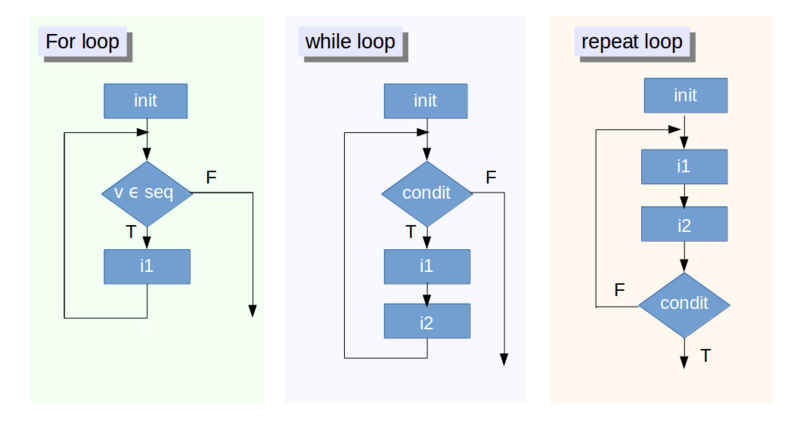
\includegraphics{./tex2pdf.956/645ce298d09f8b6a04c4b9ecab4d619cedfffc6d.png}

\end{frame}

\begin{frame}[fragile]{Beispiele für
\href{https://www.r-bloggers.com/how-to-write-the-first-for-loop-in-r/}{Schleifen}}

\begin{block}{Beispiel Jahreszahlen plotten}

\begin{Shaded}
\begin{Highlighting}[]
\NormalTok{for (year in }\KeywordTok{c}\NormalTok{(}\DecValTok{2010}\NormalTok{,}\DecValTok{2011}\NormalTok{,}\DecValTok{2012}\NormalTok{,}\DecValTok{2013}\NormalTok{,}\DecValTok{2014}\NormalTok{,}\DecValTok{2015}\NormalTok{))\{}
  \KeywordTok{print}\NormalTok{(}\KeywordTok{paste}\NormalTok{(}\StringTok{"The year is"}\NormalTok{, year))}
\NormalTok{\}}
\end{Highlighting}
\end{Shaded}

\end{block}

\begin{block}{Beispiel: Ergebnisse der Schleife in Container speichern}

\begin{Shaded}
\begin{Highlighting}[]
\NormalTok{erg <-}\StringTok{ }\KeywordTok{vector}\NormalTok{()}

\NormalTok{for (i in }\DecValTok{1}\NormalTok{:}\KeywordTok{ncol}\NormalTok{(dat))\{}
  \NormalTok{erg[i] <-}\StringTok{ }\KeywordTok{mean}\NormalTok{(}\KeywordTok{runif}\NormalTok{(}\DecValTok{100}\NormalTok{))}
\NormalTok{\}}
\end{Highlighting}
\end{Shaded}

\end{block}

\end{frame}

\begin{frame}[fragile]{\href{http://faculty.nps.edu/sebuttre/home/R/missings.html}{Fehlende
Werte ausschließen}}

\begin{itemize}
\tightlist
\item
  Mathe-Funktionen haben in der Regel einen Weg, um fehlende Werte in
  ihren Berechnungen auszuschließen.
\item
  \texttt{mean(),\ median(),\ colSums(),\ var(),\ sd(),\ min()} und
  `max() all take the na.rm argument.
\end{itemize}

\end{frame}

\begin{frame}[fragile]{Fehlende Werte umkodieren}

\begin{Shaded}
\begin{Highlighting}[]
\NormalTok{Daten$bazq020a[Daten$bazq020a==-}\DecValTok{99}\NormalTok{] <-}\StringTok{ }\OtherTok{NA}
\end{Highlighting}
\end{Shaded}

\begin{itemize}
\item
  \href{http://www.statmethods.net/input/missingdata.html}{Quick-R zu
  fehlenden Werten}
\item
  \href{http://uc-r.github.io/na_recode}{Fehlende Werte rekodieren}
\end{itemize}

\end{frame}

\begin{frame}[fragile]{Mit Strings arbeiten}

\begin{Shaded}
\begin{Highlighting}[]
\KeywordTok{gsub}\NormalTok{(}\StringTok{"l"}\NormalTok{,}\StringTok{"L"}\NormalTok{,}\StringTok{"Hallo Welt"}\NormalTok{)}
\end{Highlighting}
\end{Shaded}

\begin{verbatim}
## [1] "HaLLo WeLt"
\end{verbatim}

\begin{itemize}
\tightlist
\item
  \href{https://github.com/statsmaths/useR2017_nlp}{Natural Language
  Processing - Tutorial auf der UseR 2017}
\end{itemize}

\end{frame}

\begin{frame}[fragile]{Weitere Links}

\begin{itemize}
\item
  \href{https://cran.r-project.org/web/packages/googleVis/vignettes/googleVis_examples.html}{Das
  \texttt{googleVis} Paket für einen besseren Überblick}
\item
  \href{https://cran.r-project.org/web/packages/tidyr/vignettes/tidy-data.html}{Tidy
  data} - das Paket \texttt{tidyr}
\item
  \href{http://tidyverse.org/}{Die \texttt{tidyverse} Sammlung}
\item
  \href{https://www.rstudio.com/resources/webinars/data-wrangling-with-r-and-rstudio/}{Data
  wrangling with R and RStudio}
\end{itemize}

\end{frame}

\begin{frame}{Datenexport}

\end{frame}

\begin{frame}[fragile]{Die Exportformate von R}

\begin{itemize}
\tightlist
\item
  In R werden offene Dateiformate bevorzugt
\item
  Genauso wie \texttt{read.X()} Funktionen stehen viele
  \texttt{write.X()} Funktionen zur Verfügung
\item
  Das eigene Format von R sind sog. Workspaces (\texttt{.RData})
\end{itemize}

\end{frame}

\begin{frame}[fragile]{Beispieldatensatz erzeugen}

\begin{Shaded}
\begin{Highlighting}[]
\NormalTok{A <-}\StringTok{ }\KeywordTok{c}\NormalTok{(}\DecValTok{1}\NormalTok{,}\DecValTok{2}\NormalTok{,}\DecValTok{3}\NormalTok{,}\DecValTok{4}\NormalTok{)}
\NormalTok{B <-}\StringTok{ }\KeywordTok{c}\NormalTok{(}\StringTok{"A"}\NormalTok{,}\StringTok{"B"}\NormalTok{,}\StringTok{"C"}\NormalTok{,}\StringTok{"D"}\NormalTok{)}

\NormalTok{mydata <-}\StringTok{ }\KeywordTok{data.frame}\NormalTok{(A,B)}
\end{Highlighting}
\end{Shaded}

\begin{longtable}[]{@{}rl@{}}
\toprule
A & B\tabularnewline
\midrule
\endhead
1 & A\tabularnewline
2 & B\tabularnewline
3 & C\tabularnewline
4 & D\tabularnewline
\bottomrule
\end{longtable}

\end{frame}

\begin{frame}[fragile]{Überblick Daten Import/Export}

\begin{itemize}
\tightlist
\item
  wenn mit R weitergearbeitet wird, eignet sich das \texttt{.RData}
  Format am Besten:
\end{itemize}

\begin{Shaded}
\begin{Highlighting}[]
\KeywordTok{save}\NormalTok{(mydata, }\DataTypeTok{file=}\StringTok{"mydata.RData"}\NormalTok{)}
\end{Highlighting}
\end{Shaded}

\begin{itemize}
\tightlist
\item
  Der Datensatz kann dann mit \texttt{load} wieder eingelesen werden
\end{itemize}

\begin{Shaded}
\begin{Highlighting}[]
\KeywordTok{load}\NormalTok{(}\StringTok{"mydata.RData"}\NormalTok{)}
\end{Highlighting}
\end{Shaded}

\end{frame}

\begin{frame}[fragile]{Daten in \texttt{.csv} Format abspeichern}

\begin{Shaded}
\begin{Highlighting}[]
\KeywordTok{write.csv}\NormalTok{(mydata,}\DataTypeTok{file=}\StringTok{"mydata.csv"}\NormalTok{) }
\end{Highlighting}
\end{Shaded}

\begin{itemize}
\tightlist
\item
  Wenn mit Deutschem Excel weitergearbeitet werden soll, eignet sich
  \texttt{write.csv2} besser
\end{itemize}

\begin{Shaded}
\begin{Highlighting}[]
\KeywordTok{write.csv2}\NormalTok{(mydata,}\DataTypeTok{file=}\StringTok{"mydata.csv"}\NormalTok{) }
\end{Highlighting}
\end{Shaded}

\begin{itemize}
\tightlist
\item
  Sonst sieht das Ergebnis so aus:
\end{itemize}

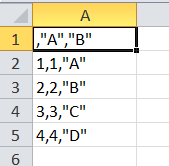
\includegraphics{./tex2pdf.956/18fa31a6671691665971d435cb85f1252e5f17a0.png}

\end{frame}

\begin{frame}[fragile]{\href{http://www.sthda.com/english/wiki/r-xlsx-package-a-quick-start-guide-to-manipulate-excel-files-in-r\#read-an-excel-file}{Das
Paket \texttt{xlsx}}}

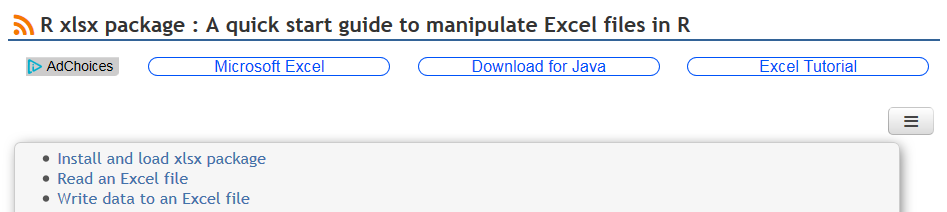
\includegraphics{./tex2pdf.956/f8e4fe7da5e630832ec7e1566b80a8d388b852cb.png}

\begin{Shaded}
\begin{Highlighting}[]
\KeywordTok{library}\NormalTok{(xlsx)}
\KeywordTok{write.xlsx}\NormalTok{(mydata,}\DataTypeTok{file=}\StringTok{"mydata.xlsx"}\NormalTok{) }
\end{Highlighting}
\end{Shaded}

\end{frame}

\begin{frame}[fragile]{\href{https://www.r-bloggers.com/readingwriting-stata-dta-files-with-foreign/}{Das
Paket \texttt{foreign}}}


\includegraphics{./tex2pdf.956/cacdeac9e2a94bf873762c46b11f6576b5bf7fd2.png}

\begin{itemize}
\tightlist
\item
  Funktionen im Paket \texttt{foreign}
\end{itemize}

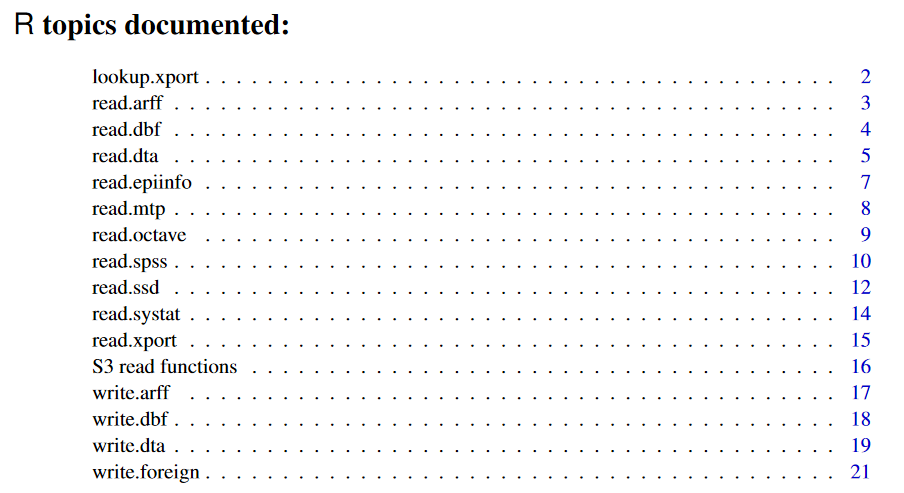
\includegraphics{./tex2pdf.956/127b4a21c6edd4bea1001fe04e85f4f5a06b9ec8.png}

\end{frame}

\begin{frame}[fragile]{Daten in stata Format abspeichern}

\begin{Shaded}
\begin{Highlighting}[]
\KeywordTok{library}\NormalTok{(foreign)}
\KeywordTok{write.dta}\NormalTok{(mydata,}\DataTypeTok{file=}\StringTok{"data/mydata.dta"}\NormalTok{) }
\end{Highlighting}
\end{Shaded}

\end{frame}

\begin{frame}[fragile]{Das Paket \texttt{rio}}

\begin{Shaded}
\begin{Highlighting}[]
\KeywordTok{install.packages}\NormalTok{(}\StringTok{"rio"}\NormalTok{)}
\end{Highlighting}
\end{Shaded}

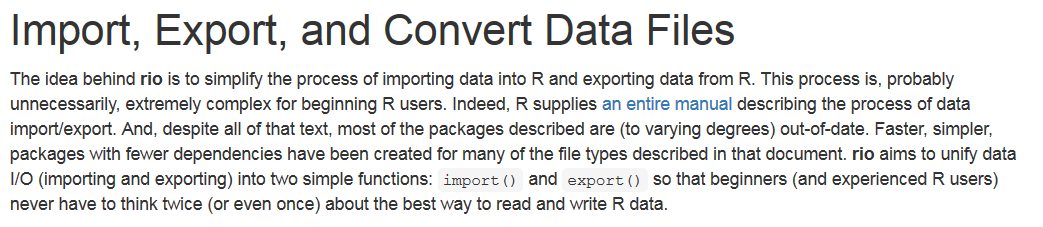
\includegraphics{./tex2pdf.956/ac65f614039096ed31ca6b9fb206c3472a6ba9cb.png}

\end{frame}

\begin{frame}[fragile]{\href{https://cran.r-project.org/web/packages/rio/vignettes/rio.html}{Daten
als .sav abspeichern (SPSS)}}

\begin{Shaded}
\begin{Highlighting}[]
\KeywordTok{library}\NormalTok{(}\StringTok{"rio"}\NormalTok{)}
\CommentTok{# create file to convert}

\KeywordTok{export}\NormalTok{(mtcars, }\StringTok{"data/mtcars.sav"}\NormalTok{)}
\end{Highlighting}
\end{Shaded}

\end{frame}

\begin{frame}[fragile]{Dateiformate konvertieren}

\begin{Shaded}
\begin{Highlighting}[]
\KeywordTok{export}\NormalTok{(mtcars, }\StringTok{"data/mtcars.dta"}\NormalTok{)}

\CommentTok{# convert Stata to SPSS}
\KeywordTok{convert}\NormalTok{(}\StringTok{"data/mtcars.dta"}\NormalTok{, }\StringTok{"data/mtcars.sav"}\NormalTok{)}
\end{Highlighting}
\end{Shaded}

\end{frame}

\begin{frame}{Links Export}

\begin{itemize}
\item
  \href{http://www.statmethods.net/input/exportingdata.html}{Quick R}
  für das Exportieren von Daten:
\item
  Hilfe zum Export auf dem
  \href{http://cran.r-project.org/doc/manuals/r-release/R-data.pdf}{cran
  Server}
\item
  \href{https://www.stat.ubc.ca/~jenny/STAT545A/block05_getNumbersOut.html}{Daten
  aus R heraus bekommen}
\end{itemize}

\end{frame}

\begin{frame}[fragile]{Aufgabe - OECD Datensatz}

\begin{itemize}
\tightlist
\item
  Laden Sie den
  \href{https://raw.githubusercontent.com/Japhilko/IntroR/master/2015/data/oecd.csv}{oecd-Datensatz}
  herunter und lesen Sie ihn mit folgender Funktion ein:
\end{itemize}

\url{https://raw.githubusercontent.com/Japhilko/IntroR/master/2015/data/oecd.csv}

\begin{Shaded}
\begin{Highlighting}[]
\NormalTok{link <-}\StringTok{ "https://raw.githubusercontent.com/Japhilko/IntroR/master/2015/data/oecd.csv"}
\NormalTok{data <-}\StringTok{ }\KeywordTok{read.csv}\NormalTok{(link)}
\end{Highlighting}
\end{Shaded}

\begin{itemize}
\item
  Überprüfen Sie die Dimensioenn der OECD-Daten.
\item
  Berechnen Sie die Mittelwerte und Varianzen der einzelnen Variablen
  mit einem geeigneten apply Befehl.
\item
  In welchem Land waren die meisten Jugendlichen mindestens zweimal
  betrunken (Spalte Alkohol)? Wie hoch ist der maximale Prozentsatz?
\item
  In welchem Land ist die Sterblichkeit am geringsten? Wie hoch ist sie
  in diesem Land?
\item
  Erstellen Sie einen neuen Datensatz, der aufsteigend nach dem
  Einkommen geordnet ist. Speichern Sie diesen in einer neuen .csv Datei
\end{itemize}

\end{frame}

\begin{frame}{Basisgrafiken}

\end{frame}

\begin{frame}{Ein Plot sagt mehr als 1000 Worte}

\begin{itemize}
\tightlist
\item
  Grafisch gestützte Datenanalyse ist toll
\item
  Gute Plots können zu einem besseren Verständnis beitragen
\item
  Einen Plot zu generieren geht schnell
\item
  Einen guten Plot zu machen kann sehr lange dauern
\item
  Mit R Plots zu generieren macht Spaß
\item
  Mit R erstellte Plots haben hohe Qualität
\item
  Fast jeder Plottyp wird von R unterstützt
\item
  R kennt eine große Menge an Exportformaten für Grafiken
\end{itemize}

\end{frame}

\begin{frame}{Plot ist nicht gleich Plot}

\begin{itemize}
\tightlist
\item
  Bereits das base Package bringt eine große Menge von Plot Funktionen
  mit
\item
  Das lattice Packet erweitert dessen Funktionalität
\item
  Eine weit über diese Einführung hinausgehende Übersicht findet sich in
  Murrell, P (2006): R Graphics.
\end{itemize}

\end{frame}

\begin{frame}{Task View zu Thema
\href{https://cran.r-project.org/web/views/Graphics.html}{Graphiken}}

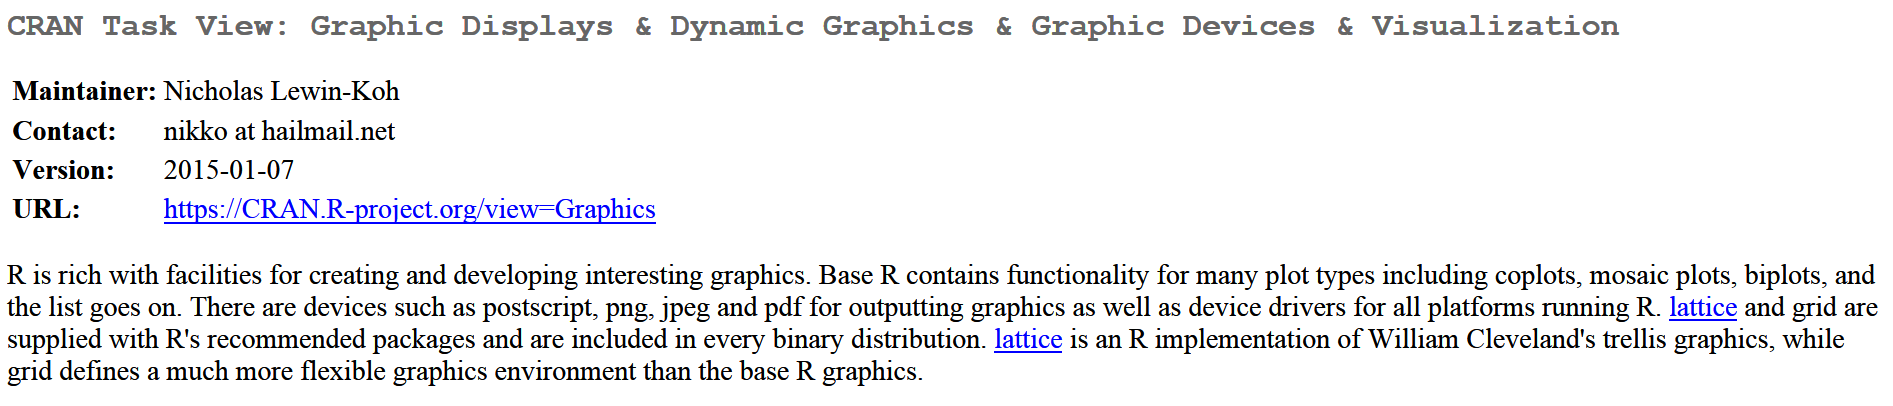
\includegraphics{./tex2pdf.956/5e4adb82cb6141da7bafecd33dfdc7d0e44f95dc.png}

\end{frame}

\begin{frame}[fragile]{Datensatz}

\begin{Shaded}
\begin{Highlighting}[]
\KeywordTok{library}\NormalTok{(mlmRev)}
\KeywordTok{data}\NormalTok{(Chem97)}
\end{Highlighting}
\end{Shaded}

\begin{itemize}
\tightlist
\item
  {[}lea{]} Local Education Authority - a factor
\item
  {[}school{]} School identifier - a factor
\item
  {[}student{]} Student identifier - a factor
\item
  {[}score{]} Point score on A-level Chemistry in 1997
\item
  {[}gender{]} Student's gender
\item
  {[}age{]} Age in month, centred at 222 months or 18.5 years
\item
  {[}gcsescore{]} Average GCSE score of individual.
\item
  {[}gcsecnt{]} Average GCSE score of individual, centered at mean.
\end{itemize}

\end{frame}

\begin{frame}[fragile]{Histogramm - Die Funktion hist()}

Wir erstellen ein Histogramm der Variable gcsescore (Hilfe mit
\texttt{?hist}):

\begin{Shaded}
\begin{Highlighting}[]
\KeywordTok{hist}\NormalTok{(Chem97$gcsescore)}
\end{Highlighting}
\end{Shaded}

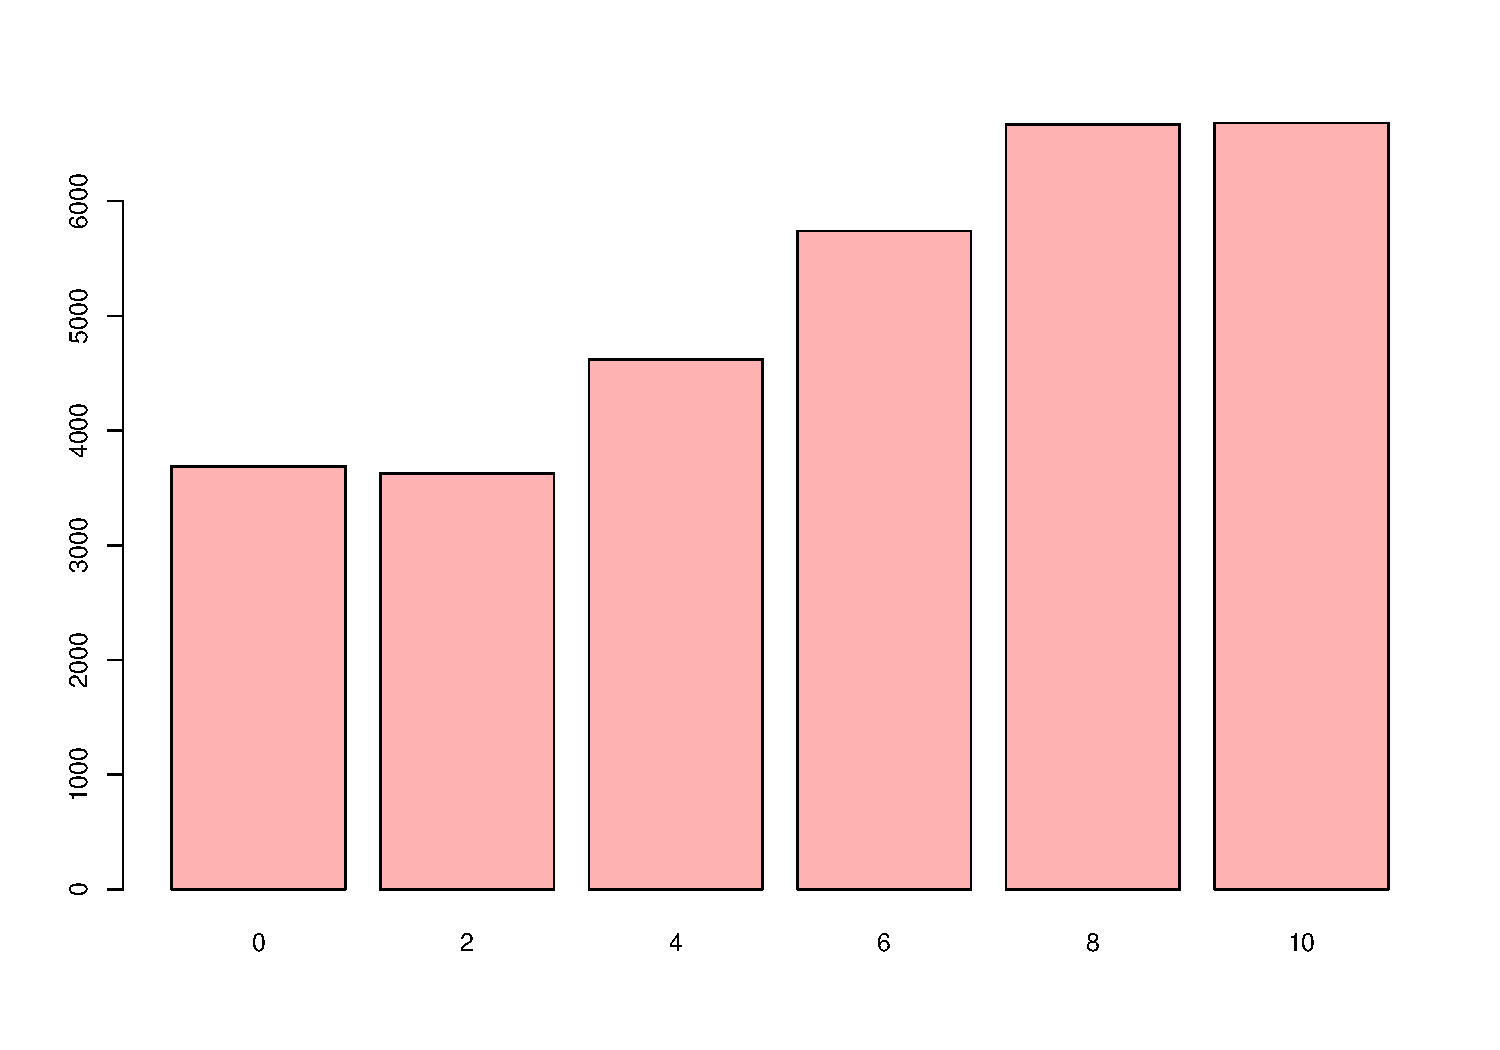
\includegraphics{R_intern_files/figure-beamer/unnamed-chunk-149-1.pdf}

\end{frame}

\begin{frame}{Graphik speichern}

\begin{itemize}
\tightlist
\item
  Mit dem button Export in Rstudio kann man die Grafik speichern.
\end{itemize}

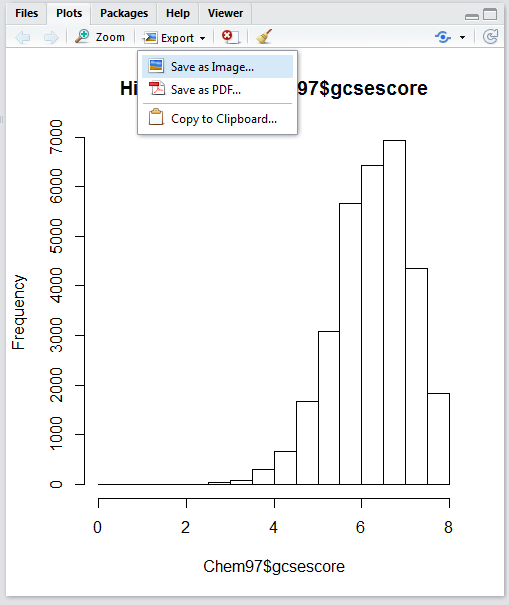
\includegraphics{./tex2pdf.956/c841157f024cc7a3d01009eeb5c876036fad5d81.png}

\end{frame}

\begin{frame}[fragile]{Befehl um Graphik zu speichern}

\begin{itemize}
\tightlist
\item
  Alternativ auch bspw. mit den Befehlen \texttt{png}, \texttt{pdf} oder
  \texttt{jpeg}
\end{itemize}

\begin{Shaded}
\begin{Highlighting}[]
\KeywordTok{png}\NormalTok{(}\StringTok{"Histogramm.png"}\NormalTok{)}
\KeywordTok{hist}\NormalTok{(Chem97$gcsescore)}
\KeywordTok{dev.off}\NormalTok{()}
\end{Highlighting}
\end{Shaded}

\end{frame}

\begin{frame}[fragile]{Histogramme}

\begin{itemize}
\tightlist
\item
  Die Funktion \texttt{hist()} plottet ein Histogramm der Daten
\item
  Der Funktion muss mindestens ein Beobachtungsvektor übergeben werden
\item
  \texttt{hist()} hat noch sehr viel mehr Argumente, die alle
  (sinnvolle) default values haben
\end{itemize}

\begin{longtable}[]{@{}lll@{}}
\toprule
Argument & Bedeutung & Beispiel\tabularnewline
\midrule
\endhead
main & Überschrift & main=``Hallo Welt''\tabularnewline
xlab & x-Achsenbeschriftung & xlab=``x-Werte''\tabularnewline
ylab & y-Achsenbeschriftung & ylab=``y-Werte''\tabularnewline
col & Farbe & col=``blue''\tabularnewline
\bottomrule
\end{longtable}

\end{frame}

\begin{frame}[fragile]{Histogramm}

\begin{Shaded}
\begin{Highlighting}[]
\KeywordTok{hist}\NormalTok{(Chem97$gcsescore,}\DataTypeTok{col=}\StringTok{"blue"}\NormalTok{,}
     \DataTypeTok{main=}\StringTok{"Hallo Welt"}\NormalTok{,}\DataTypeTok{ylab=}\StringTok{"y-Werte"}\NormalTok{, }\DataTypeTok{xlab=}\StringTok{"x-Werte"}\NormalTok{)}
\end{Highlighting}
\end{Shaded}

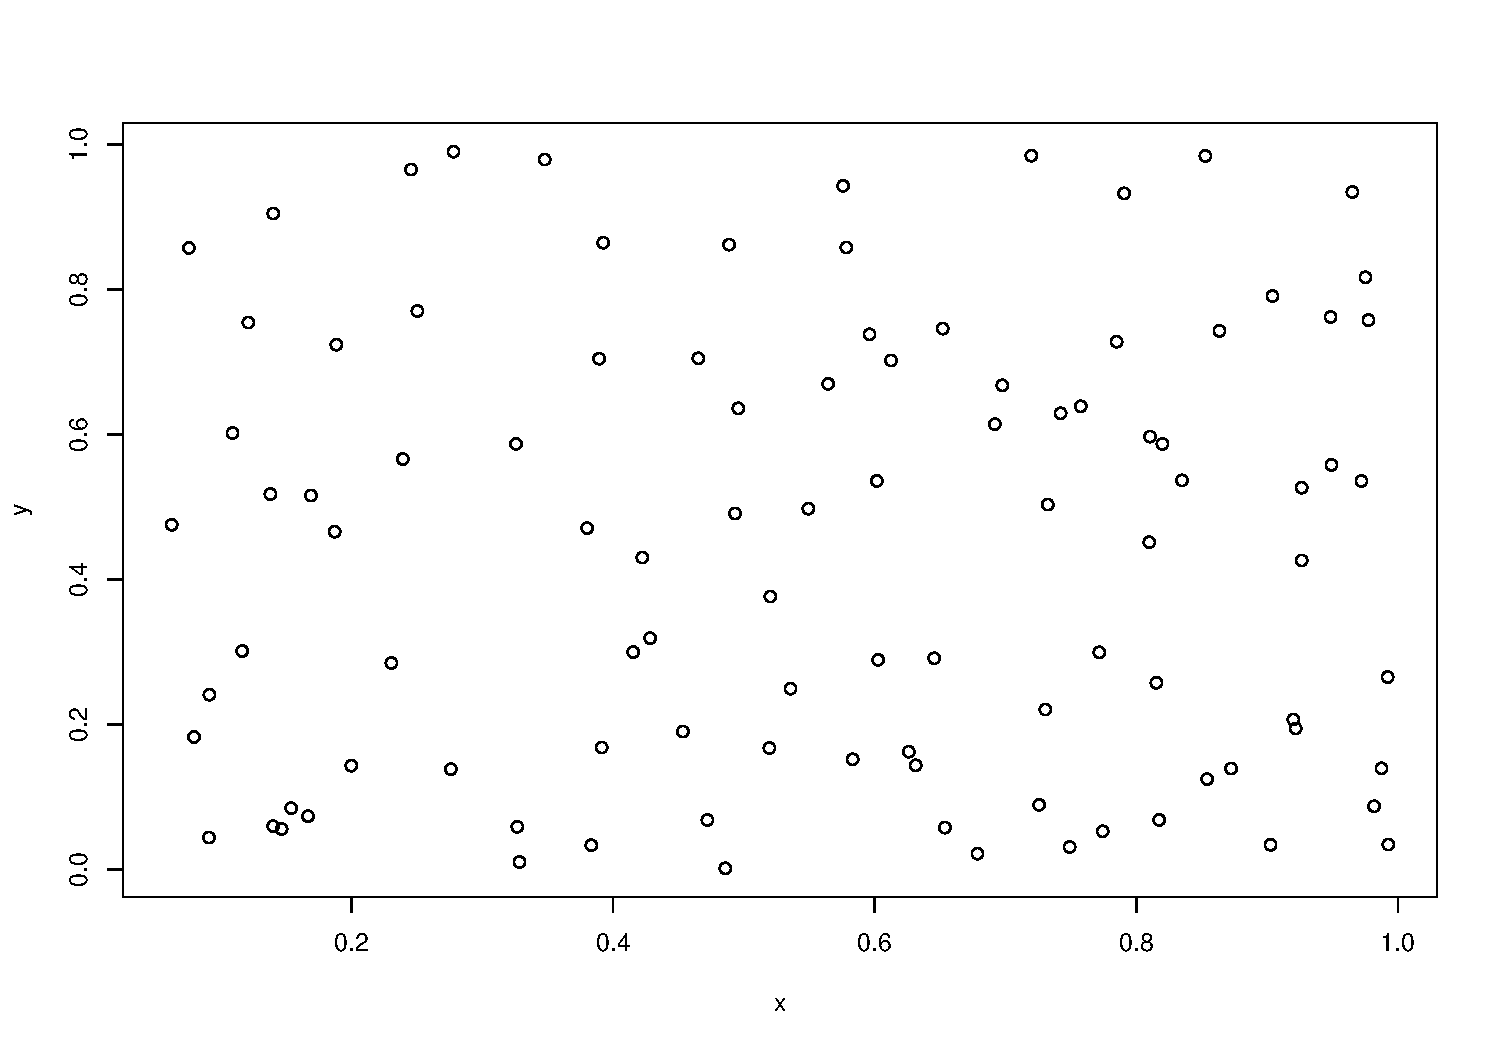
\includegraphics{R_intern_files/figure-beamer/unnamed-chunk-151-1.pdf}

Weitere Argumente:

\begin{Shaded}
\begin{Highlighting}[]
\NormalTok{?plot}
\CommentTok{# oder}
\NormalTok{?par}
\end{Highlighting}
\end{Shaded}

\end{frame}

\begin{frame}[fragile]{Barplot}

\begin{itemize}
\tightlist
\item
  Die Funktion \texttt{barplot()} erzeugt aus einer Häufigkeitstabelle
  einen Barplot
\item
  Ist das übergebene Tabellen-Objekt zweidimensional wird ein bedingter
  Barplot erstellt
\end{itemize}

\begin{Shaded}
\begin{Highlighting}[]
\NormalTok{tabScore <-}\StringTok{ }\KeywordTok{table}\NormalTok{(Chem97$score)}
\end{Highlighting}
\end{Shaded}

\begin{Shaded}
\begin{Highlighting}[]
\KeywordTok{barplot}\NormalTok{(tabScore)}
\end{Highlighting}
\end{Shaded}

\end{frame}

\begin{frame}[fragile]{Barplots und barcharts}

\begin{Shaded}
\begin{Highlighting}[]
\KeywordTok{barplot}\NormalTok{(tabScore)}
\end{Highlighting}
\end{Shaded}

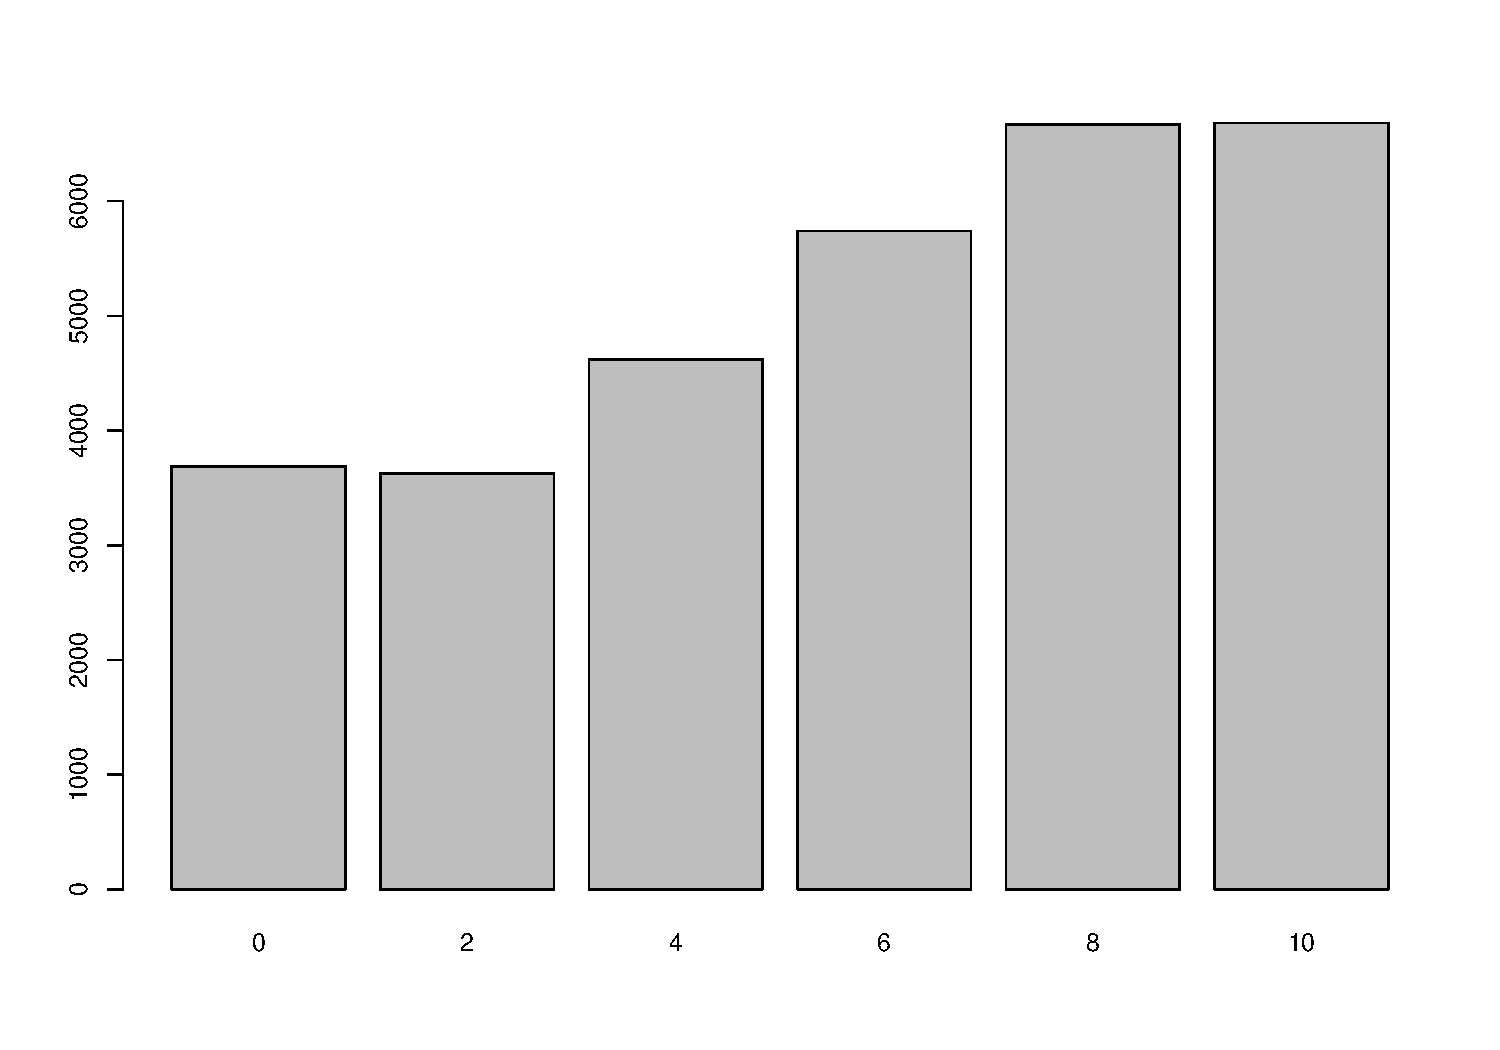
\includegraphics{R_intern_files/figure-beamer/unnamed-chunk-155-1.pdf}

\end{frame}

\begin{frame}[fragile]{Mehr Farben:}

\begin{Shaded}
\begin{Highlighting}[]
\KeywordTok{barplot}\NormalTok{(tabScore,}\DataTypeTok{col=}\KeywordTok{rgb}\NormalTok{(}\DecValTok{0}\NormalTok{,}\DecValTok{0}\NormalTok{,}\DecValTok{1}\NormalTok{))}
\end{Highlighting}
\end{Shaded}

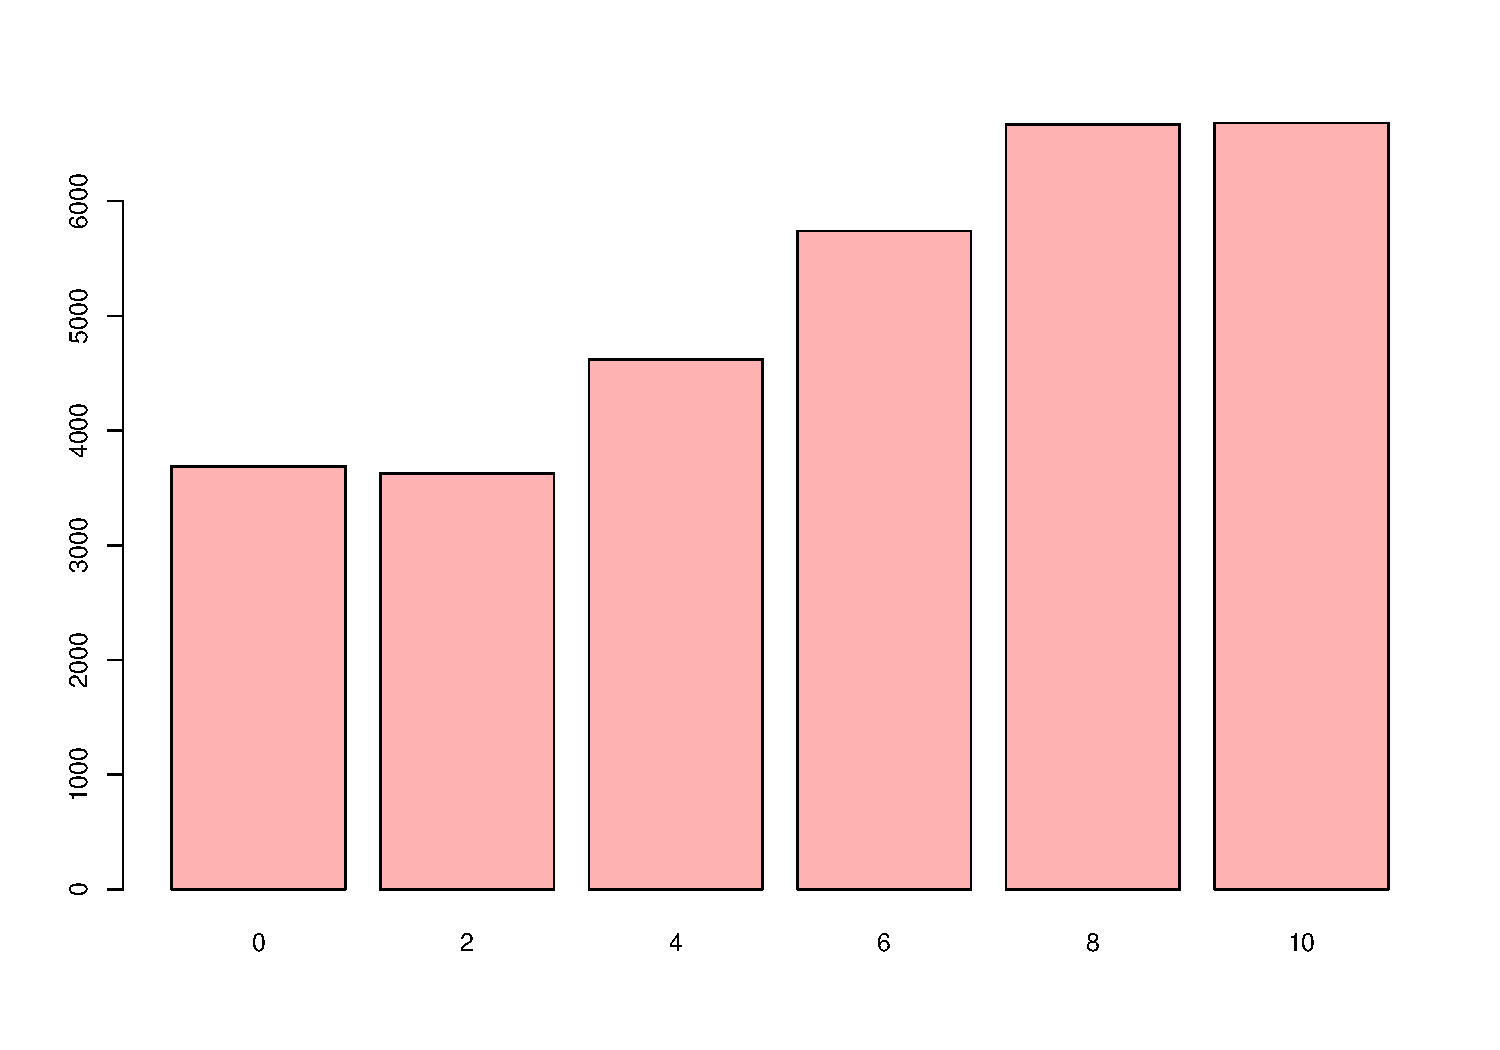
\includegraphics{R_intern_files/figure-beamer/unnamed-chunk-156-1.pdf}

\end{frame}

\begin{frame}[fragile]{Grüne Farbe}

\begin{Shaded}
\begin{Highlighting}[]
\KeywordTok{barplot}\NormalTok{(tabScore,}\DataTypeTok{col=}\KeywordTok{rgb}\NormalTok{(}\DecValTok{0}\NormalTok{,}\DecValTok{1}\NormalTok{,}\DecValTok{0}\NormalTok{))}
\end{Highlighting}
\end{Shaded}

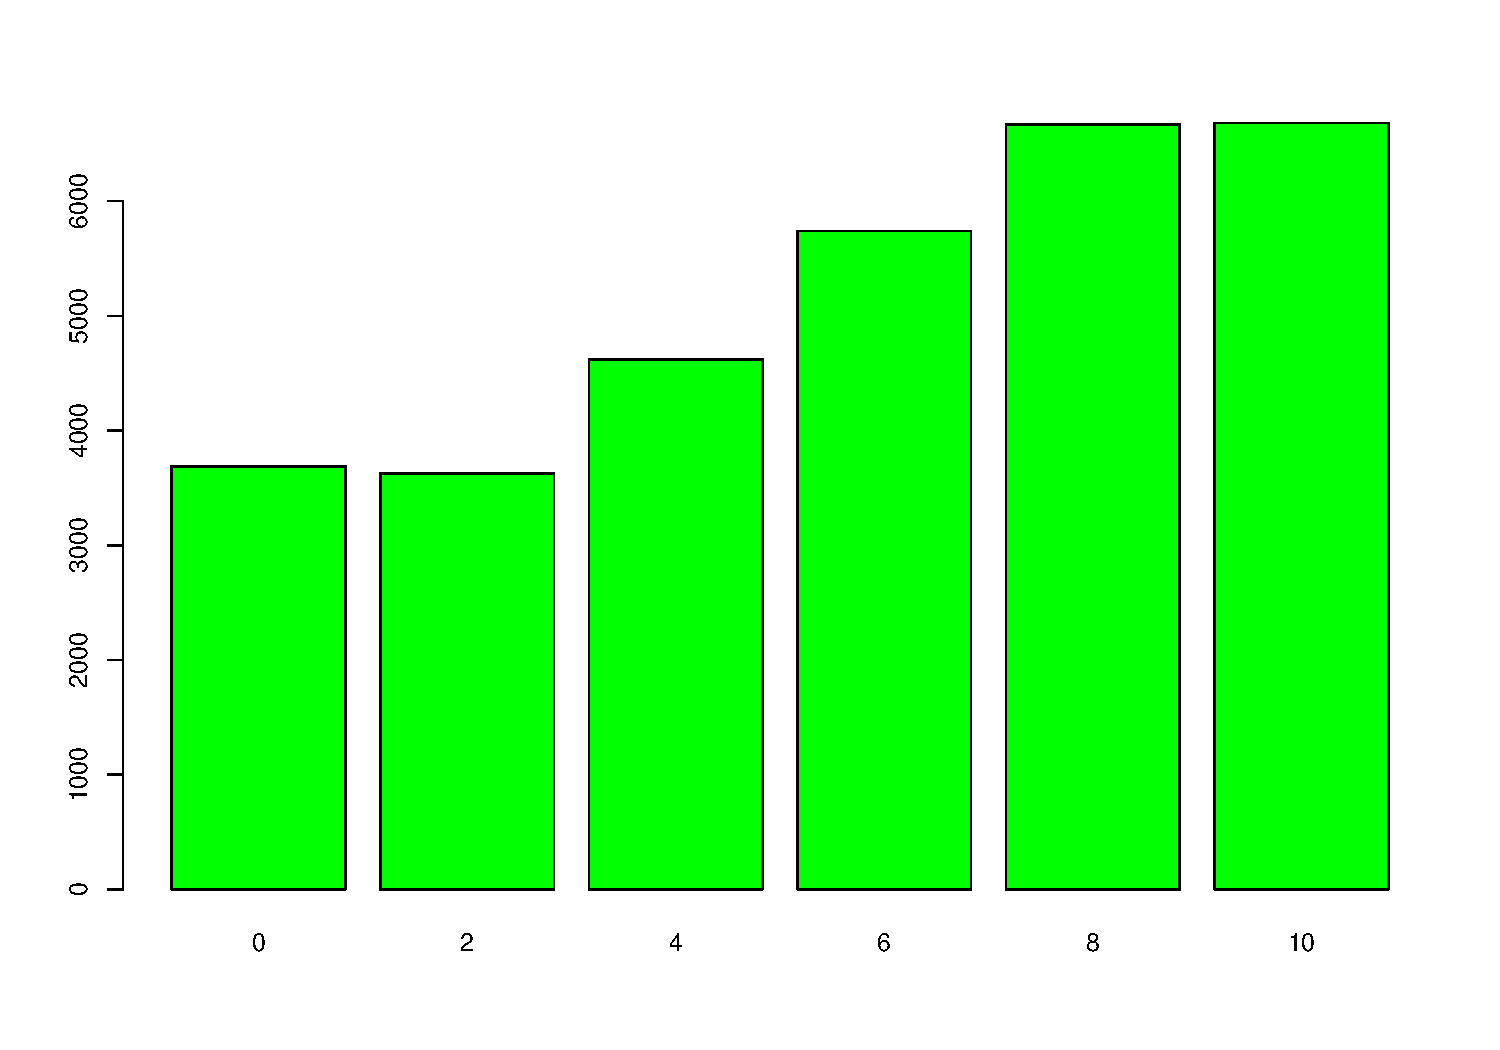
\includegraphics{R_intern_files/figure-beamer/unnamed-chunk-157-1.pdf}

\end{frame}

\begin{frame}[fragile]{Rote Farbe}

\begin{Shaded}
\begin{Highlighting}[]
\KeywordTok{barplot}\NormalTok{(tabScore,}\DataTypeTok{col=}\KeywordTok{rgb}\NormalTok{(}\DecValTok{1}\NormalTok{,}\DecValTok{0}\NormalTok{,}\DecValTok{0}\NormalTok{))}
\end{Highlighting}
\end{Shaded}

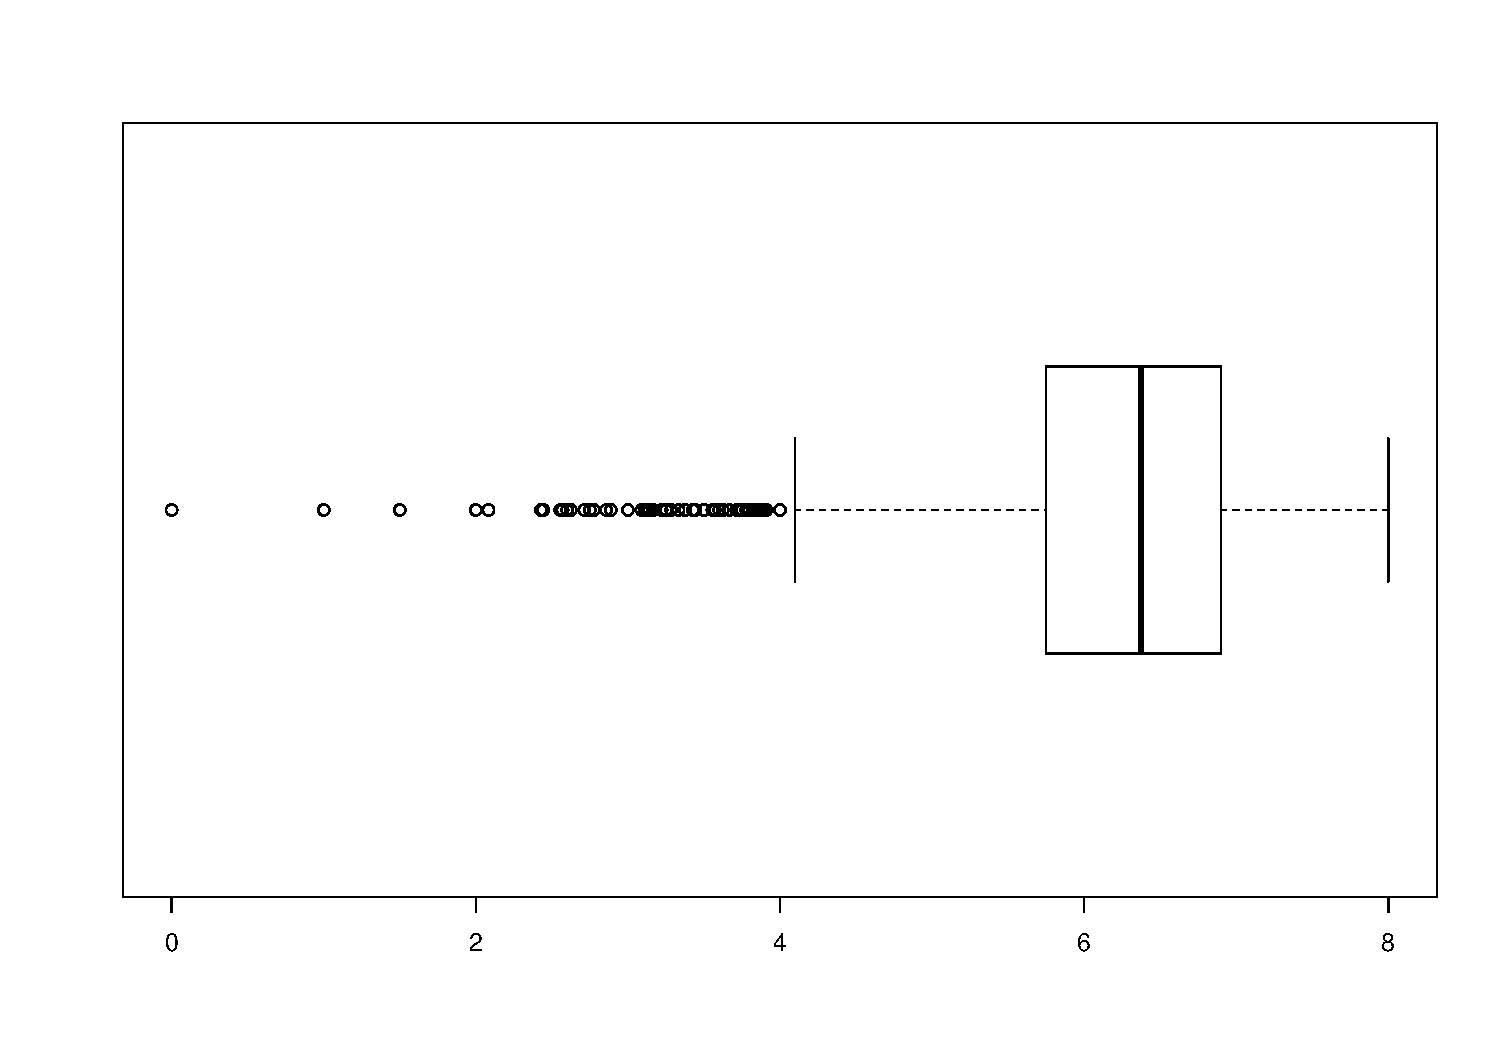
\includegraphics{R_intern_files/figure-beamer/unnamed-chunk-158-1.pdf}

\end{frame}

\begin{frame}[fragile]{Transparent}

\begin{Shaded}
\begin{Highlighting}[]
\KeywordTok{barplot}\NormalTok{(tabScore,}\DataTypeTok{col=}\KeywordTok{rgb}\NormalTok{(}\DecValTok{1}\NormalTok{,}\DecValTok{0}\NormalTok{,}\DecValTok{0}\NormalTok{,.}\DecValTok{3}\NormalTok{))}
\end{Highlighting}
\end{Shaded}

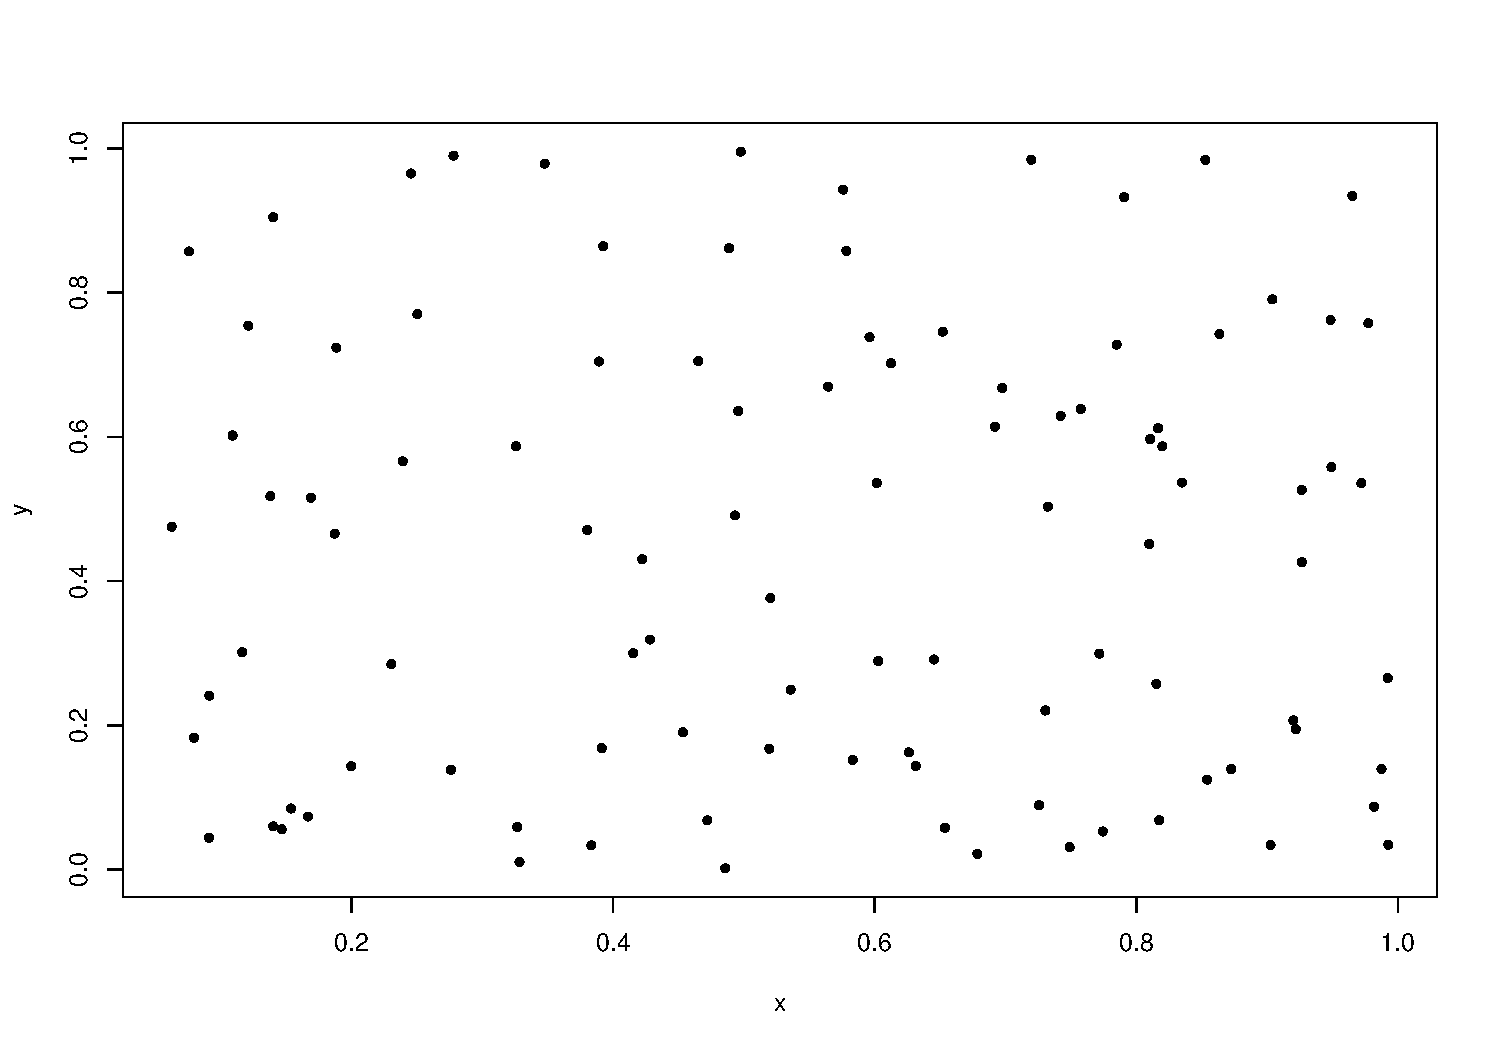
\includegraphics{R_intern_files/figure-beamer/unnamed-chunk-159-1.pdf}

\end{frame}

\begin{frame}{Scatterplots}

\begin{itemize}
\tightlist
\item
  Ein einfacher two-way Scatterplot kann mit der Funktion plot()
  erstellt werden
\item
  plot() muss mindestens ein x und ein y Beobachtungsvektor übergeben
  werden
\item
  Um die Farbe der Plot-Symbole anzupassen gibt es die Option col (Farbe
  als character oder numerisch)
\item
  Die Plot-Symbole selbst können mit pch (plotting character) angepasst
  werden (character oder numerisch)
\item
  Die Achenbeschriftungen (labels) werden mit xlab und ylab definiert
\end{itemize}

\end{frame}

\begin{frame}[fragile]{Beispieldaten für Scatterplot}

\begin{Shaded}
\begin{Highlighting}[]
\NormalTok{x <-}\StringTok{ }\KeywordTok{runif}\NormalTok{(}\DecValTok{100}\NormalTok{)}
\KeywordTok{head}\NormalTok{(x)}
\end{Highlighting}
\end{Shaded}

\begin{verbatim}
## [1] 0.5693192 0.4434360 0.5771024 0.8077336 0.1885673 0.7494796
\end{verbatim}

\begin{Shaded}
\begin{Highlighting}[]
\NormalTok{y <-}\StringTok{ }\KeywordTok{runif}\NormalTok{(}\DecValTok{100}\NormalTok{)}
\KeywordTok{head}\NormalTok{(y)}
\end{Highlighting}
\end{Shaded}

\begin{verbatim}
## [1] 0.83281135 0.17390341 0.44462134 0.20738954 0.44803019 0.01901425
\end{verbatim}

\end{frame}

\begin{frame}[fragile]{Einfacher Scatterplot}

\begin{Shaded}
\begin{Highlighting}[]
\KeywordTok{plot}\NormalTok{(x,y)}
\end{Highlighting}
\end{Shaded}

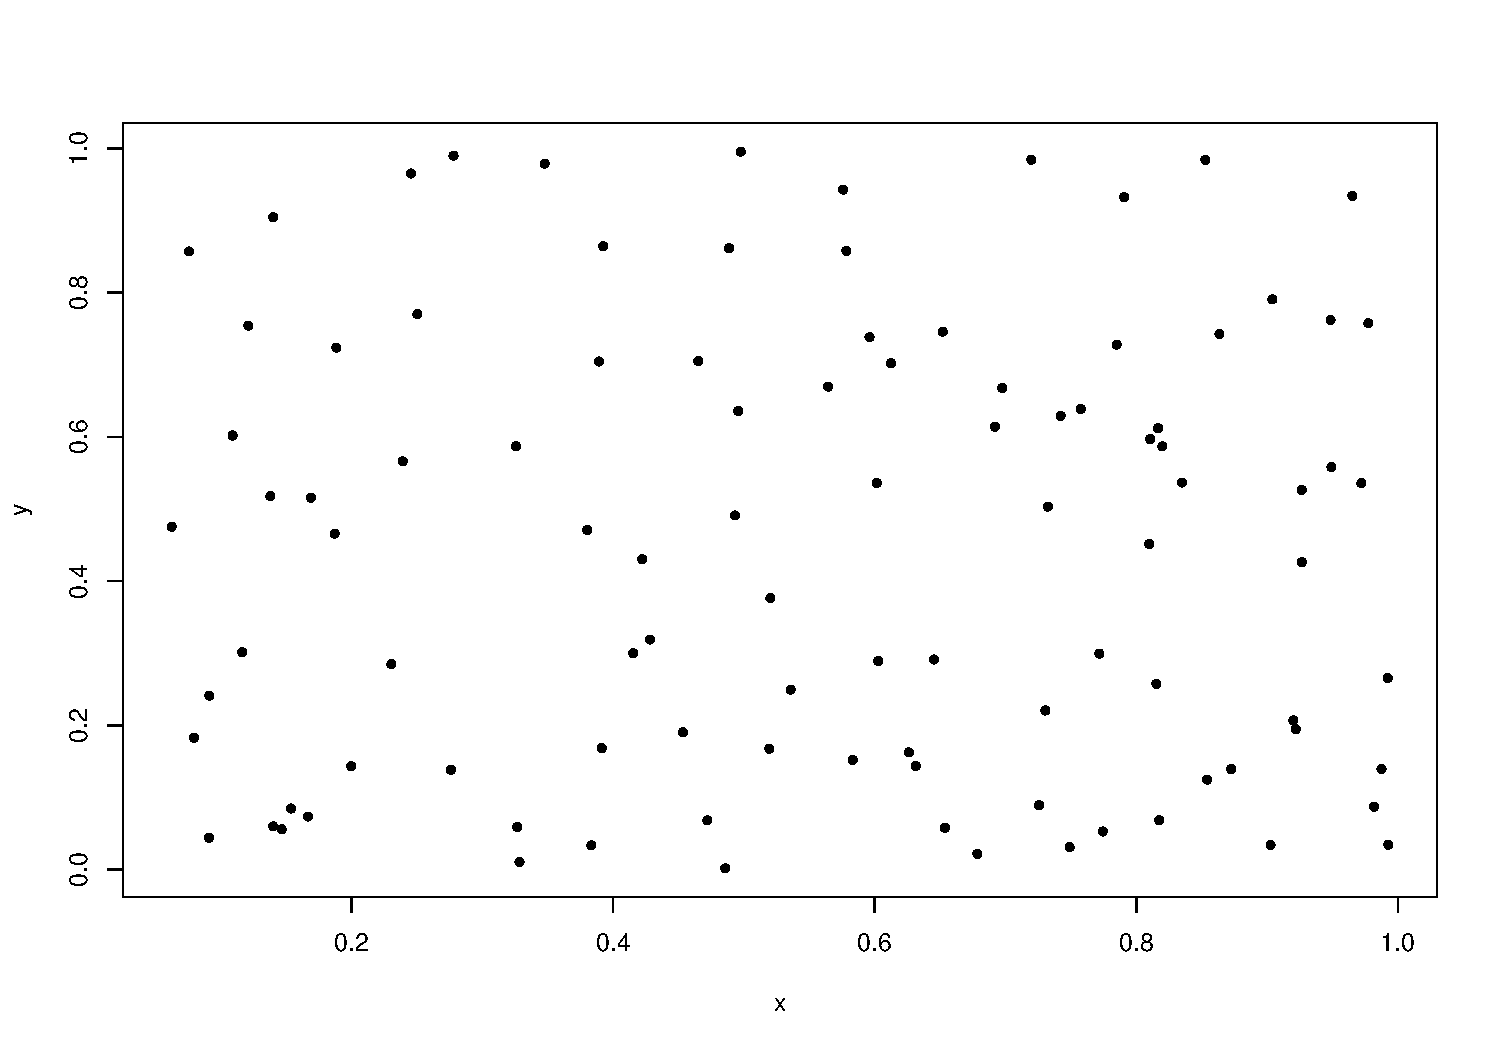
\includegraphics{R_intern_files/figure-beamer/unnamed-chunk-161-1.pdf}

\end{frame}

\begin{frame}[fragile]{Einfacher Scatterplot II}

\begin{Shaded}
\begin{Highlighting}[]
\KeywordTok{plot}\NormalTok{(x,y,}\DataTypeTok{pch=}\DecValTok{20}\NormalTok{)}
\end{Highlighting}
\end{Shaded}

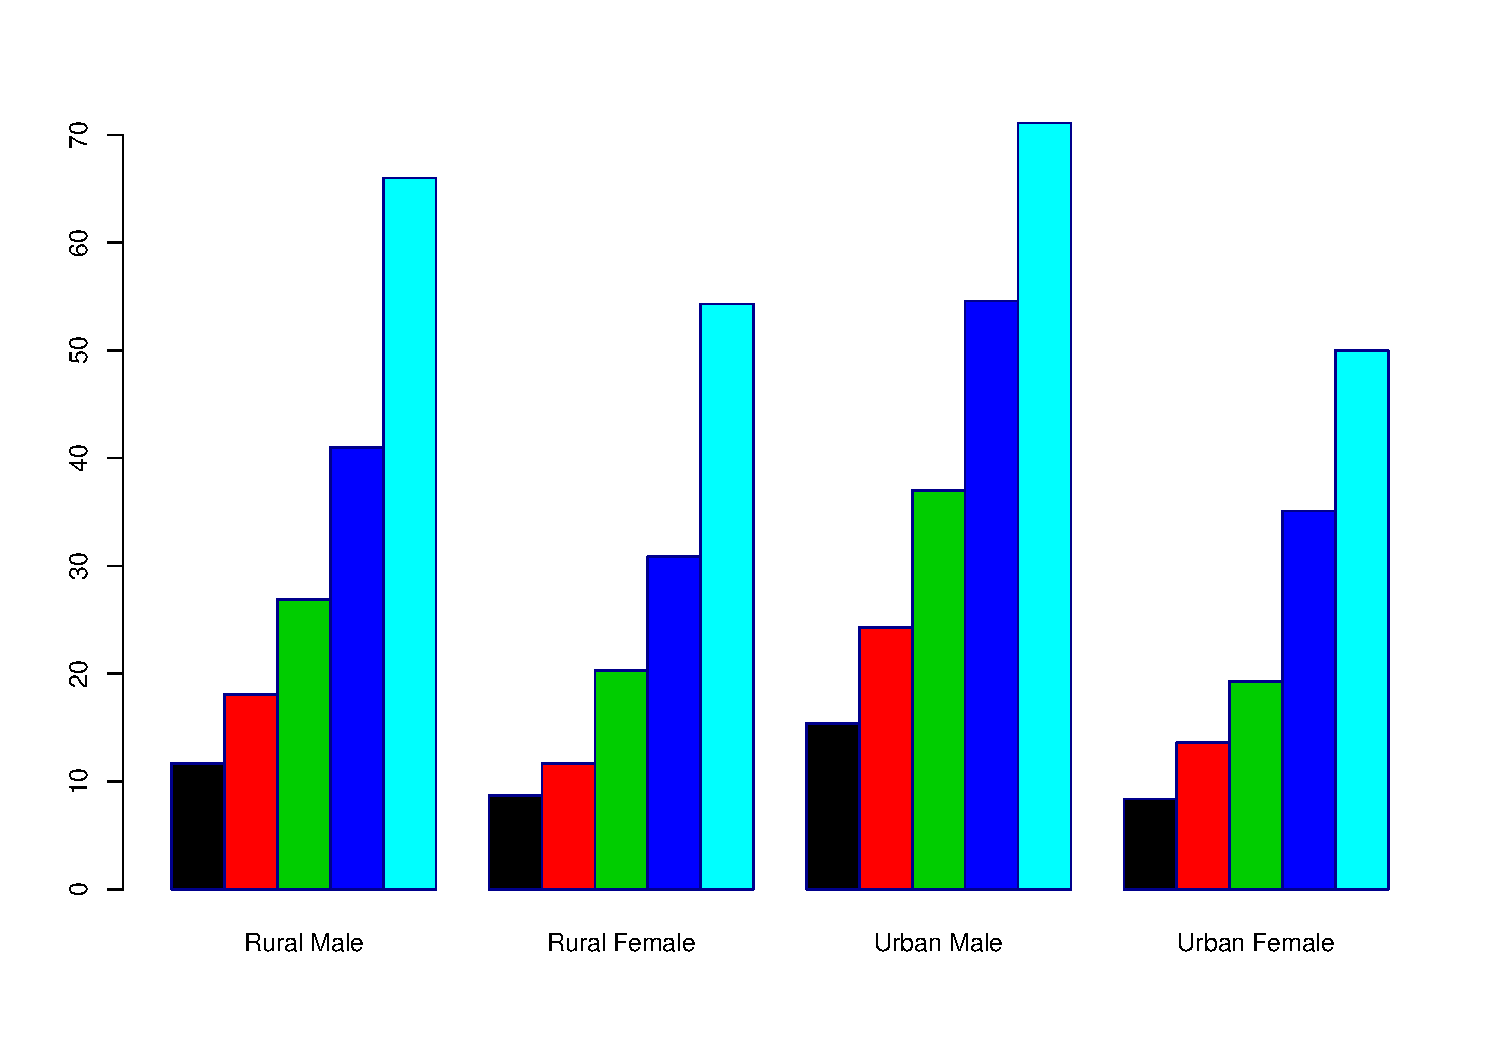
\includegraphics{R_intern_files/figure-beamer/unnamed-chunk-162-1.pdf}

\end{frame}

\begin{frame}[fragile]{Einfacher Scatterplot III}

\begin{Shaded}
\begin{Highlighting}[]
\KeywordTok{plot}\NormalTok{(x,y,}\DataTypeTok{pch=}\DecValTok{20}\NormalTok{)}
\end{Highlighting}
\end{Shaded}

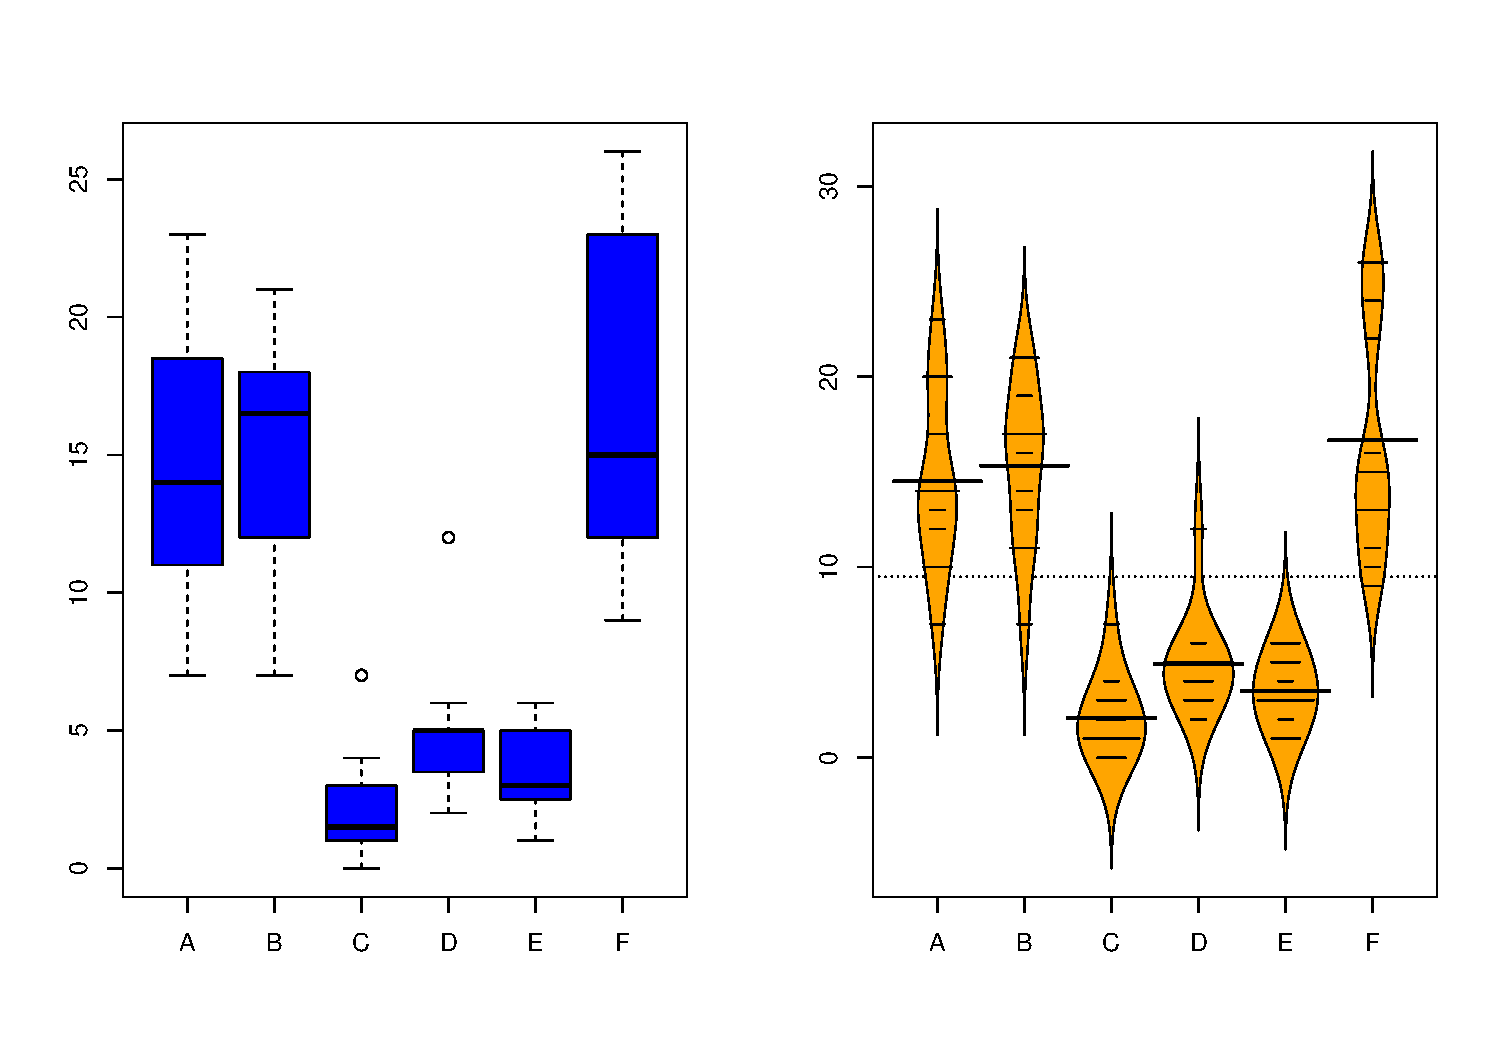
\includegraphics{R_intern_files/figure-beamer/unnamed-chunk-163-1.pdf}

\end{frame}

\begin{frame}[fragile]{Boxplot}

\begin{itemize}
\tightlist
\item
  Einen einfachen Boxplot erstellt man mit \texttt{boxplot()}
\item
  Auch \texttt{boxplot()} muss mindestens ein Beobachtungsvektor
  übergeben werden
\end{itemize}

\begin{Shaded}
\begin{Highlighting}[]
\NormalTok{?boxplot}
\end{Highlighting}
\end{Shaded}

\end{frame}

\begin{frame}[fragile]{Horizontaler Boxplot}

\begin{Shaded}
\begin{Highlighting}[]
\KeywordTok{boxplot}\NormalTok{(Chem97$gcsescore,}
\DataTypeTok{horizontal=}\OtherTok{TRUE}\NormalTok{)}
\end{Highlighting}
\end{Shaded}

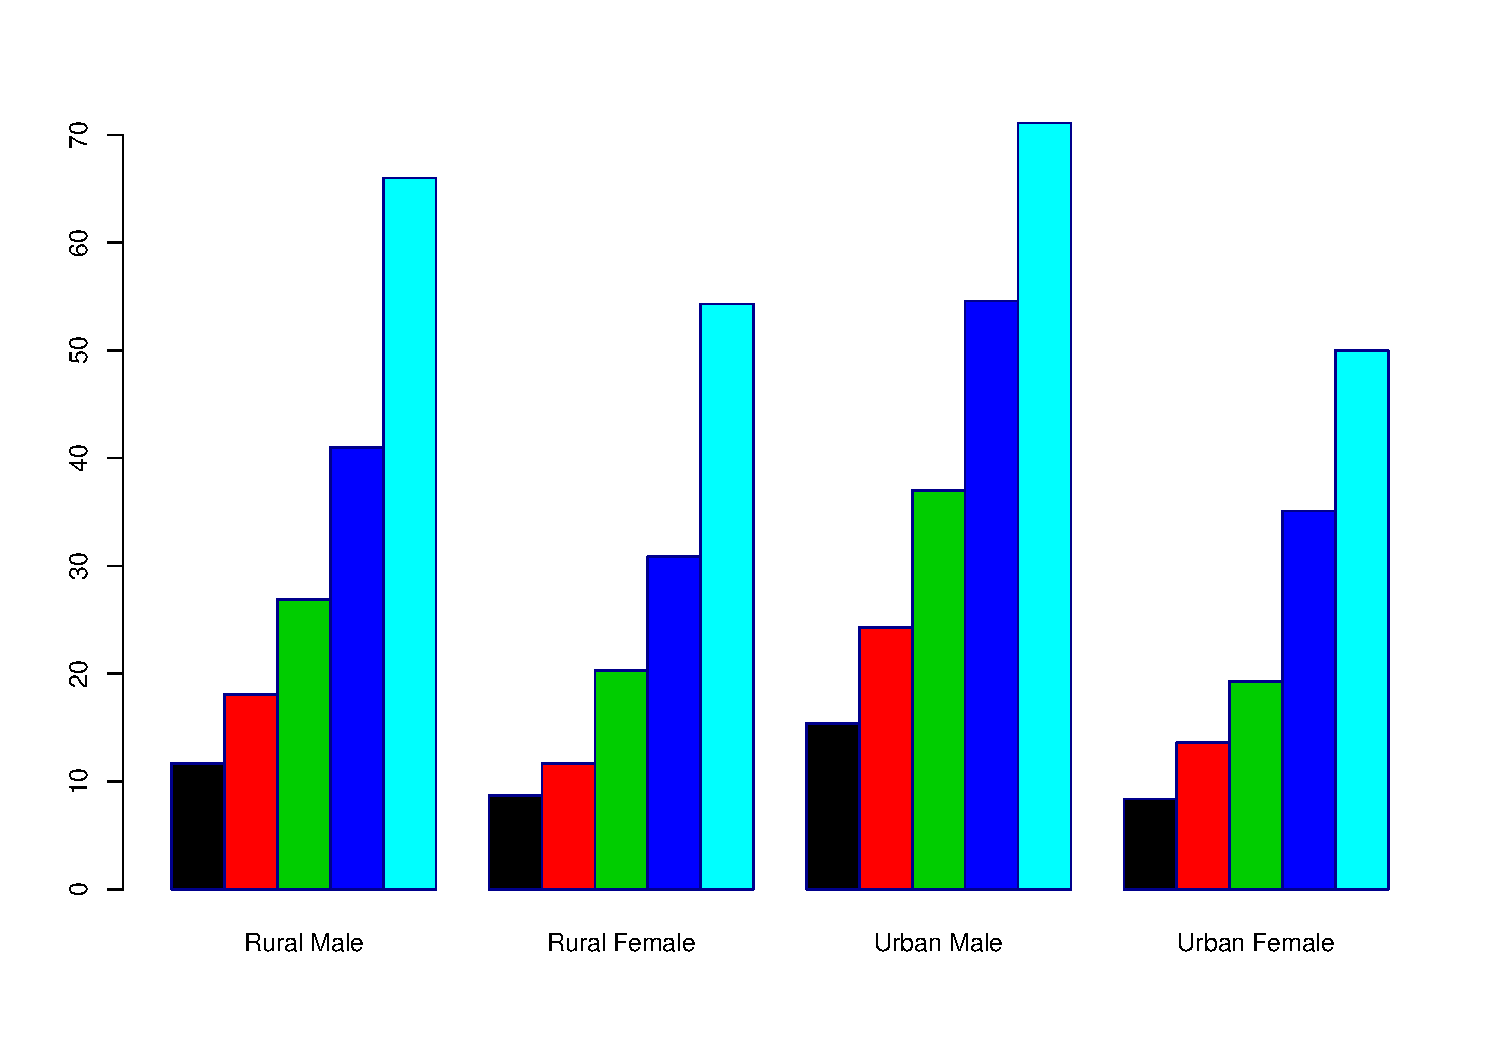
\includegraphics{R_intern_files/figure-beamer/unnamed-chunk-165-1.pdf}

\begin{itemize}
\tightlist
\item
  \href{http://edoc.hu-berlin.de/dissertationen/gruenwald-andreas-2005-01-17/HTML/chapter2.html}{Erklärung
  zu Boxplots}
\end{itemize}

\end{frame}

\begin{frame}[fragile]{Gruppierte Boxplots}

\begin{itemize}
\tightlist
\item
  Ein sehr einfacher Weg, einen ersten Eindruck über bedingte
  Verteilungen zu bekommen ist über sog. Gruppierte notched Boxplots
\item
  Dazu muss der Funktion \texttt{boxplot()} ein sog. Formel-Objekt
  übergeben werden
\item
  Die bedingende Variable steht dabei auf der rechten Seite einer Tilde
\end{itemize}

\end{frame}

\begin{frame}[fragile]{Beispiel grupierter Boxplot}

\begin{Shaded}
\begin{Highlighting}[]
\KeywordTok{boxplot}\NormalTok{(Chem97$gcsescore~Chem97$gender)}
\end{Highlighting}
\end{Shaded}

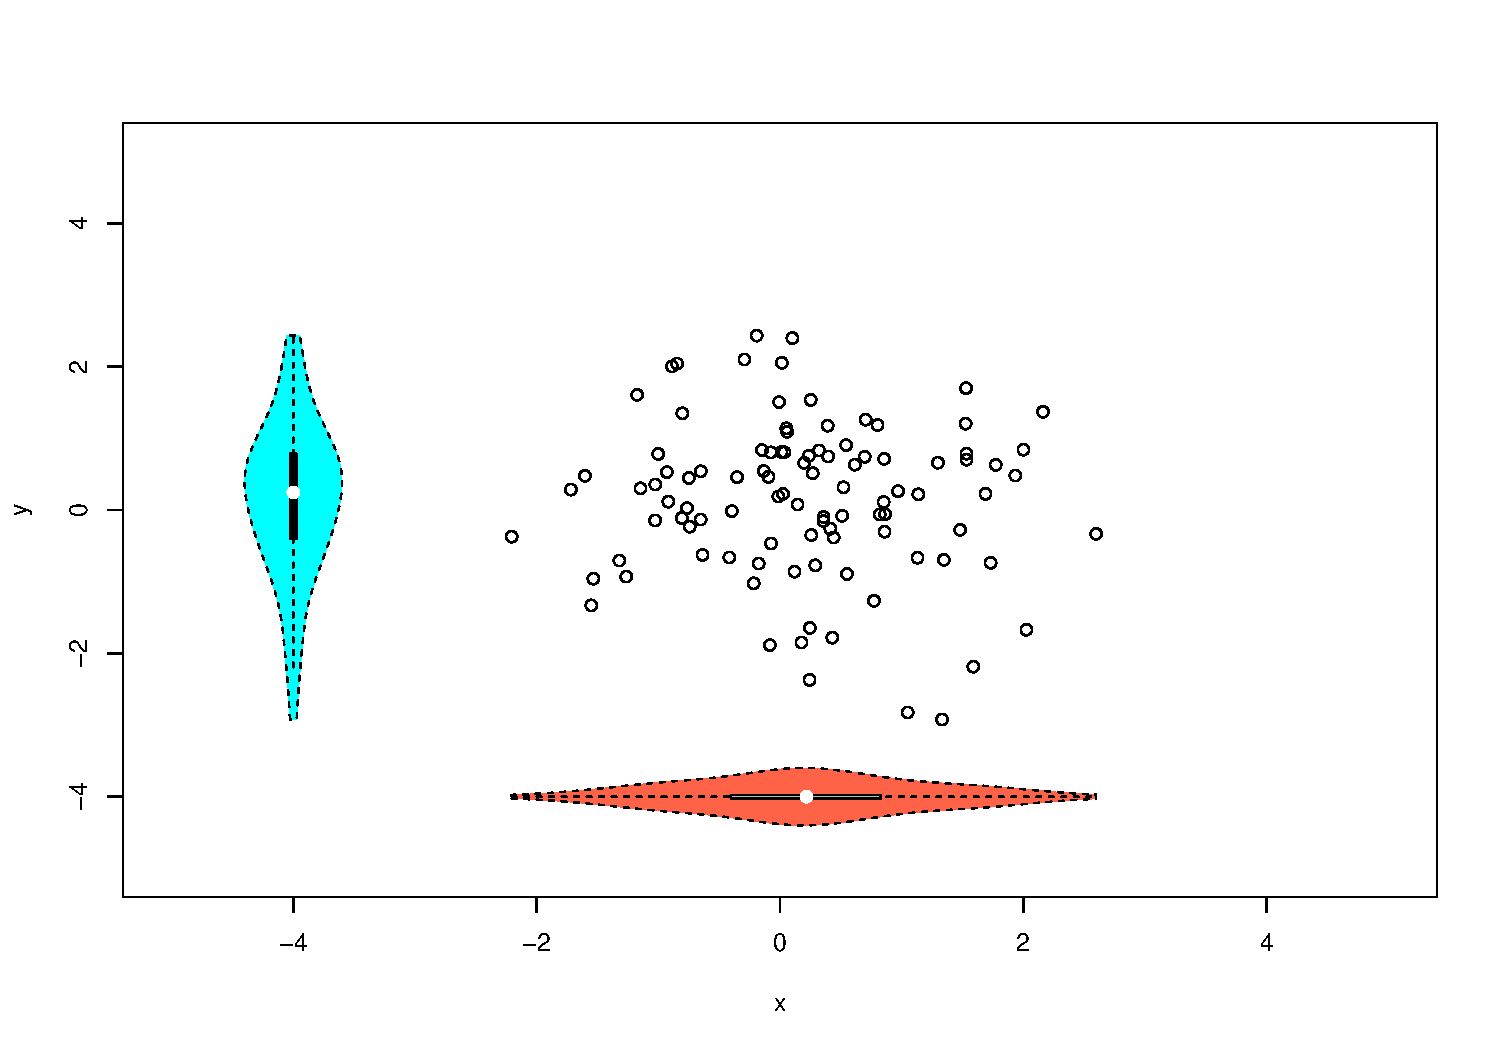
\includegraphics{R_intern_files/figure-beamer/unnamed-chunk-166-1.pdf}

\end{frame}

\begin{frame}[fragile]{Alternativen zu Boxplot}

Violinplot

\begin{itemize}
\tightlist
\item
  Baut auf Boxplot auf
\item
  Zusätzlich Informationen über Dichte der Daten
\item
  Dichte wird über Kernel Methode berechnet.
\item
  weißer Punkt - Median
\item
  Je weiter die Ausdehnung, desto größer ist die Dichte an dieser
  Stelle.
\end{itemize}

\begin{Shaded}
\begin{Highlighting}[]
\CommentTok{# Beispieldaten erzeugen}
\NormalTok{x <-}\StringTok{ }\KeywordTok{rnorm}\NormalTok{(}\DecValTok{100}\NormalTok{)}
\NormalTok{y <-}\StringTok{ }\KeywordTok{rnorm}\NormalTok{(}\DecValTok{100}\NormalTok{)}
\end{Highlighting}
\end{Shaded}

\end{frame}

\begin{frame}[fragile]{Die Bibliothek \texttt{vioplot}}

\begin{Shaded}
\begin{Highlighting}[]
\KeywordTok{library}\NormalTok{(vioplot)}
\KeywordTok{plot}\NormalTok{(x, y, }\DataTypeTok{xlim=}\KeywordTok{c}\NormalTok{(-}\DecValTok{5}\NormalTok{,}\DecValTok{5}\NormalTok{), }\DataTypeTok{ylim=}\KeywordTok{c}\NormalTok{(-}\DecValTok{5}\NormalTok{,}\DecValTok{5}\NormalTok{))}
\KeywordTok{vioplot}\NormalTok{(x, }\DataTypeTok{col=}\StringTok{"tomato"}\NormalTok{, }\DataTypeTok{horizontal=}\OtherTok{TRUE}\NormalTok{, }\DataTypeTok{at=}\NormalTok{-}\DecValTok{4}\NormalTok{, }
        \DataTypeTok{add=}\OtherTok{TRUE}\NormalTok{,}\DataTypeTok{lty=}\DecValTok{2}\NormalTok{, }\DataTypeTok{rectCol=}\StringTok{"gray"}\NormalTok{)}
\KeywordTok{vioplot}\NormalTok{(y, }\DataTypeTok{col=}\StringTok{"cyan"}\NormalTok{, }\DataTypeTok{horizontal=}\OtherTok{FALSE}\NormalTok{, }\DataTypeTok{at=}\NormalTok{-}\DecValTok{4}\NormalTok{, }
        \DataTypeTok{add=}\OtherTok{TRUE}\NormalTok{,}\DataTypeTok{lty=}\DecValTok{2}\NormalTok{)}
\end{Highlighting}
\end{Shaded}

\end{frame}

\begin{frame}{\texttt{vioplot} - Das Ergebnis}

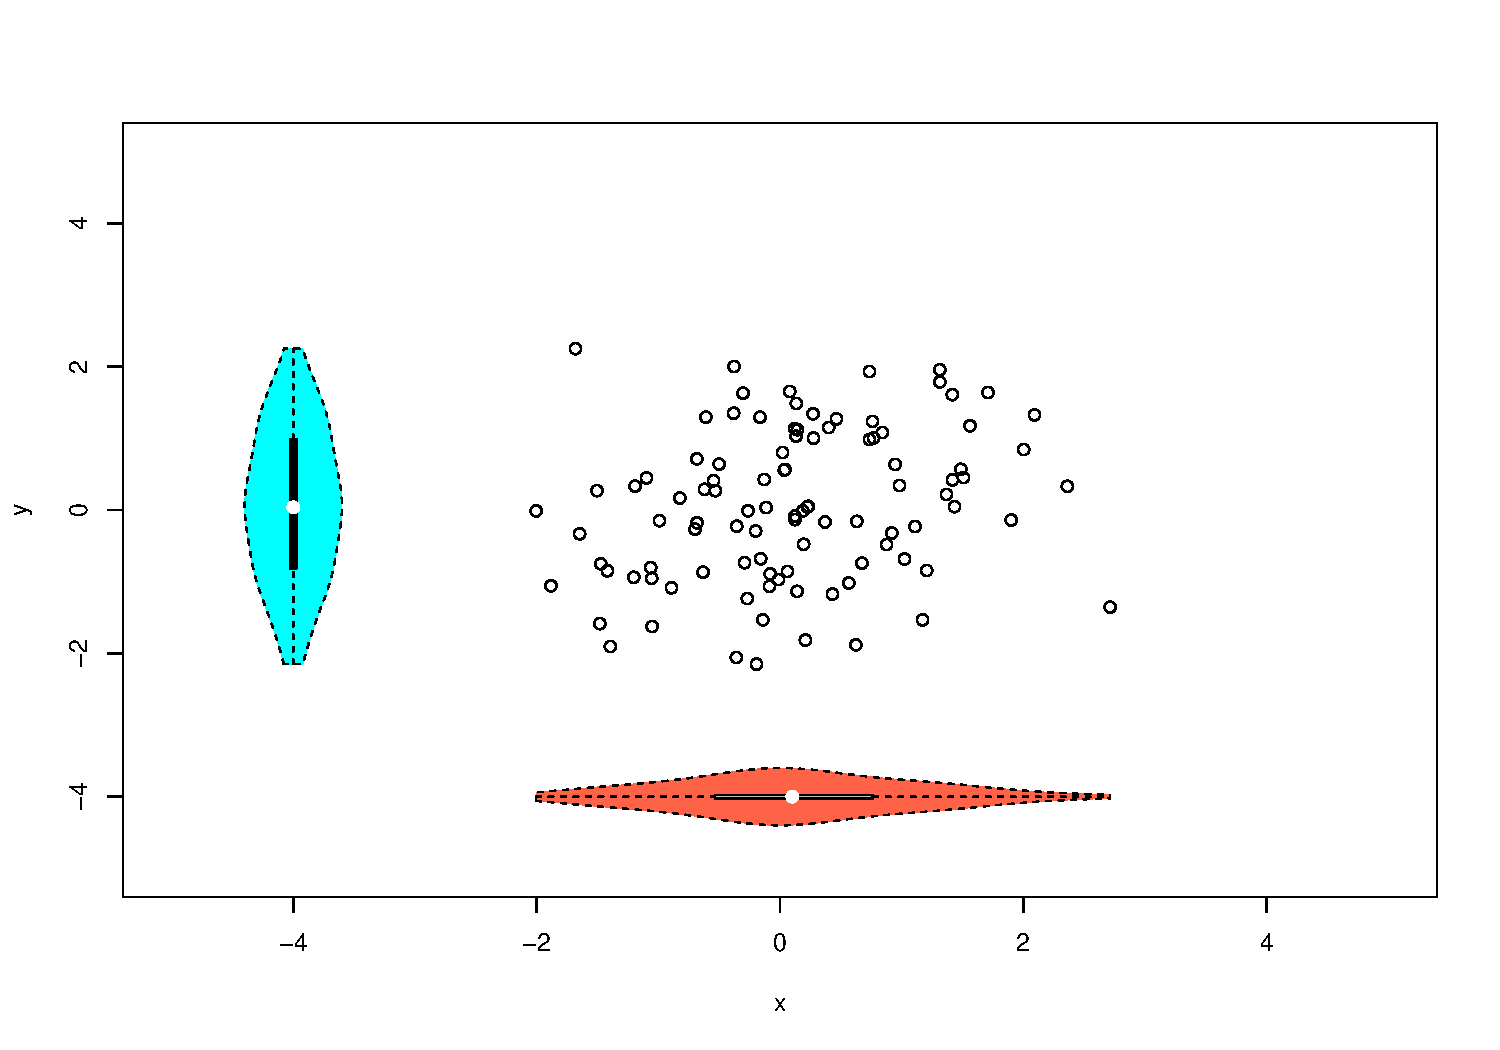
\includegraphics{R_intern_files/figure-beamer/unnamed-chunk-169-1.pdf}

\end{frame}

\begin{frame}[fragile]{Alternativen zum Boxplot}

\begin{Shaded}
\begin{Highlighting}[]
\KeywordTok{library}\NormalTok{(beanplot)}
\KeywordTok{par}\NormalTok{(}\DataTypeTok{mfrow =} \KeywordTok{c}\NormalTok{(}\DecValTok{1}\NormalTok{,}\DecValTok{2}\NormalTok{))}
\KeywordTok{boxplot}\NormalTok{(count~spray,}\DataTypeTok{data=}\NormalTok{InsectSprays,}\DataTypeTok{col=}\StringTok{"blue"}\NormalTok{)}
\KeywordTok{beanplot}\NormalTok{(count~spray,}\DataTypeTok{data=}\NormalTok{InsectSprays,}\DataTypeTok{col=}\StringTok{"orange"}\NormalTok{)}
\end{Highlighting}
\end{Shaded}

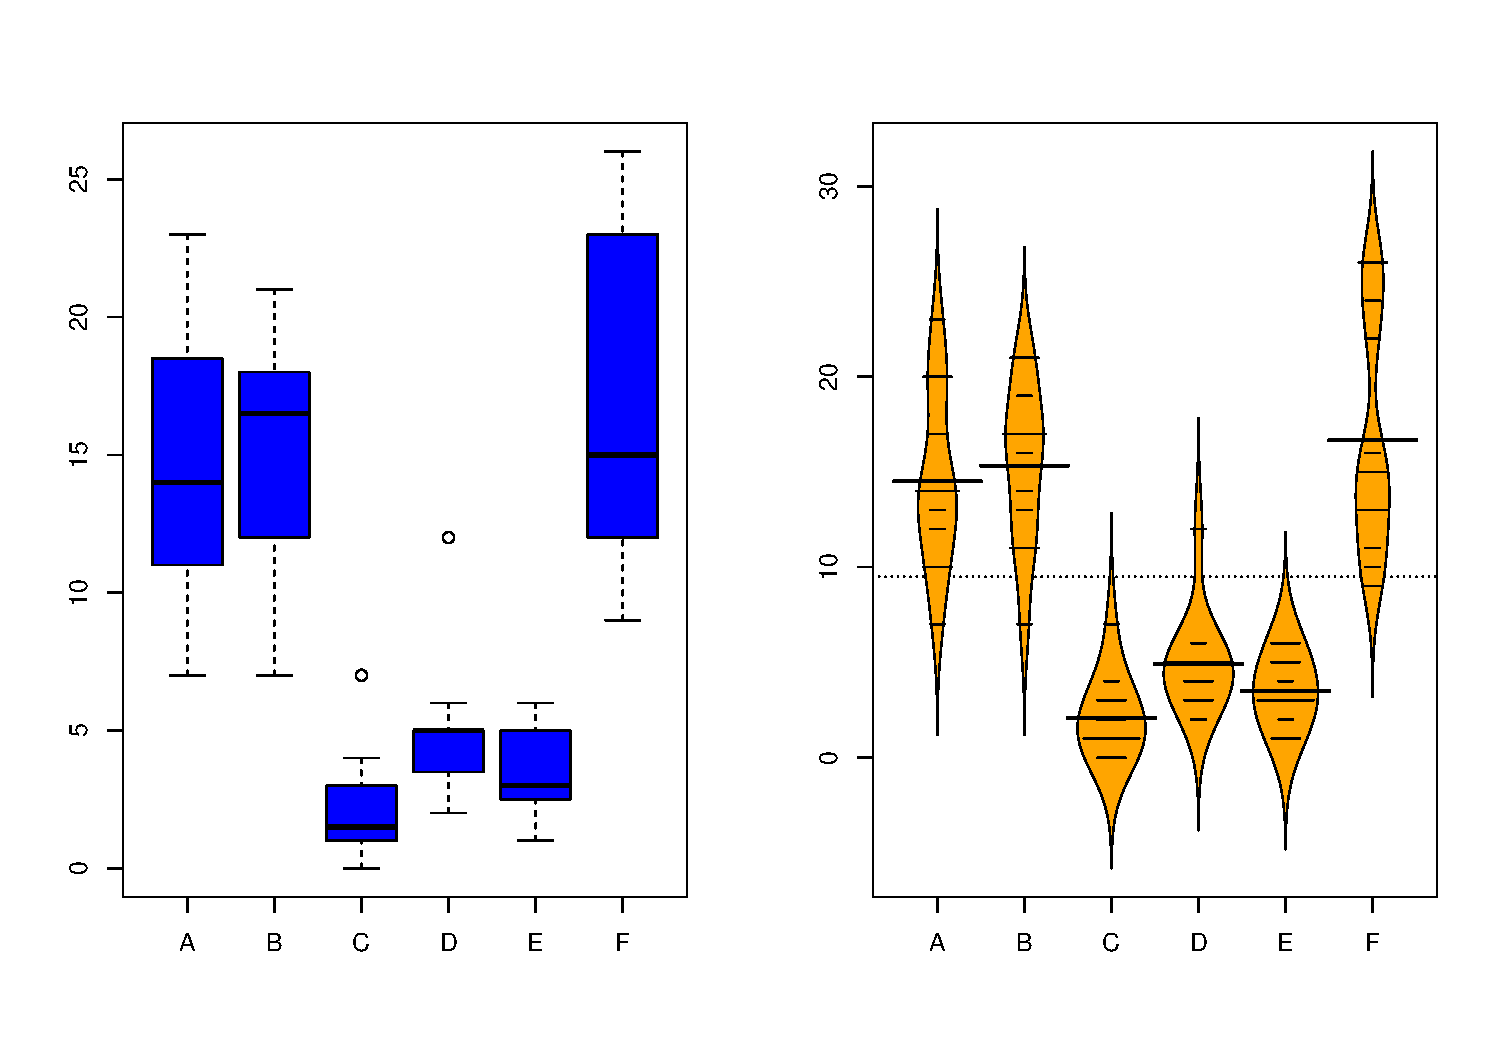
\includegraphics{R_intern_files/figure-beamer/unnamed-chunk-170-1.pdf}

\end{frame}

\begin{frame}[fragile]{\href{https://www.r-bloggers.com/draw-figures-in-cmyk-mode-in-r/}{CMYK
Farbschema}}

\begin{Shaded}
\begin{Highlighting}[]
\KeywordTok{pdf}\NormalTok{(}\StringTok{"test.cmyk.pdf"}\NormalTok{, }\DataTypeTok{colormodel=}\StringTok{'cmyk'}\NormalTok{)}
\KeywordTok{pie}\NormalTok{(}\DecValTok{1}\NormalTok{:}\DecValTok{10}\NormalTok{, }\DataTypeTok{col=}\DecValTok{1}\NormalTok{:}\DecValTok{10}\NormalTok{)}
\KeywordTok{dev.off}\NormalTok{() }
\end{Highlighting}
\end{Shaded}

\end{frame}

\begin{frame}[fragile]{Aufgabe - einfache Grafiken}

\begin{itemize}
\tightlist
\item
  Laden Sie den Datensatz \texttt{VADeaths} und erzeugen Sie den
  folgenden plot:
\end{itemize}

\includegraphics{R_intern_files/figure-beamer/unnamed-chunk-172-1.pdf}

\end{frame}

\begin{frame}{Datenanalyse}

\end{frame}

\begin{frame}[fragile]{Den Datensatz laden}

\begin{verbatim}
## Warning: NAs durch Umwandlung erzeugt
\end{verbatim}

\begin{Shaded}
\begin{Highlighting}[]
\KeywordTok{library}\NormalTok{(foreign)}
\NormalTok{dat <-}\StringTok{ }\KeywordTok{read.dta}\NormalTok{(}
\StringTok{"https://github.com/Japhilko/RSocialScience/blob/master/data/}
\StringTok{GPanel.dta?raw=true"}\NormalTok{)}
\NormalTok{dat$bazq020a <-}\StringTok{ }\KeywordTok{as.numeric}\NormalTok{(dat$bazq020a)}
\end{Highlighting}
\end{Shaded}

\end{frame}

\begin{frame}[fragile]{Streuungsmaße}

\begin{itemize}
\tightlist
\item
  Varianz: \texttt{var()}
\item
  Standardabweichung: \texttt{sd()}
\item
  Minimum und Maximum: \texttt{min()} und \texttt{max()}
\item
  Range: \texttt{range()}
\end{itemize}

\begin{Shaded}
\begin{Highlighting}[]
\KeywordTok{var}\NormalTok{(dat$bazq020a)}
\end{Highlighting}
\end{Shaded}

\begin{verbatim}
## [1] NA
\end{verbatim}

\begin{Shaded}
\begin{Highlighting}[]
\KeywordTok{var}\NormalTok{(dat$bazq020a,}\DataTypeTok{na.rm=}\NormalTok{T)}
\end{Highlighting}
\end{Shaded}

\begin{verbatim}
## [1] 476.8859
\end{verbatim}

\begin{Shaded}
\begin{Highlighting}[]
\KeywordTok{sd}\NormalTok{(dat$bazq020a,}\DataTypeTok{na.rm=}\NormalTok{T)}
\end{Highlighting}
\end{Shaded}

\begin{verbatim}
## [1] 21.83772
\end{verbatim}

\begin{Shaded}
\begin{Highlighting}[]
\KeywordTok{range}\NormalTok{(dat$bazq020a,}\DataTypeTok{na.rm=}\NormalTok{T)}
\end{Highlighting}
\end{Shaded}

\begin{verbatim}
## [1] -99  45
\end{verbatim}

\end{frame}

\begin{frame}[fragile]{Häufigkeiten und gruppierte Kennwerte}

\begin{itemize}
\tightlist
\item
  Eine Auszählung der Häufigkeiten der Merkmale einer Variable liefert
  \texttt{table()}
\item
  Mit \texttt{table()} sind auch Kreuztabellierungen möglich indem zwei
  Variablen durch Komma getrennt werden: \texttt{table(x,y)} liefert
  Häufigkeiten von \texttt{y} für gegebene Ausprägungen von \texttt{x}
\end{itemize}

\begin{Shaded}
\begin{Highlighting}[]
\KeywordTok{table}\NormalTok{(dat$a11d054a)}
\end{Highlighting}
\end{Shaded}

\begin{verbatim}
## 
## Männlich Weiblich 
##       43       57
\end{verbatim}

\end{frame}

\begin{frame}[fragile]{Tabellieren - weiteres Beispiel}

\begin{Shaded}
\begin{Highlighting}[]
\NormalTok{?table}
\end{Highlighting}
\end{Shaded}

\begin{Shaded}
\begin{Highlighting}[]
\KeywordTok{table}\NormalTok{(dat$a11d054a)}
\end{Highlighting}
\end{Shaded}

\begin{verbatim}
## 
## Männlich Weiblich 
##       43       57
\end{verbatim}

\begin{Shaded}
\begin{Highlighting}[]
\KeywordTok{table}\NormalTok{(dat$a11d054a,dat$a11d056z)}
\end{Highlighting}
\end{Shaded}

\begin{verbatim}
##           
##            Ambiguous answer Item nonresponse Not reached Unit nonresponse
##   Männlich                0                0           0                0
##   Weiblich                0                0           0                0
##           
##            Not in panel 18 bis unter 20 Jahre 20 bis unter 25 Jahre
##   Männlich            0                     2                     2
##   Weiblich            0                     2                     4
##           
##            25 bis unter 30 Jahre 30 bis unter 35 Jahre
##   Männlich                     2                     3
##   Weiblich                     5                     2
##           
##            35 bis unter 40 Jahre 40 bis unter 45 Jahre
##   Männlich                     2                     1
##   Weiblich                     4                     4
##           
##            45 bis unter 50 Jahre 50 bis unter 55 Jahre
##   Männlich                     8                     9
##   Weiblich                     6                     7
##           
##            55 bis unter 60 Jahre 60 bis unter 63 Jahre
##   Männlich                     3                     2
##   Weiblich                     5                     9
##           
##            63 bis unter 65 Jahre 65 bis unter 70 Jahre 70 Jahre und Älter
##   Männlich                     3                     5                  1
##   Weiblich                     1                     5                  3
\end{verbatim}

\end{frame}

\begin{frame}[fragile]{Häufigkeitstabellen}

\begin{itemize}
\tightlist
\item
  \texttt{prop.table()} liefert die relativen Häufigkeiten
\item
  Wird die Funktion außerhalb einer \texttt{table()} Funktion
  geschrieben erhält man die relativen Häufigkeiten bezogen auf alle
  Zellen
\end{itemize}

\end{frame}

\begin{frame}[fragile]{Die Funktion \texttt{prop.table}}

\begin{Shaded}
\begin{Highlighting}[]
\NormalTok{?prop.table}
\end{Highlighting}
\end{Shaded}

\begin{Shaded}
\begin{Highlighting}[]
\KeywordTok{prop.table}\NormalTok{(}\KeywordTok{table}\NormalTok{(dat$a11d054a,dat$a11d056z),}\DecValTok{1}\NormalTok{)}
\end{Highlighting}
\end{Shaded}

\begin{verbatim}
##           
##            Ambiguous answer Item nonresponse Not reached Unit nonresponse
##   Männlich       0.00000000       0.00000000  0.00000000       0.00000000
##   Weiblich       0.00000000       0.00000000  0.00000000       0.00000000
##           
##            Not in panel 18 bis unter 20 Jahre 20 bis unter 25 Jahre
##   Männlich   0.00000000            0.04651163            0.04651163
##   Weiblich   0.00000000            0.03508772            0.07017544
##           
##            25 bis unter 30 Jahre 30 bis unter 35 Jahre
##   Männlich            0.04651163            0.06976744
##   Weiblich            0.08771930            0.03508772
##           
##            35 bis unter 40 Jahre 40 bis unter 45 Jahre
##   Männlich            0.04651163            0.02325581
##   Weiblich            0.07017544            0.07017544
##           
##            45 bis unter 50 Jahre 50 bis unter 55 Jahre
##   Männlich            0.18604651            0.20930233
##   Weiblich            0.10526316            0.12280702
##           
##            55 bis unter 60 Jahre 60 bis unter 63 Jahre
##   Männlich            0.06976744            0.04651163
##   Weiblich            0.08771930            0.15789474
##           
##            63 bis unter 65 Jahre 65 bis unter 70 Jahre 70 Jahre und Älter
##   Männlich            0.06976744            0.11627907         0.02325581
##   Weiblich            0.01754386            0.08771930         0.05263158
\end{verbatim}

\end{frame}

\begin{frame}[fragile]{Die aggregate Funktion}

\begin{itemize}
\tightlist
\item
  Mit der \texttt{aggregate()} Funktion können Kennwerte für
  Untergruppen erstellt werden
\item
  \texttt{aggregate(x,by,FUN)} müssen mindestens drei Argumente
  übergeben werden:
\end{itemize}

\begin{Shaded}
\begin{Highlighting}[]
\KeywordTok{aggregate}\NormalTok{(dat$bazq020a,}\DataTypeTok{by=}\KeywordTok{list}\NormalTok{(dat$a11d054a),mean,}\DataTypeTok{na.rm=}\NormalTok{T)}
\end{Highlighting}
\end{Shaded}

\begin{verbatim}
##    Group.1         x
## 1 Männlich 13.534884
## 2 Weiblich  8.773585
\end{verbatim}

\texttt{x}: ein oder mehrere Beobachtungsvektor(en) für den der Kennwert
berechnet werden soll

\texttt{by}: eine oder mehrere bedingende Variable(n)

\texttt{FUN}: die Funktion welche den Kennwert berechnet (z.B.
\texttt{mean} oder \texttt{sd})

\end{frame}

\begin{frame}[fragile]{Beispieldatensatz - apply Funktion}

\begin{Shaded}
\begin{Highlighting}[]
\NormalTok{ApplyDat <-}\StringTok{ }\KeywordTok{array}\NormalTok{(}\DecValTok{1}\NormalTok{:}\DecValTok{8}\NormalTok{,}\KeywordTok{c}\NormalTok{(}\DecValTok{4}\NormalTok{,}\DecValTok{2}\NormalTok{))}
\end{Highlighting}
\end{Shaded}

\begin{verbatim}
##      [,1] [,2]
## [1,]    1    5
## [2,]    2    6
## [3,]    3    7
## [4,]    4    8
\end{verbatim}

\end{frame}

\begin{frame}[fragile]{Argumente der Funktion apply}

\begin{Shaded}
\begin{Highlighting}[]
\NormalTok{?apply}
\end{Highlighting}
\end{Shaded}

\begin{itemize}
\item
  Für \texttt{margin=1} die Funktion \texttt{mean} auf die Reihen
  angewendet,
\item
  Für \texttt{margin=2} die Funktion \texttt{mean} auf die Spalten
  angewendet,
\item
  Anstatt \texttt{mean} können auch andere Funktionen wie \texttt{var},
  \texttt{sd} oder \texttt{length} verwendet werden.
\end{itemize}

\end{frame}

\begin{frame}[fragile]{Die \texttt{apply} Funktion anwenden}

\begin{Shaded}
\begin{Highlighting}[]
\KeywordTok{apply}\NormalTok{(ApplyDat,}\DecValTok{1}\NormalTok{,mean)}
\end{Highlighting}
\end{Shaded}

\begin{verbatim}
## [1] 3 4 5 6
\end{verbatim}

\begin{Shaded}
\begin{Highlighting}[]
\KeywordTok{apply}\NormalTok{(ApplyDat,}\DecValTok{2}\NormalTok{,mean)}
\end{Highlighting}
\end{Shaded}

\begin{verbatim}
## [1] 2.5 6.5
\end{verbatim}

\end{frame}

\begin{frame}[fragile]{Die Funktion apply}

\begin{Shaded}
\begin{Highlighting}[]
\KeywordTok{apply}\NormalTok{(ApplyDat,}\DecValTok{1}\NormalTok{,var)}
\end{Highlighting}
\end{Shaded}

\begin{verbatim}
## [1] 8 8 8 8
\end{verbatim}

\begin{Shaded}
\begin{Highlighting}[]
\KeywordTok{apply}\NormalTok{(ApplyDat,}\DecValTok{1}\NormalTok{,sd)}
\end{Highlighting}
\end{Shaded}

\begin{verbatim}
## [1] 2.828427 2.828427 2.828427 2.828427
\end{verbatim}

\begin{Shaded}
\begin{Highlighting}[]
\KeywordTok{apply}\NormalTok{(ApplyDat,}\DecValTok{1}\NormalTok{,range)}
\end{Highlighting}
\end{Shaded}

\begin{verbatim}
##      [,1] [,2] [,3] [,4]
## [1,]    1    2    3    4
## [2,]    5    6    7    8
\end{verbatim}

\begin{Shaded}
\begin{Highlighting}[]
\KeywordTok{apply}\NormalTok{(ApplyDat,}\DecValTok{1}\NormalTok{,length)}
\end{Highlighting}
\end{Shaded}

\begin{verbatim}
## [1] 2 2 2 2
\end{verbatim}

\end{frame}

\begin{frame}[fragile]{Die Funktion tapply}

\begin{Shaded}
\begin{Highlighting}[]
\NormalTok{?tapply}
\end{Highlighting}
\end{Shaded}

\begin{itemize}
\tightlist
\item
  Auch andere Funktionen können eingesetzt werden\ldots{}. - Auch selbst
  programmierte Funktionen
\item
  Im Beispiel wird die einfachste eigene Funktion angewendet.
\end{itemize}

\end{frame}

\begin{frame}[fragile]{Beispieldaten Funktion \texttt{tapply}}

\begin{Shaded}
\begin{Highlighting}[]
\NormalTok{tapdat <-}\StringTok{ }\KeywordTok{data.frame}\NormalTok{(}\DataTypeTok{SEX=}\KeywordTok{sample}\NormalTok{(}\KeywordTok{c}\NormalTok{(}\StringTok{"m"}\NormalTok{,}\StringTok{"w"}\NormalTok{),}\DecValTok{10}\NormalTok{,}\DataTypeTok{replace=}\NormalTok{T),}\DataTypeTok{INC=}\KeywordTok{rnorm}\NormalTok{(}\DecValTok{10}\NormalTok{))}
\end{Highlighting}
\end{Shaded}

\begin{longtable}[]{@{}lr@{}}
\toprule
SEX & INC\tabularnewline
\midrule
\endhead
w & 0.0900102\tabularnewline
m & -1.8207756\tabularnewline
m & 0.6186499\tabularnewline
w & 0.6927763\tabularnewline
w & -1.4438957\tabularnewline
w & 0.9669492\tabularnewline
\bottomrule
\end{longtable}

\end{frame}

\begin{frame}[fragile]{Beispiel Funktion tapply}

\begin{Shaded}
\begin{Highlighting}[]
\KeywordTok{tapply}\NormalTok{(tapdat$INC,tapdat$SEX,mean)}
\end{Highlighting}
\end{Shaded}

\begin{verbatim}
##          m          w 
## 0.07421522 0.07646000
\end{verbatim}

\end{frame}

\begin{frame}{Aufgabe - apply Funktion anwenden}

\begin{itemize}
\item
  Erstellen Sie eine Matrix A mit 4 Zeilen und 25 Spalten, die die Werte
  1 bis 100 enthält. Analog dazu erstellen Sie eine Matrix B mit 25
  Zeilen und 4 Spalten, die die Werte 1 bis 100 enthält.
\item
  Berechnen Sie mittels dem apply()-Befehl den Mittelwert und die
  Varianz für jede Zeile von A bzw. B.
\item
  Berechnen Sie mittels dem apply()-Befehl den Mittelwert und die
  Varianz für jede Spalte von A bzw. B.
\end{itemize}

\end{frame}

\begin{frame}[fragile]{Links Datenanalyse}

\begin{itemize}
\item
  Die Benutzung von \texttt{apply}, \texttt{tapply}, etc. (Artikel bei
  \href{http://www.r-bloggers.com/using-apply-sapply-lapply-in-r/}{R-bloggers})
\item
  \href{http://www.statmethods.net/stats/descriptives.html}{Quick-R zu
  deskriptiver Statistik}
\item
  \href{http://www.statmethods.net/management/aggregate.html}{Quick-R
  zur Funktion \texttt{aggregate}}
\end{itemize}

\end{frame}

\begin{frame}{Grafiken und Zusammenhang}

\end{frame}

\begin{frame}{Ein Plot sagt mehr als 1000 Worte}

\begin{itemize}
\tightlist
\item
  Grafisch gestützte Datenanalyse ist toll
\item
  Gute Plots können zu einem besseren Verständnis beitragen
\item
  Einen Plot zu generieren geht schnell
\item
  Einen guten Plot zu machen kann sehr lange dauern
\item
  Mit R Plots zu generieren macht Spaß
\item
  Mit R erstellte Plots haben hohe Qualität
\item
  Fast jeder Plottyp wird von R unterstützt
\item
  R kennt eine große Menge an Exportformaten für Grafiken
\end{itemize}

\end{frame}

\begin{frame}{Plot ist nicht gleich Plot}

\begin{itemize}
\tightlist
\item
  Bereits das base Package bringt eine große Menge von Plot Funktionen
  mit
\item
  Das lattice Packet erweitert dessen Funktionalität
\item
  Eine weit über diese Einführung hinausgehende Übersicht findet sich in
  Murrell, P (2006): R Graphics.
\end{itemize}

\end{frame}

\begin{frame}{Task View zu Thema
\href{https://cran.r-project.org/web/views/Graphics.html}{Graphiken}}

\includegraphics{./tex2pdf.956/5e4adb82cb6141da7bafecd33dfdc7d0e44f95dc.png}

\end{frame}

\begin{frame}[fragile]{Datensatz}

\begin{Shaded}
\begin{Highlighting}[]
\KeywordTok{library}\NormalTok{(mlmRev)}
\KeywordTok{data}\NormalTok{(Chem97)}
\end{Highlighting}
\end{Shaded}

\begin{itemize}
\tightlist
\item
  {[}lea{]} Local Education Authority - a factor
\item
  {[}school{]} School identifier - a factor
\item
  {[}student{]} Student identifier - a factor
\item
  {[}score{]} Point score on A-level Chemistry in 1997
\item
  {[}gender{]} Student's gender
\item
  {[}age{]} Age in month, centred at 222 months or 18.5 years
\item
  {[}gcsescore{]} Average GCSE score of individual.
\item
  {[}gcsecnt{]} Average GCSE score of individual, centered at mean.
\end{itemize}

\end{frame}

\begin{frame}[fragile]{Histogramm - Die Funktion hist()}

Wir erstellen ein Histogramm der Variable gcsescore (Hilfe mit
\texttt{?hist}):

\begin{Shaded}
\begin{Highlighting}[]
\KeywordTok{hist}\NormalTok{(Chem97$gcsescore)}
\end{Highlighting}
\end{Shaded}

\includegraphics{R_intern_files/figure-beamer/unnamed-chunk-198-1.pdf}

\end{frame}

\begin{frame}{Graphik speichern}

\begin{itemize}
\tightlist
\item
  Mit dem button Export in Rstudio kann man die Grafik speichern.
\end{itemize}

\includegraphics{./tex2pdf.956/c841157f024cc7a3d01009eeb5c876036fad5d81.png}

\end{frame}

\begin{frame}[fragile]{Befehl um Graphik zu speichern}

\begin{itemize}
\tightlist
\item
  Alternativ auch bspw. mit den Befehlen \texttt{png}, \texttt{pdf} oder
  \texttt{jpeg}
\end{itemize}

\begin{Shaded}
\begin{Highlighting}[]
\KeywordTok{png}\NormalTok{(}\StringTok{"Histogramm.png"}\NormalTok{)}
\KeywordTok{hist}\NormalTok{(Chem97$gcsescore)}
\KeywordTok{dev.off}\NormalTok{()}
\end{Highlighting}
\end{Shaded}

\end{frame}

\begin{frame}[fragile]{Histogramme}

\begin{itemize}
\tightlist
\item
  Die Funktion \texttt{hist()} plottet ein Histogramm der Daten
\item
  Der Funktion muss mindestens ein Beobachtungsvektor übergeben werden
\item
  \texttt{hist()} hat noch sehr viel mehr Argumente, die alle
  (sinnvolle) default values haben
\end{itemize}

\begin{longtable}[]{@{}lll@{}}
\toprule
Argument & Bedeutung & Beispiel\tabularnewline
\midrule
\endhead
main & Überschrift & main=``Hallo Welt''\tabularnewline
xlab & x-Achsenbeschriftung & xlab=``x-Werte''\tabularnewline
ylab & y-Achsenbeschriftung & ylab=``y-Werte''\tabularnewline
col & Farbe & col=``blue''\tabularnewline
\bottomrule
\end{longtable}

\end{frame}

\begin{frame}[fragile]{Histogramm}

\begin{Shaded}
\begin{Highlighting}[]
\KeywordTok{hist}\NormalTok{(Chem97$gcsescore,}\DataTypeTok{col=}\StringTok{"blue"}\NormalTok{,}
     \DataTypeTok{main=}\StringTok{"Hallo Welt"}\NormalTok{,}\DataTypeTok{ylab=}\StringTok{"y-Werte"}\NormalTok{, }\DataTypeTok{xlab=}\StringTok{"x-Werte"}\NormalTok{)}
\end{Highlighting}
\end{Shaded}

\includegraphics{R_intern_files/figure-beamer/unnamed-chunk-200-1.pdf}

Weitere Argumente:

\begin{Shaded}
\begin{Highlighting}[]
\NormalTok{?plot}
\CommentTok{# oder}
\NormalTok{?par}
\end{Highlighting}
\end{Shaded}

\end{frame}

\begin{frame}[fragile]{Barplot}

\begin{itemize}
\tightlist
\item
  Die Funktion \texttt{barplot()} erzeugt aus einer Häufigkeitstabelle
  einen Barplot
\item
  Ist das übergebene Tabellen-Objekt zweidimensional wird ein bedingter
  Barplot erstellt
\end{itemize}

\begin{Shaded}
\begin{Highlighting}[]
\NormalTok{tabScore <-}\StringTok{ }\KeywordTok{table}\NormalTok{(Chem97$score)}
\end{Highlighting}
\end{Shaded}

\begin{Shaded}
\begin{Highlighting}[]
\KeywordTok{barplot}\NormalTok{(tabScore)}
\end{Highlighting}
\end{Shaded}

\end{frame}

\begin{frame}[fragile]{Barplots und barcharts}

\begin{Shaded}
\begin{Highlighting}[]
\KeywordTok{barplot}\NormalTok{(tabScore)}
\end{Highlighting}
\end{Shaded}

\includegraphics{R_intern_files/figure-beamer/unnamed-chunk-204-1.pdf}

\end{frame}

\begin{frame}[fragile]{Mehr Farben:}

\begin{Shaded}
\begin{Highlighting}[]
\KeywordTok{barplot}\NormalTok{(tabScore,}\DataTypeTok{col=}\KeywordTok{rgb}\NormalTok{(}\DecValTok{0}\NormalTok{,}\DecValTok{0}\NormalTok{,}\DecValTok{1}\NormalTok{))}
\end{Highlighting}
\end{Shaded}

\includegraphics{R_intern_files/figure-beamer/unnamed-chunk-205-1.pdf}

\end{frame}

\begin{frame}[fragile]{Grüne Farbe}

\begin{Shaded}
\begin{Highlighting}[]
\KeywordTok{barplot}\NormalTok{(tabScore,}\DataTypeTok{col=}\KeywordTok{rgb}\NormalTok{(}\DecValTok{0}\NormalTok{,}\DecValTok{1}\NormalTok{,}\DecValTok{0}\NormalTok{))}
\end{Highlighting}
\end{Shaded}

\includegraphics{R_intern_files/figure-beamer/unnamed-chunk-206-1.pdf}

\end{frame}

\begin{frame}[fragile]{Rote Farbe}

\begin{Shaded}
\begin{Highlighting}[]
\KeywordTok{barplot}\NormalTok{(tabScore,}\DataTypeTok{col=}\KeywordTok{rgb}\NormalTok{(}\DecValTok{1}\NormalTok{,}\DecValTok{0}\NormalTok{,}\DecValTok{0}\NormalTok{))}
\end{Highlighting}
\end{Shaded}

\includegraphics{R_intern_files/figure-beamer/unnamed-chunk-207-1.pdf}

\end{frame}

\begin{frame}[fragile]{Transparent}

\begin{Shaded}
\begin{Highlighting}[]
\KeywordTok{barplot}\NormalTok{(tabScore,}\DataTypeTok{col=}\KeywordTok{rgb}\NormalTok{(}\DecValTok{1}\NormalTok{,}\DecValTok{0}\NormalTok{,}\DecValTok{0}\NormalTok{,.}\DecValTok{3}\NormalTok{))}
\end{Highlighting}
\end{Shaded}

\includegraphics{R_intern_files/figure-beamer/unnamed-chunk-208-1.pdf}

\end{frame}

\begin{frame}{Scatterplots}

\begin{itemize}
\tightlist
\item
  Ein einfacher two-way Scatterplot kann mit der Funktion plot()
  erstellt werden
\item
  plot() muss mindestens ein x und ein y Beobachtungsvektor übergeben
  werden
\item
  Um die Farbe der Plot-Symbole anzupassen gibt es die Option col (Farbe
  als character oder numerisch)
\item
  Die Plot-Symbole selbst können mit pch (plotting character) angepasst
  werden (character oder numerisch)
\item
  Die Achenbeschriftungen (labels) werden mit xlab und ylab definiert
\end{itemize}

\end{frame}

\begin{frame}[fragile]{Beispieldaten für Scatterplot}

\begin{Shaded}
\begin{Highlighting}[]
\NormalTok{x <-}\StringTok{ }\KeywordTok{runif}\NormalTok{(}\DecValTok{100}\NormalTok{)}
\KeywordTok{head}\NormalTok{(x)}
\end{Highlighting}
\end{Shaded}

\begin{verbatim}
## [1] 0.7608569 0.3947085 0.6566962 0.6111043 0.9286686 0.9754931
\end{verbatim}

\begin{Shaded}
\begin{Highlighting}[]
\NormalTok{y <-}\StringTok{ }\KeywordTok{runif}\NormalTok{(}\DecValTok{100}\NormalTok{)}
\KeywordTok{head}\NormalTok{(y)}
\end{Highlighting}
\end{Shaded}

\begin{verbatim}
## [1] 0.3471341 0.2397273 0.6029272 0.9982907 0.8041779 0.7207861
\end{verbatim}

\end{frame}

\begin{frame}[fragile]{Einfacher Scatterplot}

\begin{Shaded}
\begin{Highlighting}[]
\KeywordTok{plot}\NormalTok{(x,y)}
\end{Highlighting}
\end{Shaded}

\includegraphics{R_intern_files/figure-beamer/unnamed-chunk-210-1.pdf}

\end{frame}

\begin{frame}[fragile]{Einfacher Scatterplot II}

\begin{Shaded}
\begin{Highlighting}[]
\KeywordTok{plot}\NormalTok{(x,y,}\DataTypeTok{pch=}\DecValTok{20}\NormalTok{)}
\end{Highlighting}
\end{Shaded}

\includegraphics{R_intern_files/figure-beamer/unnamed-chunk-211-1.pdf}

\end{frame}

\begin{frame}[fragile]{Einfacher Scatterplot III}

\begin{Shaded}
\begin{Highlighting}[]
\KeywordTok{plot}\NormalTok{(x,y,}\DataTypeTok{pch=}\DecValTok{20}\NormalTok{)}
\end{Highlighting}
\end{Shaded}

\includegraphics{R_intern_files/figure-beamer/unnamed-chunk-212-1.pdf}

\end{frame}

\begin{frame}[fragile]{Boxplot}

\begin{itemize}
\tightlist
\item
  Einen einfachen Boxplot erstellt man mit \texttt{boxplot()}
\item
  Auch \texttt{boxplot()} muss mindestens ein Beobachtungsvektor
  übergeben werden
\end{itemize}

\begin{Shaded}
\begin{Highlighting}[]
\NormalTok{?boxplot}
\end{Highlighting}
\end{Shaded}

\end{frame}

\begin{frame}[fragile]{Horizontaler Boxplot}

\begin{Shaded}
\begin{Highlighting}[]
\KeywordTok{boxplot}\NormalTok{(Chem97$gcsescore,}
\DataTypeTok{horizontal=}\OtherTok{TRUE}\NormalTok{)}
\end{Highlighting}
\end{Shaded}

\includegraphics{R_intern_files/figure-beamer/unnamed-chunk-214-1.pdf}

\begin{itemize}
\tightlist
\item
  \href{http://edoc.hu-berlin.de/dissertationen/gruenwald-andreas-2005-01-17/HTML/chapter2.html}{Erklärung
  zu Boxplots}
\end{itemize}

\end{frame}

\begin{frame}[fragile]{Gruppierte Boxplots}

\begin{itemize}
\tightlist
\item
  Ein sehr einfacher Weg, einen ersten Eindruck über bedingte
  Verteilungen zu bekommen ist über sog. Gruppierte notched Boxplots
\item
  Dazu muss der Funktion \texttt{boxplot()} ein sog. Formel-Objekt
  übergeben werden
\item
  Die bedingende Variable steht dabei auf der rechten Seite einer Tilde
\end{itemize}

\end{frame}

\begin{frame}[fragile]{Beispiel grupierter Boxplot}

\begin{Shaded}
\begin{Highlighting}[]
\KeywordTok{boxplot}\NormalTok{(Chem97$gcsescore~Chem97$gender)}
\end{Highlighting}
\end{Shaded}

\includegraphics{R_intern_files/figure-beamer/unnamed-chunk-215-1.pdf}

\end{frame}

\begin{frame}[fragile]{Alternativen zu Boxplot}

Violinplot

\begin{itemize}
\tightlist
\item
  Baut auf Boxplot auf
\item
  Zusätzlich Informationen über Dichte der Daten
\item
  Dichte wird über Kernel Methode berechnet.
\item
  weißer Punkt - Median
\item
  Je weiter die Ausdehnung, desto größer ist die Dichte an dieser
  Stelle.
\end{itemize}

\begin{Shaded}
\begin{Highlighting}[]
\CommentTok{# Beispieldaten erzeugen}
\NormalTok{x <-}\StringTok{ }\KeywordTok{rnorm}\NormalTok{(}\DecValTok{100}\NormalTok{)}
\NormalTok{y <-}\StringTok{ }\KeywordTok{rnorm}\NormalTok{(}\DecValTok{100}\NormalTok{)}
\end{Highlighting}
\end{Shaded}

\end{frame}

\begin{frame}[fragile]{Die Bibliothek \texttt{vioplot}}

\begin{Shaded}
\begin{Highlighting}[]
\KeywordTok{library}\NormalTok{(vioplot)}
\KeywordTok{plot}\NormalTok{(x, y, }\DataTypeTok{xlim=}\KeywordTok{c}\NormalTok{(-}\DecValTok{5}\NormalTok{,}\DecValTok{5}\NormalTok{), }\DataTypeTok{ylim=}\KeywordTok{c}\NormalTok{(-}\DecValTok{5}\NormalTok{,}\DecValTok{5}\NormalTok{))}
\KeywordTok{vioplot}\NormalTok{(x, }\DataTypeTok{col=}\StringTok{"tomato"}\NormalTok{, }\DataTypeTok{horizontal=}\OtherTok{TRUE}\NormalTok{, }\DataTypeTok{at=}\NormalTok{-}\DecValTok{4}\NormalTok{, }
        \DataTypeTok{add=}\OtherTok{TRUE}\NormalTok{,}\DataTypeTok{lty=}\DecValTok{2}\NormalTok{, }\DataTypeTok{rectCol=}\StringTok{"gray"}\NormalTok{)}
\KeywordTok{vioplot}\NormalTok{(y, }\DataTypeTok{col=}\StringTok{"cyan"}\NormalTok{, }\DataTypeTok{horizontal=}\OtherTok{FALSE}\NormalTok{, }\DataTypeTok{at=}\NormalTok{-}\DecValTok{4}\NormalTok{, }
        \DataTypeTok{add=}\OtherTok{TRUE}\NormalTok{,}\DataTypeTok{lty=}\DecValTok{2}\NormalTok{)}
\end{Highlighting}
\end{Shaded}

\end{frame}

\begin{frame}{\texttt{vioplot} - Das Ergebnis}

\includegraphics{R_intern_files/figure-beamer/unnamed-chunk-218-1.pdf}

\end{frame}

\begin{frame}[fragile]{Alternativen zum Boxplot}

\begin{Shaded}
\begin{Highlighting}[]
\KeywordTok{library}\NormalTok{(beanplot)}
\KeywordTok{par}\NormalTok{(}\DataTypeTok{mfrow =} \KeywordTok{c}\NormalTok{(}\DecValTok{1}\NormalTok{,}\DecValTok{2}\NormalTok{))}
\KeywordTok{boxplot}\NormalTok{(count~spray,}\DataTypeTok{data=}\NormalTok{InsectSprays,}\DataTypeTok{col=}\StringTok{"blue"}\NormalTok{)}
\KeywordTok{beanplot}\NormalTok{(count~spray,}\DataTypeTok{data=}\NormalTok{InsectSprays,}\DataTypeTok{col=}\StringTok{"orange"}\NormalTok{)}
\end{Highlighting}
\end{Shaded}

\includegraphics{R_intern_files/figure-beamer/unnamed-chunk-219-1.pdf}

\end{frame}

\begin{frame}[fragile]{\href{https://www.r-bloggers.com/draw-figures-in-cmyk-mode-in-r/}{CMYK
Farbschema}}

\begin{Shaded}
\begin{Highlighting}[]
\KeywordTok{pdf}\NormalTok{(}\StringTok{"test.cmyk.pdf"}\NormalTok{, }\DataTypeTok{colormodel=}\StringTok{'cmyk'}\NormalTok{)}
\KeywordTok{pie}\NormalTok{(}\DecValTok{1}\NormalTok{:}\DecValTok{10}\NormalTok{, }\DataTypeTok{col=}\DecValTok{1}\NormalTok{:}\DecValTok{10}\NormalTok{)}
\KeywordTok{dev.off}\NormalTok{() }
\end{Highlighting}
\end{Shaded}

\end{frame}

\begin{frame}[fragile]{Aufgabe - einfache Grafiken}

\begin{itemize}
\tightlist
\item
  Laden Sie den Datensatz \texttt{VADeaths} und erzeugen Sie den
  folgenden plot:
\end{itemize}

\includegraphics{R_intern_files/figure-beamer/unnamed-chunk-221-1.pdf}

\end{frame}

\begin{frame}{Das \texttt{lattice} Paket}

\end{frame}

\begin{frame}{Das lattice-Paket}

\begin{quote}
It is designed to meet most typical graphics needs with minimal tuning,
but can also be easily extended to handle most nonstandard requirements.
\end{quote}

\url{http://stat.ethz.ch/R-manual/R-devel/library/lattice/html/Lattice.html}

\end{frame}

\begin{frame}[fragile]{Der Datensatz - Scores on A-level Chemistry in
1997}

\begin{Shaded}
\begin{Highlighting}[]
\KeywordTok{library}\NormalTok{(}\StringTok{"mlmRev"}\NormalTok{)}
\KeywordTok{data}\NormalTok{(Chem97)}
\end{Highlighting}
\end{Shaded}

\begin{longtable}[]{@{}ll@{}}
\toprule
variables & categories\tabularnewline
\midrule
\endhead
lea & Local Education Authority\tabularnewline
school & School identifier\tabularnewline
student & Student identifier\tabularnewline
score & Point score on A-level Chemistry in 1997\tabularnewline
gender & Student's gender\tabularnewline
age & Age in month, centred at 222 months or 18.5 years\tabularnewline
gcsescore & Average GCSE score of individual\tabularnewline
gcsecnt & Average GCSE score of individual, centered at
mean\tabularnewline
\bottomrule
\end{longtable}

\end{frame}

\begin{frame}[fragile]{Histogramm mit Lattice}

\begin{Shaded}
\begin{Highlighting}[]
\KeywordTok{library}\NormalTok{(}\StringTok{"lattice"}\NormalTok{)}
\KeywordTok{histogram}\NormalTok{(~}\StringTok{ }\NormalTok{gcsescore, }\DataTypeTok{data =} \NormalTok{Chem97)}
\end{Highlighting}
\end{Shaded}

\includegraphics{R_intern_files/figure-beamer/unnamed-chunk-225-1.pdf}

\end{frame}

\begin{frame}[fragile]{Histogramm mit Lattice}

\begin{Shaded}
\begin{Highlighting}[]
  \KeywordTok{histogram}\NormalTok{(~}\StringTok{ }\NormalTok{gcsescore |}\StringTok{ }\KeywordTok{factor}\NormalTok{(score),}\DataTypeTok{data =} \NormalTok{Chem97)}
\end{Highlighting}
\end{Shaded}

\includegraphics{R_intern_files/figure-beamer/unnamed-chunk-226-1.pdf}

\end{frame}

\begin{frame}[fragile]{Die Dichte mit Lattice zeichnen}

\begin{Shaded}
\begin{Highlighting}[]
\KeywordTok{densityplot}\NormalTok{(~}\StringTok{ }\NormalTok{gcsescore |}\StringTok{ }\KeywordTok{factor}\NormalTok{(score), Chem97, }
    \DataTypeTok{groups=}\NormalTok{gender,}\DataTypeTok{plot.points=}\OtherTok{FALSE}\NormalTok{,}\DataTypeTok{auto.key=}\OtherTok{TRUE}\NormalTok{)}
\end{Highlighting}
\end{Shaded}

\includegraphics{R_intern_files/figure-beamer/unnamed-chunk-227-1.pdf}

\href{http://www.isid.ac.in/~deepayan/R-tutorials/labs/04_lattice_lab.pdf}{Einführung
in das Paket lattice}

\end{frame}

\begin{frame}[fragile]{Boxplot mit Lattice zeichnen}

\begin{Shaded}
\begin{Highlighting}[]
\KeywordTok{bwplot}\NormalTok{(}\KeywordTok{factor}\NormalTok{(score) ~}\StringTok{ }\NormalTok{gcsescore |}\StringTok{ }\NormalTok{gender, Chem97)}
\end{Highlighting}
\end{Shaded}

\includegraphics{R_intern_files/figure-beamer/unnamed-chunk-228-1.pdf}

\end{frame}

\begin{frame}[fragile]{Boxplot mit Lattice zeichnen}

\begin{Shaded}
\begin{Highlighting}[]
\KeywordTok{bwplot}\NormalTok{(gcsescore ~}\StringTok{ }\NormalTok{gender |}\StringTok{ }\KeywordTok{factor}\NormalTok{(score), Chem97,}
 \DataTypeTok{layout =} \KeywordTok{c}\NormalTok{(}\DecValTok{6}\NormalTok{, }\DecValTok{1}\NormalTok{))}
\end{Highlighting}
\end{Shaded}

\includegraphics{R_intern_files/figure-beamer/unnamed-chunk-229-1.pdf}

\end{frame}

\begin{frame}[fragile]{Univariate Plots}

\begin{Shaded}
\begin{Highlighting}[]
\KeywordTok{barchart}\NormalTok{(yield ~}\StringTok{ }\NormalTok{variety |}\StringTok{ }\NormalTok{site, }\DataTypeTok{data =} \NormalTok{barley,}
         \DataTypeTok{groups =} \NormalTok{year, }\DataTypeTok{layout =} \KeywordTok{c}\NormalTok{(}\DecValTok{1}\NormalTok{,}\DecValTok{6}\NormalTok{), }\DataTypeTok{stack =} \OtherTok{TRUE}\NormalTok{,}
         \DataTypeTok{auto.key =} \KeywordTok{list}\NormalTok{(}\DataTypeTok{space =} \StringTok{"right"}\NormalTok{),}
         \DataTypeTok{ylab =} \StringTok{"Barley Yield (bushels/acre)"}\NormalTok{,}
         \DataTypeTok{scales =} \KeywordTok{list}\NormalTok{(}\DataTypeTok{x =} \KeywordTok{list}\NormalTok{(}\DataTypeTok{rot =} \DecValTok{45}\NormalTok{)))}
\end{Highlighting}
\end{Shaded}

\includegraphics{R_intern_files/figure-beamer/unnamed-chunk-230-1.pdf}

\end{frame}

\begin{frame}[fragile]{Densityplot}

\begin{Shaded}
\begin{Highlighting}[]
\KeywordTok{densityplot}\NormalTok{(~height|voice.part,}\DataTypeTok{data=}\NormalTok{singer,}\DataTypeTok{layout =} \KeywordTok{c}\NormalTok{(}\DecValTok{2}\NormalTok{,}\DecValTok{4}\NormalTok{),}
            \DataTypeTok{xlab =} \StringTok{"Height (inches)"}\NormalTok{,}\DataTypeTok{bw =} \DecValTok{5}\NormalTok{)}
\end{Highlighting}
\end{Shaded}

\includegraphics{R_intern_files/figure-beamer/unnamed-chunk-231-1.pdf}

\end{frame}

\begin{frame}[fragile]{Bivariate Plots}

\begin{Shaded}
\begin{Highlighting}[]
\KeywordTok{qq}\NormalTok{(gender ~}\StringTok{ }\NormalTok{gcsescore |}\StringTok{ }\KeywordTok{factor}\NormalTok{(score), Chem97,}
   \DataTypeTok{f.value =} \KeywordTok{ppoints}\NormalTok{(}\DecValTok{100}\NormalTok{), }\DataTypeTok{type =} \KeywordTok{c}\NormalTok{(}\StringTok{"p"}\NormalTok{, }\StringTok{"g"}\NormalTok{), }\DataTypeTok{aspect =} \DecValTok{1}\NormalTok{)}
\end{Highlighting}
\end{Shaded}

\includegraphics{R_intern_files/figure-beamer/unnamed-chunk-232-1.pdf}

\end{frame}

\begin{frame}[fragile]{xyplot}

\begin{Shaded}
\begin{Highlighting}[]
\KeywordTok{xyplot}\NormalTok{(Sepal.Length +}\StringTok{ }\NormalTok{Sepal.Width ~}\StringTok{ }\NormalTok{Petal.Length +}\StringTok{ }\NormalTok{Petal.Width |}\StringTok{ }\NormalTok{Species,}
       \DataTypeTok{data =} \NormalTok{iris, }\DataTypeTok{scales =} \StringTok{"free"}\NormalTok{, }\DataTypeTok{layout =} \KeywordTok{c}\NormalTok{(}\DecValTok{2}\NormalTok{, }\DecValTok{2}\NormalTok{),}
       \DataTypeTok{auto.key =} \KeywordTok{list}\NormalTok{(}\DataTypeTok{x =} \NormalTok{.}\DecValTok{6}\NormalTok{, }\DataTypeTok{y =} \NormalTok{.}\DecValTok{7}\NormalTok{, }\DataTypeTok{corner =} \KeywordTok{c}\NormalTok{(}\DecValTok{0}\NormalTok{, }\DecValTok{0}\NormalTok{)))}
\end{Highlighting}
\end{Shaded}

\includegraphics{R_intern_files/figure-beamer/unnamed-chunk-233-1.pdf}

\end{frame}

\begin{frame}[fragile]{Multivariate Plots}

\begin{Shaded}
\begin{Highlighting}[]
\KeywordTok{splom}\NormalTok{(~iris[}\DecValTok{1}\NormalTok{:}\DecValTok{4}\NormalTok{], }\DataTypeTok{groups =} \NormalTok{Species, }\DataTypeTok{data =} \NormalTok{iris)}
\end{Highlighting}
\end{Shaded}

\includegraphics{R_intern_files/figure-beamer/unnamed-chunk-234-1.pdf}

\begin{Shaded}
\begin{Highlighting}[]
\NormalTok{super.sym <-}\StringTok{ }\KeywordTok{trellis.par.get}\NormalTok{(}\StringTok{"superpose.symbol"}\NormalTok{)}
\KeywordTok{splom}\NormalTok{(~iris[}\DecValTok{1}\NormalTok{:}\DecValTok{4}\NormalTok{], }\DataTypeTok{groups =} \NormalTok{Species, }\DataTypeTok{data =} \NormalTok{iris,}
      \DataTypeTok{panel =} \NormalTok{panel.superpose,}
      \DataTypeTok{key =} \KeywordTok{list}\NormalTok{(}\DataTypeTok{title =} \StringTok{"Three Varieties of Iris"}\NormalTok{,}
                 \DataTypeTok{columns =} \DecValTok{3}\NormalTok{, }
                 \DataTypeTok{points =} \KeywordTok{list}\NormalTok{(}\DataTypeTok{pch =} \NormalTok{super.sym$pch[}\DecValTok{1}\NormalTok{:}\DecValTok{3}\NormalTok{],}
                 \DataTypeTok{col =} \NormalTok{super.sym$col[}\DecValTok{1}\NormalTok{:}\DecValTok{3}\NormalTok{]),}
                 \DataTypeTok{text =} \KeywordTok{list}\NormalTok{(}\KeywordTok{c}\NormalTok{(}\StringTok{"Setosa"}\NormalTok{, }\StringTok{"Versicolor"}\NormalTok{, }\StringTok{"Virginica"}\NormalTok{))))}
\end{Highlighting}
\end{Shaded}

\includegraphics{R_intern_files/figure-beamer/unnamed-chunk-235-1.pdf}

\end{frame}

\begin{frame}[fragile]{parallelplot}

\begin{Shaded}
\begin{Highlighting}[]
\KeywordTok{parallelplot}\NormalTok{(~iris[}\DecValTok{1}\NormalTok{:}\DecValTok{4}\NormalTok{] |}\StringTok{ }\NormalTok{Species, iris)}
\end{Highlighting}
\end{Shaded}

\includegraphics{R_intern_files/figure-beamer/unnamed-chunk-236-1.pdf}

\end{frame}

\begin{frame}{\texttt{ggplot} und \texttt{ggmap}}

\end{frame}

\begin{frame}{Das Paket \texttt{ggplot2}}

\begin{itemize}
\tightlist
\item
  Entwickelt von Hadley Wickham
\item
  Viele Informationen unter:
\item
  \url{http://ggplot2.org/}
\item
  Den Graphiken liegt eine eigene Grammitik zu Grunde
\end{itemize}

\includegraphics{./tex2pdf.956/7e98fbfb3ac587a4e38146cb5b5e6d7fba26965d.png}

\end{frame}

\begin{frame}[fragile]{Das Paket \texttt{ggplot2} installieren und
laden}

\begin{itemize}
\tightlist
\item
  \href{www.r-bloggers.com/basic-introduction-to-ggplot2/}{Basiseinführung
  \texttt{ggplot2}}
\end{itemize}

\begin{Shaded}
\begin{Highlighting}[]
\KeywordTok{install.packages}\NormalTok{(}\StringTok{"ggplot2"}\NormalTok{)}
\end{Highlighting}
\end{Shaded}

\begin{Shaded}
\begin{Highlighting}[]
\KeywordTok{library}\NormalTok{(ggplot2)}
\end{Highlighting}
\end{Shaded}

\end{frame}

\begin{frame}[fragile]{Der \texttt{diamonds} Datensatz}

\begin{Shaded}
\begin{Highlighting}[]
\KeywordTok{head}\NormalTok{(diamonds)}
\end{Highlighting}
\end{Shaded}

\begin{longtable}[]{@{}rlllrrrrrr@{}}
\toprule
carat & cut & color & clarity & depth & table & price & x & y &
z\tabularnewline
\midrule
\endhead
0.23 & Ideal & E & SI2 & 61.5 & 55 & 326 & 3.95 & 3.98 &
2.43\tabularnewline
0.21 & Premium & E & SI1 & 59.8 & 61 & 326 & 3.89 & 3.84 &
2.31\tabularnewline
0.23 & Good & E & VS1 & 56.9 & 65 & 327 & 4.05 & 4.07 &
2.31\tabularnewline
0.29 & Premium & I & VS2 & 62.4 & 58 & 334 & 4.20 & 4.23 &
2.63\tabularnewline
0.31 & Good & J & SI2 & 63.3 & 58 & 335 & 4.34 & 4.35 &
2.75\tabularnewline
0.24 & Very Good & J & VVS2 & 62.8 & 57 & 336 & 3.94 & 3.96 &
2.48\tabularnewline
\bottomrule
\end{longtable}

\end{frame}

\begin{frame}[fragile]{Wie nutzt man \texttt{qplot}}

\begin{itemize}
\tightlist
\item
  \texttt{qplot} wird für schnelle Graphiken verwendet (quick plots)
\item
  bei \texttt{ggplot} kann man alles bis ins Detail kontrollieren
\end{itemize}

\begin{Shaded}
\begin{Highlighting}[]
\CommentTok{# histogram}
\KeywordTok{qplot}\NormalTok{(depth, }\DataTypeTok{data=}\NormalTok{diamonds2)}
\end{Highlighting}
\end{Shaded}

\includegraphics{R_intern_files/figure-beamer/unnamed-chunk-242-1.pdf}

\end{frame}

\begin{frame}[fragile]{Ein Balkendiagramm}

\begin{Shaded}
\begin{Highlighting}[]
\KeywordTok{qplot}\NormalTok{(cut, depth, }\DataTypeTok{data=}\NormalTok{diamonds2)}
\end{Highlighting}
\end{Shaded}

\includegraphics{R_intern_files/figure-beamer/unnamed-chunk-243-1.pdf}

\end{frame}

\begin{frame}[fragile]{Ein weiteres Balkendiagramm}

\begin{Shaded}
\begin{Highlighting}[]
\KeywordTok{qplot}\NormalTok{(}\KeywordTok{factor}\NormalTok{(cyl), }\DataTypeTok{data=}\NormalTok{mtcars,}\DataTypeTok{geom=}\StringTok{"bar"}\NormalTok{)}
\end{Highlighting}
\end{Shaded}

\includegraphics{R_intern_files/figure-beamer/unnamed-chunk-244-1.pdf}

\end{frame}

\begin{frame}[fragile]{Boxplot}

\begin{Shaded}
\begin{Highlighting}[]
\KeywordTok{qplot}\NormalTok{(}\DataTypeTok{data=}\NormalTok{diamonds2,}\DataTypeTok{x=}\NormalTok{cut,}\DataTypeTok{y=}\NormalTok{depth,}\DataTypeTok{geom=}\StringTok{"boxplot"}\NormalTok{)}
\end{Highlighting}
\end{Shaded}

\includegraphics{R_intern_files/figure-beamer/unnamed-chunk-245-1.pdf}

\end{frame}

\begin{frame}[fragile]{Scatterplot}

\begin{Shaded}
\begin{Highlighting}[]
\CommentTok{# scatterplot}
\KeywordTok{qplot}\NormalTok{(carat, depth, }\DataTypeTok{data=}\NormalTok{diamonds2)}
\end{Highlighting}
\end{Shaded}

\includegraphics{R_intern_files/figure-beamer/unnamed-chunk-246-1.pdf}

\end{frame}

\begin{frame}[fragile]{Farbe hinzu:}

\begin{Shaded}
\begin{Highlighting}[]
\KeywordTok{qplot}\NormalTok{(carat, depth, }\DataTypeTok{data=}\NormalTok{diamonds2,}\DataTypeTok{color=}\NormalTok{cut)}
\end{Highlighting}
\end{Shaded}

\includegraphics{R_intern_files/figure-beamer/unnamed-chunk-247-1.pdf}

\end{frame}

\begin{frame}[fragile]{Trendlinie hinzufügen}

\begin{Shaded}
\begin{Highlighting}[]
\NormalTok{myGG<-}\KeywordTok{qplot}\NormalTok{(}\DataTypeTok{data=}\NormalTok{diamonds2,}\DataTypeTok{x=}\NormalTok{carat,}\DataTypeTok{y=}\NormalTok{depth,}\DataTypeTok{color=}\NormalTok{carat) }
\NormalTok{myGG +}\StringTok{ }\KeywordTok{stat_smooth}\NormalTok{(}\DataTypeTok{method=}\StringTok{"lm"}\NormalTok{)}
\end{Highlighting}
\end{Shaded}

\includegraphics{R_intern_files/figure-beamer/unnamed-chunk-248-1.pdf}

\end{frame}

\begin{frame}[fragile]{Graphik drehen}

\begin{Shaded}
\begin{Highlighting}[]
\KeywordTok{qplot}\NormalTok{(}\KeywordTok{factor}\NormalTok{(cyl), }\DataTypeTok{data=}\NormalTok{mtcars, }\DataTypeTok{geom=}\StringTok{"bar"}\NormalTok{) +}\StringTok{ }
\KeywordTok{coord_flip}\NormalTok{()}
\end{Highlighting}
\end{Shaded}

\includegraphics{R_intern_files/figure-beamer/unnamed-chunk-249-1.pdf}

\end{frame}

\begin{frame}[fragile]{Wie nutzt man ggplot}

\begin{itemize}
\tightlist
\item
  die aestetics:
\end{itemize}

\begin{Shaded}
\begin{Highlighting}[]
\KeywordTok{ggplot}\NormalTok{(diamonds2, }\KeywordTok{aes}\NormalTok{(clarity, }\DataTypeTok{fill=}\NormalTok{cut)) +}\StringTok{ }\KeywordTok{geom_bar}\NormalTok{()}
\end{Highlighting}
\end{Shaded}

\includegraphics{R_intern_files/figure-beamer/unnamed-chunk-250-1.pdf}

\end{frame}

\begin{frame}[fragile]{Farben selber wählen}

Es wird das Paket \texttt{RColorBrewer} verwendet um die Farbpalette zu
ändern

\begin{Shaded}
\begin{Highlighting}[]
\KeywordTok{install.packages}\NormalTok{(}\StringTok{"RColorBrewer"}\NormalTok{)}
\end{Highlighting}
\end{Shaded}

\begin{Shaded}
\begin{Highlighting}[]
\KeywordTok{library}\NormalTok{(RColorBrewer)}
\NormalTok{myColors <-}\StringTok{ }\KeywordTok{brewer.pal}\NormalTok{(}\DecValTok{5}\NormalTok{,}\StringTok{"Accent"}\NormalTok{)}
\KeywordTok{names}\NormalTok{(myColors) <-}\StringTok{ }\KeywordTok{levels}\NormalTok{(diamonds2$cut)}
\NormalTok{colScale <-}\StringTok{ }\KeywordTok{scale_colour_manual}\NormalTok{(}\DataTypeTok{name =} \StringTok{"cut"}\NormalTok{,}
                                \DataTypeTok{values =} \NormalTok{myColors)}
\end{Highlighting}
\end{Shaded}

\url{http://stackoverflow.com/questions/6919025/}

\end{frame}

\begin{frame}[fragile]{Eine Graphik mit den gewählten Farben}

\begin{Shaded}
\begin{Highlighting}[]
\NormalTok{p <-}\StringTok{ }\KeywordTok{ggplot}\NormalTok{(diamonds2,}\KeywordTok{aes}\NormalTok{(carat, depth,}\DataTypeTok{colour =} \NormalTok{cut)) +}\StringTok{ }
\StringTok{  }\KeywordTok{geom_point}\NormalTok{()}
\NormalTok{p +}\StringTok{ }\NormalTok{colScale}
\end{Highlighting}
\end{Shaded}

\includegraphics{R_intern_files/figure-beamer/unnamed-chunk-253-1.pdf}

\end{frame}

\begin{frame}[fragile]{Speichern mit ggsave}

\begin{Shaded}
\begin{Highlighting}[]
\KeywordTok{ggsave}\NormalTok{(}\StringTok{"Graphik.jpg"}\NormalTok{)}
\end{Highlighting}
\end{Shaded}

\end{frame}

\begin{frame}{Links}

\begin{itemize}
\tightlist
\item
  \href{http://www.r-bloggers.com/why-i-use-ggplot2/}{Warum man ggplot2
  für einfache Grafiken nutzen sollte}
\end{itemize}

\includegraphics{./tex2pdf.956/713676ac3cd032e94fe59b2c8c1b24589dad7ad2.png}

\begin{itemize}
\tightlist
\item
  \href{https://opr.princeton.edu/workshops/Downloads/2015Jan_ggplot2Koffman.pdf}{Einführung
  in ggplot2}
\end{itemize}

\includegraphics{./tex2pdf.956/46d059842565736d008f8e7cd97de8d090f2398c.png}
-
\href{http://tutorials.iq.harvard.edu/R/Rgraphics/Rgraphics.html}{ggplot2
Basics}

\begin{itemize}
\item
  Noam Ross -
  \href{http://www.noamross.net/blog/2012/10/5/ggplot-introduction.html}{Quick
  Introduction to ggplot2}
\item
  \href{https://www.r-bloggers.com/rcmdrplugin-kmggplot2_0-2-4-is-on-cran/}{Plugin
  ggplot2}
\end{itemize}

\end{frame}

\begin{frame}[fragile]{Installieren des Paketes}

\begin{itemize}
\tightlist
\item
  Zur Erstellung der Karten brauchen wir das Paket \texttt{ggmap}:
\end{itemize}

\begin{Shaded}
\begin{Highlighting}[]
\KeywordTok{install.packages}\NormalTok{(}\StringTok{"ggmap"}\NormalTok{)}
\end{Highlighting}
\end{Shaded}

\end{frame}

\begin{frame}[fragile]{Paket ggmap - Hallo Welt}

\begin{Shaded}
\begin{Highlighting}[]
\KeywordTok{library}\NormalTok{(ggmap)}
\end{Highlighting}
\end{Shaded}

Und schon kann die erste Karte erstellt werden:

\begin{Shaded}
\begin{Highlighting}[]
\KeywordTok{qmap}\NormalTok{(}\StringTok{"Mannheim"}\NormalTok{)}
\end{Highlighting}
\end{Shaded}

\includegraphics{R_intern_files/figure-beamer/unnamed-chunk-258-1.pdf}

\end{frame}

\begin{frame}[fragile]{\emph{Zoom level} bei ggmap}

\begin{itemize}
\tightlist
\item
  level 3 - Kontinent
\item
  level 10 - Stadt
\item
  level 21 - Gebäude
\end{itemize}

\begin{Shaded}
\begin{Highlighting}[]
\KeywordTok{qmap}\NormalTok{(}\StringTok{"Germany"}\NormalTok{, }\DataTypeTok{zoom =} \DecValTok{6}\NormalTok{)}
\end{Highlighting}
\end{Shaded}

\includegraphics{R_intern_files/figure-beamer/unnamed-chunk-260-1.pdf}

\end{frame}

\begin{frame}[fragile]{Hilfe bekommen wir mit dem Fragezeichen}

\begin{Shaded}
\begin{Highlighting}[]
\NormalTok{?qmap}
\end{Highlighting}
\end{Shaded}

Verschiedene Abschnitte in der Hilfe:

\begin{itemize}
\tightlist
\item
  Description
\item
  Usage
\item
  Arguments
\item
  Value
\item
  Author(s)
\item
  See Also
\item
  Examples
\end{itemize}

\end{frame}

\begin{frame}[fragile]{Die Beispiele in der Hilfe}

Ausschnitt aus der Hilfe Seite zum Befehl \texttt{qmap}:

\includegraphics{./tex2pdf.956/49a33a1653041480fa66729550047b3b586c59da.png}

Das Beispiel kann man direkt in die Konsole kopieren:

\begin{Shaded}
\begin{Highlighting}[]
\CommentTok{# qmap("baylor university")}
\KeywordTok{qmap}\NormalTok{(}\StringTok{"baylor university"}\NormalTok{, }\DataTypeTok{zoom =} \DecValTok{14}\NormalTok{)}
\end{Highlighting}
\end{Shaded}

\includegraphics{R_intern_files/figure-beamer/unnamed-chunk-263-1.pdf}

\begin{Shaded}
\begin{Highlighting}[]
\CommentTok{# und so weiter}
\end{Highlighting}
\end{Shaded}

\end{frame}

\begin{frame}[fragile]{Ein anderes \emph{zoom level}}

\begin{Shaded}
\begin{Highlighting}[]
\KeywordTok{qmap}\NormalTok{(}\StringTok{"Mannheim"}\NormalTok{, }\DataTypeTok{zoom =} \DecValTok{12}\NormalTok{)}
\end{Highlighting}
\end{Shaded}

\includegraphics{R_intern_files/figure-beamer/unnamed-chunk-264-1.pdf}

\end{frame}

\begin{frame}[fragile]{Näher rankommen}

\begin{Shaded}
\begin{Highlighting}[]
\KeywordTok{qmap}\NormalTok{(}\StringTok{'Mannheim'}\NormalTok{, }\DataTypeTok{zoom =} \DecValTok{13}\NormalTok{)}
\end{Highlighting}
\end{Shaded}

\includegraphics{R_intern_files/figure-beamer/unnamed-chunk-265-1.pdf}

\end{frame}

\begin{frame}[fragile]{Ganz nah dran}

\begin{Shaded}
\begin{Highlighting}[]
\KeywordTok{qmap}\NormalTok{(}\StringTok{'Mannheim'}\NormalTok{, }\DataTypeTok{zoom =} \DecValTok{20}\NormalTok{)}
\end{Highlighting}
\end{Shaded}

\includegraphics{R_intern_files/figure-beamer/unnamed-chunk-266-1.pdf}

\end{frame}

\begin{frame}[fragile]{ggmap - maptype satellite}

\begin{Shaded}
\begin{Highlighting}[]
\KeywordTok{qmap}\NormalTok{(}\StringTok{'Mannheim'}\NormalTok{, }\DataTypeTok{zoom =} \DecValTok{14}\NormalTok{, }\DataTypeTok{maptype=}\StringTok{"satellite"}\NormalTok{)}
\end{Highlighting}
\end{Shaded}

\includegraphics{R_intern_files/figure-beamer/unnamed-chunk-267-1.pdf}

\end{frame}

\begin{frame}[fragile]{ggmap - maptype satellite zoom 20}

\begin{Shaded}
\begin{Highlighting}[]
\KeywordTok{qmap}\NormalTok{(}\StringTok{'Mannheim'}\NormalTok{, }\DataTypeTok{zoom =} \DecValTok{20}\NormalTok{, }\DataTypeTok{maptype=}\StringTok{"hybrid"}\NormalTok{)}
\end{Highlighting}
\end{Shaded}

\includegraphics{R_intern_files/figure-beamer/unnamed-chunk-268-1.pdf}

\end{frame}

\begin{frame}[fragile]{ggmap - maptype hybrid}

\begin{Shaded}
\begin{Highlighting}[]
\KeywordTok{qmap}\NormalTok{(}\StringTok{"Mannheim"}\NormalTok{, }\DataTypeTok{zoom =} \DecValTok{14}\NormalTok{, }\DataTypeTok{maptype=}\StringTok{"hybrid"}\NormalTok{)}
\end{Highlighting}
\end{Shaded}

\includegraphics{R_intern_files/figure-beamer/unnamed-chunk-269-1.pdf}

\end{frame}

\begin{frame}{Terrain/physical maps}

\begin{itemize}
\item
  Aus Physischen Karten kann man Informationen über Berge, Flüsse und
  Seen ablesen.
\item
  Farben werden oft genutzt um Höhenunterschiede zu visualisieren
\end{itemize}

\end{frame}

\begin{frame}[fragile]{ggmap - terrain map}

\begin{Shaded}
\begin{Highlighting}[]
\KeywordTok{qmap}\NormalTok{(}\StringTok{'Schriesheim'}\NormalTok{, }\DataTypeTok{zoom =} \DecValTok{14}\NormalTok{,}\DataTypeTok{maptype=}\StringTok{"terrain"}\NormalTok{)}
\end{Highlighting}
\end{Shaded}

\includegraphics{R_intern_files/figure-beamer/unnamed-chunk-270-1.pdf}

\end{frame}

\begin{frame}{\href{http://www.designfaves.com/2014/03/abstracted-maps-reveal-cities-personalities}{Abstrahierte
Karten})}

\includegraphics{./tex2pdf.956/fe48d8ba47fef64a463668f151db18a4d3782b5a.jpg}

\begin{itemize}
\tightlist
\item
  Abstraktion wird genutzt um nur essentielle Informationen zu zeigen.
\item
  Bsp. U-Bahn Karten - wichtig sind Richtungen und wenig Infos zur
  Orientierung
\item
  Nun kommen Karten, die sich als Hintergrund eignen.
\end{itemize}

\end{frame}

\begin{frame}[fragile]{ggmap - maptype watercolor}

\begin{Shaded}
\begin{Highlighting}[]
\KeywordTok{qmap}\NormalTok{(}\StringTok{'Mannheim'}\NormalTok{, }\DataTypeTok{zoom =} \DecValTok{14}\NormalTok{,}\DataTypeTok{maptype=}\StringTok{"watercolor"}\NormalTok{,}\DataTypeTok{source=}\StringTok{"stamen"}\NormalTok{)}
\end{Highlighting}
\end{Shaded}

\includegraphics{R_intern_files/figure-beamer/unnamed-chunk-271-1.pdf}

\end{frame}

\begin{frame}[fragile]{ggmap - source stamen}

\begin{Shaded}
\begin{Highlighting}[]
\KeywordTok{qmap}\NormalTok{(}\StringTok{'Mannheim'}\NormalTok{, }\DataTypeTok{zoom =} \DecValTok{14}\NormalTok{,}
 \DataTypeTok{maptype=}\StringTok{"toner"}\NormalTok{,}\DataTypeTok{source=}\StringTok{"stamen"}\NormalTok{)}
\end{Highlighting}
\end{Shaded}

\includegraphics{R_intern_files/figure-beamer/unnamed-chunk-272-1.pdf}

\end{frame}

\begin{frame}[fragile]{ggmap - maptype toner-lite}

\begin{Shaded}
\begin{Highlighting}[]
\KeywordTok{qmap}\NormalTok{(}\StringTok{'Mannheim'}\NormalTok{, }\DataTypeTok{zoom =} \DecValTok{14}\NormalTok{,}
 \DataTypeTok{maptype=}\StringTok{"toner-lite"}\NormalTok{,}\DataTypeTok{source=}\StringTok{"stamen"}\NormalTok{)}
\end{Highlighting}
\end{Shaded}

\includegraphics{R_intern_files/figure-beamer/unnamed-chunk-273-1.pdf}

\end{frame}

\begin{frame}[fragile]{ggmap - maptype toner-hybrid}

\begin{Shaded}
\begin{Highlighting}[]
\KeywordTok{qmap}\NormalTok{(}\StringTok{'Mannheim'}\NormalTok{, }\DataTypeTok{zoom =} \DecValTok{14}\NormalTok{,}
 \DataTypeTok{maptype=}\StringTok{"toner-hybrid"}\NormalTok{,}\DataTypeTok{source=}\StringTok{"stamen"}\NormalTok{)}
\end{Highlighting}
\end{Shaded}

\includegraphics{R_intern_files/figure-beamer/unnamed-chunk-274-1.pdf}

\end{frame}

\begin{frame}[fragile]{ggmap - maptype terrain-lines}

\begin{Shaded}
\begin{Highlighting}[]
\KeywordTok{qmap}\NormalTok{(}\StringTok{'Mannheim'}\NormalTok{, }\DataTypeTok{zoom =} \DecValTok{14}\NormalTok{,}
 \DataTypeTok{maptype=}\StringTok{"terrain-lines"}\NormalTok{,}\DataTypeTok{source=}\StringTok{"stamen"}\NormalTok{)}
\end{Highlighting}
\end{Shaded}

\includegraphics{R_intern_files/figure-beamer/unnamed-chunk-275-1.pdf}

\end{frame}

\begin{frame}{Graphiken speichern}

\includegraphics{./tex2pdf.956/eabdb869abc906d59fdf58e1d7099a3726da01e5.png}

\end{frame}

\begin{frame}[fragile]{ggmap - ein Objekt erzeugen}

\begin{itemize}
\tightlist
\item
  \texttt{\textless{}-} ist der Zuweisungspfeil um ein Objekt zu
  erzeugen
\item
  Dieses Vorgehen macht bspw. Sinn, wenn mehrere Karten nebeneinander
  gebraucht werden.
\end{itemize}

\begin{Shaded}
\begin{Highlighting}[]
\NormalTok{MA_map <-}\StringTok{ }\KeywordTok{qmap}\NormalTok{(}\StringTok{'Mannheim'}\NormalTok{, }
               \DataTypeTok{zoom =} \DecValTok{14}\NormalTok{,}
               \DataTypeTok{maptype=}\StringTok{"toner"}\NormalTok{,}
               \DataTypeTok{source=}\StringTok{"stamen"}\NormalTok{)}
\end{Highlighting}
\end{Shaded}

\end{frame}

\begin{frame}[fragile]{Geokodierung}

\begin{quote}
Geocoding (\ldots{}) uses a description of a location, most typically a
postal address or place name, to find geographic coordinates from
spatial reference data \ldots{}
\end{quote}

\href{https://github.com/adam-p/markdown-here/wiki/Markdown-Cheatsheet\#blockquotes}{Wikipedia
- Geocoding}

\begin{Shaded}
\begin{Highlighting}[]
\KeywordTok{library}\NormalTok{(ggmap)}
\KeywordTok{geocode}\NormalTok{(}\StringTok{"Mannheim"}\NormalTok{,}\DataTypeTok{source=}\StringTok{"google"}\NormalTok{)}
\end{Highlighting}
\end{Shaded}

\begin{longtable}[]{@{}rr@{}}
\toprule
lon & lat\tabularnewline
\midrule
\endhead
8.463182 & 49.48608\tabularnewline
\bottomrule
\end{longtable}

\end{frame}

\begin{frame}{Latitude und Longitude}

\includegraphics{./tex2pdf.956/ddeb10457ad1d77e274118c007d518537082f34a.jpg}

\href{http://modernsurvivalblog.com/survival-skills/basic-map-reading-latitude-longitude/}{http://modernsurvivalblog.com}

\end{frame}

\begin{frame}{Koordinaten verschiedener Orte in Deutschland}

\begin{longtable}[]{@{}lrr@{}}
\toprule
cities & lon & lat\tabularnewline
\midrule
\endhead
Hamburg & 9.993682 & 53.55108\tabularnewline
Koeln & 6.960279 & 50.93753\tabularnewline
Dresden & 13.737262 & 51.05041\tabularnewline
Muenchen & 11.581981 & 48.13513\tabularnewline
\bottomrule
\end{longtable}

\end{frame}

\begin{frame}[fragile]{Reverse Geokodierung}

\begin{quote}
Reverse geocoding is the process of back (reverse) coding of a point
location (latitude, longitude) to a readable address or place name. This
permits the identification of nearby street addresses, places, and/or
areal subdivisions such as neighbourhoods, county, state, or country.
\end{quote}

Quelle:
\href{https://en.wikipedia.org/wiki/Reverse_geocoding}{Wikipedia}

\begin{Shaded}
\begin{Highlighting}[]
\KeywordTok{revgeocode}\NormalTok{(}\KeywordTok{c}\NormalTok{(}\DecValTok{48}\NormalTok{,}\DecValTok{8}\NormalTok{))}
\end{Highlighting}
\end{Shaded}

\begin{verbatim}
## [1] "Unnamed Road, Somalia"
\end{verbatim}

\end{frame}

\begin{frame}[fragile]{Die Distanz zwischen zwei Punkten}

\begin{Shaded}
\begin{Highlighting}[]
\KeywordTok{mapdist}\NormalTok{(}\StringTok{"Q1, 4 Mannheim"}\NormalTok{,}\StringTok{"B2, 1 Mannheim"}\NormalTok{)}
\end{Highlighting}
\end{Shaded}

\begin{verbatim}
##             from             to   m    km     miles seconds  minutes
## 1 Q1, 4 Mannheim B2, 1 Mannheim 746 0.746 0.4635644     211 3.516667
##        hours
## 1 0.05861111
\end{verbatim}

\begin{Shaded}
\begin{Highlighting}[]
\KeywordTok{mapdist}\NormalTok{(}\StringTok{"Q1, 4 Mannheim"}\NormalTok{,}\StringTok{"B2, 1 Mannheim"}\NormalTok{,}\DataTypeTok{mode=}\StringTok{"walking"}\NormalTok{)}
\end{Highlighting}
\end{Shaded}

\begin{verbatim}
##             from             to   m    km     miles seconds minutes  hours
## 1 Q1, 4 Mannheim B2, 1 Mannheim 546 0.546 0.3392844     423    7.05 0.1175
\end{verbatim}

\end{frame}

\begin{frame}[fragile]{Eine andere Distanz bekommen}

\begin{Shaded}
\begin{Highlighting}[]
\KeywordTok{mapdist}\NormalTok{(}\StringTok{"Q1, 4 Mannheim"}\NormalTok{,}\StringTok{"B2, 1 Mannheim"}\NormalTok{,}\DataTypeTok{mode=}\StringTok{"bicycling"}\NormalTok{)}
\end{Highlighting}
\end{Shaded}

\begin{verbatim}
##             from             to   m    km    miles seconds  minutes
## 1 Q1, 4 Mannheim B2, 1 Mannheim 555 0.555 0.344877     215 3.583333
##        hours
## 1 0.05972222
\end{verbatim}

\end{frame}

\begin{frame}[fragile]{Geokodierung - verschiedene Punkte von Interesse}

\begin{Shaded}
\begin{Highlighting}[]
\NormalTok{POI1 <-}\StringTok{ }\KeywordTok{geocode}\NormalTok{(}\StringTok{"B2, 1 Mannheim"}\NormalTok{,}\DataTypeTok{source=}\StringTok{"google"}\NormalTok{)}
\NormalTok{POI2 <-}\StringTok{ }\KeywordTok{geocode}\NormalTok{(}\StringTok{"Hbf Mannheim"}\NormalTok{,}\DataTypeTok{source=}\StringTok{"google"}\NormalTok{)}
\NormalTok{POI3 <-}\StringTok{ }\KeywordTok{geocode}\NormalTok{(}\StringTok{"Mannheim, Friedrichsplatz"}\NormalTok{,}\DataTypeTok{source=}\StringTok{"google"}\NormalTok{)}
\NormalTok{ListPOI <-}\KeywordTok{rbind}\NormalTok{(POI1,POI2,POI3)}
\NormalTok{POI1;POI2;POI3}
\end{Highlighting}
\end{Shaded}

\begin{verbatim}
##        lon      lat
## 1 8.462844 49.48569
\end{verbatim}

\begin{verbatim}
##        lon      lat
## 1 8.469879 49.47972
\end{verbatim}

\begin{verbatim}
##        lon      lat
## 1 8.475754 49.48304
\end{verbatim}

\end{frame}

\begin{frame}[fragile]{Punkte in der Karte}

\begin{Shaded}
\begin{Highlighting}[]
\NormalTok{MA_map +}
\KeywordTok{geom_point}\NormalTok{(}\KeywordTok{aes}\NormalTok{(}\DataTypeTok{x =} \NormalTok{lon, }\DataTypeTok{y =} \NormalTok{lat),}
\DataTypeTok{data =} \NormalTok{ListPOI)}
\end{Highlighting}
\end{Shaded}

\includegraphics{R_intern_files/figure-beamer/unnamed-chunk-285-1.pdf}

\end{frame}

\begin{frame}[fragile]{Punkte in der Karte}

\begin{Shaded}
\begin{Highlighting}[]
\NormalTok{MA_map +}
\KeywordTok{geom_point}\NormalTok{(}\KeywordTok{aes}\NormalTok{(}\DataTypeTok{x =} \NormalTok{lon, }\DataTypeTok{y =} \NormalTok{lat),}\DataTypeTok{col=}\StringTok{"red"}\NormalTok{,}
\DataTypeTok{data =} \NormalTok{ListPOI)}
\end{Highlighting}
\end{Shaded}

\includegraphics{R_intern_files/figure-beamer/unnamed-chunk-286-1.pdf}

\end{frame}

\begin{frame}[fragile]{ggmap - verschiedene Farben}

\begin{Shaded}
\begin{Highlighting}[]
\NormalTok{ListPOI$color <-}\StringTok{ }\KeywordTok{c}\NormalTok{(}\StringTok{"A"}\NormalTok{,}\StringTok{"B"}\NormalTok{,}\StringTok{"C"}\NormalTok{)}
\NormalTok{MA_map +}
\KeywordTok{geom_point}\NormalTok{(}\KeywordTok{aes}\NormalTok{(}\DataTypeTok{x =} \NormalTok{lon, }\DataTypeTok{y =} \NormalTok{lat,}\DataTypeTok{col=}\NormalTok{color),}
\DataTypeTok{data =} \NormalTok{ListPOI)}
\end{Highlighting}
\end{Shaded}

\includegraphics{R_intern_files/figure-beamer/unnamed-chunk-287-1.pdf}

\end{frame}

\begin{frame}[fragile]{ggmap - größere Punkte}

\begin{Shaded}
\begin{Highlighting}[]
\NormalTok{ListPOI$size <-}\StringTok{ }\KeywordTok{c}\NormalTok{(}\DecValTok{10}\NormalTok{,}\DecValTok{20}\NormalTok{,}\DecValTok{30}\NormalTok{)}
\NormalTok{MA_map +}
\KeywordTok{geom_point}\NormalTok{(}\KeywordTok{aes}\NormalTok{(}\DataTypeTok{x =} \NormalTok{lon, }\DataTypeTok{y =} \NormalTok{lat,}\DataTypeTok{col=}\NormalTok{color,}\DataTypeTok{size=}\NormalTok{size),}
\DataTypeTok{data =} \NormalTok{ListPOI)}
\end{Highlighting}
\end{Shaded}

\includegraphics{R_intern_files/figure-beamer/unnamed-chunk-288-1.pdf}

\end{frame}

\begin{frame}[fragile]{Eine Route von Google maps bekommen}

\begin{Shaded}
\begin{Highlighting}[]
\NormalTok{from <-}\StringTok{ "Mannheim Hbf"}
\NormalTok{to <-}\StringTok{ "Mannheim B2 , 1"}
\NormalTok{route_df <-}\StringTok{ }\KeywordTok{route}\NormalTok{(from, to, }\DataTypeTok{structure =} \StringTok{"route"}\NormalTok{)}
\end{Highlighting}
\end{Shaded}

\href{http://rpackages.ianhowson.com/cran/ggmap/man/route.html}{Mehr
Information}

\url{http://rpackages.ianhowson.com/cran/ggmap/man/route.html}

\end{frame}

\begin{frame}[fragile]{Eine Karte mit dieser Information zeichnen}

\begin{Shaded}
\begin{Highlighting}[]
\KeywordTok{qmap}\NormalTok{(}\StringTok{"Mannheim Hbf"}\NormalTok{, }\DataTypeTok{zoom =} \DecValTok{14}\NormalTok{) +}
\StringTok{  }\KeywordTok{geom_path}\NormalTok{(}
    \KeywordTok{aes}\NormalTok{(}\DataTypeTok{x =} \NormalTok{lon, }\DataTypeTok{y =} \NormalTok{lat),  }\DataTypeTok{colour =} \StringTok{"red"}\NormalTok{, }\DataTypeTok{size =} \FloatTok{1.5}\NormalTok{,}
    \DataTypeTok{data =} \NormalTok{route_df, }\DataTypeTok{lineend =} \StringTok{"round"}
  \NormalTok{)}
\end{Highlighting}
\end{Shaded}

\includegraphics{R_intern_files/figure-beamer/unnamed-chunk-290-1.pdf}

Wie fügt man Punkte hinzu

\begin{itemize}
\item
  Nutzung von
  \href{http://zevross.com/blog/2014/07/16/mapping-in-r-using-the-ggplot2-package/}{geom\_point}
\item
  Frage auf
  \href{http://stackoverflow.com/questions/15069963/getting-a-map-with-points-using-ggmap-and-ggplot2}{stackoverflow}
\end{itemize}

\end{frame}

\begin{frame}{Bubbles auf einer Karte}

\url{http://i.stack.imgur.com}

\includegraphics{./tex2pdf.956/5a5e1e1264b3f174f2e8d2c9935aced7b6988469.png}

\end{frame}

\begin{frame}{Cheatsheet}

\begin{itemize}
\tightlist
\item
  Cheatsheet zu
  \href{https://www.rstudio.com/wp-content/uploads/2015/04/ggplot2-cheatsheet.pdf}{data
  visualisation}
\end{itemize}

\url{https://www.rstudio.com/}

\includegraphics{./tex2pdf.956/4d72d67e64b35d369cc1d2ffe340e20dfd9cd089.png}

\end{frame}

\begin{frame}[fragile]{Resourcen und Literatur}

\begin{itemize}
\item
  \href{http://journal.r-project.org/archive/2013-1/kahle-wickham.pdf}{Artikel
  von David Kahle und Hadley Wickham} zur Nutzung von \texttt{ggmap}.
\item
  \href{http://rpackages.ianhowson.com/cran/ggmap/man/get_map.html}{Schnell
  eine Karte bekommen}
\item
  \href{http://www.kevjohnson.org/making-maps-in-r-part-2/}{Karten
  machen mit R}
\item
  \href{http://stackoverflow.com/questions/40642850/ggmap-error-geomrasterann-was-built-with-an-incompatible-version-of-ggproto}{Problem
  mit der Installation von ggmap}
\end{itemize}

\end{frame}

\begin{frame}{Take Home Message}

Was klar sein sollte:

\begin{itemize}
\tightlist
\item
  Wie man eine schnelle Karte erzeugt
\item
  Wie man geokodiert
\item
  Wie man eine Distanz berechnet
\end{itemize}

\end{frame}

\begin{frame}{Die lineare Regression}

\end{frame}

\begin{frame}{Die lineare Regression}

Maindonald -
\href{https://cran.r-project.org/doc/contrib/usingR.pdf}{Data Analysis}

\begin{itemize}
\tightlist
\item
  Einführung in R
\item
  Datenanalyse
\item
  Statistische Modelle
\item
  Inferenzkonzepte
\item
  Regression mit einem Prädiktor
\item
  Multiple lineare Regression
\item
  Ausweitung des linearen Modells
\item
  \ldots{}
\end{itemize}

\end{frame}

\begin{frame}[fragile]{Lineare Regression in R - Beispieldatensatz}

John H. Maindonald and W. John Braun

DAAG -
\href{http://cran.ms.unimelb.edu.au/web/packages/DAAG/DAAG.pdf}{Data
Analysis and Graphics Data and Functions}

\begin{Shaded}
\begin{Highlighting}[]
\KeywordTok{install.packages}\NormalTok{(}\StringTok{"DAAG"}\NormalTok{)}
\end{Highlighting}
\end{Shaded}

\begin{Shaded}
\begin{Highlighting}[]
\KeywordTok{library}\NormalTok{(}\StringTok{"DAAG"}\NormalTok{)}
\KeywordTok{data}\NormalTok{(roller)}
\end{Highlighting}
\end{Shaded}

help on roller data:

\begin{Shaded}
\begin{Highlighting}[]
\NormalTok{?roller}
\end{Highlighting}
\end{Shaded}

\end{frame}

\begin{frame}[fragile]{Das lineare Regressionsmodell in R}

Schätzen eines Regressionsmodells:

\begin{Shaded}
\begin{Highlighting}[]
\NormalTok{roller.lm <-}\StringTok{ }\KeywordTok{lm}\NormalTok{(depression ~}\StringTok{ }\NormalTok{weight, }\DataTypeTok{data =} \NormalTok{roller)}
\end{Highlighting}
\end{Shaded}

So bekommt man die Schätzwerte:

\begin{Shaded}
\begin{Highlighting}[]
\KeywordTok{summary}\NormalTok{(roller.lm)}
\end{Highlighting}
\end{Shaded}

\begin{verbatim}
## 
## Call:
## lm(formula = depression ~ weight, data = roller)
## 
## Residuals:
##    Min     1Q Median     3Q    Max 
## -8.180 -5.580 -1.346  5.920  8.020 
## 
## Coefficients:
##             Estimate Std. Error t value Pr(>|t|)   
## (Intercept)  -2.0871     4.7543  -0.439  0.67227   
## weight        2.6667     0.7002   3.808  0.00518 **
## ---
## Signif. codes:  0 '***' 0.001 '**' 0.01 '*' 0.05 '.' 0.1 ' ' 1
## 
## Residual standard error: 6.735 on 8 degrees of freedom
## Multiple R-squared:  0.6445, Adjusted R-squared:  0.6001 
## F-statistic:  14.5 on 1 and 8 DF,  p-value: 0.005175
\end{verbatim}

Falls das Modell ohne Intercept gesch?tzt werden soll:

\begin{Shaded}
\begin{Highlighting}[]
\KeywordTok{lm}\NormalTok{(depression ~}\StringTok{ }\NormalTok{-}\DecValTok{1} \NormalTok{+}\StringTok{ }\NormalTok{weight, }\DataTypeTok{data =} \NormalTok{roller)}
\end{Highlighting}
\end{Shaded}

\begin{verbatim}
## 
## Call:
## lm(formula = depression ~ -1 + weight, data = roller)
## 
## Coefficients:
## weight  
##  2.392
\end{verbatim}

\end{frame}

\begin{frame}[fragile]{Summary des Modells}

\begin{Shaded}
\begin{Highlighting}[]
\KeywordTok{summary}\NormalTok{(roller.lm)}
\end{Highlighting}
\end{Shaded}

\begin{verbatim}
## 
## Call:
## lm(formula = depression ~ weight, data = roller)
## 
## Residuals:
##    Min     1Q Median     3Q    Max 
## -8.180 -5.580 -1.346  5.920  8.020 
## 
## Coefficients:
##             Estimate Std. Error t value Pr(>|t|)   
## (Intercept)  -2.0871     4.7543  -0.439  0.67227   
## weight        2.6667     0.7002   3.808  0.00518 **
## ---
## Signif. codes:  0 '***' 0.001 '**' 0.01 '*' 0.05 '.' 0.1 ' ' 1
## 
## Residual standard error: 6.735 on 8 degrees of freedom
## Multiple R-squared:  0.6445, Adjusted R-squared:  0.6001 
## F-statistic:  14.5 on 1 and 8 DF,  p-value: 0.005175
\end{verbatim}

\end{frame}

\begin{frame}[fragile]{R arbeitet mit Objekten}

\begin{itemize}
\tightlist
\item
  \texttt{roller.lm} ist nun ein spezielles Regressions-Objekt
\item
  Auf dieses Objekt können nun verschiedene Funktionen angewendet werden
\end{itemize}

\begin{Shaded}
\begin{Highlighting}[]
\KeywordTok{predict}\NormalTok{(roller.lm) }\CommentTok{# Vorhersage}
\end{Highlighting}
\end{Shaded}

\begin{verbatim}
##         1         2         3         4         5         6         7 
##  2.979669  6.179765  6.713114 10.713233 12.046606 14.180002 14.980026 
##         8         9        10 
## 18.180121 24.046962 30.980502
\end{verbatim}

\begin{Shaded}
\begin{Highlighting}[]
\KeywordTok{resid}\NormalTok{(roller.lm) }\CommentTok{# Residuen}
\end{Highlighting}
\end{Shaded}

\begin{verbatim}
##          1          2          3          4          5          6 
## -0.9796695 -5.1797646 -1.7131138 -5.7132327  7.9533944  5.8199976 
##          7          8          9         10 
##  8.0199738 -8.1801213  5.9530377 -5.9805017
\end{verbatim}

\end{frame}

\begin{frame}[fragile]{Residuenplot}

\begin{itemize}
\tightlist
\item
  Sind Annahmen des linearen Regressionsmodells verletzt?
\item
  Dies ist der Fall, wenn ein Muster abweichend von einer Linie zu
  erkennen ist.
\item
  Hier ist der Datensatz sehr klein
\end{itemize}

\begin{Shaded}
\begin{Highlighting}[]
\KeywordTok{plot}\NormalTok{(roller.lm,}\DecValTok{1}\NormalTok{)}
\end{Highlighting}
\end{Shaded}

\includegraphics{R_intern_files/figure-beamer/unnamed-chunk-300-1.pdf}

\end{frame}

\begin{frame}[fragile]{Residuenplot}

\begin{itemize}
\tightlist
\item
  Wenn die Residuen normalverteilt sind sollten sie auf einer Linie
  liegen.
\end{itemize}

\begin{Shaded}
\begin{Highlighting}[]
\KeywordTok{plot}\NormalTok{(roller.lm,}\DecValTok{2}\NormalTok{)}
\end{Highlighting}
\end{Shaded}

\includegraphics{R_intern_files/figure-beamer/unnamed-chunk-301-1.pdf}

\end{frame}

\begin{frame}[fragile]{Regressionsdiagnostik mit Basis-R}

Ein einfaches Modell

\begin{Shaded}
\begin{Highlighting}[]
\NormalTok{N <-}\StringTok{ }\DecValTok{5}
\NormalTok{x1 <-}\StringTok{ }\KeywordTok{rnorm}\NormalTok{(N)}
\NormalTok{y <-}\StringTok{ }\KeywordTok{runif}\NormalTok{(N)}
\end{Highlighting}
\end{Shaded}

\end{frame}

\begin{frame}[fragile]{Die Dichte der beiden Vektoren}

\begin{Shaded}
\begin{Highlighting}[]
\KeywordTok{par}\NormalTok{(}\DataTypeTok{mfrow=}\KeywordTok{c}\NormalTok{(}\DecValTok{1}\NormalTok{,}\DecValTok{2}\NormalTok{))}
\KeywordTok{plot}\NormalTok{(}\KeywordTok{density}\NormalTok{(x1))}
\KeywordTok{plot}\NormalTok{(}\KeywordTok{density}\NormalTok{(y))}
\end{Highlighting}
\end{Shaded}

\includegraphics{R_intern_files/figure-beamer/unnamed-chunk-303-1.pdf}

\end{frame}

\begin{frame}[fragile]{Modellvorhersage machen}

\begin{Shaded}
\begin{Highlighting}[]
\NormalTok{mod1 <-}\StringTok{ }\KeywordTok{lm}\NormalTok{(y~x1)}
\NormalTok{pre <-}\StringTok{ }\KeywordTok{predict}\NormalTok{(mod1)}
\NormalTok{y}
\end{Highlighting}
\end{Shaded}

\begin{verbatim}
## [1] 0.9516716 0.2144542 0.9552904 0.7469258 0.2684274
\end{verbatim}

\begin{Shaded}
\begin{Highlighting}[]
\NormalTok{pre}
\end{Highlighting}
\end{Shaded}

\begin{verbatim}
##         1         2         3         4         5 
## 0.6315504 0.6230138 0.6232004 0.6269922 0.6320127
\end{verbatim}

\end{frame}

\begin{frame}[fragile]{Regressionsdiagnostik mit Basis-R}

\begin{Shaded}
\begin{Highlighting}[]
\KeywordTok{plot}\NormalTok{(x1,y)}
\KeywordTok{abline}\NormalTok{(mod1)}
\KeywordTok{segments}\NormalTok{(x1, y, x1, pre, }\DataTypeTok{col=}\StringTok{"red"}\NormalTok{)}
\end{Highlighting}
\end{Shaded}

\includegraphics{R_intern_files/figure-beamer/unnamed-chunk-305-1.pdf}

\end{frame}

\begin{frame}[fragile]{Beispieldaten Luftqualität}

\begin{Shaded}
\begin{Highlighting}[]
\KeywordTok{library}\NormalTok{(datasets)}
\NormalTok{?airquality}
\end{Highlighting}
\end{Shaded}

\includegraphics{./tex2pdf.956/9d1d4578d8325405517057b022c0b78c64a2489e.png}

\end{frame}

\begin{frame}[fragile]{Das \texttt{visreg}-Paket}

Ein Modell wird auf dem airquality Datensatz geschätzt

\begin{Shaded}
\begin{Highlighting}[]
\KeywordTok{install.packages}\NormalTok{(}\StringTok{"visreg"}\NormalTok{)}
\end{Highlighting}
\end{Shaded}

\begin{Shaded}
\begin{Highlighting}[]
\KeywordTok{library}\NormalTok{(visreg)}
\NormalTok{fit <-}\StringTok{ }\KeywordTok{lm}\NormalTok{(Ozone ~}\StringTok{ }\NormalTok{Solar.R +}\StringTok{ }\NormalTok{Wind +}\StringTok{ }\NormalTok{Temp, }\DataTypeTok{data =} \NormalTok{airquality)}
\KeywordTok{summary}\NormalTok{(fit)}
\end{Highlighting}
\end{Shaded}

\begin{verbatim}
## 
## Call:
## lm(formula = Ozone ~ Solar.R + Wind + Temp, data = airquality)
## 
## Residuals:
##     Min      1Q  Median      3Q     Max 
## -40.485 -14.219  -3.551  10.097  95.619 
## 
## Coefficients:
##              Estimate Std. Error t value Pr(>|t|)    
## (Intercept) -64.34208   23.05472  -2.791  0.00623 ** 
## Solar.R       0.05982    0.02319   2.580  0.01124 *  
## Wind         -3.33359    0.65441  -5.094 1.52e-06 ***
## Temp          1.65209    0.25353   6.516 2.42e-09 ***
## ---
## Signif. codes:  0 '***' 0.001 '**' 0.01 '*' 0.05 '.' 0.1 ' ' 1
## 
## Residual standard error: 21.18 on 107 degrees of freedom
##   (42 observations deleted due to missingness)
## Multiple R-squared:  0.6059, Adjusted R-squared:  0.5948 
## F-statistic: 54.83 on 3 and 107 DF,  p-value: < 2.2e-16
\end{verbatim}

\end{frame}

\begin{frame}[fragile]{Visualisierung}

\begin{Shaded}
\begin{Highlighting}[]
\KeywordTok{par}\NormalTok{(}\DataTypeTok{mfrow=}\KeywordTok{c}\NormalTok{(}\DecValTok{2}\NormalTok{,}\DecValTok{2}\NormalTok{))}
\KeywordTok{visreg}\NormalTok{(fit)}
\end{Highlighting}
\end{Shaded}

\includegraphics{R_intern_files/figure-beamer/unnamed-chunk-309-1.pdf}

\end{frame}

\begin{frame}[fragile]{\href{http://myweb.uiowa.edu/pbreheny/publications/visreg.pdf}{Und
dann mit \texttt{visreg} visualisiert.}}

\begin{itemize}
\tightlist
\item
  Zweites Argument - Spezifikation erklärende Variable für
  Visualisierung
\end{itemize}

\begin{Shaded}
\begin{Highlighting}[]
\KeywordTok{visreg}\NormalTok{(fit, }\StringTok{"Wind"}\NormalTok{, }\DataTypeTok{type =} \StringTok{"contrast"}\NormalTok{)}
\end{Highlighting}
\end{Shaded}

\includegraphics{R_intern_files/figure-beamer/unnamed-chunk-310-1.pdf}

\end{frame}

\begin{frame}[fragile]{Visualisierung mit dem Paket \texttt{visreg}}

\begin{Shaded}
\begin{Highlighting}[]
\KeywordTok{visreg}\NormalTok{(fit, }\StringTok{"Wind"}\NormalTok{, }\DataTypeTok{type =} \StringTok{"contrast"}\NormalTok{)}
\end{Highlighting}
\end{Shaded}

\includegraphics{R_intern_files/figure-beamer/unnamed-chunk-311-1.pdf}

\end{frame}

\begin{frame}[fragile]{Das \texttt{visreg}-Paket}

\begin{itemize}
\tightlist
\item
  Das Default-Argument für type ist conditional.
\end{itemize}

\begin{Shaded}
\begin{Highlighting}[]
\KeywordTok{visreg}\NormalTok{(fit, }\StringTok{"Wind"}\NormalTok{, }\DataTypeTok{type =} \StringTok{"conditional"}\NormalTok{)}
\end{Highlighting}
\end{Shaded}

\includegraphics{R_intern_files/figure-beamer/unnamed-chunk-312-1.pdf}

\end{frame}

\begin{frame}[fragile]{Regression mit Faktoren}

Mit \texttt{visreg} können die Effekte bei Faktoren visualisiert werden.

\begin{Shaded}
\begin{Highlighting}[]
\NormalTok{airquality$Heat <-}\StringTok{ }\KeywordTok{cut}\NormalTok{(airquality$Temp, }\DecValTok{3}\NormalTok{, }
    \DataTypeTok{labels=}\KeywordTok{c}\NormalTok{(}\StringTok{"Cool"}\NormalTok{, }\StringTok{"Mild"}\NormalTok{, }\StringTok{"Hot"}\NormalTok{))}
\NormalTok{fit.heat <-}\StringTok{ }\KeywordTok{lm}\NormalTok{(Ozone ~}\StringTok{ }\NormalTok{Solar.R +}\StringTok{ }\NormalTok{Wind +}\StringTok{ }\NormalTok{Heat, }
    \DataTypeTok{data =} \NormalTok{airquality)}
\KeywordTok{summary}\NormalTok{(fit.heat)}
\end{Highlighting}
\end{Shaded}

\begin{verbatim}
## 
## Call:
## lm(formula = Ozone ~ Solar.R + Wind + Heat, data = airquality)
## 
## Residuals:
##     Min      1Q  Median      3Q     Max 
## -33.473 -12.794  -2.686   8.461 107.035 
## 
## Coefficients:
##             Estimate Std. Error t value Pr(>|t|)    
## (Intercept) 48.27682    8.83072   5.467 3.07e-07 ***
## Solar.R      0.06524    0.02145   3.042  0.00296 ** 
## Wind        -3.49803    0.59042  -5.925 3.94e-08 ***
## HeatMild     9.05367    4.88257   1.854  0.06648 .  
## HeatHot     43.13970    5.98618   7.207 8.79e-11 ***
## ---
## Signif. codes:  0 '***' 0.001 '**' 0.01 '*' 0.05 '.' 0.1 ' ' 1
## 
## Residual standard error: 19.9 on 106 degrees of freedom
##   (42 observations deleted due to missingness)
## Multiple R-squared:  0.6554, Adjusted R-squared:  0.6424 
## F-statistic:  50.4 on 4 and 106 DF,  p-value: < 2.2e-16
\end{verbatim}

\end{frame}

\begin{frame}[fragile]{Effekte von Faktoren}

\begin{Shaded}
\begin{Highlighting}[]
\KeywordTok{par}\NormalTok{(}\DataTypeTok{mfrow=}\KeywordTok{c}\NormalTok{(}\DecValTok{1}\NormalTok{,}\DecValTok{2}\NormalTok{))}
\KeywordTok{visreg}\NormalTok{(fit.heat, }\StringTok{"Heat"}\NormalTok{, }\DataTypeTok{type =} \StringTok{"contrast"}\NormalTok{)}
\KeywordTok{visreg}\NormalTok{(fit.heat, }\StringTok{"Heat"}\NormalTok{, }\DataTypeTok{type =} \StringTok{"conditional"}\NormalTok{)}
\end{Highlighting}
\end{Shaded}

\includegraphics{R_intern_files/figure-beamer/unnamed-chunk-314-1.pdf}

\end{frame}

\begin{frame}[fragile]{Das Paket visreg - Interaktionen}

\begin{Shaded}
\begin{Highlighting}[]
\NormalTok{airquality$Heat <-}\StringTok{ }\KeywordTok{cut}\NormalTok{(airquality$Temp, }\DecValTok{3}\NormalTok{, }
\DataTypeTok{labels=}\KeywordTok{c}\NormalTok{(}\StringTok{"Cool"}\NormalTok{, }\StringTok{"Mild"}\NormalTok{, }\StringTok{"Hot"}\NormalTok{))}
\NormalTok{fit <-}\StringTok{ }\KeywordTok{lm}\NormalTok{(Ozone ~}\StringTok{ }\NormalTok{Solar.R +}\StringTok{ }\NormalTok{Wind *}\StringTok{ }\NormalTok{Heat, }\DataTypeTok{data =} \NormalTok{airquality)}
\KeywordTok{summary}\NormalTok{(fit)}
\end{Highlighting}
\end{Shaded}

\begin{verbatim}
## 
## Call:
## lm(formula = Ozone ~ Solar.R + Wind * Heat, data = airquality)
## 
## Residuals:
##     Min      1Q  Median      3Q     Max 
## -34.472 -11.640  -1.919   7.403 102.428 
## 
## Coefficients:
##               Estimate Std. Error t value Pr(>|t|)    
## (Intercept)    4.48042   17.38219   0.258 0.797102    
## Solar.R        0.07634    0.02137   3.572 0.000538 ***
## Wind           0.05854    1.34860   0.043 0.965458    
## HeatMild      56.72928   18.53110   3.061 0.002805 ** 
## HeatHot       94.68619   18.61619   5.086 1.63e-06 ***
## Wind:HeatMild -4.11933    1.57108  -2.622 0.010054 *  
## Wind:HeatHot  -4.88125    1.74358  -2.800 0.006101 ** 
## ---
## Signif. codes:  0 '***' 0.001 '**' 0.01 '*' 0.05 '.' 0.1 ' ' 1
## 
## Residual standard error: 19.28 on 104 degrees of freedom
##   (42 observations deleted due to missingness)
## Multiple R-squared:  0.6825, Adjusted R-squared:  0.6642 
## F-statistic: 37.26 on 6 and 104 DF,  p-value: < 2.2e-16
\end{verbatim}

\end{frame}

\begin{frame}[fragile]{Steuern der Graphikausgabe mittels
\texttt{layout}}

\begin{Shaded}
\begin{Highlighting}[]
\KeywordTok{visreg}\NormalTok{(fit, }\StringTok{"Wind"}\NormalTok{, }\DataTypeTok{by =} \StringTok{"Heat"}\NormalTok{,}\DataTypeTok{layout=}\KeywordTok{c}\NormalTok{(}\DecValTok{3}\NormalTok{,}\DecValTok{1}\NormalTok{))}
\end{Highlighting}
\end{Shaded}

\includegraphics{R_intern_files/figure-beamer/unnamed-chunk-316-1.pdf}

\end{frame}

\begin{frame}[fragile]{Das Paket \texttt{visreg} - Interaktionen
overlay}

\begin{Shaded}
\begin{Highlighting}[]
\NormalTok{fit<-}\KeywordTok{lm}\NormalTok{(Ozone~Solar.R+Wind*Heat,}\DataTypeTok{data=}\NormalTok{airquality)}
\KeywordTok{visreg}\NormalTok{(fit,}\StringTok{"Wind"}\NormalTok{,}\DataTypeTok{by=}\StringTok{"Heat"}\NormalTok{,}\DataTypeTok{overlay=}\OtherTok{TRUE}\NormalTok{,}\DataTypeTok{partial=}\OtherTok{FALSE}\NormalTok{)}
\end{Highlighting}
\end{Shaded}

\includegraphics{R_intern_files/figure-beamer/unnamed-chunk-317-1.pdf}

\end{frame}

\begin{frame}[fragile]{Das Paket \texttt{visreg} - \texttt{visreg2d}}

\begin{Shaded}
\begin{Highlighting}[]
\NormalTok{fit2<-}\KeywordTok{lm}\NormalTok{(Ozone~Solar.R+Wind*Temp,}\DataTypeTok{data=}\NormalTok{airquality)}
\KeywordTok{visreg2d}\NormalTok{(fit2,}\StringTok{"Wind"}\NormalTok{,}\StringTok{"Temp"}\NormalTok{,}\DataTypeTok{plot.type=}\StringTok{"image"}\NormalTok{)}
\end{Highlighting}
\end{Shaded}

\includegraphics{R_intern_files/figure-beamer/unnamed-chunk-318-1.pdf}

\end{frame}

\begin{frame}[fragile]{Das Paket visreg - surface}

\begin{Shaded}
\begin{Highlighting}[]
\KeywordTok{visreg2d}\NormalTok{(fit2, }\StringTok{"Wind"}\NormalTok{, }\StringTok{"Temp"}\NormalTok{, }\DataTypeTok{plot.type =} \StringTok{"persp"}\NormalTok{)}
\end{Highlighting}
\end{Shaded}

\includegraphics{R_intern_files/figure-beamer/unnamed-chunk-319-1.pdf}

\end{frame}

\begin{frame}[fragile]{Regression mit dem \texttt{survey} Paket}

\begin{Shaded}
\begin{Highlighting}[]
\KeywordTok{library}\NormalTok{(survey)}
\KeywordTok{data}\NormalTok{(api)}
\KeywordTok{head}\NormalTok{(apipop)}
\end{Highlighting}
\end{Shaded}

\begin{verbatim}
##              cds stype            name                      sname snum
## 1 01611190130229     H    Alameda High               Alameda High    1
## 2 01611190132878     H    Encinal High               Encinal High    2
## 3 01611196000004     M  Chipman Middle             Chipman Middle    3
## 4 01611196090005     E Lum (Donald D.) Lum (Donald D.) Elementary    4
## 5 01611196090013     E Edison Elementa          Edison Elementary    5
## 6 01611196090021     E Otis (Frank) El    Otis (Frank) Elementary    6
##                  dname dnum   cname cnum flag pcttest api00 api99 target
## 1 Alameda City Unified    6 Alameda    1   NA      96   731   693      5
## 2 Alameda City Unified    6 Alameda    1   NA      99   622   589     11
## 3 Alameda City Unified    6 Alameda    1   NA      99   622   572     11
## 4 Alameda City Unified    6 Alameda    1   NA      99   774   732      3
## 5 Alameda City Unified    6 Alameda    1   NA      99   811   784      1
## 6 Alameda City Unified    6 Alameda    1   NA     100   780   725      4
##   growth sch.wide comp.imp both awards meals ell yr.rnd mobility acs.k3
## 1     38      Yes      Yes  Yes    Yes    14  16   <NA>        9     NA
## 2     33      Yes       No   No     No    20  18   <NA>       13     NA
## 3     50      Yes      Yes  Yes    Yes    55  25   <NA>       20     NA
## 4     42      Yes      Yes  Yes    Yes    35  26   <NA>       21     20
## 5     27      Yes      Yes  Yes    Yes    15   9   <NA>       11     20
## 6     55      Yes      Yes  Yes    Yes    25  18   <NA>       12     20
##   acs.46 acs.core pct.resp not.hsg hsg some.col col.grad grad.sch avg.ed
## 1     NA       25       91       6  16       22       38       18   3.45
## 2     NA       27       84      11  20       29       31        9   3.06
## 3     26       27       86      11  31       30       20        8   2.82
## 4     30       NA       96       3  22       29       31       15   3.32
## 5     29       NA       96       3   9       29       26       33   3.76
## 6     29       NA       87       6  11       28       41       13   3.44
##   full emer enroll api.stu
## 1   85   16   1278    1090
## 2   90   10   1113     840
## 3   80   12    546     472
## 4   96    4    330     272
## 5   95    5    233     216
## 6   90    5    276     247
\end{verbatim}

\end{frame}

\begin{frame}[fragile]{\href{https://www.r-bloggers.com/linear-models-with-weighted-observations/}{Das
Survey Design spezifizieren}}

\begin{Shaded}
\begin{Highlighting}[]
\NormalTok{dstrat<-}\KeywordTok{svydesign}\NormalTok{(}\DataTypeTok{id=}\NormalTok{~}\DecValTok{1}\NormalTok{,}\DataTypeTok{strata=}\NormalTok{~stype, }\DataTypeTok{weights=}\NormalTok{~pw, }
                  \DataTypeTok{data=}\NormalTok{apistrat, }\DataTypeTok{fpc=}\NormalTok{~fpc)}
\end{Highlighting}
\end{Shaded}

\begin{block}{Die Regression rechnen}

\begin{Shaded}
\begin{Highlighting}[]
\KeywordTok{summary}\NormalTok{(}\KeywordTok{svyglm}\NormalTok{(api00~ell+meals+mobility, }
               \DataTypeTok{design=}\NormalTok{dstrat))}
\end{Highlighting}
\end{Shaded}

\begin{verbatim}
## 
## Call:
## svyglm(formula = api00 ~ ell + meals + mobility, design = dstrat)
## 
## Survey design:
## svydesign(id = ~1, strata = ~stype, weights = ~pw, data = apistrat, 
##     fpc = ~fpc)
## 
## Coefficients:
##             Estimate Std. Error t value Pr(>|t|)    
## (Intercept) 820.8873    10.0777  81.456   <2e-16 ***
## ell          -0.4806     0.3920  -1.226    0.222    
## meals        -3.1415     0.2839 -11.064   <2e-16 ***
## mobility      0.2257     0.3932   0.574    0.567    
## ---
## Signif. codes:  0 '***' 0.001 '**' 0.01 '*' 0.05 '.' 0.1 ' ' 1
## 
## (Dispersion parameter for gaussian family taken to be 5171.966)
## 
## Number of Fisher Scoring iterations: 2
\end{verbatim}

\end{block}

\end{frame}

\begin{frame}{Linkliste - lineare Regression}

\begin{itemize}
\item
  Regression -
  \href{http://www.r-bloggers.com/r-tutorial-series-simple-linear-regression/}{r-bloggers}
\item
  Das Komplette Buch von
  \href{http://cran.r-project.org/doc/contrib/Faraway-PRA.pdf}{Faraway}-
  sehr intuitiv geschrieben.
\item
  Gute Einführung auf
  \href{http://www.statmethods.net/stats/regression.html}{Quick-R}
\item
  \href{https://www.r-bloggers.com/multiple-regression-part-1/}{Multiple
  Regression}
\item
  Basis Regression -
  \href{https://www.r-bloggers.com/how-to-go-about-interpreting-regression-cofficients/}{How
  to go about interpreting regression cofficients}
\end{itemize}

\end{frame}

\begin{frame}[fragile]{Aufgabe - lineare Regression}

Beschrieben wird Wegstrecke, dreier Spielzeugautos die in
unterschiedlichen Winkeln Rampe herunterfuhren.

\begin{itemize}
\tightlist
\item
  angle: Winkel der Rampe
\item
  distance: Zurückgelegte Strecke des Spielzeugautos
\item
  car: Autotyp (1, 2 oder 3)
\end{itemize}

\begin{enumerate}
\def\labelenumi{(\alph{enumi})}
\item
  Lesen Sie den Datensatz \texttt{toycars} (Paket \texttt{DAAG}) in
  einen dataframe \texttt{data} ein und wandeln Sie die Variable
  \texttt{car} des Datensatzes in einen Faktor (\texttt{as.factor}) um.
\item
  Erstellen Sie drei Boxplots, die die zurückgelegte Strecke getrennt
  nach dem Faktor car darstellen.
\item
  Schätzen Sie für die Autos die Parameter des folgenden linearen
  Modells mit Hilfe der Funktion \texttt{lm()}
\end{enumerate}

\[ distance_i= \beta_0 + \beta_1 \cdot angle_i + \epsilon_i\]

\begin{enumerate}
\def\labelenumi{(\alph{enumi})}
\setcounter{enumi}{3}
\tightlist
\item
  Überprüfen Sie deskriptiv die Anpassung der drei Modelle. Deutet das
  \[ R^2 \] jeweils auf eine gute Modellanpassung hin?
\end{enumerate}

\end{frame}

\begin{frame}{Die logistische Regression}

\end{frame}

\begin{frame}{Agresti -
\href{https://mathdept.iut.ac.ir/sites/mathdept.iut.ac.ir/files/AGRESTI.PDF}{Categorical
Data Analysis (2002)}}

\includegraphics{./tex2pdf.956/e62a7c255a40c0581f3d3ef287e31084fd26ed1b.png}

\begin{itemize}
\tightlist
\item
  Sehr intiutiv geschriebenes Buch
\item
  Sehr ausführliches begleitendes Skript von
  \href{http://statweb.stanford.edu/~owen/courses/306a/Splusdiscrete2.pdf}{Thompson}
\item
  Das Skript eignet sich um die kategoriale Datenanalyse
  nachzuvollziehen
\end{itemize}

\end{frame}

\begin{frame}{Faraway Bücher zu Regression in R}

\includegraphics{./tex2pdf.956/1223d2e18b0151842020ec4783de22bd42a2b483.png}

\begin{itemize}
\item
  Logistische Regressionen gut erklärt
\item
  Beispiele mit R-code

  \begin{itemize}
  \item
    Faraway - Extending the linear model with r
  \item
    Faraway -
    \href{https://cran.r-project.org/doc/contrib/Faraway-PRA.pdf}{Practical
    Regression and Anova using R}
  \end{itemize}
\end{itemize}

\end{frame}

\begin{frame}[fragile]{Binäre AVs mit \texttt{glm}}

\begin{itemize}
\tightlist
\item
  Die \href{http://data.princeton.edu/R/glms.html}{logistische
  Regression} gehört zur Klasse der generalisierten linearen Modelle
  (GLM)
\item
  Die Funktion zur Schätzung eines Modells dieser Klasse in heißt
  \texttt{glm()}
\item
  \texttt{glm()} muss 1. ein Formel-Objekt mitgegeben werden und 2. die
  Klasse (binomial, gaussian, Gamma) samt link-Funktion (logit, probit,
  cauchit, log, cloglog)
\end{itemize}

\end{frame}

\begin{frame}[fragile]{Beispieldaten für die logistische Regression}

\begin{Shaded}
\begin{Highlighting}[]
\KeywordTok{install.packages}\NormalTok{(}\StringTok{"HSAUR"}\NormalTok{)}
\end{Highlighting}
\end{Shaded}

\begin{Shaded}
\begin{Highlighting}[]
\KeywordTok{library}\NormalTok{(}\StringTok{"HSAUR"}\NormalTok{)}
\KeywordTok{data}\NormalTok{(}\StringTok{"plasma"}\NormalTok{, }\DataTypeTok{package =} \StringTok{"HSAUR"}\NormalTok{)}
\end{Highlighting}
\end{Shaded}

\end{frame}

\begin{frame}[fragile]{Logistische Regression mit R}

\begin{itemize}
\tightlist
\item
  \href{http://homepage.univie.ac.at/herbert.nagel/KategorialeDaten.pdf}{Kategoriale
  Daten:}
\end{itemize}

\begin{Shaded}
\begin{Highlighting}[]
\KeywordTok{cdplot}\NormalTok{(ESR ~}\StringTok{ }\NormalTok{fibrinogen, }\DataTypeTok{data =} \NormalTok{plasma)}
\end{Highlighting}
\end{Shaded}

\includegraphics{R_intern_files/figure-beamer/unnamed-chunk-326-1.pdf}

\end{frame}

\begin{frame}[fragile]{\href{http://ww2.coastal.edu/kingw/statistics/R-tutorials/logistic.html}{Logistische
Regression} mit R}

\begin{Shaded}
\begin{Highlighting}[]
\NormalTok{plasma_glm_1 <-}\StringTok{ }\KeywordTok{glm}\NormalTok{(ESR ~}\StringTok{ }\NormalTok{fibrinogen, }\DataTypeTok{data =} \NormalTok{plasma, }
                    \DataTypeTok{family =} \KeywordTok{binomial}\NormalTok{())}
\end{Highlighting}
\end{Shaded}

\end{frame}

\begin{frame}[fragile]{Weitere Beispieldaten}

\begin{Shaded}
\begin{Highlighting}[]
\KeywordTok{install.packages}\NormalTok{(}\StringTok{"faraway"}\NormalTok{)}
\end{Highlighting}
\end{Shaded}

\begin{Shaded}
\begin{Highlighting}[]
\KeywordTok{library}\NormalTok{(}\StringTok{"faraway"}\NormalTok{)}
\end{Highlighting}
\end{Shaded}

\begin{Shaded}
\begin{Highlighting}[]
\KeywordTok{data}\NormalTok{(orings)}
\end{Highlighting}
\end{Shaded}

\begin{longtable}[]{@{}rr@{}}
\toprule
temp & damage\tabularnewline
\midrule
\endhead
53 & 5\tabularnewline
57 & 1\tabularnewline
58 & 1\tabularnewline
\bottomrule
\end{longtable}

\end{frame}

\begin{frame}[fragile]{Generalisierte Regression mit R - weitere
Funktionen}

\begin{itemize}
\tightlist
\item
  Logistisches Modell mit Probit-Link:
\end{itemize}

\begin{Shaded}
\begin{Highlighting}[]
\NormalTok{probitmod <-}\StringTok{ }\KeywordTok{glm}\NormalTok{(}\KeywordTok{cbind}\NormalTok{(damage,}\DecValTok{6}\NormalTok{-damage) ~}\StringTok{ }\NormalTok{temp, }
    \DataTypeTok{family=}\KeywordTok{binomial}\NormalTok{(}\DataTypeTok{link=}\NormalTok{probit), orings)}
\end{Highlighting}
\end{Shaded}

\begin{itemize}
\tightlist
\item
  Regression mit Zähldaten:
\end{itemize}

\begin{Shaded}
\begin{Highlighting}[]
\NormalTok{modp <-}\StringTok{ }\KeywordTok{glm}\NormalTok{(Species ~}\StringTok{ }\NormalTok{.,}\DataTypeTok{family=}\NormalTok{poisson,gala)}
\end{Highlighting}
\end{Shaded}

\begin{itemize}
\tightlist
\item
  Proportional odds logistic regression im Paket \texttt{MASS}:
\end{itemize}

\begin{Shaded}
\begin{Highlighting}[]
\KeywordTok{library}\NormalTok{(}\StringTok{"MASS"}\NormalTok{)}
\NormalTok{house.plr<-}\KeywordTok{polr}\NormalTok{(Sat~Infl,}\DataTypeTok{weights=}\NormalTok{Freq,}\DataTypeTok{data=}\NormalTok{housing)}
\end{Highlighting}
\end{Shaded}

\end{frame}

\begin{frame}{Linkliste - logistische Regression}

\begin{itemize}
\tightlist
\item
  Einführung in
  \href{http://ww2.coastal.edu/kingw/statistics/R-tutorials/logistic.html}{logistische
  Regression}
\end{itemize}

\includegraphics{./tex2pdf.956/93185dd4bb7c1484371fe0dff58cdcc515faed5f.png}

\begin{itemize}
\tightlist
\item
  \href{http://www.maths.bath.ac.uk/~jjf23/ELM/scripts/binary.R}{Code
  zum Buch von Faraway}
\end{itemize}

\includegraphics{./tex2pdf.956/0c0890de6fb1b81cbe3195b34d2f26de4789abc9.png}

\end{frame}

\begin{frame}{Mehrebenenmodelle}

\end{frame}

\begin{frame}{Wie sehen die Daten aus?}

\begin{itemize}
\tightlist
\item
  Beispiel Mehrebenenstruktur der Daten
\end{itemize}

\includegraphics{./tex2pdf.956/4786156521501da76e0a51cf5994ecce9933ddb2.png}

\end{frame}

\begin{frame}{\href{https://www.r-bloggers.com/multilevel-modeling-of-educational-data-using-r-part-1/}{Andres
Gutierrez - Multilevel Modeling of Educational Data using R}}

\begin{itemize}
\tightlist
\item
  Lineare Modelle erkennen den Cluster-Effekt aufgrund der Intraklassen
  Korrelation nicht
\end{itemize}

\includegraphics{./tex2pdf.956/5efcbb58de37ba05260cc6662c0f6bca20a5ce63.png}

\begin{itemize}
\tightlist
\item
  \href{http://hagutierrezro.blogspot.de/2016/10/multilevel-modeling-of-educational-data.html}{Original
  Blog}
\end{itemize}

\end{frame}

\begin{frame}{Beispiel Mehrebenenmodelle}

Untersuchungsgegenstand

\begin{itemize}
\item
  Es sollen die Kenntnisse (Fähigkeiten) von Grundschülern in Mathematik
  gemessen werden.
\item
  Dazu werden in einem Schulbezirk zunächst Schulen ausgewählt und
  anschließend Klassen.
\item
  Innerhalb der Klassen soll schließlich jeweils eine Stichprobe gezogen
  und diese getestet werden.
\item
  Geht man zunächst von einer zufälligen Auswahl von Klassen aus, dann
  ist die Level-1-Variation durch die Schüler und die Level-2-Variation
  durch die Klassen bestimmt.
\end{itemize}

\end{frame}

\begin{frame}{Fragen hierzu}

\begin{itemize}
\item
  Wie wäre die Auswahl der Schulen zu berücksichtigen?
\item
  Wie kann zusätzlich eine Unterscheidung nach privaten und staatlichen
  Schulen in die Modellierung eingebracht werden?
\end{itemize}

\end{frame}

\begin{frame}{Beispiel in Goldstein (2010), Kapitel 1.2}

Evaluierung der Effektivität von Schulen

Mehrebenen-Modelle:

\begin{itemize}
\tightlist
\item
  Schüler
\item
  Klassenverbände
\item
  Schulamtsbezirke oder Bundesländer
\end{itemize}

Unterscheidung

\begin{itemize}
\tightlist
\item
  Modelle mit vielen Parametern, die wiederum modelliert werden können
\item
  Regressionen mit Koeffizienten, die zwischen Gruppen variieren können
\end{itemize}

\end{frame}

\begin{frame}[fragile]{Bibliotheken}

\begin{Shaded}
\begin{Highlighting}[]
\CommentTok{# Linear Mixed-Effects Models using 'Eigen' and S4}
\KeywordTok{install.packages}\NormalTok{(}\StringTok{"lme4"}\NormalTok{)}

\CommentTok{# Data Visualization for Statistics in Social Science}
\KeywordTok{install.packages}\NormalTok{(}\StringTok{"sjPlot"}\NormalTok{)}
\end{Highlighting}
\end{Shaded}

\begin{itemize}
\tightlist
\item
  Nötige Pakete werden geladen
\end{itemize}

\begin{Shaded}
\begin{Highlighting}[]
\KeywordTok{library}\NormalTok{(ggplot2)}
\CommentTok{# Miscellaneous Functions for "Grid" Graphics}
\KeywordTok{library}\NormalTok{(gridExtra)}
\KeywordTok{library}\NormalTok{(lme4)}
\KeywordTok{library}\NormalTok{(sjPlot)}
\CommentTok{# A Grammar of Data Manipulation}
\KeywordTok{library}\NormalTok{(dplyr)}
\end{Highlighting}
\end{Shaded}

\end{frame}

\begin{frame}[fragile]{Beispieldaten}

\begin{Shaded}
\begin{Highlighting}[]
\NormalTok{mlexdat <-}\StringTok{ }\KeywordTok{read.csv}\NormalTok{(}
\StringTok{"https://github.com/Japhilko/RSocialScience/}
\StringTok{raw/master/data/mlexdat.csv"}\NormalTok{) }
\end{Highlighting}
\end{Shaded}

\begin{longtable}[]{@{}rrrl@{}}
\toprule
X & SES & Score & ID\tabularnewline
\midrule
\endhead
1 & 18.62733 & -55.120574 & A\tabularnewline
2 & 33.64915 & -92.375273 & A\tabularnewline
3 & 22.26931 & -48.783447 & A\tabularnewline
4 & 36.49052 & 38.099329 & A\tabularnewline
5 & 38.21402 & 339.701754 & A\tabularnewline
6 & 11.36669 & 2.286978 & A\tabularnewline
\bottomrule
\end{longtable}

\end{frame}

\begin{frame}{\href{http://kesdev.com/you-got-latex-in-my-markdown/}{Formalistisch}}

\begin{itemize}
\item
  Bei der Analyse von Daten mit diesen hierarchischen Strukturen, sollte
  man immer zunächst ein Null-Modell anpassen
\item
  Somit kann man die Variation erfassen, die auf die Schulen
  zurückzuführen ist.
\item
  Das passende Modell sieht folgendermaßen aus:
\end{itemize}

\includegraphics{./tex2pdf.956/297df716f76288e608b5aebbd30917aeea4258a7.png}

Die Gesamtvariation wird in zwei Teile zerlegt:

\begin{itemize}
\tightlist
\item
  Variation zwischen Schülern (innerhalb der Schulen) und
\item
  zwischen den Schulen (zwischen den Schulen).
\end{itemize}

\end{frame}

\begin{frame}[fragile]{Der R-code für dieses Nullmodell}

\begin{itemize}
\tightlist
\item
  das einfachste Multilevel Modell
\item
  nach dem vertikalen Strich wird die Gruppen Variable spezifiziert
\item
  die Default Schätzmethode ist restricted maximum likelihood (REML)
\item
  Man kann aber auch maximum likelihood Schätzung spezifizieren (ML)
\end{itemize}

\begin{Shaded}
\begin{Highlighting}[]
\NormalTok{HLM0 <-}\StringTok{ }\KeywordTok{lmer}\NormalTok{(Score ~}\StringTok{ }\NormalTok{(}\DecValTok{1} \NormalTok{|}\StringTok{ }\NormalTok{ID), }\DataTypeTok{data =} \NormalTok{mlexdat)}
\end{Highlighting}
\end{Shaded}

\end{frame}

\begin{frame}[fragile]{Nullmodell Ergebnis - Koeffizienten}

\begin{Shaded}
\begin{Highlighting}[]
\KeywordTok{coef}\NormalTok{(HLM0)}
\end{Highlighting}
\end{Shaded}

\begin{verbatim}
## $ID
##   (Intercept)
## A     45.7893
## B    430.7218
## C   1182.1760
## D   2145.2329
## E   3489.1408
## 
## attr(,"class")
## [1] "coef.mer"
\end{verbatim}

\end{frame}

\begin{frame}[fragile]{Nullmodell Ergebnis - Zusammenfassung}

\begin{Shaded}
\begin{Highlighting}[]
\KeywordTok{summary}\NormalTok{(HLM0)}
\end{Highlighting}
\end{Shaded}

\begin{verbatim}
## Linear mixed model fit by REML ['lmerMod']
## Formula: Score ~ (1 | ID)
##    Data: mlexdat
## 
## REML criterion at convergence: 7130.6
## 
## Scaled residuals: 
##      Min       1Q   Median       3Q      Max 
## -2.74559 -0.69317 -0.00757  0.68337  2.96511 
## 
## Random effects:
##  Groups   Name        Variance Std.Dev.
##  ID       (Intercept) 1931758  1389.9  
##  Residual               87346   295.5  
## Number of obs: 500, groups:  ID, 5
## 
## Fixed effects:
##             Estimate Std. Error t value
## (Intercept)   1458.6      621.7   2.346
\end{verbatim}

\end{frame}

\begin{frame}[fragile]{Interpratation des Nullmodells}

\begin{itemize}
\tightlist
\item
  96 Prozent Variation zwischen den Schulen
\item
  4 Prozent Variation innerhalb der Schulen
\end{itemize}

\begin{Shaded}
\begin{Highlighting}[]
\DecValTok{100} \NormalTok{*}\StringTok{ }\DecValTok{87346} \NormalTok{/}\StringTok{ }\NormalTok{(}\DecValTok{87346} \NormalTok{+}\StringTok{ }\DecValTok{1931757}\NormalTok{)}
\end{Highlighting}
\end{Shaded}

\begin{verbatim}
## [1] 4.32598
\end{verbatim}

\begin{itemize}
\item
  Die Schätzung der zufälligen Effekte zeigt, dass die Variation
  zwischen den Schulen (Intraklassen Korrelation) fast 96 Prozent
  beträgt
\item
  Während der Anteil der Variation zwischen den Studierenden nur etwas
  mehr als 4 Prozent ausmacht.
\item
  Das Null-Modell behauptet also , dass Leistungsträger zu bestimmten
  Schulen gehen und Studierende mit geringerem Leistungsniveau nicht
  diese Schulen besuchen.
\item
  Mit anderen Worten, die Schule bestimmt das Testergebnis.
\end{itemize}

\end{frame}

\begin{frame}{Ein weiteres Modell}

\begin{itemize}
\tightlist
\item
  Das Null Modell schließt keine erklärenden Variablen ein.
\item
  Allerdings könnte der sozioökonomischen Status (SES) der Schüler auch
  eine Rolle spielen.
\item
  Die folgenden Ausdrücke geben ein verfeinertes Modell mit zufälligen
  Achsenabschnitten und Steigung für jede der Schulen.
\end{itemize}

\end{frame}

\begin{frame}[fragile]{Rcode für dieses Modell}

\begin{Shaded}
\begin{Highlighting}[]
\NormalTok{HLM1 <-}\StringTok{ }\KeywordTok{lmer}\NormalTok{(Score ~}\StringTok{ }\NormalTok{SES +}\StringTok{ }\NormalTok{(SES |}\StringTok{ }\NormalTok{ID), }\DataTypeTok{data =} \NormalTok{mlexdat)}
\KeywordTok{coef}\NormalTok{(HLM1)}
\end{Highlighting}
\end{Shaded}

\begin{verbatim}
## $ID
##   (Intercept)        SES
## A    36.46401  0.3798185
## B    37.21549  9.7596237
## C    38.10719 20.8897245
## D    38.85566 30.2320132
## E    39.70159 40.7907386
## 
## attr(,"class")
## [1] "coef.mer"
\end{verbatim}

\end{frame}

\begin{frame}[fragile]{Zusammenfassung zweites Modell}

\begin{Shaded}
\begin{Highlighting}[]
\KeywordTok{summary}\NormalTok{(HLM1)}
\end{Highlighting}
\end{Shaded}

\begin{verbatim}
## Linear mixed model fit by REML ['lmerMod']
## Formula: Score ~ SES + (SES | ID)
##    Data: mlexdat
## 
## REML criterion at convergence: 6742.1
## 
## Scaled residuals: 
##      Min       1Q   Median       3Q      Max 
## -2.83274 -0.64740  0.02662  0.69063  2.67309 
## 
## Random effects:
##  Groups   Name        Variance Std.Dev. Corr
##  ID       (Intercept)     1.65   1.285      
##           SES           257.09  16.034  1.00
##  Residual             40400.24 200.998      
## Number of obs: 500, groups:  ID, 5
## 
## Fixed effects:
##             Estimate Std. Error t value
## (Intercept)   38.069     45.863   0.830
## SES           20.410      7.236   2.821
## 
## Correlation of Fixed Effects:
##     (Intr)
## SES -0.119
\end{verbatim}

\end{frame}

\begin{frame}[fragile]{}

\begin{Shaded}
\begin{Highlighting}[]
\CommentTok{# 1% - BS variance}
\CommentTok{# 99% - WS variance}
\DecValTok{100} \NormalTok{*}\StringTok{ }\FloatTok{40400.24} \NormalTok{/}\StringTok{ }\NormalTok{(}\FloatTok{40400.24} \NormalTok{+}\StringTok{ }\FloatTok{257.09} \NormalTok{+}\StringTok{ }\FloatTok{1.65}\NormalTok{)}
\end{Highlighting}
\end{Shaded}

\begin{verbatim}
## [1] 99.36363
\end{verbatim}

\begin{Shaded}
\begin{Highlighting}[]
\CommentTok{# Percentage of variation explained by SES between schools}
\DecValTok{1} \NormalTok{-}\StringTok{ }\NormalTok{((}\FloatTok{257.09} \NormalTok{+}\StringTok{ }\FloatTok{1.65}\NormalTok{) /}\StringTok{ }\DecValTok{1931757}\NormalTok{)}
\end{Highlighting}
\end{Shaded}

\begin{verbatim}
## [1] 0.9998661
\end{verbatim}

\begin{Shaded}
\begin{Highlighting}[]
\CommentTok{# Percentage of variation explained by SES within schools}
\DecValTok{1} \NormalTok{-}\StringTok{ }\NormalTok{(}\FloatTok{40400.24} \NormalTok{/}\StringTok{ }\DecValTok{87346}\NormalTok{)}
\end{Highlighting}
\end{Shaded}

\begin{verbatim}
## [1] 0.5374689
\end{verbatim}

\begin{itemize}
\tightlist
\item
  die Variable \texttt{SES} erklärt 99 Prozent der Unterschiede zwischen
  den Schulen
\item
  diese Variable \texttt{SES} erklärt 53 Prozent der Abweichungen
  innerhalb der Schulen.
\end{itemize}

\end{frame}

\begin{frame}{Was heißt das? - Schulsegregation}

\begin{itemize}
\item
  wohlhabende Studenten gehören zu reichen Schulen
\item
  arme Studenten gehören zu armen Schulen.
\item
  Die Leistung der wohlhabenden Studenten ist höher als die der armen
  Studenten.
\end{itemize}

\end{frame}

\begin{frame}[fragile]{Ein weiteres Beispiel zur
\href{http://www.rensenieuwenhuis.nl/r-sessions-16-multilevel-model-specification-lme4/}{Spezifikation
von Multilevel Modellen}}

\begin{itemize}
\tightlist
\item
  benötigte Bibliotheken:
\end{itemize}

\begin{Shaded}
\begin{Highlighting}[]
\KeywordTok{library}\NormalTok{(lme4)}
\KeywordTok{library}\NormalTok{(mlmRev)}
\end{Highlighting}
\end{Shaded}

\end{frame}

\begin{frame}[fragile]{Der Datensatz}

\begin{Shaded}
\begin{Highlighting}[]
\KeywordTok{data}\NormalTok{(Exam)}
\CommentTok{# names(Exam)}
\end{Highlighting}
\end{Shaded}

\begin{longtable}[]{@{}lrlrllrlll@{}}
\toprule
school & normexam & schgend & schavg & vr & intake & standLRT & sex &
type & student\tabularnewline
\midrule
\endhead
1 & 0.2613242 & mixed & 0.1661752 & mid 50\% & bottom 25\% & 0.6190592 &
F & Mxd & 143\tabularnewline
1 & 0.1340672 & mixed & 0.1661752 & mid 50\% & mid 50\% & 0.2058022 & F
& Mxd & 145\tabularnewline
1 & -1.7238820 & mixed & 0.1661752 & mid 50\% & top 25\% & -1.3645760 &
M & Mxd & 142\tabularnewline
1 & 0.9675862 & mixed & 0.1661752 & mid 50\% & mid 50\% & 0.2058022 & F
& Mxd & 141\tabularnewline
1 & 0.5443412 & mixed & 0.1661752 & mid 50\% & mid 50\% & 0.3711052 & F
& Mxd & 138\tabularnewline
1 & 1.7348992 & mixed & 0.1661752 & mid 50\% & bottom 25\% & 2.1894372 &
M & Mxd & 155\tabularnewline
\bottomrule
\end{longtable}

\end{frame}

\begin{frame}[fragile]{Zufälliger Intercept und fixed predictor auf
individeller Ebene}

\begin{itemize}
\tightlist
\item
  Ein Prädiktor wird auf jeder Ebene hinzugefügt
\item
  Dazu wird die `1' im Nullmodell durch den Prädiktor (hier:
  \texttt{standLRT}) ersetzen.
\item
  Es wird immer ein Intercept angenommen
\item
  Da wir nicht wollen, dass der Effekt des Prädiktors zwischen den
  Gruppen variiert, bleibt die Spezifikation des zufälligen Teils des
  Modells mit dem vorherigen Modell identisch.
\end{itemize}

\begin{Shaded}
\begin{Highlighting}[]
\KeywordTok{lmer}\NormalTok{(normexam ~}\StringTok{ }\NormalTok{standLRT +}\StringTok{ }\NormalTok{(}\DecValTok{1} \NormalTok{|}\StringTok{ }\NormalTok{school), }\DataTypeTok{data=}\NormalTok{Exam)}
\end{Highlighting}
\end{Shaded}

\end{frame}

\begin{frame}{Random intercept, Random slope}

\begin{itemize}
\item
  Modell mit zufälligen Intercept auf individueller Ebene und
\item
  einem Prädiktor, der zwischen Gruppen variieren darf.
\item
  Mit anderen Worten: die Wirkung der Hausaufgaben auf das Ergebnis der
  Klausur (Mathe-Test) variiert zwischen den Schulen.
\item
  Zur Schätzung wird `1' - der Intercept im zufälligen Teil der
  Modellspezifikation
\item
  \ldots{}durch die Variable ersetzt, von der wir den Effekt zwischen
  den Gruppen variieren wollen.
\end{itemize}

\end{frame}

\begin{frame}[fragile]{\href{https://www.jaredknowles.com/journal/2013/11/25/getting-started-with-mixed-effect-models-in-r}{Varying
intercept model}}

\begin{Shaded}
\begin{Highlighting}[]
\NormalTok{MLexamp}\FloatTok{.6}\NormalTok{<-}\KeywordTok{lmer}\NormalTok{(extro~open+agree+}\StringTok{ }\NormalTok{social +}\StringTok{ }\NormalTok{(}\DecValTok{1} \NormalTok{|}\StringTok{ }\NormalTok{school), }
                \DataTypeTok{data =} \NormalTok{lmm.data)}
\end{Highlighting}
\end{Shaded}

\end{frame}

\begin{frame}[fragile]{Varying slope model}

\begin{Shaded}
\begin{Highlighting}[]
\NormalTok{MLexamp}\FloatTok{.9}\NormalTok{<-}\KeywordTok{lmer}\NormalTok{(extro~open +}\StringTok{ }\NormalTok{agree +}\StringTok{ }\NormalTok{social +}\StringTok{ }
\StringTok{                  }\NormalTok{(}\DecValTok{1} \NormalTok{+}\StringTok{ }\NormalTok{open |}\StringTok{ }\NormalTok{school/class), }
                \DataTypeTok{data =} \NormalTok{lmm.data)}
\end{Highlighting}
\end{Shaded}

\end{frame}

\begin{frame}{Links}

\begin{itemize}
\item
  \href{https://cran.r-project.org/doc/contrib/Bliese_Multilevel.pdf}{Paket
  lmer}
\item
  \href{https://www.r-bloggers.com/uncertainty-in-parameter-estimates-using-multilevel-models/}{Uncertainty
  in parameter estimates using multilevel models}
\item
  \href{https://cran.r-project.org/doc/contrib/Bliese_Multilevel.pdf}{Multilevel
  models with R}
\item
  \href{https://www.jaredknowles.com/journal/2013/11/25/getting-started-with-mixed-effect-models-in-r}{Ein
  Beispieldatensatz}
\item
  \href{https://www.r-bloggers.com/multilevel-modeling-of-educational-data-using-r-part-1/}{Multilevel
  Modeling of Educational Data using R (Part 1)}
\item
  \href{https://cran.r-project.org/web/packages/lme4/vignettes/lmer.pdf}{Vignette
  für lme4}
\item
  \href{http://ase.tufts.edu/gsc/gradresources/guidetomixedmodelsinr/mixed\%20model\%20guide.html}{Mixed
  model guide}
\end{itemize}

\end{frame}

\begin{frame}{Word Dokumente mit R erstellen}

\end{frame}

\begin{frame}{Ein Markdown Dokument mit Rstudio erzeugen}

\includegraphics{./tex2pdf.956/5d3751200afa25066a5dc8f2f69512aee7f6bcff.png}

\end{frame}

\begin{frame}{Mein erstes mit R erzeugtes Word Dokument}

\includegraphics{./tex2pdf.956/7a7960c7cb6511f9b21b065a6e95f68208ce6f5c.png}

\end{frame}

\begin{frame}{Erstes Beispiel}

\includegraphics{./tex2pdf.956/f4f53ebbec0e266cea1febc80003dc7c93085030.png}

\end{frame}

\begin{frame}[fragile]{Das Arbeiten mit Rmarkdown - erste Schritte}

Markdown ist eine sehr einfache Syntax, die es Benutzern erlaubt, aus
einfachen Textdateien gut gelayoutete Dokumente zu erstellen.

\begin{verbatim}
**fettes Beispiel**
*kursives Beispiel*
~~durchgestrichen~~
- Aufzählungspunkt
\end{verbatim}

\textbf{fettes Beispiel}

\emph{kursives Beispiel}

\sout{durchgestrichen}

\begin{itemize}
\tightlist
\item
  Aufzählungspunkt
\end{itemize}

\end{frame}

\begin{frame}[fragile]{Weitere Markdown Befehle}

\begin{verbatim}
### Überschrift Ebene 3
#### Überschrift Ebene 4
[Meine Github Seite](https://github.com/Japhilko)
\end{verbatim}

\begin{block}{Überschrift Ebene 3}

\begin{block}{Überschrift Ebene 4}

\href{https://github.com/Japhilko}{Meine Github Seite}

\end{block}

\end{block}

\end{frame}

\begin{frame}[fragile]{Weitere Markdown Befehle}

\begin{itemize}
\tightlist
\item
  So kann man Bilder einbinden:
\item
  Man kann entweder einen Link angeben:
\end{itemize}

\begin{verbatim}
![BSP](http://e-scientifics.de/content/example_kinderbild.jpg)
\end{verbatim}

\begin{itemize}
\tightlist
\item
  oder einen (Unterordner) in dem das Bild liegt:
\end{itemize}

\begin{verbatim}
![BSP 2](figure/example.png)
\end{verbatim}

\begin{itemize}
\tightlist
\item
  in den eckigen Klammern steht die Bildunterschrift
\item
  alle gängigen Formate (.png, .jpeg,.gif) können so eingebunden werden
\item
  Man kann auch noch weitere Optionen spezifizieren (Größe, Breite etc.)
  - dazu später mehr
\end{itemize}

\end{frame}

\begin{frame}{Chunks - Erste Schritte}

\begin{itemize}
\tightlist
\item
  Es lassen sich so genannte Chunks einfügen
\item
  In diesen Chunks wird ganz normaler R-code geschrieben
\end{itemize}

\includegraphics{./tex2pdf.956/973493b0437dbf133e9907d00ce10ce2f82855fb.png}

\end{frame}

\begin{frame}{Button um Chunks einzufügen}

\begin{itemize}
\tightlist
\item
  Die default Version eines Chunks ist R
\item
  Man hat aber auch die Möglichkeit andere Programmiersprachen
  einzubinden
\end{itemize}

\includegraphics{./tex2pdf.956/0902c0c00b634dec607fe6bbda4246b93a04a77f.png}

\end{frame}

\begin{frame}[fragile]{Inline Code}

\includegraphics{./tex2pdf.956/ab6a014176cd5ec35bca9037d27a83e8e66fe337.png}

\begin{Shaded}
\begin{Highlighting}[]
\NormalTok{n=}\DecValTok{100}
\end{Highlighting}
\end{Shaded}

Ein inline Codeblock: 100

\end{frame}

\begin{frame}{Chunk Optionen}

\begin{itemize}
\tightlist
\item
  \href{https://yihui.name/knitr/options/}{Man kann den Chunks Optionen
  mitgeben:}
\end{itemize}

\begin{longtable}[]{@{}ll@{}}
\toprule
Argument & Beschreibung\tabularnewline
\midrule
\endhead
eval & Soll Rcode evaluiert werden?\tabularnewline
warning & Sollen Warnings angezeigt werden?\tabularnewline
cache & Soll der Output gespeichert werden?\tabularnewline
\bottomrule
\end{longtable}

\begin{itemize}
\tightlist
\item
  Bei eval kann ein logischer Wert angegeben werden oder eine/mehrere
  Nummer(n)
\end{itemize}

\end{frame}

\begin{frame}{Optionen}

\includegraphics{./tex2pdf.956/c21462827b02e887fc8f91cd0cdb51e5b48be417.png}

\end{frame}

\begin{frame}{Optionen für Word Output}

\includegraphics{./tex2pdf.956/72a16d74da4290258d030c58c103f0f7a00fa061.png}

\end{frame}

\begin{frame}{Code Hervorhebung}

\begin{itemize}
\tightlist
\item
  pygments Hervorhebung
\end{itemize}

\includegraphics{./tex2pdf.956/341b9304cd9e3c59671fa5aee5f31f34da0c70ab.png}

\begin{itemize}
\tightlist
\item
  tango
\end{itemize}

\includegraphics{./tex2pdf.956/f668e6672d8e4bcb15dee6d48d3d8e859a0bb2f1.png}

\end{frame}

\begin{frame}[fragile]{Das Paket \texttt{knitr}}

\begin{Shaded}
\begin{Highlighting}[]
\KeywordTok{install.packages}\NormalTok{(}\StringTok{"knitr"}\NormalTok{)}
\end{Highlighting}
\end{Shaded}

\begin{Shaded}
\begin{Highlighting}[]
\KeywordTok{library}\NormalTok{(}\StringTok{"knitr"}\NormalTok{)}
\end{Highlighting}
\end{Shaded}

\begin{itemize}
\tightlist
\item
  Das Paket knitr enthält zahlreiche wichtige Funktionen
\item
  Beispiel: Befehl \texttt{kable} um Tabellen zu erzeugen
\end{itemize}

\end{frame}

\begin{frame}[fragile]{Eine Tabelle mit \texttt{kable} erzeugen}

\begin{Shaded}
\begin{Highlighting}[]
\NormalTok{a <-}\StringTok{ }\KeywordTok{runif}\NormalTok{(}\DecValTok{10}\NormalTok{)}
\NormalTok{b <-}\StringTok{ }\KeywordTok{rnorm}\NormalTok{(}\DecValTok{10}\NormalTok{)}
\NormalTok{ab <-}\StringTok{ }\KeywordTok{cbind}\NormalTok{(a,b)}
\KeywordTok{kable}\NormalTok{(ab)}
\end{Highlighting}
\end{Shaded}

\begin{longtable}[]{@{}rr@{}}
\toprule
a & b\tabularnewline
\midrule
\endhead
0.0315709 & -0.1088379\tabularnewline
0.2737233 & 0.2982532\tabularnewline
0.6878333 & 1.0374266\tabularnewline
0.5088190 & 1.7500247\tabularnewline
0.1098987 & 0.5378903\tabularnewline
0.3972993 & -1.0911132\tabularnewline
0.9067951 & 0.2686049\tabularnewline
0.3558723 & 0.3127559\tabularnewline
0.6816459 & -1.7399257\tabularnewline
0.8129418 & -0.6706240\tabularnewline
\bottomrule
\end{longtable}

\end{frame}

\begin{frame}{\href{http://rmarkdown.rstudio.com/articles_docx.html}{Vorlagen
verwenden}}

\begin{itemize}
\tightlist
\item
  Formatvorlagen können verändert werden
\end{itemize}

\begin{enumerate}
\def\labelenumi{\arabic{enumi}.}
\tightlist
\item
  Ein Word Dokument mit Rmarkdown erstellen
\item
  Das Dokument in Word öffnen und Format verändern
\item
  Vorlage als Referenz angeben
\end{enumerate}

\includegraphics{./tex2pdf.956/11c0eff26eb75855b817e44357dbae92e1838d58.png}

\end{frame}

\begin{frame}[fragile]{\href{http://stackoverflow.com/questions/23449319/yaml-current-date-in-rmarkdown}{Immer
das aktuelle Datum im Kopf}}

\begin{verbatim}
date: "04 August, 2017"
\end{verbatim}

\includegraphics{./tex2pdf.956/ebadc2d71c01832b420043fed3246d42cb890263.png}

\includegraphics{./tex2pdf.956/d0c85ca1742e1c3f37b4ed04abbb439f0b11ee08.png}

\end{frame}

\begin{frame}{\href{https://www.rstudio.com/wp-content/uploads/2015/06/rmarkdown-german.pdf}{Ein
Schummelzettel}}

\includegraphics{./tex2pdf.956/dd7920db4654ba118987d112b41c661a5cc57a14.png}

\end{frame}

\begin{frame}{Resourcen}

\begin{itemize}
\item
  Interview -
  \href{https://www.r-statistics.com/2013/03/write-ms-word-document-using-r-with-as-little-overhead-as-possible/}{Ein
  Word Dokument mit wenig Aufwand schreiben}
\item
  \href{http://rapporter.github.io/pander/}{pander: Ein R Pandoc
  Wrapper}
\item
  \href{https://github.com/ctreffe/r-space/wiki/R-Markdown-Intro}{Einführung
  in Markdown}
\item
  \href{http://factorgrad.blogspot.de/2010/07/why-latex-is-superior-to-ms-word.html}{Warum
  TeX besser als Word ist}
\end{itemize}

\end{frame}

\begin{frame}{PDF Dokumente und Präsentationen mit LaTeX, Beamer und
Sweave}

\end{frame}

\begin{frame}{Präsentationen mit Rmarkdown - beamer Präsentationen}

\includegraphics{./tex2pdf.956/43e54ee751ab1c73b60a2b869af071d1e4aea5d5.png}

\end{frame}

\begin{frame}{Beamer Optionen}

\includegraphics{./tex2pdf.956/55b0e29739cdff708c7f3c907c10eac9ce2400d4.png}

\end{frame}

\begin{frame}{Beamer Themen}

\includegraphics{./tex2pdf.956/205295da04c63e392ef666ca64d3c59930e4e603.png}

\end{frame}

\begin{frame}[fragile]{Chunks einfügen}

\begin{itemize}
\tightlist
\item
  Auch hier lassen sich natürlich Chunks einfügen
\item
  Wenn \texttt{cache=T} angegeben ist, wird das Ergebnis des Chunks
  abgespeichert
\item
  Es ist sinnvoll die Chunks zu benennen, dann findet man auch das
  Ergebnis einfacher
\end{itemize}

\includegraphics{./tex2pdf.956/3ccd44bfe08a5bc7c01d030ca7a9c2acfc99796d.png}

\end{frame}

\begin{frame}{Ergebnis - Cache}

\includegraphics{./tex2pdf.956/236a6b84c9c2066a106676a0362f55c3f26b4998.png}

\end{frame}

\begin{frame}[fragile]{Wie man das im Header des Dokuments angibt}

\begin{verbatim}
---
title: "Intro - Erste Schritte"
author: "Jan-Philipp Kolb"
date: "10 April 2017"
output:
  beamer_presentation: 
    colortheme: beaver
    theme: CambridgeUS
---
\end{verbatim}

\end{frame}

\begin{frame}[fragile]{Inhaltsverzeichnis I}

\includegraphics{./tex2pdf.956/c6f4f3b8a4cec040a5f0ba257de6936cf3189beb.png}

\begin{verbatim}
output: 
  beamer_presentation: 
    toc: yes
\end{verbatim}

\end{frame}

\begin{frame}[fragile]{Optionen für die Graphikeinbindung}

\begin{itemize}
\tightlist
\item
  \emph{fig\_caption: false}, wenn man keine Bildunterschriften haben
  möchte
\end{itemize}

\includegraphics{./tex2pdf.956/391410b708b66c2ec08aaecab08f73fa1faa805e.png}

\begin{itemize}
\tightlist
\item
  Man sollte keine Bilder im Format \texttt{.svg} einbinden
\end{itemize}

\end{frame}

\begin{frame}{Präsentationen mit Sweave}

\begin{itemize}
\tightlist
\item
  Das Dokument erstellen
\end{itemize}

\includegraphics{./tex2pdf.956/eec89c723aaf72023735cae9394dd2ecd7c8fded.png}

\end{frame}

\begin{frame}{Sweave Präsentation}

\begin{itemize}
\tightlist
\item
  Ganz normaler LaTeX Code wird verwendet
\end{itemize}

\includegraphics{./tex2pdf.956/f0b3937ec5719dee8af0820e3319c115f1f85dc1.png}

\end{frame}

\begin{frame}{Chunks bei Sweave}

\begin{itemize}
\tightlist
\item
  Auch hier kann R-code verwendet werden
\end{itemize}

\includegraphics{./tex2pdf.956/16eacd9128dd06a03d6e05d75dee57d98cb1fe25.png}

\end{frame}

\begin{frame}{\href{http://k-baeumchen.fuhlbrueck.net/R-und-LaTeX.html}{Chunk
Optionen}}

\begin{itemize}
\tightlist
\item
  Auch bei Sweave Chunks können Optionen mitgegeben werden
\end{itemize}

\includegraphics{./tex2pdf.956/02f24b7a4ad8b23dfc56749a2f2585e9e686e644.png}

\end{frame}

\begin{frame}[fragile]{Inline Code}

\begin{itemize}
\tightlist
\item
  Manchmal braucht man das Ergebnis direkt auf der Folie
\end{itemize}

\begin{verbatim}
\Sexpr{}
\end{verbatim}

\includegraphics{./tex2pdf.956/ed18be517977d19723c5b6fd48c9cac20ae9d298.png}

\end{frame}

\begin{frame}[fragile]{Inline Code - das Ergebnis}

\includegraphics{./tex2pdf.956/f60740548ad42db8063f482d3e0d7bcc1a5c3422.png}

\begin{Shaded}
\begin{Highlighting}[]
\NormalTok{CRANmirror <-}\StringTok{ "http://cran.revolutionanalytics.com"}
\NormalTok{cran <-}\StringTok{ }\KeywordTok{contrib.url}\NormalTok{(}\DataTypeTok{repos =} \NormalTok{CRANmirror,}\DataTypeTok{type =} \StringTok{"source"}\NormalTok{)}
\NormalTok{info <-}\StringTok{ }\KeywordTok{available.packages}\NormalTok{(}\DataTypeTok{contriburl =} \NormalTok{cran, }\DataTypeTok{type =} \NormalTok{x)}
\KeywordTok{nrow}\NormalTok{(info)}
\end{Highlighting}
\end{Shaded}

\begin{verbatim}
## [1] 11020
\end{verbatim}

\end{frame}

\begin{frame}{PDF Paper mit R}

\begin{itemize}
\tightlist
\item
  Mit R ist es möglich Berichte oder Paper zu erzeugen
\item
  Dies eignet sich besonders gut, wenn man viel Code hat oder einen
  Bericht sehr oft erzeugen muss
\item
  Literatur lässt sich am Besten mit einem bibtex file einbauen
\end{itemize}

\end{frame}

\begin{frame}{\href{http://www.jabref.org/}{Jabref}}

\begin{itemize}
\tightlist
\item
  Literaturverwaltungssystem
\end{itemize}

\includegraphics{./tex2pdf.956/f7708c0137b8eac5334a7a7a7e25e099dda4cc26.png}

\end{frame}

\begin{frame}[fragile]{Referenz mit R bekommen}

\begin{itemize}
\tightlist
\item
  Mit dem Befehl \texttt{citation()} bekommt man sehr schnell die
  Referenz
\end{itemize}

\begin{Shaded}
\begin{Highlighting}[]
\KeywordTok{install.packages}\NormalTok{(}\StringTok{"RMySQL"}\NormalTok{)}
\end{Highlighting}
\end{Shaded}

\begin{Shaded}
\begin{Highlighting}[]
\KeywordTok{citation}\NormalTok{(}\StringTok{"RMySQL"}\NormalTok{)}
\end{Highlighting}
\end{Shaded}

\begin{verbatim}
## 
## To cite package 'RMySQL' in publications use:
## 
##   Jeroen Ooms, David James, Saikat DebRoy, Hadley Wickham and
##   Jeffrey Horner (2017). RMySQL: Database Interface and 'MySQL'
##   Driver for R. R package version 0.10.11.
##   https://CRAN.R-project.org/package=RMySQL
## 
## A BibTeX entry for LaTeX users is
## 
##   @Manual{,
##     title = {RMySQL: Database Interface and 'MySQL' Driver for R},
##     author = {Jeroen Ooms and David James and Saikat DebRoy and Hadley Wickham and Jeffrey Horner},
##     year = {2017},
##     note = {R package version 0.10.11},
##     url = {https://CRAN.R-project.org/package=RMySQL},
##   }
\end{verbatim}

\includegraphics{./tex2pdf.956/a3e1b0c65e3f5ed3460c3943bc46cd1a70379380.png}

\end{frame}

\begin{frame}{Das bibtex file einbinden I}

\includegraphics{./tex2pdf.956/86d2f3bc47d399904fe1f3925e4d98e3e254ccde.png}

\end{frame}

\begin{frame}[fragile]{Das bibtex file einbinden II}

\begin{verbatim}
---
title: "R Schnittstellen"
author: "Jan-Philipp Kolb"
date: "21 April 2017"
output: 
  pdf_document: default
bibliography: Rschnittstellen.bib
---
\end{verbatim}

\end{frame}

\begin{frame}{Das Ergebnis}

\includegraphics{./tex2pdf.956/18ffe1b5cd6ac9dbf9c22c41806c1bec1840a90a.png}

\end{frame}

\begin{frame}{Links}

\begin{itemize}
\item
  \href{http://rmarkdown.rstudio.com/beamer_presentation_format.html}{Optionen
  für Beamer Präsentationen}
\item
  \href{https://www.r-bloggers.com/from-openoffice-noob-to-control-freak-a-love-story-with-r-latex-and-knitr/}{Wie
  R und LaTeX zusammen funktionieren}
\end{itemize}

\end{frame}

\begin{frame}{HTML Dokumente, Präsentationen und Dashboards mit
Rmarkdown}

\end{frame}

\begin{frame}{\href{https://rstudio-pubs-static.s3.amazonaws.com/27777_55697c3a476640caa0ad2099fe914ae5.html\#/}{Präsentationen
- Rpres der einfachste Weg}}

\includegraphics{./tex2pdf.956/826168065f46aef1f3f31ea59c3eaa9eff8f6c6e.png}

\end{frame}

\begin{frame}{Eine erste Präsentation}

\includegraphics{./tex2pdf.956/efff602422f4bc4b12bbb57ca2d3ec65e6ee4dc3.png}

\end{frame}

\begin{frame}[fragile]{Erste Daten eintragen}

\begin{itemize}
\tightlist
\item
  Für Vergessliche:
\end{itemize}

\begin{Shaded}
\begin{Highlighting}[]
\KeywordTok{date}\NormalTok{()}
\end{Highlighting}
\end{Shaded}

\begin{verbatim}
## [1] "Fri Aug 04 10:20:13 2017"
\end{verbatim}

\end{frame}

\begin{frame}[fragile]{Eine Folie mit Formel}

\begin{itemize}
\tightlist
\item
  Die Formel kann wie in LaTeX eingegeben werden
\end{itemize}

\begin{verbatim}
$$
\begin{equation}\label{eq2}
t_{i}=\sum\limits_{k=1}^{M_{i}}{y_{ik}}=M_{i}\bar{Y}_{i}. 
\end{equation}
$$
\end{verbatim}

\includegraphics{./tex2pdf.956/568b92eee2895bdd9bfe25ce2cd08fe39a8df5b6.png}

\end{frame}

\begin{frame}[fragile]{Zwei Spalten}

\begin{verbatim}
Folie mit zwei Spalten
====================================
Erste Spalte
***
Zweite Spalte
\end{verbatim}

\end{frame}

\begin{frame}[fragile]{Folienübergänge}

\begin{verbatim}
transition: rotate
\end{verbatim}

\includegraphics{./tex2pdf.956/74c996486e4976d782e91e8c7136e37e94ba589c.png}

\end{frame}

\begin{frame}{\href{https://support.rstudio.com/hc/en-us/articles/200714013-Slide-Transitions-and-Navigation}{Weitere
mögliche Folienübergänge}}

\begin{itemize}
\tightlist
\item
  none
\item
  linear
\item
  rotate
\item
  fade
\item
  zoom
\item
  concave
\end{itemize}

\end{frame}

\begin{frame}[fragile]{Folientypen}

\begin{verbatim}
Ein neues Kapitel einfügen
====================================
type: section
\end{verbatim}

\begin{verbatim}
Anderer Folientyp
====================================
type: prompt
\end{verbatim}

\begin{verbatim}
Noch ein anderer Folientyp
====================================
type: alert
\end{verbatim}

\end{frame}

\begin{frame}[fragile]{\href{https://support.rstudio.com/hc/en-us/articles/200532307}{Die
Schriftart wechseln}}

\begin{itemize}
\tightlist
\item
  Die \href{https://www.w3schools.com/cssref/css_websafe_fonts.asp}{CSS
  Schrifttypen} können verwendet werden
\end{itemize}

\begin{verbatim}
Meine Präsentation
========================================
author: Jan-Philipp Kolb
font-family: 'Impact'
\end{verbatim}

\end{frame}

\begin{frame}[fragile]{Schrifttypen können auch importiert werden}

\begin{verbatim}
Meine Präsentation
========================================
author: Jan-Philipp Kolb
font-import: http://fonts.googleapis.com/css?family=Risque
font-family: 'Risque'
\end{verbatim}

\includegraphics{./tex2pdf.956/5cb5d1b51d9b032cb5ac1eaeead209d94ee014d2.png}

\end{frame}

\begin{frame}[fragile]{Kleineren Text}

Normale Schriftgröße

\begin{verbatim}
<small>This sentence will appear smaller.</small>
\end{verbatim}

\end{frame}

\begin{frame}{Die Präsentation anschauen}

\begin{itemize}
\tightlist
\item
  Das Ergebnis ist hier zu sehen:
\end{itemize}

\url{http://rpubs.com/Japhilko82/FirstRpubs}

\includegraphics{./tex2pdf.956/939ee613f01c6e79e04ac4b99515154375f2cfb6.png}

\end{frame}

\section{Eine ioslides Präsentation}\label{eine-ioslides-prasentation}

\begin{frame}{Eine ioslides Präsentation}

\includegraphics{./tex2pdf.956/0c27bd4ba04033cf53b90e4da01e03d9d37c70c9.png}

\end{frame}

\begin{frame}{\href{http://rmarkdown.rstudio.com/ioslides_presentation_format.html}{ioslides
- Der Start}}

\includegraphics{./tex2pdf.956/7febec5c9b6b0b5ca4f1d8060a7f9b28faff5129.png}

\end{frame}

\begin{frame}[fragile]{Weitere Dinge tun}

\begin{itemize}
\tightlist
\item
  Ein Bild einbinden
\end{itemize}

\begin{verbatim}
![picture of spaghetti](images/spaghetti.jpg)
\end{verbatim}

\end{frame}

\begin{frame}[fragile]{Ein Logo hinzu}

\begin{verbatim}
---
title: "ioslides Beispiel"
author: "Jan-Philipp Kolb"
date: "20 April 2017"
output: 
  ioslides_presentation:
    logo: figure/Rlogo.png
---
\end{verbatim}

\includegraphics{./tex2pdf.956/042adbdef801e8829eea31fc08de0770ac15f26a.png}

\end{frame}

\begin{frame}[fragile]{Tabellen}

\begin{itemize}
\tightlist
\item
  Quelle:
  \href{https://www.r-bloggers.com/r-studio-and-presentations-and-git-oh-my/}{R
  Studio, and Presentations, and Git! Oh my!}
\end{itemize}

\begin{Shaded}
\begin{Highlighting}[]
\KeywordTok{library}\NormalTok{(knitr)}
\NormalTok{a <-}\StringTok{ }\KeywordTok{data.frame}\NormalTok{(}\DataTypeTok{a=}\DecValTok{1}\NormalTok{:}\DecValTok{10}\NormalTok{,}\DataTypeTok{b=}\DecValTok{10}\NormalTok{:}\DecValTok{1}\NormalTok{)}
\KeywordTok{kable}\NormalTok{(}\KeywordTok{table}\NormalTok{(a))}
\end{Highlighting}
\end{Shaded}

\begin{longtable}[]{@{}rrrrrrrrrr@{}}
\toprule
1 & 2 & 3 & 4 & 5 & 6 & 7 & 8 & 9 & 10\tabularnewline
\midrule
\endhead
0 & 0 & 0 & 0 & 0 & 0 & 0 & 0 & 0 & 1\tabularnewline
0 & 0 & 0 & 0 & 0 & 0 & 0 & 0 & 1 & 0\tabularnewline
0 & 0 & 0 & 0 & 0 & 0 & 0 & 1 & 0 & 0\tabularnewline
0 & 0 & 0 & 0 & 0 & 0 & 1 & 0 & 0 & 0\tabularnewline
0 & 0 & 0 & 0 & 0 & 1 & 0 & 0 & 0 & 0\tabularnewline
0 & 0 & 0 & 0 & 1 & 0 & 0 & 0 & 0 & 0\tabularnewline
0 & 0 & 0 & 1 & 0 & 0 & 0 & 0 & 0 & 0\tabularnewline
0 & 0 & 1 & 0 & 0 & 0 & 0 & 0 & 0 & 0\tabularnewline
0 & 1 & 0 & 0 & 0 & 0 & 0 & 0 & 0 & 0\tabularnewline
1 & 0 & 0 & 0 & 0 & 0 & 0 & 0 & 0 & 0\tabularnewline
\bottomrule
\end{longtable}

\end{frame}

\begin{frame}{\texttt{knitr} Engines}

\begin{itemize}
\item
  \href{http://rmarkdown.rstudio.com/authoring_knitr_engines.html}{knitr
  Language Engines}
\item
  \href{http://slidify.org/}{slidify}
\end{itemize}

\end{frame}

\section{Eine slidy Präsentation}\label{eine-slidy-prasentation}

\begin{frame}{slidy Präsentationen}

\includegraphics{./tex2pdf.956/6db7d2fb260418f59639684762690933ca3da69f.png}

\end{frame}

\begin{frame}{{[}Was sind Cascading Style Files
(\href{https://de.wikipedia.org/wiki/Cascading_Style_Sheets}{CSS})}

\includegraphics{./tex2pdf.956/4a856d597d45801bad27c8d4bb2cb6abbc229bda.png}

\begin{itemize}
\tightlist
\item
  Stylesheet-Sprache für elektronische Dokumente
\item
  eine der Kernsprachen des World Wide Webs.
\item
  CSS wurde entworfen, um Darstellungsvorgaben weitgehend von den
  Inhalten zu trennen
\end{itemize}

\begin{block}{CSS und R}

\begin{itemize}
\tightlist
\item
  \href{http://rmarkdown.rstudio.com/html_document_format.html\#custom_css}{Custom
  CSS}
\item
  \href{https://github.com/AllThingsSmitty/css-protips\#use-a-css-reset}{CSS
  pro tipps}
\end{itemize}

\end{block}

\end{frame}

\begin{frame}{Beispiel CSS}

\includegraphics{./tex2pdf.956/7df24f613cbd3ed9e521436f77e2923e64260c99.png}

\end{frame}

\begin{frame}{Das CSS ändern}

Um den Präsentationstyp zu ändern kann man das CSS verändern

\begin{itemize}
\item
  \href{https://de.wikipedia.org/wiki/Cascading_Style_Sheets}{Cascading
  Style Sheets} (CSS)
\item
  Bspw. lässt sich die \href{http://tomheller.de/html-farben.html}{Farbe
  (HTML)} ändern.
\item
  \href{https://www.mediaevent.de/css/font-family.html}{Man kann eine
  andere Schriftart wählen}
\item
  \href{https://wiki.selfhtml.org/wiki/CSS/Eigenschaften/Schriftformatierung}{Es
  gibt zahlreiche Möglichkeiten der Schriftformatierung}
\item
  \href{https://www.w3.org/TR/WCAG20-TECHS/C22.html}{Daneben gibt es
  viele weitere Dinge, die sich mit dem CSS steuern lassen}
\end{itemize}

\end{frame}

\section{HTML Dokumente}\label{html-dokumente}

\begin{frame}{Ein HTML Dokument erzeugen}

\includegraphics{./tex2pdf.956/31d4b4586dab4643e4d8b883abf882d5ff8fe3f6.png}

\end{frame}

\begin{frame}{Ein Template verwenden}

\includegraphics{./tex2pdf.956/1771b95da3be53fc31af968ebd1ed9e363cf9d6c.png}

\end{frame}

\begin{frame}[fragile]{\href{http://rmarkdown.rstudio.com/developer_document_templates.html}{Weitere
Vorlagen nutzen}}

\begin{itemize}
\tightlist
\item
  Es gibt viele Formate -
  \href{https://blog.rstudio.org/2016/03/21/r-markdown-custom-formats/}{manche
  müssen erst aktiviert werden}:
\end{itemize}

\begin{Shaded}
\begin{Highlighting}[]
\KeywordTok{install.packages}\NormalTok{(}\StringTok{"rticles"}\NormalTok{)}
\end{Highlighting}
\end{Shaded}

\includegraphics{./tex2pdf.956/d23e4aaa5edff64d1017c3c578a456d45c480cdb.png}

\end{frame}

\begin{frame}[fragile]{Vorlagen für Markdown}

Das Paket \texttt{rmdformats} - HTML Output Formats and Templates for
`rmarkdown'

\begin{Shaded}
\begin{Highlighting}[]
\KeywordTok{install.packages}\NormalTok{(}\StringTok{"rmdformats"}\NormalTok{)}
\end{Highlighting}
\end{Shaded}

\begin{itemize}
\tightlist
\item
  \texttt{ProjectTemplate} - Automates the Creation of New Statistical
  Analysis
\end{itemize}

\begin{Shaded}
\begin{Highlighting}[]
\KeywordTok{install.packages}\NormalTok{(}\StringTok{"ProjectTemplate"}\NormalTok{)}
\end{Highlighting}
\end{Shaded}

\begin{itemize}
\tightlist
\item
  \texttt{tufte} - Tufte's Styles for R Markdown Documents
\end{itemize}

\begin{Shaded}
\begin{Highlighting}[]
\KeywordTok{install.packages}\NormalTok{(}\StringTok{"tufte"}\NormalTok{)}
\end{Highlighting}
\end{Shaded}

\end{frame}

\begin{frame}{\href{https://github.com/juba/rmdformats}{Beispiele für
Templates}}

\includegraphics{./tex2pdf.956/073755cbbc10b721946300e9d9081f5d6077f3ce.png}

\end{frame}

\section{Dashboards}\label{dashboards}

\begin{frame}{\href{https://gallery.shinyapps.io/cran-gauge/}{Beispiel
R-Pakete}}

\includegraphics{./tex2pdf.956/a853199d8c52109309acb7b49e363481b04e7192.png}

\end{frame}

\begin{frame}[fragile]{\href{https://blog.rstudio.org/2016/05/17/flexdashboard-easy-interactive-dashboards-for-r/}{Paket
installieren}}

\begin{Shaded}
\begin{Highlighting}[]
\KeywordTok{install.packages}\NormalTok{(}\StringTok{"flexdashboard"}\NormalTok{, }\DataTypeTok{type =} \StringTok{"source"}\NormalTok{)}
\end{Highlighting}
\end{Shaded}

\includegraphics{./tex2pdf.956/8a6432ad24b0155cd18f45caca068ee6de695690.png}

\end{frame}

\begin{frame}{Ein Dashboard erstellen mit Rstudio}

\includegraphics{./tex2pdf.956/1d6c4b1dbda7c4e08d7718e5e92e2eed8ed2d9b3.png}

\end{frame}

\begin{frame}{\href{http://rpubs.com/Japhilko82/whcsites}{Mein erstes
Dashboard}}

\includegraphics{./tex2pdf.956/b2191ce44fa49a14ff7c1242a1c783d05d49f0d5.png}

\end{frame}

\begin{frame}{\href{http://rmarkdown.rstudio.com/gallery.html}{Gallerie}}

\includegraphics{./tex2pdf.956/b5dffb8ef7827951a1fe64eba6c0f919b6b0d353.png}

\end{frame}

\begin{frame}{Links}

\begin{itemize}
\tightlist
\item
  \href{http://stackoverflow.com/questions/25824795/how-to-combine-two-rmarkdown-rmd-files-into-a-single-output}{Verschiedene
  Markdown Dokumente zusammen fügen}
\end{itemize}

\includegraphics{./tex2pdf.956/d7a0873ade3c4cb8113d2ab3d45e0d3f5a39b1f1.png}

\begin{itemize}
\item
  \href{http://www.cssfontstack.com/}{Verschiedene CSS Fonts}
\item
  \href{http://rmarkdown.rstudio.com/formats.html}{Überblick über die
  verschiedenen Rmarkdown Formate}
\item
  \href{https://stackoverflow.com/questions/41567549/german-umlauts-in-r-markdown-again}{Umlaute
  in Markdown Dokumenten}
\end{itemize}

\end{frame}

\begin{frame}{Notebooks zur Integration von anderen Programmiersprachen
(Python,LaTeX,Julia)}

\end{frame}

\begin{frame}{Notebooks}

\begin{itemize}
\tightlist
\item
  \href{https://news.ycombinator.com/item?id=12683625}{Warum R Notebook
  nutzen}
\end{itemize}

\includegraphics{./tex2pdf.956/0b0d6667ad450fca127b308a6948cf371e84d658.png}

\end{frame}

\section{Rnotebooks}\label{rnotebooks}

\begin{frame}{Ein Rnotebook anlegen}

\includegraphics{./tex2pdf.956/d34154692b30ba477e047d6d21521a664633debc.png}

\end{frame}

\begin{frame}{Rnotebook - erste Schritte}

\begin{itemize}
\tightlist
\item
  Es lassen sich so genannte Chunks einfügen
\item
  In diesen Chunks wird ganz normaler R-code geschrieben
\end{itemize}

\includegraphics{./tex2pdf.956/973493b0437dbf133e9907d00ce10ce2f82855fb.png}

\end{frame}

\begin{frame}[fragile]{Python Code integrieren}

\begin{itemize}
\tightlist
\item
  Ebenso lässt sich
  \href{https://support.rstudio.com/hc/en-us/articles/233066128-Do-Notebooks-support-other-languages-}{Python
  code implementieren}
\end{itemize}

\includegraphics{./tex2pdf.956/e34ce4ae055b28f5d5589f20831af0133977e345.png}

\begin{Shaded}
\begin{Highlighting}[]
\ImportTok{import} \NormalTok{sys}
\BuiltInTok{print}\NormalTok{(sys.version)}
\end{Highlighting}
\end{Shaded}

\begin{verbatim}
## 3.5.2 (v3.5.2:4def2a2901a5, Jun 25 2016, 22:01:18) [MSC v.1900 32 bit (Intel)]
\end{verbatim}

\end{frame}

\begin{frame}{\href{https://blog.rstudio.org/2016/10/05/r-notebooks/}{LaTeX
Code integieren}}

\begin{itemize}
\tightlist
\item
  LaTeX code wird mit zwei Dollarzeichen gekennzeichnet
\end{itemize}

\includegraphics{./tex2pdf.956/18003bb3eb50842bc98ffd9054f093288bfcbcf5.png}

\end{frame}

\begin{frame}{Notebook veröffentlichen I}

\includegraphics{./tex2pdf.956/5b1dbc0c68b69060d1ae94848af5547ad7c4a4fb.png}

\end{frame}

\begin{frame}{Notebook veröffentlichen II}

\includegraphics{./tex2pdf.956/28365916615ed13366e94545603bcd4b86271ee9.png}

\end{frame}

\section{Andere Notebooks}\label{andere-notebooks}

\begin{frame}[fragile]{\href{http://jupyter.readthedocs.io/en/latest/install.html}{Jupyter
Notebook}}

\begin{itemize}
\tightlist
\item
  \href{https://docs.continuum.io/anaconda/install}{Anaconda
  installieren}
\item
  folgenden Befehl in die Eingabeaufforderung eingeben
\item
  Bei Windows findet man diese, wenn man \texttt{cmd} in Suche eingibt.
\end{itemize}

\begin{verbatim}
jupyter notebook
\end{verbatim}

\end{frame}

\begin{frame}{Start Jupyter Notebook}

\begin{block}{Jupyter Notebook im Intranet}

\url{http://intranet.gesis.intra/AGs/iedi/Seiten/Jupyter.aspx}

\includegraphics{./tex2pdf.956/8aa3665d272439dafa950831569516799b69fe48.png}

\end{block}

\end{frame}

\begin{frame}{Beispiel Eingabe Code}

\includegraphics{./tex2pdf.956/9682add0bb5b6be6c5b163a305f44befb1c85ce8.png}

\end{frame}

\section{Beaker Notebook}\label{beaker-notebook}

\begin{frame}{Beaker Notebook}

\begin{itemize}
\tightlist
\item
  Auch bei Beaker kann man R-code einbauen
\end{itemize}

\includegraphics{./tex2pdf.956/b0d19f446dabaf3aec00ac06ef2f7408cc7419c5.png}

\end{frame}

\begin{frame}[fragile]{Beaker starten}

\begin{itemize}
\tightlist
\item
  \href{http://beakernotebook.com/getting-started}{Beaker installieren}
  \ldots{}
\item
  \ldots{} und mit \texttt{beaker.command.bat} starten
\end{itemize}

\includegraphics{./tex2pdf.956/3f371346f4471e3d18dda6bf16889a99becd3633.png}

\end{frame}

\begin{frame}{Links}

\begin{itemize}
\item
  \href{http://rmarkdown.rstudio.com/authoring_knitr_engines.html}{knitr
  Language Engines}
\item
  \href{https://yihui.name/knitr/demo/engines/}{More engines}
\item
  \href{http://rmarkdown.rstudio.com/authoring_knitr_engines.html}{Andere
  Programmiersprachen können eingebunden werden}
\item
  \href{https://www.rstudio.com/resources/webinars/introducing-notebooks-with-r-markdown/}{Video
  - Einführung in Rnotebook}
\item
  \href{http://rmarkdown.rstudio.com/r_notebooks.html}{R Notebooks}
\item
  \href{https://yihui.name/en/2012/11/ipython-vs-knitr/}{IPython vs
  knitr, or Python vs R}
\item
  \href{https://www.datacamp.com/community/tutorials/tutorial-jupyter-notebook\#gs.kZqvIvI}{Datacamp
  Tutorial - Jupyter Notebook}
\item
  \href{https://blog.dominodatalab.com/interactive-data-science/}{Better
  interactive data science with Beaker and Rodeo}
\item
  \href{https://www.r-bloggers.com/knit-directly-to-jupyter-notebooks-from-rstudio/}{Knit
  directly to jupyter notebooks from RStudio}
\item
  \href{https://pythonhosted.org/Markdown/}{Python-Markdown}
\item
  \href{https://talkpython.fm/episodes/show/96/exploring-awesome-python}{Podcast
  - die Welt von Python kennenlernen}
\item
  \href{https://developer.rackspace.com/blog/deploying-jupyterhub-for-education/}{Deploying
  JupyterHub for Education}
\item
  \href{https://hub.docker.com/r/jupyterhub/jupyterhub/}{JupyterHub} -
  \href{https://github.com/jupyterhub/jupyterhub}{github}
\item
  \href{https://github.com/data-8/connector-instructors/issues/3}{Jupyter
  autograder}
\end{itemize}

\end{frame}

\begin{frame}{Interaktive Tabellen mit DataTables}

\end{frame}

\begin{frame}[fragile]{The R-package DT}

\begin{itemize}
\tightlist
\item
  \href{https://rstudio.github.io/DT/}{DT: An R interface to the
  DataTables library}
\end{itemize}

\begin{Shaded}
\begin{Highlighting}[]
\KeywordTok{install.packages}\NormalTok{(}\StringTok{'DT'}\NormalTok{)}
\end{Highlighting}
\end{Shaded}

\begin{Shaded}
\begin{Highlighting}[]
\KeywordTok{library}\NormalTok{(}\StringTok{'DT'}\NormalTok{)}
\end{Highlighting}
\end{Shaded}

\begin{Shaded}
\begin{Highlighting}[]
\NormalTok{exdat <-}\StringTok{ }\KeywordTok{read.csv}\NormalTok{(}\StringTok{"data/exdat.csv"}\NormalTok{)}
\end{Highlighting}
\end{Shaded}

\begin{Shaded}
\begin{Highlighting}[]
\KeywordTok{datatable}\NormalTok{(exdat)}
\end{Highlighting}
\end{Shaded}

\end{frame}

\begin{frame}{Beispiel für interaktive Tabelle}

Hier ist das Ergebnis -
\href{http://rpubs.com/Japhilko82/osmplzbe}{Beispiel für eine
interaktive Tabelle}

\includegraphics{./tex2pdf.956/b7341e8913c14104084c904e440712bccda8197d.png}

\end{frame}

\begin{frame}[fragile]{\href{http://rstudio.github.io/DT/options.html}{Default
Optionen verändern}}

\begin{Shaded}
\begin{Highlighting}[]
\KeywordTok{datatable}\NormalTok{(}\KeywordTok{head}\NormalTok{(exdat, }\DecValTok{20}\NormalTok{), }\DataTypeTok{options =} \KeywordTok{list}\NormalTok{(}
  \DataTypeTok{columnDefs =} \KeywordTok{list}\NormalTok{(}\KeywordTok{list}\NormalTok{(}\DataTypeTok{className =} \StringTok{'dt-center'}\NormalTok{, }\DataTypeTok{targets =} \DecValTok{5}\NormalTok{)),}
  \DataTypeTok{pageLength =} \DecValTok{5}\NormalTok{,}
  \DataTypeTok{lengthMenu =} \KeywordTok{c}\NormalTok{(}\DecValTok{5}\NormalTok{, }\DecValTok{10}\NormalTok{, }\DecValTok{15}\NormalTok{, }\DecValTok{20}\NormalTok{)}
\NormalTok{))}
\end{Highlighting}
\end{Shaded}

\end{frame}

\begin{frame}[fragile]{\href{http://rstudio.github.io/DT/006-highlight.html}{Suchoptionen
kennzeichnen}}

\begin{Shaded}
\begin{Highlighting}[]
\KeywordTok{datatable}\NormalTok{(exdat, }\DataTypeTok{options =} \KeywordTok{list}\NormalTok{(}\DataTypeTok{searchHighlight =} \OtherTok{TRUE}\NormalTok{), }
          \DataTypeTok{filter =} \StringTok{'top'}\NormalTok{)}
\end{Highlighting}
\end{Shaded}

\includegraphics{./tex2pdf.956/cc602f47359ab693f11f94fcacceaf5d56c238d9.png}

\end{frame}

\begin{frame}{Interaktive Karten mit dem Javascript Paket leaflet}

\end{frame}

\begin{frame}[fragile]{Die Daten - Weltkulturerbe}

\begin{itemize}
\tightlist
\item
  die Daten einlesen:
\end{itemize}

\begin{Shaded}
\begin{Highlighting}[]
\NormalTok{url <-}\StringTok{ "https://raw.githubusercontent.com/Japhilko/}
\StringTok{GeoData/master/2015/data/whcSites.csv"}

\NormalTok{whcSites <-}\StringTok{ }\KeywordTok{read.csv}\NormalTok{(url) }
\end{Highlighting}
\end{Shaded}

\begin{itemize}
\tightlist
\item
  die Daten werden eingeschränkt:
\end{itemize}

\begin{Shaded}
\begin{Highlighting}[]
\NormalTok{whcSitesDat <-}\StringTok{ }\KeywordTok{with}\NormalTok{(whcSites,}\KeywordTok{data.frame}\NormalTok{(name_en,}
                                        \NormalTok{category))}
\end{Highlighting}
\end{Shaded}

\end{frame}

\begin{frame}[fragile]{Eine Tabelle erzeugen mit \texttt{knitr}}

\begin{Shaded}
\begin{Highlighting}[]
\KeywordTok{library}\NormalTok{(knitr)}
\KeywordTok{kable}\NormalTok{(}\KeywordTok{head}\NormalTok{(whcSitesDat))}
\end{Highlighting}
\end{Shaded}

\begin{longtable}[]{@{}ll@{}}
\toprule
name\_en & category\tabularnewline
\midrule
\endhead
Cultural Landscape and Archaeological Remains of the Bamiyan Valley &
Cultural\tabularnewline
Minaret and Archaeological Remains of Jam & Cultural\tabularnewline
Historic Centres of Berat and Gjirokastra & Cultural\tabularnewline
Butrint & Cultural\tabularnewline
Al Qal'a of Beni Hammad & Cultural\tabularnewline
M'Zab Valley & Cultural\tabularnewline
\bottomrule
\end{longtable}

\end{frame}

\begin{frame}[fragile]{Eine erste interaktive Tabelle -
\href{https://rstudio.github.io/DT/}{Das Paket \texttt{DT}}}

\begin{Shaded}
\begin{Highlighting}[]
\KeywordTok{install.packages}\NormalTok{(}\StringTok{"DT"}\NormalTok{)}
\end{Highlighting}
\end{Shaded}

\includegraphics{./tex2pdf.956/7752297de29c10259795463db8e6056992088da7.png}

\end{frame}

\begin{frame}[fragile]{Weitere Variablen WHC Datensatz}

\begin{Shaded}
\begin{Highlighting}[]
\NormalTok{whcSitesDat2 <-}\StringTok{ }\KeywordTok{with}\NormalTok{(whcSites,}\KeywordTok{data.frame}\NormalTok{(name_en,category,}
                                         \NormalTok{longitude,latitude,date_inscribed,area_hectares,danger_list))}
\end{Highlighting}
\end{Shaded}

\begin{itemize}
\tightlist
\item
  mit dem Befehl \texttt{datatable} kann man eine erste interaktive
  Tabelle erstellen:
\end{itemize}

\begin{Shaded}
\begin{Highlighting}[]
\KeywordTok{library}\NormalTok{(}\StringTok{'DT'}\NormalTok{)}
\KeywordTok{datatable}\NormalTok{(whcSitesDat2)}
\end{Highlighting}
\end{Shaded}

\end{frame}

\begin{frame}{Das Ergebnis bei Rpubs}

\url{http://rpubs.com/Japhilko82/WHCdata}

\textless{}\textless{}\textless{}\textless{}\textless{}\textless{}\textless{}
HEAD
\includegraphics{./tex2pdf.956/01040098b8f6032936421c020a37ff8b059045d6.png}
======= \includegraphics{../figure/WHCRpubs.PNG}
\textgreater{}\textgreater{}\textgreater{}\textgreater{}\textgreater{}\textgreater{}\textgreater{}
8437aa90df5912305d34be727d68e42bcfde9f7e

\end{frame}

\begin{frame}[fragile]{Das Paket \texttt{magrittr}}

\begin{itemize}
\tightlist
\item
  \href{https://cran.r-project.org/web/packages/magrittr/index.html}{magrittr}
  - für den Pipe Operator in R:
\end{itemize}

\begin{Shaded}
\begin{Highlighting}[]
\KeywordTok{install.packages}\NormalTok{(}\StringTok{"magrittr"}\NormalTok{)}
\end{Highlighting}
\end{Shaded}

\begin{Shaded}
\begin{Highlighting}[]
\KeywordTok{library}\NormalTok{(}\StringTok{"magrittr"}\NormalTok{)}
\end{Highlighting}
\end{Shaded}

\includegraphics{./tex2pdf.956/8ac87890df6a93266eed3c9d0aeb31b8524671e7.png}

\end{frame}

\begin{frame}[fragile]{\href{https://www.r-bloggers.com/more-readable-code-with-pipes-in-r/}{Die
Pipes nutzen}}

\begin{Shaded}
\begin{Highlighting}[]
\KeywordTok{library}\NormalTok{(magrittr)}

\NormalTok{str1 <-}\StringTok{ "Hallo Welt"}
\NormalTok{str1 %>%}\StringTok{ }\KeywordTok{substr}\NormalTok{(}\DecValTok{1}\NormalTok{,}\DecValTok{5}\NormalTok{)}
\end{Highlighting}
\end{Shaded}

\begin{verbatim}
## [1] "Hallo"
\end{verbatim}

\begin{Shaded}
\begin{Highlighting}[]
\NormalTok{str1 %>%}\StringTok{ }\KeywordTok{substr}\NormalTok{(}\DecValTok{1}\NormalTok{,}\DecValTok{5}\NormalTok{) %>%}\StringTok{ }\KeywordTok{toupper}\NormalTok{()}
\end{Highlighting}
\end{Shaded}

\begin{verbatim}
## [1] "HALLO"
\end{verbatim}

\end{frame}

\begin{frame}[fragile]{Das Paket \texttt{leaflet}}

\begin{itemize}
\tightlist
\item
  \href{https://rstudio.github.io/leaflet/}{\texttt{leaflet}} - um
  interaktive Karten mit der JavaScript Bibliothek \texttt{leaflet} zu
  erzeugen
\end{itemize}

\begin{Shaded}
\begin{Highlighting}[]
\KeywordTok{install.packages}\NormalTok{(}\StringTok{"leaflet"}\NormalTok{)}
\end{Highlighting}
\end{Shaded}

\begin{Shaded}
\begin{Highlighting}[]
\KeywordTok{library}\NormalTok{(}\StringTok{"leaflet"}\NormalTok{)}
\end{Highlighting}
\end{Shaded}

\begin{itemize}
\item
  Bei \texttt{leaflet} wird mit so genannten Tiles gearbeitet.
\item
  Robin Lovelace -
  \href{http://robinlovelace.net/r/2015/02/01/leaflet-r-package.html}{The
  leaflet package for online mapping in R}
\end{itemize}

\end{frame}

\begin{frame}{Was sind Tiles?}

\begin{itemize}
\tightlist
\item
  Die Übersetzung aus dem englischen ist Fliese und dieses Bild erklärt
  es eigentlich ganz gut.
\item
  Es geht um
  \href{https://de.wikipedia.org/wiki/Kachelgrafik}{Kachelgrafiken}.
\item
  Es ist eine Grafik bezeichnet, die mosaikartig zusammengesetzt ein
  vielfach größeres Gesamtbild ergibt.
\end{itemize}

\end{frame}

\begin{frame}[fragile]{Eine interaktive Karte erstellen}

\begin{Shaded}
\begin{Highlighting}[]
\NormalTok{m <-}\StringTok{ }\KeywordTok{leaflet}\NormalTok{() %>%}
\StringTok{  }\KeywordTok{addTiles}\NormalTok{() %>%}\StringTok{  }\CommentTok{# Add default OpenStreetMap map tiles}
\StringTok{  }\KeywordTok{addMarkers}\NormalTok{(}\DataTypeTok{lng=}\NormalTok{whcSites$lon, }
             \DataTypeTok{lat=}\NormalTok{whcSites$lat, }
             \DataTypeTok{popup=}\NormalTok{whcSites$name_en)}
\NormalTok{m}
\end{Highlighting}
\end{Shaded}

\end{frame}

\begin{frame}{\href{https://rpubs.com/Japhilko82/WorldHeritageSites}{Die
Karte zeigen}}

\includegraphics{./tex2pdf.956/5d9dbf801ab1bb41813925da4cff1a84779f8070.png}

\end{frame}

\begin{frame}[fragile]{Farbe hinzu}

\begin{itemize}
\tightlist
\item
  die unterschiedlichen Kategorien farblich einfärben
\end{itemize}

\begin{Shaded}
\begin{Highlighting}[]
\NormalTok{whcSites$color <-}\StringTok{ "red"}
\NormalTok{whcSites$color[whcSites$category==}\StringTok{"Cultural"}\NormalTok{] <-}\StringTok{ "blue"}
\NormalTok{whcSites$color[whcSites$category==}\StringTok{"Mixed"}\NormalTok{] <-}\StringTok{ "orange"}
\end{Highlighting}
\end{Shaded}

\begin{block}{Eine Karte mit Farbe erzeugen}

\begin{Shaded}
\begin{Highlighting}[]
\NormalTok{m1 <-}\StringTok{ }\KeywordTok{leaflet}\NormalTok{() %>%}
\StringTok{  }\KeywordTok{addTiles}\NormalTok{() %>%}\StringTok{  }
\StringTok{  }\KeywordTok{addCircles}\NormalTok{(}\DataTypeTok{lng=}\NormalTok{whcSites$lon, }
             \DataTypeTok{lat=}\NormalTok{whcSites$lat, }
             \DataTypeTok{popup=}\NormalTok{whcSites$name_en,}
             \DataTypeTok{color=}\NormalTok{whcSites$color)}
\end{Highlighting}
\end{Shaded}

\end{block}

\end{frame}

\begin{frame}{\href{https://rpubs.com/Japhilko82/CatWHS}{Die Karte mit
mehr Farbe}}

\includegraphics{./tex2pdf.956/52e6f8e130c4763dce97b7ea03b9608f4cce6735.png}

\end{frame}

\begin{frame}[fragile]{\href{http://www.r-bloggers.com/interactive-mapping-with-leaflet-in-r-2/}{Die
Karte abspeichern}}

\includegraphics{./tex2pdf.956/6436c1937fa4caa8551cf7037ffe6e75a8a87194.png}

\textless{}\textless{}\textless{}\textless{}\textless{}\textless{}\textless{}
HEAD \#\# \href{https://rstudio.github.io/leaflet/showhide.html}{Layers
ein- und ausblenden}

\begin{Shaded}
\begin{Highlighting}[]
\NormalTok{m2 <-}\StringTok{ }\KeywordTok{leaflet}\NormalTok{() %>%}
\StringTok{  }\KeywordTok{addTiles}\NormalTok{(}\DataTypeTok{group =} \StringTok{"OSM (default)"}\NormalTok{) %>%}\StringTok{  }
\StringTok{  }\KeywordTok{addProviderTiles}\NormalTok{(}\StringTok{"Stamen.Toner"}\NormalTok{, }\DataTypeTok{group =} \StringTok{"Toner"}\NormalTok{) %>%}
\StringTok{  }\KeywordTok{addProviderTiles}\NormalTok{(}\StringTok{"Stamen.TonerLite"}\NormalTok{, }\DataTypeTok{group =} \StringTok{"Toner Lite"}\NormalTok{) %>%}

\StringTok{  }\KeywordTok{addCircles}\NormalTok{(}\DataTypeTok{lng=}\NormalTok{whcSites$lon, }
             \DataTypeTok{lat=}\NormalTok{whcSites$lat, }
             \DataTypeTok{popup=}\NormalTok{whcSites$name_en) %>%}\StringTok{ }
\StringTok{  }
\StringTok{  }\KeywordTok{addLayersControl}\NormalTok{(}
    \DataTypeTok{baseGroups =} \KeywordTok{c}\NormalTok{(}\StringTok{"OSM (default)"}\NormalTok{, }\StringTok{"Toner"}\NormalTok{, }\StringTok{"Toner Lite"}\NormalTok{),}
    \DataTypeTok{options =} \KeywordTok{layersControlOptions}\NormalTok{(}\DataTypeTok{collapsed =} \OtherTok{FALSE}\NormalTok{)}
  \NormalTok{)}
\NormalTok{m2}
\end{Highlighting}
\end{Shaded}

\includegraphics{./tex2pdf.956/d0d87c36714c088a0ea49e8dc94a92978feef5a7.png}

\end{frame}

\begin{frame}[fragile]{\href{https://rstudio.github.io/leaflet/showhide.html}{Ein
weiteres Beispiel mit Erdbebendaten}}

\includegraphics{./tex2pdf.956/1e0bb66d5996be9e18cf42ff8105ba02512af5cc.png}

\begin{Shaded}
\begin{Highlighting}[]
\NormalTok{outline <-}\StringTok{ }\NormalTok{quakes[}\KeywordTok{chull}\NormalTok{(quakes$long, quakes$lat),]}
\end{Highlighting}
\end{Shaded}

\begin{Shaded}
\begin{Highlighting}[]
\NormalTok{map <-}\StringTok{ }\KeywordTok{leaflet}\NormalTok{(quakes) %>%}
\StringTok{  }\CommentTok{# Base groups}
\StringTok{  }\KeywordTok{addTiles}\NormalTok{(}\DataTypeTok{group =} \StringTok{"OSM (default)"}\NormalTok{) %>%}
\StringTok{  }\KeywordTok{addProviderTiles}\NormalTok{(}\StringTok{"Stamen.Toner"}\NormalTok{, }\DataTypeTok{group =} \StringTok{"Toner"}\NormalTok{) %>%}
\StringTok{  }\KeywordTok{addProviderTiles}\NormalTok{(}\StringTok{"Stamen.TonerLite"}\NormalTok{, }\DataTypeTok{group =} \StringTok{"Toner Lite"}\NormalTok{) %>%}
\StringTok{  }\CommentTok{# Overlay groups}
\StringTok{  }\KeywordTok{addCircles}\NormalTok{(~long, ~lat, ~}\DecValTok{10}\NormalTok{^mag/}\DecValTok{5}\NormalTok{, }\DataTypeTok{stroke =} \NormalTok{F, }\DataTypeTok{group =} \StringTok{"Quakes"}\NormalTok{) %>%}
\StringTok{  }\KeywordTok{addPolygons}\NormalTok{(}\DataTypeTok{data =} \NormalTok{outline, }\DataTypeTok{lng =} \NormalTok{~long, }\DataTypeTok{lat =} \NormalTok{~lat,}
    \DataTypeTok{fill =} \NormalTok{F, }\DataTypeTok{weight =} \DecValTok{2}\NormalTok{, }\DataTypeTok{color =} \StringTok{"#FFFFCC"}\NormalTok{, }\DataTypeTok{group =} \StringTok{"Outline"}\NormalTok{) %>%}
\StringTok{  }\CommentTok{# Layers control}
\StringTok{  }\KeywordTok{addLayersControl}\NormalTok{(}
    \DataTypeTok{baseGroups =} \KeywordTok{c}\NormalTok{(}\StringTok{"OSM (default)"}\NormalTok{, }\StringTok{"Toner"}\NormalTok{, }\StringTok{"Toner Lite"}\NormalTok{),}
    \DataTypeTok{overlayGroups =} \KeywordTok{c}\NormalTok{(}\StringTok{"Quakes"}\NormalTok{, }\StringTok{"Outline"}\NormalTok{),}
    \DataTypeTok{options =} \KeywordTok{layersControlOptions}\NormalTok{(}\DataTypeTok{collapsed =} \OtherTok{FALSE}\NormalTok{)}
  \NormalTok{)}
\NormalTok{map}
\end{Highlighting}
\end{Shaded}

\end{frame}

\begin{frame}[fragile]{\href{https://rstudio.github.io/leaflet/map_widget.html}{Karte
mit Polygonen erzeugen}}

\begin{Shaded}
\begin{Highlighting}[]
\KeywordTok{library}\NormalTok{(sp)}
\NormalTok{Sr1 =}\StringTok{ }\KeywordTok{Polygon}\NormalTok{(}\KeywordTok{cbind}\NormalTok{(}\KeywordTok{c}\NormalTok{(}\DecValTok{2}\NormalTok{, }\DecValTok{4}\NormalTok{, }\DecValTok{4}\NormalTok{, }\DecValTok{1}\NormalTok{, }\DecValTok{2}\NormalTok{), }\KeywordTok{c}\NormalTok{(}\DecValTok{2}\NormalTok{, }\DecValTok{3}\NormalTok{, }\DecValTok{5}\NormalTok{, }\DecValTok{4}\NormalTok{, }\DecValTok{2}\NormalTok{)))}
\NormalTok{Sr2 =}\StringTok{ }\KeywordTok{Polygon}\NormalTok{(}\KeywordTok{cbind}\NormalTok{(}\KeywordTok{c}\NormalTok{(}\DecValTok{5}\NormalTok{, }\DecValTok{4}\NormalTok{, }\DecValTok{2}\NormalTok{, }\DecValTok{5}\NormalTok{), }\KeywordTok{c}\NormalTok{(}\DecValTok{2}\NormalTok{, }\DecValTok{3}\NormalTok{, }\DecValTok{2}\NormalTok{, }\DecValTok{2}\NormalTok{)))}
\NormalTok{Sr3 =}\StringTok{ }\KeywordTok{Polygon}\NormalTok{(}\KeywordTok{cbind}\NormalTok{(}\KeywordTok{c}\NormalTok{(}\DecValTok{4}\NormalTok{, }\DecValTok{4}\NormalTok{, }\DecValTok{5}\NormalTok{, }\DecValTok{10}\NormalTok{, }\DecValTok{4}\NormalTok{), }\KeywordTok{c}\NormalTok{(}\DecValTok{5}\NormalTok{, }\DecValTok{3}\NormalTok{, }\DecValTok{2}\NormalTok{, }\DecValTok{5}\NormalTok{, }\DecValTok{5}\NormalTok{)))}
\NormalTok{Sr4 =}\StringTok{ }\KeywordTok{Polygon}\NormalTok{(}\KeywordTok{cbind}\NormalTok{(}\KeywordTok{c}\NormalTok{(}\DecValTok{5}\NormalTok{, }\DecValTok{6}\NormalTok{, }\DecValTok{6}\NormalTok{, }\DecValTok{5}\NormalTok{, }\DecValTok{5}\NormalTok{), }\KeywordTok{c}\NormalTok{(}\DecValTok{4}\NormalTok{, }\DecValTok{4}\NormalTok{, }\DecValTok{3}\NormalTok{, }\DecValTok{3}\NormalTok{, }\DecValTok{4}\NormalTok{)), }\DataTypeTok{hole =} \OtherTok{TRUE}\NormalTok{)}
\NormalTok{Srs1 =}\StringTok{ }\KeywordTok{Polygons}\NormalTok{(}\KeywordTok{list}\NormalTok{(Sr1), }\StringTok{"s1"}\NormalTok{)}
\NormalTok{Srs2 =}\StringTok{ }\KeywordTok{Polygons}\NormalTok{(}\KeywordTok{list}\NormalTok{(Sr2), }\StringTok{"s2"}\NormalTok{)}
\NormalTok{Srs3 =}\StringTok{ }\KeywordTok{Polygons}\NormalTok{(}\KeywordTok{list}\NormalTok{(Sr4, Sr3), }\StringTok{"s3/4"}\NormalTok{)}
\NormalTok{SpP =}\StringTok{ }\KeywordTok{SpatialPolygons}\NormalTok{(}\KeywordTok{list}\NormalTok{(Srs1, Srs2, Srs3), }\DecValTok{1}\NormalTok{:}\DecValTok{3}\NormalTok{)}
\end{Highlighting}
\end{Shaded}

\begin{itemize}
\tightlist
\item
  so wird die Karte erzeugt:
\end{itemize}

\begin{Shaded}
\begin{Highlighting}[]
\KeywordTok{leaflet}\NormalTok{(}\DataTypeTok{height =} \StringTok{"300px"}\NormalTok{) %>%}\StringTok{ }\KeywordTok{addPolygons}\NormalTok{(}\DataTypeTok{data =} \NormalTok{SpP)}
\end{Highlighting}
\end{Shaded}

=======
\textgreater{}\textgreater{}\textgreater{}\textgreater{}\textgreater{}\textgreater{}\textgreater{}
8437aa90df5912305d34be727d68e42bcfde9f7e

\end{frame}

\begin{frame}[fragile]{Beispiel US Staaten}

\begin{Shaded}
\begin{Highlighting}[]
\KeywordTok{library}\NormalTok{(maps)}
\NormalTok{mapStates =}\StringTok{ }\KeywordTok{map}\NormalTok{(}\StringTok{"state"}\NormalTok{, }\DataTypeTok{fill =} \OtherTok{TRUE}\NormalTok{, }\DataTypeTok{plot =} \OtherTok{FALSE}\NormalTok{)}
\KeywordTok{leaflet}\NormalTok{(}\DataTypeTok{data =} \NormalTok{mapStates) %>%}\StringTok{ }\KeywordTok{addTiles}\NormalTok{() %>%}
\StringTok{  }\KeywordTok{addPolygons}\NormalTok{(}\DataTypeTok{fillColor =} \KeywordTok{topo.colors}\NormalTok{(}\DecValTok{10}\NormalTok{, }\DataTypeTok{alpha =} \OtherTok{NULL}\NormalTok{))}
\end{Highlighting}
\end{Shaded}

\end{frame}

\begin{frame}[fragile]{Der Befehl \texttt{setView}}

\begin{itemize}
\item
  mit \texttt{setView} kann man bestimmen welchen Ausschnitt man für die
  Hintergrundkarte haben möchte
\item
  dazu muss man die latitude und Longitude Koordinaten und ein zoom
  Level angegeben
\item
  dabei kann man nur ganze Zahlen angeben
\item
  je kleiner die Zahl, desto größer ist der Kartenausschnitt:
\item
  level 3 - Kontinent
\item
  level 10 - Stadt
\item
  level 21 - Gebäude
\end{itemize}

\end{frame}

\begin{frame}[fragile]{Die Basiskarte ändern}

\begin{itemize}
\tightlist
\item
  Neben der Default Basiskarte kann man auch
  \href{http://leaflet-extras.github.io/leaflet-providers/preview/index.html}{andere
  Hintergründe aktivieren}
\end{itemize}

\begin{Shaded}
\begin{Highlighting}[]
\NormalTok{m <-}\StringTok{ }\KeywordTok{leaflet}\NormalTok{() %>%}\StringTok{ }\KeywordTok{setView}\NormalTok{(}\DataTypeTok{lng =} \NormalTok{-}\FloatTok{71.0589}\NormalTok{, }\DataTypeTok{lat =} \FloatTok{42.3601}\NormalTok{, }\DataTypeTok{zoom =} \DecValTok{12}\NormalTok{)}
\NormalTok{m %>%}\StringTok{ }\KeywordTok{addTiles}\NormalTok{()}
\NormalTok{m %>%}\StringTok{ }\KeywordTok{addProviderTiles}\NormalTok{(}\StringTok{"Stamen.Toner"}\NormalTok{)}
\end{Highlighting}
\end{Shaded}

\end{frame}

\begin{frame}[fragile]{Basiskarte - CartoDB}

\begin{Shaded}
\begin{Highlighting}[]
\NormalTok{m %>%}\StringTok{ }\KeywordTok{addProviderTiles}\NormalTok{(}\StringTok{"CartoDB.Positron"}\NormalTok{)}
\end{Highlighting}
\end{Shaded}

\end{frame}

\begin{frame}[fragile]{Esri.NatGeoWorldMap}

\begin{Shaded}
\begin{Highlighting}[]
\NormalTok{m %>%}\StringTok{ }\KeywordTok{addProviderTiles}\NormalTok{(}\StringTok{"Esri.NatGeoWorldMap"}\NormalTok{)}
\end{Highlighting}
\end{Shaded}

\end{frame}

\begin{frame}[fragile]{OpenTopoMap}

\begin{Shaded}
\begin{Highlighting}[]
\NormalTok{m %>%}\StringTok{ }\KeywordTok{addProviderTiles}\NormalTok{(}\StringTok{"OpenTopoMap"}\NormalTok{)}
\end{Highlighting}
\end{Shaded}

\end{frame}

\begin{frame}[fragile]{Thunderforest.OpenCycleMap}

\begin{Shaded}
\begin{Highlighting}[]
\NormalTok{m %>%}\StringTok{ }\KeywordTok{addProviderTiles}\NormalTok{(}\StringTok{"Thunderforest.OpenCycleMap"}\NormalTok{)}
\end{Highlighting}
\end{Shaded}

\end{frame}

\begin{frame}[fragile]{Cluster Optionen für Marker}

\begin{Shaded}
\begin{Highlighting}[]
\KeywordTok{leaflet}\NormalTok{(quakes) %>%}\StringTok{ }\KeywordTok{addTiles}\NormalTok{() %>%}\StringTok{ }\KeywordTok{addMarkers}\NormalTok{(}
  \DataTypeTok{clusterOptions =} \KeywordTok{markerClusterOptions}\NormalTok{()}
\NormalTok{)}
\end{Highlighting}
\end{Shaded}

\end{frame}

\begin{frame}[fragile]{\href{https://rstudio.github.io/leaflet/shapes.html}{Ein
Rechteck hinzufügen}}

\begin{Shaded}
\begin{Highlighting}[]
\KeywordTok{leaflet}\NormalTok{() %>%}\StringTok{ }\KeywordTok{addTiles}\NormalTok{() %>%}
\StringTok{  }\KeywordTok{addRectangles}\NormalTok{(}
    \DataTypeTok{lng1=}\NormalTok{-}\FloatTok{118.456554}\NormalTok{, }\DataTypeTok{lat1=}\FloatTok{34.078039}\NormalTok{,}
    \DataTypeTok{lng2=}\NormalTok{-}\FloatTok{118.436383}\NormalTok{, }\DataTypeTok{lat2=}\FloatTok{34.062717}\NormalTok{,}
    \DataTypeTok{fillColor =} \StringTok{"transparent"}
  \NormalTok{)}
\end{Highlighting}
\end{Shaded}

\end{frame}

\begin{frame}{Links und Quellen}

\begin{itemize}
\item
  \href{https://www.r-bloggers.com/4-tricks-for-working-with-r-leaflet-and-shiny/}{4
  Tricks zum Arbeiten mit Leaflet}
\item
  \url{http://www.r-bloggers.com/the-leaflet-package-for-online-mapping-in-r/}
\item
  \url{https://rstudio.github.io/leaflet/}
\end{itemize}

\end{frame}

\begin{frame}{Aufgabe \texttt{leaflet}}

\begin{itemize}
\tightlist
\item
  Verwenden Sie die Adresse, die Sie zuvor geokodiert haben, um eine
  interaktive Karte um diesen Punkt herum zu erstellen.
\end{itemize}

\end{frame}

\end{document}
